%%%%%%%%%%%%%%%%%%%%%%%%%%%%%%%%%%%%%%%%%%%%%%%%%%%%%%%%%%%%%%%%%
% LaTeX Template for 22.106 Notes
% J. Roberts
% Spring, 2011
% Note, requires LATEST version of memoir class 
%%%%%%%%%%%%%%%%%%%%%%%%%%%%%%%%%%%%%%%%%%%%%%%%%%%%%%%%%%%%%%%%%

%---------------------------------------------------------------%
% PREAMBLE
%---------------------------------------------------------------%

\documentclass[letterpaper, 11pt, twoside, openany]{memoir}
% NOTE: The option ``oneside'' is for one-sided printing and happens
%       to reduce several blank pages that would otherwise arise.
\usepackage{bm,xcolor,cancel}
% This gives a bit more white space...possibly desirable.
%\OnehalfSpace

\DefineNamedColor{named}{mitred}    {rgb}{0.6,0.2,0.2}
\DefineNamedColor{named}{mitgray}   {rgb}{0.4,0.4,0.4}
\DefineNamedColor{named}{darkgray}   {cmyk}{0,0,0,0.90}

\usepackage{format106}
\usepackage{hyperref} 
\newcommand{\cov}{{$\, \mathbf{C}_{\sigma\sigma} \,$}}
\newcommand{\transp}{\mathsf{T}}


\newcommand{\ISOA}  [2]{$\prescript{#2}{}{\text{#1}}^{}_{}$}
\newcommand{\ISOAZ} [3]{$\prescript{#2}{#3}{\text{#1}}^{}_{}$}
\newcommand{\ISOAZN}[4]{$\prescript{#2}{#3}{\text{#1}}^{}_{#4}$}
\newcommand{\isoA}  [2]{\prescript{#2}{}{\text{#1}}^{}_{}}
\newcommand{\isoAZ} [3]{\prescript{#2}{#3}{\text{#1}}^{}_{}}
\newcommand{\isoAZN}[4]{\prescript{#2}{#3}{\text{#1}}^{}_{#4}}
             
\newcommand{\keff}{$k_{\text{eff}}$ }
\newcommand{\ie}{\textit{i.e. }}
\newcommand{\eg}{\textit{e.g. }}

\newcommand{\LECTURE}[1]{Lecture~\ref{lec:#1}}
%---------------------------------------------------------------%
% DOCUMENT
%---------------------------------------------------------------%

\begin{document}

%%%%%%%%%%%%%%%%%%%%%%%%%%%%%%%%%%%%%%%%%%%%%%%%%%%%%%%%%%%
% Insert Title
\thispagestyle{empty}
\titleTH

\frontmatter
\addtocontents{toc}{\protect\thispagestyle{plain}}
\tableofcontents*

\mainmatter 

\chapter*{Introduction}


This set of lectures derives from the class 22.106, Neutron 
Interactions and Applications, formerly taught at MIT.  I wrote these
while a TA under my advisor Dr.~Benoit Forget, the instructor of the course.
I continued to develop the notes as I taught 22.106 myself during my final 
semester of study as an Instructor-G (which happens also to be the 
last time the course was taught, for better or worse).

Although 22.106 covered a wide range of topics, ranging from 
the R-matrix theory to deterministic transport, these notes are 
limited to aspects of neutron transport that are important for 
reactor physics and shielding.  The primary focus is on \emph{numerical}
methods, but some analytical techniques are developed where appropriate.

I've drawn from the original content of 22.106 along with a course I 
had previously at Wisconsin (with Dr. Douglass Henderson) and my 
own research.  Some of the lectures are in better shape than others, and 
I intend to update them all as time allows and as I receive input from
my own students. \\

\noindent J. Roberts \\
Manhattan, KS

%\part{Preliminaries}


% \part{Nuclear Data}
% 
% \chapter{Microscopic Interactions}
\epigraph{  \begin{SingleSpace} Life is made up of small pleasures. Happiness is made up of those tiny successes. The big ones come too infrequently. And if you don't collect all these tiny successes, the big ones don't really mean anything. \end{SingleSpace} }{Norman Lear}
% \chapter{Macroscopic Interactions}
\label{lec:macro}
\epigraph{ \begin{SingleSpace}The whole is more than the sum of its parts.\end{SingleSpace} }{Aristotle}

% \chapter{Shielding and Moderation}
\epigraph{A little more moderation would be good. Of course, my life hasn't exactly been one of moderation.}{Donald Trump}

% \chapter{Neutron Detection and Spectroscopy}

% \chapter{Nuclear Data: a Black Box?}

% \chapter{R-Matrix Theory}

% \chapter{Neutron Thermalization}

% \chapter{Scattering Laws and S($\alpha$,$\beta$)}

% 
% \part{Monte Carlo Transport}
% 
% \chapter{Probability and Statistics}

% \chapter{Monte Carlo Methods}

% \chapter{Collision Physics and Sampling `Em}

% \chapter{Tallies and Uncertainties}
\epigraph{The only thing that makes life possible is permanent, intolerable uncertainty; not knowing what comes next.}{Ursula Le Guin}

\lstset{language=Fortran,caption=Main program for a Monte Carlo slab problem, label=list:MonteCarloSlab}
\lstinputlisting{MonteCarloSlab.f90}

\lstset{language=Fortran,caption=Subroutines for a Monte Carlo slab problem, label=list:MonteCarloSlabRoutines}
\lstinputlisting{MonteCarloSlabRoutines.f90}

% \chapter{Variance Reduction}

% \chapter[Criticality]{Criticality: Computing with Monte Caro and Safety Aspects}
\label{lec:criticality}

\begin{exercises}

  \item Write a short Monte Carlo program to determine the eigenvalue $k$ for an infinite slab of width $5$ with total cross-section $\Sigma = 1.0$, $\Sigma_S = 0.5$, and $\nu\Sigma_F$ = 0.8.  Compare your solution to an analytic diffusion solution using extrapolated conditions (i.e. $\tilde{a} = a+a_0$, where $a_0$ = 0.7104/$\Sigma$).
\end{exercises}
% \chapter{Criticality Safety}
\label{lec:criticalitysafety}

In this lecture, we discuss the topic of \textit{criticality safety}, one 
of the most important physics-oriented aspects of nuclear engineering not 
specifically dealing with core physics, beginning with a brief  
overview.  Thereafter, the chief physical concerns related to criticality 
safety are described and illustrated with a simple example, and a few 
notable 
accidents over the past several decades are described.  Finally, 
computational aspects of criticality safety are discussed, and the topic 
of burnup credit is used as a case study to illustrate recent efforts in 
criticality safety analysis.

%------------------------------------------------------------------------------
% OVERVIEW
%------------------------------------------------------------------------------

\section*{Overview}

\textit{Nuclear criticality safety}, 
as defined by the American National Standard ANSI/ANS 8.1 \cite{ans8.1}, is 
the ``protection against the consequences of a criticality safety
accident, preferably by prevention of the accident,'' and it defines
a \textit{criticality accident} as ``the release of energy as a 
result of accdental production of a self-sustaining or
divergent neutron chain reaction.''

ANSI/ANS 8.1 provides general guidance for 
nuclear criticality safety applied to fissionable materials \textit{outside} 
of reactors.  In addition to ANSI/ANS 8.1, a number of more specialized 
standards exist, a few of which are 
summarized in Table \ref{tbl:ansstandard}. The interested 
student can request these standards from the library, but they tend to be 
expensive (and, admittedly, rather dry reading).  ANSI/ANS 8.1 has been
put on the 22.106 Stellar site.

\begin{table}[ht]
    \caption{Several ANSI/ANS Standards Applicable to Criticality Safety.}
    \begin{center} 
    \begin{tabular*}{1.00\textwidth}{@{\extracolsep{\fill}} p{3cm}p{0.9\textwidth-3cm} } 
      \toprule 
	Number-Revised    &  Title \\
      \midrule
       8.1-1998                  &  Nuclear Criticality Safety in Operations 
                                    with Fissionable Materials Outside 
                                    Reactors \\
       8.3-1997                  &  Criticality Accident Alarm System \\
       8.5-1996                  &  Guide for Nuclear Criticality Safety in 
                                    the Storage of Fissile Materials \\
       8.17-2004                 &  Criticality Safety Criteria for the 
                                    Handling, Storage, and Transportation 
                                    of LWR Fuel Outside Reactors \\
       8.24-2007                 &  Validation of Neutron Transport 
                                    Methods for Nuclear Criticality Safety 
                                    Calculations \\
       8.27-2008                 &  Burnup Credit for LWR Fuel \\
      \bottomrule 
    \end{tabular*} 
    \end{center} 
    \label{tbl:ansstandard}
\end{table}

The Nuclear Regulatory Commision (NRC) also offers guidance with 
respect to criticality safety.  NRC documents are most often found in 
the NUREG series, published by the NRC itself, by contractors, or through
international agreements.  

Additionally, the NRC provides \textit{regulation} through relevant 
portions of the Code of Federal Regulations (CFR).  Both DOE and NRC
share regulations under title 10, \ie those regulations beginning
with 10CFR.\footnote{That DOE and NRC share the same title is most likely
due their common origin: the Atomic Energy Commision.}
The parts of 10CFR most relevant to criticality safety are 10CFR-0, 1, 2,
20, and several between 50 and 75.  As an exercise, the student is
encouraged to find one or more of these regulations (or NUREG documents)
related to criticality safety and explain its relevance.

As a historical note, nuclear criticality safety as a discipline is 
about as old as other nuclear 
engineering areas; it began with the large scale chemical processing at
the K-25 gasseous diffusion plant in Oak Ridge, TN and the Hanford, WA site, 
both major components of the 
Manhatten Project.  Of course, the initial work at Los Alamos generated 
much knowledge before the larger scale projects were begun, and in fact, 
it was a young Richard Feynman who carried much of that experience from 
Los Alamos to Oak Ridge in 194X at the bequest of Oppenheimer 
\cite{something}. In Feynman's own words, he was told by Oppenheimer to
tell the Oak Ridge folks (stubborn military types), ``Los Alamos cannot 
accept the responsibility
for the safety of the Oak Ridge plant unless they are full informed as
to how it works.''  He delivered the message, and when they agreed to 
listen, he
``told them all about neutrons, how they worked, da da, ta ta ta,
there are too many neutrons together, you've got to keep the material
apart, cadmium absorbs \ldots'' and so forth.  The Oak Ridge folks
went back to the design board, and a ``practice'' was born.

%------------------------------------------------------------------------------
% PHYSICAL CONCERNS
%------------------------------------------------------------------------------

\section*{Physical Concerns}

When we analyze a system for criticality safety, what are the important 
characteristics the system?  An analyst must understand \textit{what} to
analyze before computational techniques become useful.

Several features can be intuited by any
student of reactor physics: the more fissile material one has, the easier
it is to achieve criticality.  That means increased 
\textit{mass}, \textit{concentration}, \textit{enrichment}, or 
\textit{volume} of a fissile material should bring
a system closer to criticality (or past it, unfortunately).

But there are other factors: what neutrons do we like in our typical light
water reactors?  Thermal ones, of course, and to get those, we need 
\textit{moderation}.  Moreover, those same reactors feature a layer of
water around the periphery, which \textit{reflect} neutrons back into
the core.  To reduce power in a reactor (or to shut it down), we insert
some level of \textit{absorption} via control rods, which limits
the \textit{interaction} of fissile assemblies with one another. 

These key chacteristics, easily remembered via the acronym 
MAGICMERV \cite{handbook}, are equally applicable to nuclear
criticality safety.  


%------------------------------------------------------------------------------
% ACCIDENTS
%------------------------------------------------------------------------------

\section*{Accidents}

What exactly \textit{is} a criticality accident?  In the simplest terms,
it is an excursion, an uncontrolled chain reaction.  To help understand
accidents
both qualitatively and quantitatively, let's review a few ideas from
reactor kinetics.  Recall that \textit{reactivity} measures a departure
from criticality, and is most often expressed via
\begin{equation}
 \rho = \frac{k-1}{k} \, .
\end{equation}
Postive $\rho$ denotes a supercritical state, negative $\rho$ a 
subcritical state, and $\rho = 0$ is equivalent to $k=1$ or a 
critical state.  We can further differentiate between a \textit{delayed
critical} state and a \textit{prompt critical} state.  The latter 
occurs when $\rho > \beta$, where $\beta$ is the delayed neutron
fraction.  This situation is to be avoided in all but a few specific
experimental situations, for in the prompt critical regime, 
the growth of the neutron population occurs on timescales close
to the prompt neutron lifetime (say $10^{-8}$ to $10^{-4}$ seconds in many
systems of interest).  

To get an idea of the orders of magnitude we deal with in an accident
situation, consider a critical system with a constant neutron population
of just one neutron.  Suddenly, a perturbation brings the system
into a prompt critical state for a short time $\Delta t$.  During this
time, the population grows as $n \propto n_o e^{(\rho-\beta)t/\Lambda}$.  
Assuming $\Lambda = 10^{-5}$ seconds, $\rho-\beta = 0.002$, and the perturbation 
lasts two tenths of second\footnote{the average human reaction time is
about 200 milliseconds. 
See \url{http://www.humanbenchmark.com/tests/reactiontime/stats.php}}, 
we estimate that the number of neutrons produced is 
roughly
\begin{equation}
\begin{split}
 N &= \int^{0.5}_0 dt e^{(\rho-\beta)t/\Lambda} \\
   &= \frac{10^{-5}}{0.002} (e^{40} - 1) \\
   &\approx 1 \cdot 10^{15} \, .
\end{split}
\end{equation}
Suppose a worker is about a half a meter from the neutron source, so that
the fluence is $\Phi \approx 10^{15} / (4\cdot \pi \cdot 50^2)$ n/cm$^2$.
Looking up neutron fluence-to-dose equivalent factors (see 10CFR-20
\footnote{\url{http://www.nrc.gov/reading-rm/doc-collections/cfr/part020/part020-1004.html}}) 
suggests
that a high energy (1 MeV) fission fluence of $27\cdot 10^6$  n/cm$^2$
corresponds
to a dose of 1 rem.  Hence, our excursion yields a dose of around
1200 rem (12 Sv).  For perspective, a dose of 4 Sv is lethal roughly 
half the time.  Of course, this is a crude example, but it gives a 
very clear picture of the issues at hand.

In fact, the example above is not too far different than one of the first
documented criticality accidents from August of 1945.
Figure \ref{fig:pu_sphere} shows
a 6.2 kg plutonium sphere coated with nickel and surrounded by
blocks of tungsten carbide for reflection.  In the accident, an 
experimenter was placing blocks to achieve criticality.  While
placing the last block, the detector reading suggested that 
the block would actual produce a supercritical state.  Unfortunately,
the experimenter dropped the brick onto the assembly, yielding
a prompt supercritical excursion of $10^{16}$ fissions
before he was able to remove the brick.  A later study estimated
the resulting dose to be 510 rem, which proved to be fatal some
28 days later.  The same assembly would be involved in a second
fatal accident just months later, where the experimenter handled
one of two beryllium hemisphere reflectors
 with his thumb (in a hole in the 
hemisphere) and a screwdriver, a procedure Feynman dubbed
``tickling the dragon's tail.''   The screwdriver, holding the 
reflectors apart, slipped and caused an excursion that led to 
the experimenter's death 9 days later and significant doses
to observers.

\begin{figure}[ht] 
    \centering
    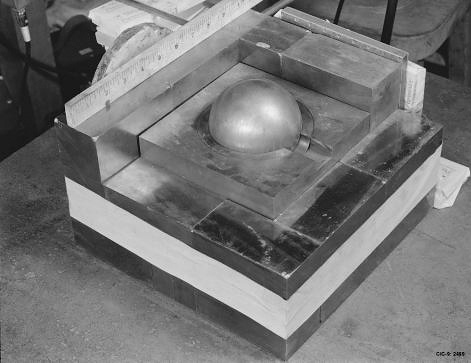
\includegraphics[keepaspectratio, width = 5.0 in]{images/pu_sphere}
    \caption{Plutonium sphere reflected by tungsten-carbide bricks.}
    \label{fig:pu_sphere}
\end{figure}

A second type of accident involves processing operations in which
fissile materials are in solution.  The first domestic processing
accident occured at the Y-12 plant in Oak Ridge, TN.  Y-12 
produces parts from HEU for use in nuclear weapons.  

The accident occured in a portion of the plant used to 
recover HEU from waste material and place it in tanks of favorable
geometry.  These tanks were to be emptied, cleaned, and leak-tested 
with water.  Before the leak-testing began, however, uranium 
solution had leaked from the process stream into the piping
below the storage tanks (and actually into one of the tanks,
as its release valve had been let open).  When the other tanks, full
of water, were emptied, the uranium solution and water accumulated
in a 55 gallon drum.  A nearby worker first noticed dark yellow
fumes followed by a blue flash.  Eight workers received significant
doses, though none died as a result of acute effects.

A rather complete history of criticality accidents in the U.S. and
around the world is contained in the latest edition of
 \textit{A Review of Criticality Accidents} from Los Alamos.  This
document is a really great piece of nuclear history, and students
are highly encouraged to skim through the many accidents covered.

%------------------------------------------------------------------------------
% Computational Aspects
%------------------------------------------------------------------------------

\section*{Computational Aspects}

The intent of this section to provide the reader with an 
overview of criticality safety analysis validation. A brief 
review of regulations and guidance pertinent to criticality safety of 
fissile materials outside reactors is given, with a particular emphasis on 
requirements for ensuring subcritical conditions. The traditional approach to 
bias determination is discussed, and one specific method used in practice
is described and demonstrated in an illustrative example. Subsequently, 
modern S/U-based validation techniques are discussed, and an 
illustrative example is provided and related to the traditional approach.

%------------------------------------------------------------------------------

\subsubsection{Subcritical Limits}

As noted above, ANSI/ANS-8.1 provides guidance 
for avoiding criticality accidents during handling of fissionable material 
outside of reactors \cite{ans8}. The standard provides basic safety principles 
in addition to several limits for simple systems of single isotopes.  
Specifically, the standard defines a \textit{subcritical limit} to be ``the 
limiting value assigned to a controlled parameter that results in a subcritical 
system under specified conditions. The parameter limit allows for 
uncertainties in the calculations and experiemental data used in the derivation 
but not for contingencies.''

These limits are \textit{absolute maxima}, and since they do not include 
contingencies, in practice, adminstrative margins are employed.  A typical 
value, as we'll see below, tends to be 5\% on \keff.

Table \ref{tbl:controlparams} gives several examples of single control 
parameters used in criticality safety analysis.  Note, while ANSI/ANS 8.1 
specifies limits in terms of a single parameter, in some cases, multiple 
parameter limits are also employed.  The standard suggests a few examples, and
cites the technical literature for further guidance. However, while less 
conservative, multiple 
parameter limits require additional adminstrative margins and may be harder to 
use in validation.

\begin{table}[ht]
    \caption{Example single parameters and subcritical limits.}
    \begin{center} 
    \begin{tabular*}{0.90\textwidth}{@{\extracolsep{\fill}} ll } 
      \toprule 
	parameter &  example limit \\
      \midrule
       fissile mass                    &  0.78 kg ${}^{235}$U in UO$_2$NO$_3$ \\
       dimension (width, volume, etc.) &  6.2   L ${}^{235}$U in UO$_2$NO$_3$ \\
       concentration                   &  11.6 g/L${}^{235}$U in UO$_2$NO$_3$ \\
       enrichment                      &  5\%     ${}^{235}$U in UO$_2$       \\
       fissile mass                    &  20.1 kg ${}^{235}$U in UO$_2$ 
                                          (w/ $\rho \leq 18.81$ g/cc) \\
      \bottomrule 
    \end{tabular*} 
    \end{center} 
    \label{tbl:controlparams}
\end{table}

%------------------------------------------------------------------------------


\subsection*{Criticality Safety Analysis Validation}

While the single parameter limits provide useful guidance, two questions 
naturally arise.  First, how does one actually establish these limits?  And 
second, how does one ensure subcriticality in systems that are much more 
complex than, for example, a sphere?  The answer in both cases is by using 
computational methods validated against experiment.

In addition to the single parameter limits, ANSI/ANS-8.1 provides 
requirements for ensuring computational methods used in criticality safety 
analyses are both valid and within the ``area of applicability'' for specific 
applications. The standard defines the area of applicability as ``limiting 
ranges of material compositions, geometric arrangements, neutron energy 
spectra, and other relevant parameters \ldots within which the bias of the 
calculational method is established'' \cite{ans8}.  In other words, an 
\textit{application} is the system of interest, such as a spent fuel canister 
for shipment and disposal. A computational method is \textit{applicable} if 
it is verified against a set of \textit{experiments} that are similar to the 
application with respect to composition, geometry, and so forth.

A \textit{computational bias} is the systematic 
discrepancy between and experimental data and calculated results. Biases 
have associated uncertainties, which quantify the accuracy and 
precision of calculated values and the uncertainty in measured data.

When computational tools are used in criticality safety analyses, the standard
requires that the bias be established.  Qualitatively, the bias must be 
determined via correlating data from critical experiments to computational 
models of the same experiments using the tool to be validated. 
Typically, the measured and 
computed values of \keff are related, but other physical quantities may 
also be used.  The bias is used to normalize a particular code within its 
area of applicability so that its results, after applying the bias, may be 
used to predict criticality within the bias uncertainty.

Another American National Standard, ANSI/ANS-8-17, further explicates 
use of computational tools by defining specific criteria for establishing 
subcriticality \cite{ans8_17}.  Whenever computational methods are 
used in criticality safety analyses, the standard requires that the calculated 
application multiplication factor $k_a$ must be less than or equal to the 
allowable multiplication factor.

The easiest way to think of this is to note that the largest, ``worst case'' 
value for $k_a$ must be below the smallest, least conservative computed 
estimate.  That is to say, the maximum expected application multiplication 
factor (\ie $k_a + \Delta k_a$) must be less than the minimum expected 
computed value (\ie $k_c - \Delta k_c$) for an applicable critical experiment, 
\ie a real, measured system whose \keff is unity, or an average computed 
\keff for several such experiments.  Mathematically, this can be written as
\begin{equation}
 k_a + \Delta k_a \leq k_c - \Delta k_c \, ,
\end{equation}
or
\begin{equation}
 k_a \leq k_c  - \Delta k_a - \Delta k_c \, .
\end{equation}
For added conservatism, the standard further requires that
\begin{equation}
 k_a \leq k_c - \Delta k_a - \Delta k_c - \Delta k_m \, ,
\label{eq:kapp}
\end{equation}
where the standard defines:

\begin{tabular}{rp{10cm}}
 $k_a$           & is the calculated \keff of the 
                   application system for all normal or credible 
                   abnormal conditions; \\
\end{tabular}

\begin{tabular}{rp{10cm}}
 $k_c$           & is the average \keff from the calculation of 
                   the benchmark criticality experiments. 
                   The experiments used 
                   should be neutronically similar to the application
                   system. If the application system has 
                   parameters beyond the area of applicability established 
                   by the benchmark experiments, then the area of 
                   applicability
                   may be extended using trends in the calculated values 
                   of $k_c$ as functions of those parameters; \vspace{12pt} \\
\end{tabular}

\begin{tabular}{rp{10cm}}
 $\Delta k_a$    & is an allowance for 
                 \begin{itemize}
                   \item statistical or convergence uncertainties in 
                         the computed $k_a$;
                   \item material and fabrication tolerances;
                   \item uncertainties due to geometry or material
                         simplifications and approximations;
                 \end{itemize}  \\
\end{tabular}

\begin{tabular}{rp{10cm}}
 $\Delta k_c$    & is a margin for uncertainty in $k_c$ that includes 
                   allowances for
                 \begin{itemize}
                   \item uncertainties in the critical experiments;
                   \item statistical or convergence uncertainties
                         in the computated $k_c$;
                   \item uncertainties due to extrapolation of $k_c$ 
                         outside the experimental data range;
                   \item uncertainties due to geometry or material
                         simplifications and approximations;
                 \end{itemize}
\end{tabular}

\begin{tabular}{rp{12cm}}
 $\Delta k_m$    & is an arbitrary ``administrative'' 
                   margin to ensure the subcriticality 
                   of $k_a$. \\
\end{tabular}

Eq. \ref{eq:kapp} can be rewritten as
\begin{equation}
 k_a + \Delta k_a + \Delta k_m - \beta + \Delta \beta \leq 1 \, ,
\label{eq:kallow}
\end{equation}
where $\beta = k_c - 1$ is the bias and $\Delta \beta = \Delta k_c$ is the 
uncertainty in the bias.  The definition of $\beta$ is based on the fact 
that critical experiments, by their definition, have \keff = 1, and hence 
the bias is just the difference between the computed value and unity.  By 
convention, the bias is defined such that a \textit{ negative} $\beta$ 
indicates an \textit{ underestimated} \keff\!, which is undesirable.

To ensure subcriticality in the application system, an \textit{ upper 
subcritical limit} is defined as
\begin{equation}
 USL = 1 - \Delta k_m + \beta - \Delta \beta \, ,
\label{eq:usl}
\end{equation}
and from Eq. \ref{eq:kallow}, it is apparent that $k_a + \Delta k_a \leq USL$ 
\cite{lichtenwalter1997cbg}.   Thus, the USL is the maximum value an 
application \keff (plus any uncertainties) may have for which the 
application can, with a high degree of confidence, be considered 
subcritical.  The value $1 - USL$  is the mathematical definition of the 
subcritical margin.  In the event the bias $\beta$ is positive, \ie the 
computed value $k_c$ overestimates \keff\!, current practice is to set 
the bias to zero rather than reduce the subcritical margin.

%------------------------------------------------------------------------------

\subsubsection{Traditional Bias Determination}

In the United States, biases and associated uncertainties and USL's have 
often been found through use of \textit{ trending analysis}.  A suite of 
critical experiments is selected for use in a specific safety analysis 
based on the similarity of the experiments to the safety analysis system.  
Traditionally, this similarity is based on physical parameters that include 
the fissile material, hydrogen-to-fissile atom ratio (H/X), average neutron 
energy group causing fission, and energy of average lethargy causing 
fission (EALF), among others \cite{broadhead2004sau}.

While various methods using trending analysis exist for determining the 
biases and USL's, one common approach, denoted USL$_1$ in the 
literature \cite{broadhead2004sau}, is discussed here to provide at least 
some background of current practice. The following description is largely 
adapted from the technical report in which it was first developed 
\cite{lichtenwalter1997cbg}. 

The method computes $k_c(x)$ as a function of a trending parameter $x$ 
using linear regression.  The bias, $\beta(x)$, is just $k_c(x) - 1$.  .  

A lower confidence band $w(x)$ is statistically computed using current 
experiments and uncertainties as well as a specified confidence.  This 
confidence band defines the value below which an additional computed 
\keff value (\ie not included in the analysis) must be for the additional 
system to be considered subcritical with a high degree of confidence.  
Equivalently, for a given value of the trending parameter $x$, $w(x)$ 
represents the value \textit{ above} which the additional computed value $k_c$ 
will be \textit{ if} the system in question is critical---and this consequently 
implies any negative $\beta(x)$ is no worse than $w(x) - 1$.  Hence, if our 
aim is to ensure the actual \keff of a system is subcritical, then its 
computed value should be \textit{ less} than the appropriate confidence band 
value.

To simplify analyses, the limiting width, $W$, of the confidence band is 
used, which (like $w(x)$) takes into account all uncertainties associated 
with the experiments (\eg experimental, stochastic, etc), and consequently, 
is a statistical measure of $\Delta \beta$.  The width $W$ of the 
confidence band is defined
\begin{equation}
 W = \mathrm{max} \Big \{ w(x) | x_{\mathrm{min}},x_{\mathrm{max}} \Big \} \, ,
\label{eq:confwidth}
\end{equation}
where
\begin{equation}
 w(x) = t_{1-\gamma} s_p \Bigg ( 1 + \frac{1}{n} + 
        \frac{(x-\bar{x})^2}{\sum^n_{i=1} (x_i - \bar{x})^2} \Bigg )^{1/2} \, ,
\end{equation}
and $n$ is the number of critical experiments included in the analysis, 
$t_{1-\gamma}$ is the student-t distribution statistic for $1-\gamma$ 
and $n-2$ degrees of freedom ($\gamma$ is the desired confidence level), 
$\bar{x}$ is the mean value of $x$ in the set of experiments, and $s_p$ 
is the pooled standard deviation for the set of calculations.

The pooled standard deviation $s_p$ is defined by
\begin{equation}
 s^2_p = s^2_{k(x)} + s^2_w \, ,
\end{equation}
where $s^2_{k(x)}$ is the mean-square error of the linear regression, 
defined as
\begin{equation}
 s^2_{k(x)} = \frac{1}{n-2} \Bigg ( \sum^n_{i=1} (k_i - \bar{k})^2 - 
              \frac{\Big(\sum^n_{i=1} (x_i-\bar{x})(k_i -\bar{k}) \Big )^2 }
                   {\sum^n_{i=1} (x_i - \bar{x})^2} \Bigg ) \, ,
\end{equation}
and $s^2_w$ is the variance of the data, defined as
\begin{equation}
 s^2_w = \frac{1}{n} \sum^n_{i=1} \sigma^2_i \, ,
\end{equation}
where  $\sigma_i$ is the uncertainty in the $i$th calculated value, 
accounting for method uncertainty (\eg Monte Carlo statistics) and 
estimated uncertainty due to cross-section uncertainty 
(see Section \ref{sec:uncanal}).

The width of the confidence $W$ is chosen to be the \textit{ maximum} value 
of $w$ at the limits of the range of $x$ corresponding to the experiments 
to be conservative, and moreover, it serves to simplify the definition of 
USL.  Current guidance is to define $W$ at the 95\% confidence level, 
\ie choose $\gamma = 0.95$.  See Section \ref{sec:exampletrends} below 
for an illustrative example of the USL$_1$ methodology.

%------------------------------------------------------------------------------

\subsubsection{S/U-Techniques}

Unfortunately, the proper selection of parameters over which to trend, 
and the experiments with which to trend, is largely based on expert 
judgement.  As experiments continue to become more expensive, use of 
computational methods will grow.  Furthermore, new applications will 
continue to extend beyond the areas of applicability of current 
experimental data, and consequently, methods to extend beyond these 
areas are needed.

For the past several years, ORNL has worked with the support of the 
NRC and the Department of Energy's (DOE) Nuclear Criticality Safety 
Program to develop ``a rigorous physics-based approach for the 
determination of system similarity'' for determining areas of 
applicability \cite{broadhead2004sau}.  Additionally, their efforts 
aimed to develop the methodology and computational tools needed for 
``determination of biases and uncertainties due to experimental 
descriptions, computational methods, and nuclear data.''

As an alternative to traditional trending analysis, work was done to 
develop S/U-based, easily-quantifiable parameters to measure the 
similarity of systems.  It is beyond our scope to describe the 
methods in detail.  Interested readers should see the exercises
of Lecture \ref{lec:the_adjoint_and_perturbation_theory} for some
basic theory needed to derive the results, and Ref. 
\cite{broadhead2004sau} for greater detail.

Skipping the theory, what we end up with is the sensitivity
of \keff to the various underlying nuclear data, 
\begin{equation}
 S_{k,\sigma_x} = \frac{\sigma_x}{k}\frac{\partial k}{\partial \sigma_x} 
 \label{eq:keffsens}
\end{equation}
where $x$ denotes some reaction of interest.  We express the sensitivity 
of \keff to all nuclides in a system as the vector $\mathbf{S}_k$,
which can implicitly represent dependence on multigroup data.

Sensitivity vectors can be used to compare both the qualitative and 
quantitative similarity between two systems with respect to single or 
several nuclide-reactions. Let the entire set of group-wise, nuclide-reaction 
cross-sections be denoted 
$\bm{\sigma} \equiv \sigma_i, \; \; n = 1,\;2,\ldots,N$, where $N$ is the 
total number of nuclide-reactions multiplied by the number of energy 
groups.  The $N\times N$ correlation (\ie relative covariance) matrix 
of $\bm{\sigma}$ is defined
\begin{equation}
\mathbf{C_{\sigma \sigma}} \equiv \Bigg[\frac{\mathrm{COV}(\sigma_i,\sigma_j)}
                                             {\sigma_i \sigma_j} \Bigg ] \, ,
\end{equation}
where $i$ and $j$ range from 1 to $N$, and 
\begin{equation}
\mathrm{COV} = \langle (\sigma_i - \bar{\sigma_i})(\sigma_j - 
               \bar{\sigma_j}) \rangle 
             = \langle \delta \sigma_i \delta \sigma_j \rangle \, ,
\end{equation}
where $\bar{\sigma_i}$ represents the expected value of the data $\sigma_i$.  

Because the components of \cov represent relative uncertainties, and because 
from above, we know the \keff sensitivity represents the relative change in 
\keff due to relative changes in some nuclide-reaction data, the relative 
uncertainty in \keff is therefore
\begin{equation}
\frac{\delta k}{k} = \sqrt{ \mathbf{S}_k \mathbf{C_{\sigma \sigma}} 
                     \mathbf{S}_k^T } \, ,
\end{equation}
where $T$ denotes the matrix transpose.  If several systems are of interest, 
then an $N \times I$  matrix of sensitivity vectors $\mathbf{\bar{S}}_k$ can 
be defined, where $I$ is the number of systems.  By folding 
$\mathbf{\bar{S}}_k$ with \cov, one obtains
\begin{equation}
 \mathbf{C}_{kk} =  \mathbf{\bar{S}}_k \mathbf{C_{\sigma \sigma}} 
                    \mathbf{\bar{S}}_k^T  \, ,
\label{eq:kunc}
\end{equation}
an $I\times I$ matrix consisting of each system's relative variance in 
\keff (\ie $(\Delta k/k)^2$) due to data uncertainties (the diagonal terms, 
$\alpha_{ii}$) and the relative covariances in \keff between systems 
(the off-diagonal terms, $\alpha_{ij}$).  These off-diagonal terms 
represent ``shared variance'' or ``shared uncertainty'' between systems.  

The correlation coefficient between system $i$ and $j$ is defined
\begin{equation}
 c_{k} =  \frac{\alpha^2_{ij}}{\alpha_i \alpha_j}  \, ,
\label{eq:ck}
\end{equation}
which, as is expected, takes on values between -1 
(completely anti-correlated) and 1 (completely correlated). 
A value $c_k = 0$ indicates no correlation between systems.  

The correlation of two systems is greatest if they share basic 
characteristics, \eg fuel type, moderator, other materials.  Two 
water-moderated thermal UO$_2$ systems would be expected to have 
a higher degree of correlation than would such a thermal system 
and a molten salt fast reactor.  Use of $c_k$ as a trending 
parameter in the USL$_1$ method is illustrated below.

%------------------------------------------------------------------------------

\subsubsection{Example Analyses}

To illustrate the USL$_1$ method using both traditional parameters 
and $c_k$, 25 thermal LEU systems were chosen for example analyses.  
Two additional systems were selected as ``applications'' for which 
the $\beta$, $\Delta \beta$, and the USL are determined\footnote{The 
minimum recommended number of experiments for trending with the 
USL$_1$ method is 25; here, just the minimum was used for these example 
cases.}. The experiments range from 2.35\% to 5\% enrichement, and have 
EALF values ranging from 0.017 to 2.24 eV.  %These parameters, along 
%with $c_k$ with respect to the two applications (LCT-079-002 and 
%LCT-050-001), are provided in Table \ref{tbl:exampletrend}. 
All experiments 
are included in the International Handbook of Evaluated Criticality Benchmark 
Experiments \cite{ihecsbe} and are low enriched uranium, thermal assemblies.
The LCT-079 and LCT-050 are experiments
of use to burnup credit, a topic discussed below; however, their use here
is purely for example.  

Figures \ref{fig:trend_ealf}-\ref{fig:trend_ck2} show the trending analysis 
for using EALF, enrichment, and $c_k$.  For both EALF and enrichment, only 
one analysis was needed for the applications since neither parameter depends 
on the application.  However, separate cases were run using $c_k$ values 
specific to the given application.  The experiments are the black dots, 
and the applications are red shapes.  For all cases, the uncertainty is 
computed using Eq. \ref{eq:kunc}, where the uncertainty for the system is 
its associated diagonal element of $\mathbf{C}_{kk}$, \ie the uncertainty 
in cross-sections propagated to \keff via use of sensitivity profiles.  
This is in line with previous analyses \cite{broadhead2004sau}.  Note, for 
the USL, an administrative margin of $\Delta k_m = 0.05$ was used.

% \begin{table}[hp]
%  \caption{Experiment and test application parameters.  Note (a) and (b) refer to the LCT-079 and LCT-050 experiments.}
%  \begin{center} 
%  \begin{tabular*}{0.95\textwidth}{@{\extracolsep{\fill}} ccccccc } 
%   \toprule 
%          Id.       &  \keff   & $\sigma_k$&  EALF (eV)&  Enrich.(\%) & $c_k$ (a) & $c_k$ (b)    \\ 
%    \midrule
%   LCT-010-005  &  0.9951  &  0.0050  &  3.89E-01  &  4.306  &  0.861  &  0.890  \\
%   LCT-010-016  &  0.9936  &  0.0058  &  2.92E-01  &  4.306  &  0.977  &  0.982  \\
%   LCT-010-017  &  0.9937  &  0.0058  &  2.86E-01  &  4.306  &  0.979  &  0.983  \\
%   LCT-010-018  &  0.9924  &  0.0058  &  2.81E-01  &  4.306  &  0.980  &  0.985  \\
%   LCT-010-019  &  0.9917  &  0.0058  &  2.74E-01  &  4.306  &  0.980  &  0.986  \\
%   LCT-017-003  &  0.9927  &  0.0055  &  9.57E-02  &  2.350  &  0.899  &  0.924  \\
%   LCT-017-004  &  0.9919  &  0.0052  &  2.17E-01  &  2.350  &  0.827  &  0.850  \\
%   LCT-017-005  &  0.9945  &  0.0053  &  1.89E-01  &  2.350  &  0.851  &  0.876  \\
%   LCT-017-006  &  0.9939  &  0.0054  &  1.78E-01  &  2.350  &  0.862  &  0.888  \\
%   LCT-017-007  &  0.9937  &  0.0053  &  1.69E-01  &  2.350  &  0.858  &  0.884  \\
%   LCT-042-001  &  0.9906  &  0.0054  &  1.73E-01  &  2.350  &  0.797  &  0.764  \\
%   LCT-042-002  &  0.9909  &  0.0055  &  1.79E-01  &  2.350  &  0.801  &  0.767  \\
%   LCT-042-003  &  0.9897  &  0.0054  &  1.86E-01  &  2.350  &  0.779  &  0.747  \\
%   LCT-042-004  &  0.9918  &  0.0054  &  1.84E-01  &  2.350  &  0.768  &  0.736  \\
%   LCT-042-005  &  0.9921  &  0.0057  &  1.81E-01  &  2.350  &  0.891  &  0.862  \\
%   LCT-049-001  &  0.9904  &  0.0057  &  2.02E+00  &  5.000  &  0.889  &  0.860  \\
%   LCT-049-002  &  0.9914  &  0.0057  &  2.03E+00  &  5.000  &  0.895  &  0.867  \\
%   LCT-049-003  &  0.9913  &  0.0055  &  2.15E+00  &  5.000  &  0.877  &  0.849  \\
%   LCT-049-004  &  0.9906  &  0.0058  &  2.24E+00  &  5.000  &  0.932  &  0.910  \\
%   LCT-049-005  &  0.9915  &  0.0059  &  1.14E+00  &  5.000  &  0.934  &  0.911  \\
%   LCT-049-006  &  0.9900  &  0.0055  &  1.15E+00  &  5.000  &  0.889  &  0.894  \\
%   LCT-049-007  &  0.9904  &  0.0053  &  1.11E+00  &  5.000  &  0.873  &  0.878  \\
%   LCT-049-008  &  0.9906  &  0.0053  &  1.19E+00  &  5.000  &  0.862  &  0.867  \\
%   LCT-049-009  &  0.9912  &  0.0053  &  7.39E-01  &  5.000  &  0.869  &  0.873  \\
%   LCT-049-010  &  0.9904  &  0.0053  &  7.47E-01  &  5.000  &  0.869  &  0.874  \\
%   \midrule
%   LCT-079-002  &  0.9897  &  0.0069  &  2.03E+00  &  4.310  &  1.000  &  na     \\
%   LCT-050-001  &  0.9906  &  0.0067  &  1.99E-01  &  4.738  &  na     &  1.000  \\
%   \bottomrule 
%  \end{tabular*} 
%  \end{center} 
%  \label{tbl:exampletrend}  
% \end{table}

\begin{figure}[htp] 
    \centering
    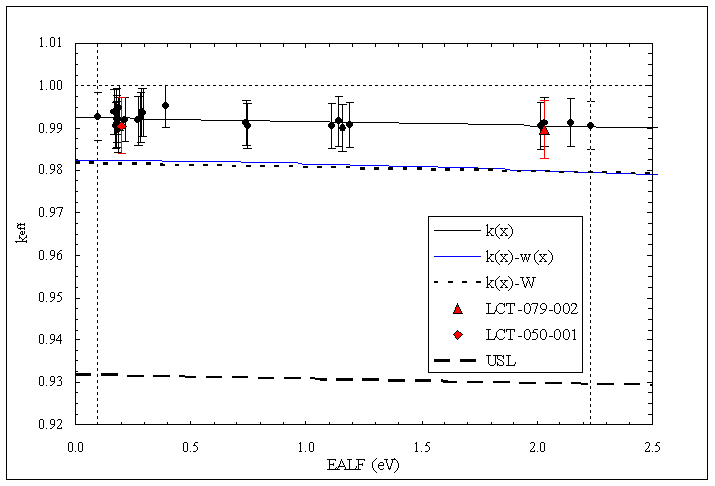
\includegraphics[keepaspectratio, width = 5 in]{images/trend_ealf}
    \caption{Example trending analysis using EALF.}
    \label{fig:trend_ealf}
\end{figure}


\begin{figure}[htp] 
    \centering
    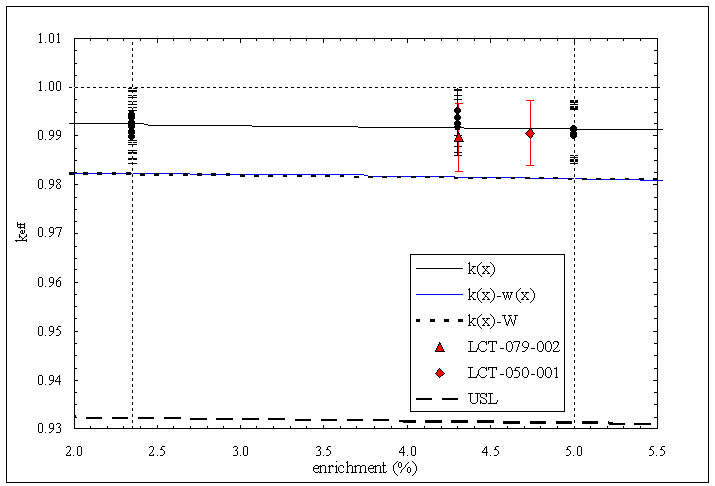
\includegraphics[keepaspectratio, width = 5 in]{images/trend_enrich}
    \caption{Example trending analysis using enrichment.}
    \label{fig:trend_enrich}
\end{figure}


\begin{figure}[htp] 
    \centering
    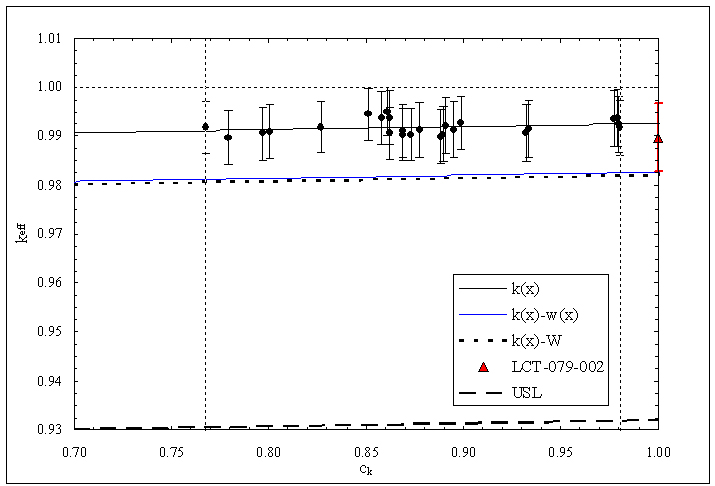
\includegraphics[keepaspectratio, width = 5 in]{images/trend_ck1}
    \caption{Example trending analysis using $c_k$ (for LCT-079-002).}
    \label{fig:trend_ck1}
\end{figure}


\begin{figure}[htp] 
    \centering
    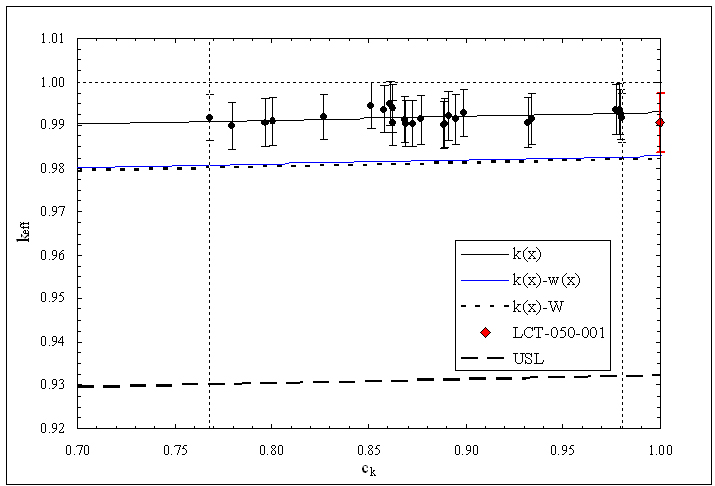
\includegraphics[keepaspectratio, width = 5 in]{images/trend_ck2}
    \caption{Example trending analysis using $c_k$ (for LCT-050-001).}
    \label{fig:trend_ck2}
\end{figure}

From the trends, the bias $k(x)-1$ (where $x$ is the parameter value 
for the application) and associated bias uncertainty (\ie $W$ from 
Eq. \ref{eq:confwidth}) can be computed in addition to the USL.  
Since the ``applications'' are known critical experiments, it is useful 
to compare the observed bias (\ie $k_{\mathrm{calc}} -1$) to the bias 
as predicted via trending.  Table \ref{tbl:trendbias} provides the 
observed and predicted biases (with uncertainty) and the USL for both 
applications.  For each application, all three methods yield very similar 
USL's, and all the biases are slightly underpredicted but well within 
one standard deviation of the observed biases.  

With such a large $\Delta k_m$, it is easy to wonder why we care 
about $\Delta \beta$. However, if we interpret subtracting $\Delta k_m$ 
from \keff as simply shifting the definition of critical, then it 
becomes clearer that $\Delta \beta$ is still important.

{\tiny
\begin{table}[hp]
 \caption{Observed and predicted biases ($\beta_{\mathrm{ob}}$ and 
         $\beta$), $\Delta \beta$, all in percent, and USL using 
         each trending technique.}
 \begin{center} 
 \begin{tabular*}{0.98\textwidth}{@{\extracolsep{\fill}} c|cccc|cccc } 
  \toprule
              & \multicolumn{4}{c}{LCT-079-002}          & \multicolumn{4}{c}{LCT-050-001} \\
   \midrule 
             & $\beta_{\mathrm{ob}}$ & $\beta$ & $\Delta \beta$  & USL & $\beta_{\mathrm{ob}}$& $\beta$  & $\Delta \beta$ & USL \\ 
   \midrule
       EALF  &  -1.08  &  -0.95  &  1.08  &  0.9298  &  -0.94  &  -0.77  &  1.08  &  0.9316 \\
    Enrich.  &  -1.08  &  -0.84  &  1.02  &  0.9314  &  -0.94  &  -0.85  &  1.02  &  0.9313 \\
      $c_k$  &  -1.08  &  -0.74  &  1.16  &  0.9306  &  -0.94  &  -0.71  &  1.07  &  0.9322 \\
  \bottomrule 
 \end{tabular*} 
 \end{center} 
 \label{tbl:trendbias}  
\end{table} 
}

\section*{Case Study: Burnup Credit}

\subsubsection*{Overview and Motivation}

The transportation and storage of used nuclear fuel is an integral component of any
nuclear fuel cycle. During handling of used nuclear fuel, strict attention must be paid
to criticality safety. The chief concern of criticality safety is to ensure the effective
multiplication factor \keff of the system in question is below unity at all times, i.e. to
ensure subcriticality.
For the case of used nuclear fuel, several factors affect the subcritical margin, i.e.
by how much a system is subcritical. Typical, unirradiated light water reactor (LWR)
fuel consists of uranium-oxide (UO2 ) enriched to 3-5\% ${}^{235}$U. During its time in the
reactor, nuclear fuel undergoes significant compositional changes, a process referred
to as burnup. Most importantly, the fissile isotope 235 U is depleted, generating various
fission products (FP's), many of which are parasitic neutron absorbers. Simultaneously,
${}^{235}$U breeds ${}^{239}$Pu which also undergoes fission and produces FP's. The net
effect of these compositional changes is to decrease the \keff of the fuel with increased
burnup. Accounting for this decrease in \keff (or equivalently, a decrease in reactivity)
in subcritical margins is often referred to as \textit{burnup credit}.

Historically, the so-called \textit{fresh fuel assumption} was used as a conservative bound
in criticality safety analysis of used nuclear fuel [1]. More recently, the Nuclear
Regulatory Commission (NRC) offered guidance for crediting the major (fissile) actinides
in such analyses in its Interim Staff Guidance - 8, revision 2 (ISG-8R2) report [2]. However,
even this results in a very conservative estimate of the subcritical margin of used
nuclear fuel.

Changes in the major actinides account for about 66-75\% of the net reduction
in reactivity; FP's account for the remainder, the percentages depending on burnup.
The FP's relevant to burnup credit, roughly in order of importance, include SM.
 
Why do we care?  Naturally, assuming a canister of some number of burned assemblies 
contains only fresh fuel is quite conservative.  Figure \ref{fig:loading_curve} shows 
loading curves for a generic used fuel canister with 32 WH 17x17 assemblies of varying 
initial enrichments and burnups.  Configurations below a given line do not meet subcritical 
limits under the given assumptions.  The reference case assumes fresh fuel, and each 
subsequence curve relaxes the assumptions.  

Considering that much of the current U.S. inventory of used fuel lies below the reference 
curve, a 32-assembly canister could not be widely used (and instead, canisters such as
the 21-assembly Transportation, Aging, and Disposal (TAD) canister intended for ultimate
disposition in Yucca Mountain would be required).  The cost of producing, loading, shipping, 
and disposing canisters is not negligible, and a study by Parks and Wagner suggest that
crediting the FP's in criticality safety analysis, thus allowing the high capacity
canisters, would potentially save upwards of \$200 million dollars in total disposal
costs \cite{parks2004csp}. 

\begin{figure}[ht] 
    \centering
    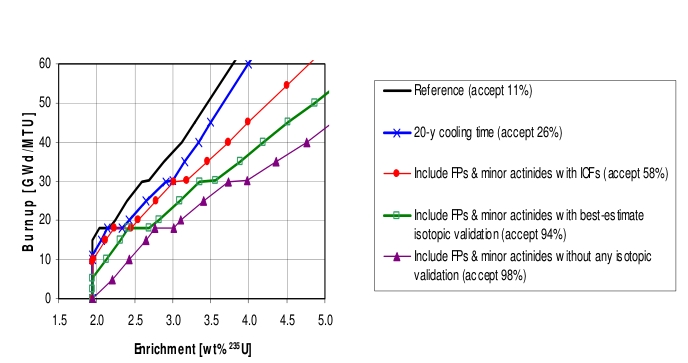
\includegraphics[keepaspectratio, width = 5.0 in]{images/loading_curve}
    \caption{Effect of calculational assumptions on loading curves for the GBC-32 and WH 17x17 assemblies.}
    \label{fig:loading_curve}
\end{figure}

\subsubsection*{Current Research}

To take into account the reduction in reactivity due to fission products,
called \textit{full burnup credit}, requires adequate knowledge of the 
isotopic content of the spent fuel (via validated depletion methods), and, 
our focus here, \textit{methods} to determine criticality and 
\textit{experiments} to validate those methods.

Current work has expanded on the S/U-based techniques
outlined above to develop methods for determinining biases of 
individual nuclides. While the details are beyond our scope, we give 
a brief description and several references for interested readers.

The basis of the work is the generalized linear least-square method (GLLSM).
GLLSM takes as input a set of nuclear data and covariances, the sensitivities 
of experiment models to nuclear data, the model \keff and uncertainty,
the experiment \keff and uncertainty (and any experiment correlation), 
and \textit{adjusts the nuclear data}
so that the the experiment and model \keff match.  It does so in a way that
minimizes the variation of all parameters (data and \keff) in terms of the
standard deviations of those parameters.  In other words, for all parameters
$p$, the method forces the experiment and model \keff to match while 
minimizing $\sum_i (\Delta p_i / \sigma_{p_i})^2$.  The adjustments can be 
propogated to an application's \keff via its model sensitivities, and the 
resulting difference is the bias.

To find biases of individual nuclides, the GLLSM method can be applied to 
so-called ``replacement experiments''.  These experiments consists of a single
reference case, and one or more cases that introduce some small perturbation
to the system, such as small foils of a fission product between fuel pellets 
\cite{buccx} or small concentrations of a fission product in a bulk
moderator \cite{french}.  GLLSM can then be applied to the reactivity 
difference between a reference-perturbation pair of models and experiements 
(rather than on the eigenvalue), since the sensitivities of the 
reactivity difference should be small for all but the perturbation 
material.  Consequently, the corresponding adjustment to the data should 
primarily be due to the test material, and as above, the adjustment can 
be propogated to the application to define a nuclide-specific bias.

\subsubsection{Limitations}

Two significant limitations apply to the methods under development.  First,
the methods require that relevant experiments are available.  However,
only a handful of experiments have been performed relevant to burnup credit,
and of those, the difference between reference and perturbation cases may 
be too high to extract partial biases.  Moreover, little data is available
for the correlation between experiments.  For the the reactivity difference
method described above, the resulting biases are extremely sensitive to 
the correlation between experiments. This suggests that future 
experiments should be designed with the various S/U methods as guidance.

A second, perhaps more significant issue is the general lack of reliable
nuclear covariance data.  Only for the most important isotopes does credible
data exist (such as uranium isotopes).  For isotopes of generally less
importance (like many fission products), little if any covariance data
exists.  Until reliable covariance data exists, the methods described
above are of limited value.
 
\section{Further Reading}

Much of the content in this lecture was inspired by Knief's 
\textit{Nuclear Criticality Safety: Theory and Practice} \cite{knief}.  Of
course, in one lecture, all that material cannot be covered, and the student
is directed to that book for more info most of the topics addressed here.
A more succinct overview of some of the topics is given by 
Peavey
in the \textit{Handbook of Nuclear Engineering} \cite{handbook}.  

For an overview of the application of sensitivity and uncertainty analysis
to criticality safety, see Broadhead et. al \cite{broadhead2004sau}, and
for the latest work on adjustment techniques applicable to full burnup
credit, see Rearden et al. \cite{reardenNT}.
% 
\part{Deterministic Transport} 

\chapter{The Transport Equation}

In this lecture, we introduce general \textit{transport equations} and finish by developing the form used in neutron transport theory.  In the lectures to follow, we shall describe other aspects of the neutron transport equation and methods by which it can be solved both analytically and numerically.

\section*{Transport Theory}

Transport theory aims to describe mathematically the movement (i.e. ``transport'') of particles as they traverse a medium.  For example, we might describe the transport of high energy gammas through a lead shield, or the movement of neutrons through uranium dioxide pellets.  We might also describe the movement of particles in a dense gas as they navigate through a medium consisting of the gas itself.

In all cases, transport theory describes such processes in an \textit{average} sense.  For instance, we do not compute the individual trajectories of neutrons in a reactor via transport theory.  That, instead, would require molecular dynamics, in which Newton's equation of force is solved for the many-bodied problem of all neutrons in the vicinity of interest (an essentially impossible problem), or perhaps the Monte Carlo methods described in previous lectures, where a sample of individual particles are tracked to approximate ensemble averages (a difficult, but as we've seen, tractable problem).  Hence, the quantities we shall compute using the equations of transport theory should be recognized as expected and not exact values.

\section*{Fundamental Quantities}

We begin by defining several fundamental quantities.  It should be noted that the forms introduced at first are likely different from what you might have seen in a previous reactor physics course.  The purpose here is two-fold.  First, we wish to introduce the quantities and eventually the equations in a general way to make clear that transport theory is not restricted to the neutron transport equation.  Second, for those who might be familiar with e.g. the Boltzmann equation of gas dynamics (and not neutron transport), the notation will be familiar and lead smoothly into our more familiar form.

We first define the \textit{phase space density function}, the knowledge which we can use to compute essentially all quantities of interest:
\begin{center}
  \begin{tabular}{cp{7.0cm}}
    $n(\mathbf{r},\mathbf{v},t)d^3r d^3v \equiv $ &
    expected number of particles in  $d^3r$  about  $\mathbf{r}$  with velocity  $dv$ about  $\mathbf{v}$ at time $t$.  
  \end{tabular}
\end{center}
It is often most convenient to break the velocity into its scalar (speed) and vector (direction) components.  The scalar component is recast in the energy variable via $E = mv^2/2$, and the direction vector is defined $\mathbf{\Omega}=\mathbf{v}/|\mathbf{v}|$.  The phase space density can then be rewritten as
\begin{center}
  \begin{tabular}{cp{7.0cm}}
    $n(\mathbf{r},\mathbf{\Omega},E,t)d^3r d\Omega dE \equiv $ &
    expected number of particles in  $d^3r$  about  $\mathbf{r}$  going in the directions $d\Omega$ about $\mathbf{\Omega}$ with energy  $dE$ about  $E$ at time $t$.  
  \end{tabular}
\end{center}
In this form, $n(\mathbf{r},\mathbf{\Omega},E,t)$ is often referred to as the angular density.

\begin{wrapfigure}{r}{0.5\textwidth}
    \begin{center}
    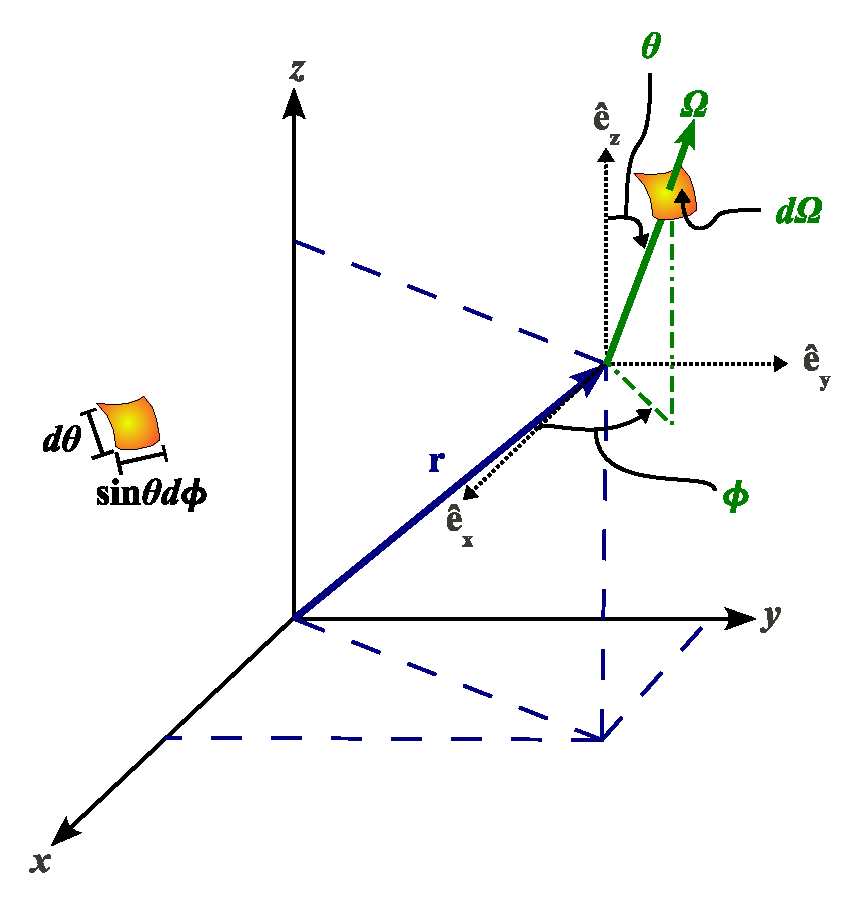
\includegraphics[keepaspectratio, width = 2.7 in]{images/phase_space}
    \end{center}
    \caption{Schematic of Phase Space.}
    \label{fig:phase_space}
\end{wrapfigure}

We can relate the phase space densities in terms of $\mathbf{v}$ and $(E,\mathbf{\Omega})$ via the relations
\begin{equation}
 \begin{split}
  n(\mathbf{r},E,\mathbf{\Omega},t) &= (v/m) n(\mathbf{r},\mathbf{v},t) \\
  n(\mathbf{r},E,\mathbf{\Omega},t) &= (1/mv) n(\mathbf{r},v,\mathbf{\Omega},t) \\
  n(\mathbf{r},v,\mathbf{\Omega},t) &= v^2 n(\mathbf{r},\mathbf{v},t) \, ,
 \end{split}
 \label{eq:densityrelations}
\end{equation}
proofs of which are left as exercises.

Figure \ref{fig:phase_space} depicts a schematic of the phase space used in terms of the position $\mathbf{r}$ and direction $\mathbf{\Omega}$.  The position vector is further broken down into the polar angle $\theta$ and azimuthal angle $\phi$.  The differential solid angle element $d\Omega$ is also shown, and can be expressed in terms of $\theta$ and $\phi$ via
\begin{equation*}
 d\Omega = \sin{\theta} d\theta d\phi \, .
\end{equation*}  
One might envision such solid angle elements as the small bumps on basketballs.  

A quantity closely related to the phase space density (or current density) is the \textit{angular current density}:
\begin{center}
  \begin{tabular}{cp{5.0cm}}
    $\mathbf{j}(\mathbf{r},\mathbf{v},t)\cdot d\mathbf{S} d^3v = \mathbf{v} n(\mathbf{r},\mathbf{v},t) \cdot d\mathbf{S} d^3v \equiv $ &
    expected number of particles that cross an area $dS$ per second with velocity $d^3v$ about $\mathbf{v}$ at time $t$.
  \end{tabular}
\end{center}

We can also define \textit{partial currents} with respect to a particular surface $S$ defined by an outward normal vector $\mathbf{\hat{e}}_s$:

\begin{center}
  \begin{tabular}{cp{5.0cm}}
    $J_{\pm}(\mathbf{r},t) = \pm \int_{\pm} d^3v  \mathbf{\hat{e}}_s \cdot \mathbf{j} (\mathbf{r},\mathbf{v},t) \equiv $ &
   the rate at which particles flow through $S$ in the outward (+) or inward (-) direction.
  \end{tabular}
\end{center}

The \textit{current density} $\mathbf{J}(\mathbf{r},t)$ is defined by integrating the angular current density over all velocities.  Then for our surface $S$, the net rate of particles passing outward through $S$ is just $\mathbf{J}(\mathbf{r},t) \cdot \mathbf{\hat{e}}_s$.  From our definition of partial currents, the net current passing outward must also be $J_+ - J_-$, yielding the useful identity
\begin{equation}
 \mathbf{J}(\mathbf{r},t) \cdot \mathbf{\hat{e}}_s = J_{+}(\mathbf{r},t) - J_{-}(\mathbf{r},t) \, .
 \label{eq:net2partial}
\end{equation}

%A point of caution: it should be noted that $n$ and $\mathbf{j}$ must have the same units but represent wholly different things since $n$ is a scalar quantity while $\mathbf{j}$ is a vector quantity.  This will be true also of $\mathbf{J}$ and the scalar flux $\phi$, which will be introduced

Of particular interest to us in the next section will be reaction rates, which can most easily be described using the \textit{angular flux}
\begin{center}
  \begin{tabular}{cp{2.0cm}}
    $ \psi (\mathbf{r},\mathbf{\Omega},E,t) = v n(\mathbf{r},\mathbf{\Omega},E,t) \equiv $ &
    angular flux
  \end{tabular}
\end{center}
and \textit{scalar flux}
\begin{center}
  \begin{tabular}{cp{2.0cm}}
    $ \phi (\mathbf{r},E,t) = \int_{4\pi} d\Omega \psi (\mathbf{r},\mathbf{\Omega},E,t)  \equiv $ &
    scalar flux.
  \end{tabular}
\end{center}

\section*{A General Transport Equation}

Consider an arbitrary volume $V$ with a surface $S$.  Our goal is to represent the time rate of change of the particle density $n(\mathbf{r},\mathbf{v},t)$ within the volume.  Neglecting external forces, the only factors affecting the density are collisions within the volume that change a particle's velocity, the streaming of particles into and out of the surface, and any internal source of particles.  This simple balance can be expressed mathematically as
\begin{equation}
\begin{split}
 \overbrace{ \frac{\partial}{\partial t} \Bigg ( \int_V d^3 r n(\mathbf{r},\mathbf{v},t) \Bigg ) }^{\text{total rate of change of }n\text{ in } V} 
      &=  - \overbrace{\int_S dS \mathbf{\hat{e}}_S \cdot \mathbf{j}(\mathbf{r},\mathbf{v},t) }^{\text{streaming rate}}
       + \overbrace{ \int_V d^3 r \Big( \frac{\partial n}{\partial t} \Big )_{\mathrm{coll}} }^{\text{collision rate}} \\
      &+ \underbrace{ \int_V d^3 r s(\mathbf{r},\mathbf{v},t) }_{\text{source emission rate}}  \, ,
\end{split}
\label{eq:balance}
\end{equation}
where $s$ represents a source inside the volume and $(\partial n/\partial t)_{\mathrm{coll}}$ is the time rate of change due to collisions, specific forms of which are application-dependent and will be discussed below.  Note the minus sign on the surface integral, i.e. the streaming term.  Since the integral describes the net rate of neutrons going \textit{out} of the surface, we negate it so that a positive net rate directed inward is a positive contribution to the total time rate of change of $n$ in $V$.

Eq. \ref{eq:balance} gives us a simple relation in terms of both volume and surface integrals.  Our life is always easiest if we have the same integration on both sides.  By the divergence (or Gauss') theorem, we can rewrite the streaming term
\begin{equation}
 \int_S dS \mathbf{\hat{e}}_S \cdot \mathbf{j}(\mathbf{r},\mathbf{v},t) = \int_V d^3r \nabla \cdot \mathbf{j}(\mathbf{r},\mathbf{v},t) \, .
\end{equation}
Since $\nabla$ acts on $\mathbf{r}$ and not $\mathbf{v}$, we note $ \nabla \cdot \mathbf{j} = \nabla \cdot (\mathbf{v} n) =  \mathbf{v} \cdot \nabla n + \overbrace{ n \nabla \cdot \mathbf{v}}^{\to 0} = \mathbf{v} \cdot \nabla n$.  Hence, the streaming term becomes
\begin{equation}
 \int_V d^3r \nabla \cdot \mathbf{j}(\mathbf{r},\mathbf{v},t) = \int_V d^3r \mathbf{v} \cdot \nabla n(\mathbf{r},\mathbf{v},t) \, .
\end{equation}

For a constant volume, $(\partial/\partial t) \int_V d^3 r n = \int_V d^3 (\partial n/\partial t)$, and so our balance equation can be rewritten as
\begin{equation}
\begin{split}
 \overbrace{  \Bigg ( \int_V d^3 r \frac{\partial}{\partial t}n(\mathbf{r},\mathbf{v},t) \Bigg ) }^{\text{total rate of change of }n\text{ in } V} 
      &=  - \overbrace{\int_V d^3r \mathbf{v} \cdot \nabla n(\mathbf{r},\mathbf{v},t)}^{\text{streaming rate}}
       + \overbrace{ \int_V d^3 r \Big( \frac{\partial n}{\partial t} \Big )_{\mathrm{coll}} }^{\text{collision rate}} \\
      &+ \underbrace{ \int_V d^3 r s(\mathbf{r},\mathbf{v},t) }_{\text{source emission rate}}  \, .
\end{split}
\label{eq:balance2}
\end{equation}
For an arbitrary volume $V$, the integrands of Eq. \ref{eq:balance2} must vanish, yielding a general transport equation:
\begin{equation}
  \frac{\partial}{\partial t}n(\mathbf{r},\mathbf{v},t) = -\mathbf{v} \cdot \nabla n(\mathbf{r},\mathbf{v},t) + \Big( \frac{\partial n}{\partial t} \Big )_{\mathrm{coll}} +  s(\mathbf{r},\mathbf{v},t) \, .
\end{equation}

\section*{Even More Generality}
We can skip the differential volume formulation by considering the material derivative of $n$ (using Cartesian coordinates):
\begin{equation}
 \begin{split}
 \frac{Dn}{Dt} &\equiv \frac{ \partial n}{\partial t} 
 + \frac{\partial x}{\partial t}\frac{\partial n}{\partial x} + \frac{\partial y}{\partial t}\frac{\partial n}{\partial y} + \frac{\partial z}{\partial t}\frac{\partial n}{\partial z} +  \frac{\partial v_x}{\partial t}\frac{\partial n}{\partial v_x} +  \frac{\partial v_y}{\partial t}\frac{\partial n}{\partial v_y} +  \frac{\partial v_z}{\partial t}\frac{\partial n}{\partial v_z} \\
               &= \frac{ \partial n}{\partial t} + \mathbf{v}\cdot \nabla n + \mathbf{a} \cdot \nabla_{\mathbf{v}} n \\
               &= \frac{ \partial n}{\partial t} + \mathbf{v}\cdot \nabla n + \frac{\mathbf{F}}{m} \cdot \nabla_{\mathbf{v}} n \, ,\\
 \end{split}
\end{equation}
where $\nabla_{\mathbf{v}}$ is the gradient operator with respect to velocity components (rather than spatial coordinates).  The material derivative is the total time rate of change, accounting for convective (streaming) effects as well as the influence of an external force $\mathbf{F}$, a factor we did not account for above.  

This total rate of change must be balanced by sources and sinks, which are the collision and internal source terms.  Hence, an even more general transport equation can be written
\begin{equation}
  \frac{\partial n}{\partial t} + \mathbf{v} \cdot \nabla n + \frac{\mathbf{F}}{m} \cdot \nabla_{\mathbf{v}} n =   \Big( \frac{\partial n}{\partial t} \Big )_{\mathrm{coll}} +  s \, .
 \label{eq:generalte}
\end{equation}

\section*{Neutron Transport}

To arrive at the neutron transport equation, we bring back the macroscopic cross-sections studied in Lecture \ref{lec:macro}.  Using our definition for the scalar flux, the volumetric collision rate at a particular point in phase space and time is simply
\begin{equation}
 R_{\text{coll}}(\mathbf{r},\mathbf{\Omega},E,t) = \psi(\mathbf{r},\mathbf{\Omega},E,t) \Sigma_t(\mathbf{r},E) \, .
\end{equation}
However, we know that neutrons at one energy and angle can scatter into another energy and angle, and so in general, the rate at which neutrons at any angle and energy are scattered into a particular energy and angle is
\begin{equation}
 R_{\text{in-scatter}}(\mathbf{r},\mathbf{\Omega},E,t) = \int^{\infty}_{0} dE' \int_{4\pi} d\Omega' \Sigma_s(\mathbf{r},\mathbf{\Omega}\cdot\mathbf{\Omega}',E'\to E)\psi(\mathbf{r},\mathbf{\Omega'},E',t) \, .
\end{equation}
The time rate of change due to collisions is thus
\begin{equation}
\begin{split}
 \Big( \frac{\partial n}{\partial t} \Big )_{\mathrm{coll}} &= -\psi(\mathbf{r},\mathbf{\Omega},E,t) \Sigma_t(\mathbf{r},E)  \\
  &+ \int^{\infty}_{0} dE' \int_{4\pi} d\Omega' \Sigma_s(\mathbf{r},\mathbf{\Omega}'\to \mathbf{\Omega},E'\to E)\psi(\mathbf{r},\mathbf{\Omega'},E',t) \, .
\end{split}
\end{equation}
Substituting this into the general transport equation, using $\psi = vn$, and neglecting any external forces, we find the neutron transport equation:
\begin{equation}
  \begin{split}
     \frac{1}{v}\frac{\partial \psi}{\partial t} &+ \hat{\Omega} \cdot \nabla \psi + \Sigma_t \psi(\mathbf{r},\mathbf{\Omega},E,t) = \\
           &+ \int^{\infty}_{0} dE' \int_{4\pi} d\Omega' \Sigma_s(\mathbf{r},\mathbf{\Omega}\cdot\mathbf{\Omega}',E'\to E)\psi(\mathbf{r},\mathbf{\Omega'},E',t) +s \, .
  \end{split}
  \label{eq:neutrontransport}
\end{equation}
Note, the source term $s$ has been used to represent internal sources but could also account for other sources such as fission (though the specific form is, of course, hidden).

\section*{Assumptions for the Neutron Transport Equation}
In writing down Eq. \ref{eq:neutrontransport} as we have, a number of assumptions have been made explicitly or implicitly.  These include:
\begin{enumerate}
   \item The neutron density is large so that it makes sense to be computing for mean values (which is all transport equations can provide)
   \item The neutrons are point particles, meaning that wave effects are insignificant
   \item Collisions are well-defined, two-body interactions that occur instantaneously (delayed neutrons from fission, which are not covered here, are a notable exception and deserve special treatment)
   \item Between collisions, neutrons stream with a constant velocity
   \item Neutron-neutron interactions are negligible
   \item The properties of the medium are assumed known and time-independent (burnup in a reactor is another exception)
   \item The medium is taken to be isotropic (i.e. no directional-dependence)
\end{enumerate}


\section*{Further Reading}
This lecture follows quite closely the treatment of transport theory in Chapter 1 of Duderstadt and Martin \cite{duderstadt1976tt}.  The reader is encouraged to read that chapter (uploaded to Stellar) and others (MIT libraries should have a copy for the eager beaver).  Bell and Glasstone \cite{bell1970nrt} give a more traditional derivation, as do Duderstadt and Hamilton \cite{duderstadt1976nra}.
 
\begin{exercises}
 
  \item Prove the relations given in Eq. \ref{eq:densityrelations}.

  \item In Lecture \ref{lec:criticality}, the eigenvalue problem, i.e. a problem without an external source, was introduced in operator form.  You probably also know the eigenvalue diffusion equation from reactor physics. 
  \begin{enumerate}[(a)]
   \item Write down the 1-d, one group transport equation for an eigenvalue problem in slab geometry (you need to determine the fission source term)
   \item Assuming isotropic scattering, and an infinite homogeneous, derive a simple expression for $k$ in terms of the cross-sections; what does this expression represent?
  \end{enumerate}


\end{exercises}

\chapter{Neutron Scattering}

In the last lecture, we introduced the transport equation and 
its specialization to neutrons.  Over the course of the next several
lectures, we'll study ways to treat each of the phase-space 
variables, the first of which will be the energy variable.  However,
before we dive into an explicit treatment 
of the energy variable, we need to review how neutrons
change energy, i.e., how they slow down (or speed up).  Chiefly, neutrons 
slow down by elastic scattering, and this 
lecture provides a brief overview
of neutron scattering kinematics.

\section*{Scattering in the LAB Frame}

Suppose an incoming neutron of energy $E$ strikes a target of mass
$M$ at rest, as depicted in \FIGURE{fig:neutron_scatter}, where 
the outgoing neutron and target have energies $E'$ and $E_A$, 
respectively.  Our goal is to define a relationship between 
$E$ and $E'$ given the scattering angle $\theta$.

To relate $E$ to $E'$, we apply the laws of conservation of energy,
\begin{equation}
  E = E' + E_A \, ,
\label{eq:conservation_energy}
\end{equation}
and (linear) momentum,
\begin{equation}
\begin{split}
 p = p' \cos \theta  + p_A \cos \phi \\
 0 = p' \sin \theta  - p_A \sin \phi \, .
\end{split}
\end{equation}
This is a set of three equations in four unknowns ($E'$, $E_A$, 
$\theta$, and $\phi$).  To simplify, recall the law of 
cosines, i.e.,
\begin{equation}
  A^2 = B^2 + C^2 - 2BC\cos \alpha \, .
\end{equation}
Here, the momentum equations lead to a similar triangle, and, hence,
we have
\begin{equation}
  p_A^2 = (p')^2 + p^2 - 2p'p \cos \theta \, .
\end{equation}

Classically, the momentum and energy of a particle of 
mass $m$ are related by
\begin{equation}
  p^2 /2m = E \, .
\end{equation}
Hence,
\begin{equation}
 2 m_A E_A = 2 m E' + 2 m E - 4m \sqrt{E E'} \cos \theta \, ,
\end{equation}
or, by using \EQ{eq:conservation_energy}, we have 
\begin{equation}
 m_A (E-E') = m (E' + E - 2 \sqrt{EE'}\cos \theta) \, ,
\end{equation}
and rearranging the result gives
\begin{equation}
  0 = E'(A+1) - \sqrt{E'} (2 \sqrt{E} \cos \theta ) - E (A-1) \, ,
\end{equation}
which is quadratic in $\sqrt{E'}$, and where $A=m_A/m$.  
Solving for $E'$ and 
simplifying leads to
\begin{equation}
 E' = \frac{E}{(A+1)^2} (\cos \theta + \sqrt{A^2 - \sin^2 \theta})^2 \, .
\label{eq:scattered_neutron_energy_lab}
\end{equation}

For a ``grazing'' collision, $\theta \approx 0$, 
and \EQ{eq:scattered_neutron_energy_lab} gives
\begin{equation}
  E' \approx \frac{E}{(A+1)^2} (1 + \sqrt{A^2})^2 \approx E \, ,
\end{equation}
as expected.  

The minimum outgoing energy (for $A > 1$) corresponds to backward scattering,
i.e., $\theta = \pi$, so that
\begin{equation}
  E'_{\text{min}} = E \left ( \frac{A-1}{A+1} \right )^2 = \alpha E \, .
\end{equation}
Although this expression is valid for $A = 1$, i.e., when hydrogen is 
the target, the minimum occurs for $\theta = \pi/2$.

\section*{Scattering in the COM Frame}

So we have $E'$ in a one-to-one correspondence with $\theta$, but these 
values are in the {\emph laboratory} frame of reference.  Some 
analysis is a bit simpler in the center-of-mass frame, so we really
want to relate $\theta$ to $\theta_c$ and $E'$ to $\theta_c$.

In \FIGURE{fig:frames_of_reference}, $v_c$ and $V_c$ are the 
velocities of the neutron and target in the center-of-mass system.

The total system in each coordinate system must exhibit conserved 
momentum, i.e.,
\begin{equation}
   (m + m_A) V_cm = mv + m_A V_a \, .
\end{equation}
In the LAB frame, the target is stationary so that
\begin{equation}
  V_cm = \frac{mv}{m + m_A} = \frac{v}{1+A} \, .
\end{equation}
To translate particle velocities from LAB to COM values
requires we subtract $V_{cm}$ from the LAB values, i.e.,
\begin{equation}
 v_c = v - V_{cm} = \frac{A}{1+A}v
\end{equation}
and
\begin{equation}
 V_c = -V_{cm} = -\frac{1}{1+A}v
\end{equation}

We now use these values in conservation equations to find 
the neutron energy before and after the collision, i.e.,
\begin{equation}
 E_c = \frac{1}{2} m v_c^2 \frac{1+A}{A} \, 
\end{equation}
and
\begin{equation}
 E'_c = \frac{1}{2} m (v'_c)^2 \frac{1+A}{A} \, .
\end{equation}
It follows that
\begin{equation}
 v_c = v_c' = \frac{A}{1+A} v
\end{equation}
and
\begin{equation}
 V_c = \frac{1}{1+A}v \, .
\end{equation}

Now, we look to develop relationships between (1) $\theta_c$ 
and $\theta$ and (2) $E'$ and $\theta_c$.
Note that
\begin{equation}
 v'_c \sin \theta_c = v' \sin \theta
\label{eq:lab_com_1}
\end{equation}
and 
\begin{equation}
 v'_c \cos \theta_c + v_{cm} = v' \cos \theta
\label{eq:lab_com_2}
\end{equation}
from which it follows that
\begin{equation}
  \tan{\theta} = \frac{\sin \theta_c}{\cos \theta_c + \gamma} \, ,
\end{equation}
where 
\begin{equation}
 \gamma = 1/A \, .
\end{equation}
Then, one can show that 
\begin{equation}
 \cos \theta = \frac{  A \cos \theta_c + 1 } {\sqrt{ A^2 + 2 A \cos \theta_c +1 }} \, ,
\label{eq:theta_thetac}
\end{equation}
proof of which is left as an exercise to the student.


Then, by squaring and adding \EQS{eq:lab_com_1}~and~\ref{eq:lab_com_2}, 
one can show that 
\begin{equation}
 \left( \frac{v'}{v}\right )^2 = \frac{E'}{E} = \frac{A^2 + 2A \cos \theta_c +1 }{(1+A)^2}
\end{equation}
or 
\begin{equation}
 \frac{E'}{E}  = \frac{1}{2} [1+\alpha + (1-\alpha)\cos \theta_c] \, .
\label{eq:scattered_neutron_energy_com}
\end{equation}

\section*{Scattering Cross Sections}

In the transport equation for neutrons, we encountered the 
macroscopic \emph{double-differential scattering cross 
section} $\Sigma_s(E\to E', \Omega\to \Omega')$, where 
the spatial variable is suppressed.   Let's consider 
the microscopic, double-differential scattering cross section
\begin{equation}
 \sigma_s(E\to E', \Omega\to \Omega') \, .
\end{equation}
By integrating over either $\Omega'$ or $E'$, we have 
the (single) differential scattering cross sections
\begin{equation}
 \sigma_s(E\to E') = \int_{4\pi} \sigma_s(E\to E', \Omega\to \Omega') d\Omega'
\end{equation}
and 
\begin{equation}
  \sigma_s(E, \Omega\to\Omega') = \int^{\infty}_0 \sigma_s(E\to E', \Omega\to \Omega') dE' \, ,
\end{equation}
or the (total) scattering cross section
\begin{equation}
 \sigma_s(E) = \int^{\infty}_0 \int_{4\pi} \sigma_s(E\to E', \Omega\to \Omega') d\Omega' dE' \, .
\end{equation}

We can relate the differential scattering cross section
$\sigma_s(E\to E')$ to the total scattering cross section
$\sigma_s(E)$ with the form 
\begin{equation}
  \sigma_s(E\to E') = \sigma_s(E)P(E\to E') \, ,
\end{equation}
where $P(E\to E')$ is, loosely, the probability 
that a neutron of energy $E$ scatters to energy $E'$.
For elastic scattering, we can define $P(E\to E')$ explicitly,
but for inelastic scattering, $P(E\to E')$ must be defined through 
experimental measurements.

Consider again the differential scattering cross section
$\sigma_s(\Omega \to \Omega')$.
If we assume the material in question is isotropic, i.e., that the 
scattering of neutrons does not depend on the orientation of 
the neutron's direction of travel with respect to the material,
then the scattering cross section depends only on the scattering 
angle, or 
\begin{equation}
\begin{split}
 \sigma_s(\Omega \to \Omega') &= \sigma_s(E\to E', \Omega\cdot \Omega') \\
                              &= \sigma_s(E\to E', \cos\theta)/2\pi \\
                              &= \sigma_s(E\to E', \mu)/2\pi \, ,
\end{split}
\end{equation}
where
\begin{equation}
 \mu = \cos\theta \, ,
\end{equation}
and, hence,
\begin{equation}
 d\mu = \sin\theta d\theta \, .
\end{equation}
The factor of $2\pi$ comes from the fact that we must have
\begin{equation}
 \int_{4\pi} \sigma_s(\Omega \to \Omega')  d\Omega'
   = \int^{2\pi}_0 \int^{1}_{-1}\frac{\sigma_s(E\to E', \mu)}{2\pi}
     d\mu d\phi \, .
\end{equation}
We can use these expressions to define the probability 
$P(\Omega\cdot \Omega')$, i.e., the probability that 
a neutron scatters through the angle $\theta$, or
\begin{equation}
 P(\theta) 2\pi \sin \theta d\theta = \frac{\sigma_s(\theta)}{\sigma_s}  2\pi \sin \theta d\theta \, .
\end{equation}
Because there is a one-to-one relationship between the outgoing 
energy $E'$ and the scattering angle $\theta$ (either in the LAB or 
in the COM frames), we can relate
the transfer probability $P(E\to E')$ to one for the scattering angle, 
i.e.,
\begin{equation}
 P(E\to E') dE' = - \frac{\sigma_s(\theta)}{\sigma_s} 2\pi \sin \theta d\theta \, .
\end{equation}

In the COM system, elastic scattering is isotropic for all
but the highest energies, i.e.,
\begin{equation}
  \sigma(\theta_c) \approx \text{constant} \equiv \frac{\sigma_{s}}{4\pi} \, .
\end{equation}
Then, from \EQ{eq:scattered_neutron_energy_com}, we have
\begin{equation}
 \left | \frac{dE'}{d\theta_c} \right | = \frac{ E (1-\alpha) \sin \theta_c}{2} \, ,
\end{equation}
and, hence, 
\begin{equation}
      P(E\to E') =
        \left\{
           \begin{array}{l l}
               \frac{1}{E(1-\alpha)} & \quad \alpha E \leq E' \leq E \\
               0                     & \quad \text{otherwise} \, .
            \end{array} 
        \right.
    \label{eq:scattermatrixappx}
\end{equation}

\section*{Further Reading}

Most of this development can be found in similar form in any good 
reactor physics text, e.g., Duderstadt and Hamilton\cite{duderstadt1976nra}.


%------------------------------------------------------------------------------%
\begin{exercises}

  %----------------------------------------------------------------------------%
  \item \textbf{Outgoing Energy in the LAB}. 
    Prove \EQ{eq:scattered_neutron_energy_lab}

  %----------------------------------------------------------------------------%
  \item \textbf{Relating LAB and COM}. 
    Prove \EQ{eq:theta_thetac}
 
  %----------------------------------------------------------------------------%
  \item \textbf{Outgoing Energy in the COM}. 
    Prove \EQ{eq:scattered_neutron_energy_com}
    
  %----------------------------------------------------------------------------%
  \item \textbf{The Average Outgoing Energy}. 
    Prove that the average outgoing energy (in LAB) 
    after a collision from $E\to E'$
    is 
    \begin{equation*}
      \bar{E}' = \frac{1+\alpha}{2} E \, .
    \end{equation*}

 %----------------------------------------------------------------------------%
  \item \textbf{Average Cosine of the Scattering Angle}. 
    Prove that, for the case of isotropic scattering in the COM frame, 
    the average cosine of the LAB scattering angle is given by
    \begin{equation*}
      \bar{\mu} = \frac{2}{3A} \, .
    \end{equation*}  
    Hence, in the LAB frame, neutron scattering tends to be anisotropic 
    with a forward bias.

 %----------------------------------------------------------------------------%
  \item \textbf{Average Logarithmic Energy Loss}. 
    A useful quantity is the so-called ``lethargy,'' defined as
    \begin{equation}
     u = \ln E_0 / E \, 
    \end{equation}
    for some reference energy $E_0$ (usually a large value like 10~MeV).
    Show that the average logarithmic energy loss is given by
    \begin{equation}
     \xi = \braket{\ln(E/E')} = 1 + \frac{\alpha}{1-\alpha}\ln{\alpha} \, .
    \end{equation}
    

 %----------------------------------------------------------------------------%
  \item \textbf{Average Logarithmic Energy Loss for Large $A$}. 
    Show that $\xi \approx 2/(A+2/3)$ for large $A$.
   
  %----------------------------------------------------------------------------%
  \item \textbf{Anisotropic Scattering}. 
    Suppose that 
    \begin{equation}
       \sigma(\theta_c) = \frac{\sigma_s}{4\pi}(1 + a \cos \theta_c) \, ,
    \end{equation}
    where $\theta_c$ is the scattering angle in the COM frame.  
    \begin{enumerate}[(a)]
     \item Determine $P(E\to E')$ and sketch it for $\alpha E \leq E' \leq E$ for 
           the case of $a > 0$, $a = 0$, and $a < 0$.  
     \item Determine $P(\theta)$ (i.e., for the LAB), and plot over 
           $0 \leq \pi$.
    \end{enumerate}

    
\end{exercises}

\chapter{Neutron Slowing Down}
\label{lec:neutron_slowing_down}

In the last lecture, we reviewed neutron scattering kinematics in order 
to define the energy transfer probability $P(E\to E')$ and the 
energy-dependence of differential scattering 
cross sections. In this 
lecture, we'll use these cross sections to determine the energy dependence 
of the neutron flux as neutrons ``slow down'' by consecutive collisions.
We will limit ourselves to homogeneous media (for now) and use 
both a direct numerical approach and simpler, classical schemes.


\section*{Slowing Down in a Homogenous System}

Suppose that the medium of interest is infinite in spatial extent, i.e.,
it has no boundaries, and it is homogeneous in makeup.  Then, all 
spatial dependence vanishes, leading to
\begin{equation}
       \Sigma_t(E) \psi (E, \bm{\hat{\Omega}})
            = Q(E, \bm{\hat{\Omega}}) \, ,
\end{equation}
and integration over angle yields
\begin{equation}
    \begin{split}
      & \Sigma_t(E)  \phi ( E) \\
        &= \int_{4\pi} d\Omega \int_{4\pi} d\Omega' \int^{\infty}_{0} \Sigma_s(E',\bm{\hat{\Omega}}' \to  E,\bm{\hat{\Omega}}) \psi(E', \bm{\hat{\Omega}'}) dE' \\
        &+ \frac{\chi(E)}{k} \int^{\infty}_{0} \nu(E')\Sigma_f(E') \phi(E') dE' \\
        &+ S_{\text{ext}}( E) \, .
    \end{split}
    \label{eq:infmedintegrated}
\end{equation}
    
If scattering is assumed to be isotropic in the LAB system, then 
$\Sigma_s(E',\bm{\hat{\Omega}}' \to  E,\bm{\hat{\Omega}}) = \Sigma_s(E'\to E)/4\pi$ and
\begin{equation}
\begin{split}
      \Sigma_t(E)  \phi (E) &= \int^{\infty}_{0} \Sigma_s( E' \to  E) \phi(E') dE' \\
        &+ \frac{\chi(E)}{k} \int^{\infty}_{0} \nu(E')\Sigma_f(E') \phi(E') dE' \\
        &+ S_{\text{ext}}(E) \, ,
\end{split}
\label{eq:infmedspectrum}
\end{equation}
which is the infinite medium or spectrum equation.  Here, $\phi (E)$ is 
referred to as the \emph{spectrum}.
    
Between about 1 eV and 100 keV (the \emph{resonance region}, which 
depends on nuclide),  fission 
and inelastic scattering can be neglected, and the dominant 
interaction is elastic scattering.  Hence, the spectrum
equation (without an external source) simplifies to the 
the \emph{slowing-down equation}
\begin{equation}
     \Sigma_t (E) \phi(E) = 
       \sum^{N_{\text{nucl}}}_{k} \frac{1}{1-\alpha_k} 
          \int^{E/\alpha_k}_E N_k \sigma_{s,k} (E') \phi(E') \frac{dE'}{E'} \, ,
\label{eq:sde_general}
\end{equation}
where $\Sigma_t(E)$ is the total macroscopic cross section, $N_k$ is 
the number density of nuclide $k$,  $\sigma_{s,k}(E)$ is the microscopic
elastic scattering cross section of nuclide $k$, 
$\alpha_k = (A-1)^2/(A+1)^2$ for a nuclide $k$ of mass $A$ (in amu), 
and $N_{\text{nucl}}$ is the number of nuclides.
    
For the particular case of just one, purely-scattering nuclide, 
\EQ{eq:sde_general} simplifies to
\begin{equation}
     \Sigma_s (E) \phi(E) = 
       \frac{1}{1-\alpha} 
          \int^{E/\alpha}_E \Sigma_{s} (E') \phi(E') \frac{dE'}{E'} \, ,
    \label{eq:sde_one_nuclide}
\end{equation}
and, by substitution, one can verify the corresponding solution
is
\begin{equation}
     \phi(E) = \frac{C}{E\Sigma_s (E)} \, ,
\end{equation}
where $C$ is a constant defined by normalization.  Because 
$\Sigma_s(E)$ is usually almost constant, the 
\emph{slowing down spectrum} typically goes as $1/E$.
    
\section*{Direct Solution of the SDE}

Let $E\to E_i$, where $\Delta E$ is small enough 
that $\Sigma(E)$ is well-approximated by interpolation
between $E_i$ and $E_{i+1}$.  Then
\begin{equation}
     \Sigma_t (E_i) \phi(E_i) = 
       \sum_{j=i}^{N_E} \Sigma_s (E_j \to E_i) \phi(E_j) \Delta E_j
         + S(E_i) \, ,
    \label{eq:sde_discretized}
\end{equation}   
where an external source $S(E)$ has been included for generality,
$N_E$ is the number of discrete energy points used, and 
$\Delta E_j = E_{j+1} - E_{j}$.

For ``continuous'' treatment, the matrix implied by 
$\Sigma_s (E_j \to E_i)$ is far too large.  Instead,
we can evaluate its values on-the-fly by defining
\begin{equation}
      \Sigma_{s,j\to i} \approx 
        \left\{
           \begin{array}{l l}
               \frac{\Sigma_s(E_j)}{(1-\alpha)E_j} & \quad \alpha E_j \leq E_i \leq E_j \\
               0                                   & \quad \text{otherwise} \, .
            \end{array} 
        \right.
\label{eq:scattermatrixappx}
\end{equation}
Remember, this approximation is valid only for \emph{isotropic} 
(i.e., \emph{s-wave}) scattering in the COM system.  Typically, this is the 
case for all but the highest energies.
    
Substitution of \EQ{eq:scattermatrixappx} into \EQ{eq:sde_discretized}
leads to
\begin{equation}
     \Sigma_t (E_i) \phi(E_i) = 
       \sum_{j=i}^{N_E} \sum^{N_{\text{nucl}}}_{k=1} \frac{\sigma_s (E_j) \phi(E_j) \Delta E_j }{(1-\alpha_k)E_j} 
         + S(E_i) \, .
\label{eq:sdediscretized}
\end{equation}
Note that the sum over energy includes \emph{all} energies, but, in practice, the sum for 
some nuclides would be limited to a smaller number of energies for all 
but hydrogen.
        
This equation uses a one-sided \emph{Riemann sum} for the integral.  One
could also use a \emph{midpoint} or \emph{trapezoid} rule.  Knott and 
Yamamoto use the same form as Eq.~\ref{eq:sdediscretized} but substitute an average 
value $\bar{E}_j = \sqrt{E_j E_{j+1}}$ for $E_j$ in the 
denominator.
    
To solve Eq.~\ref{eq:sdediscretized}, rearrange to get
\begin{equation}
      \phi_i =
      \frac{ 
         \sum\limits_{j=i+1}^{N_E} 
         \sum\limits^{N_{\text{nucl}}}_{k=1} \frac{\sigma_s (E_j) \phi(E_j) \Delta E_j }{(1-\alpha_k)E_j} + S_j}
          {\Sigma_{t, i} - \Sigma_{s, i\to i}} \, ,
\end{equation}
where 
\begin{equation}
     \phi_N = \frac{S_N}{\Sigma_{t,N}-\Sigma_{s,N\to N}} \, .
\end{equation}
Alternatively, neglect any external source and set $\phi_N$ directly.
Note that the indexing used here is reversed from the standard 
use of $E_1$ indicating the largest energy.  Rather, $E_N$ is
the largest energy.
As basic implementation of the method described is provided in 
Listing~\ref{list:sde}.  The implementation is limited to 
a single species with constant cross sections.   
\lstset{language=Python,
        caption=Direct Solution of the SDE, 
        label=list:sde,
        morecomment=[l]{\%}}
\lstinputlisting{code/sde.py}
Although the approach outlined (and implemented) is technically sound, it is not 
very efficient.  The reader should consult Knott and Yamamoto (page 1031) 
for implementation ideas, especially for simplifying the construction 
of the in-scatter source term.   
    
    
\section*{Classical Resonance Approximations}

Although the numerical solution of the the slowing down equation is
straightforward, in principle, it remains relatively expensive 
to solve for homogeneous media and, when applied to heterogeneous systems,
analyses have historically been limited to small problems.  As an
alternative, several approximations can be made that lead to a direct,
analytical solution.

Consider again the slowing-down equation, 
\begin{equation}
\begin{split}
     \Bigg ( N_r \sigma_{t,r}(E) &+ 
             \sum_{k\neq r} N_k \sigma_{s,k} 
     \Bigg ) \phi(E) = \\
       & \frac{1}{1-\alpha_r} 
          \int^{E/\alpha_r}_E N_k \sigma_{s,r} (E') \phi(E') \frac{dE'}{E'} \\
       &+ \sum_{k\neq r} \frac{1}{1-\alpha_k} 
          \int^{E/\alpha_k}_E N_k \sigma_{s,k} \phi(E') \frac{dE'}{E'} \, ,
\end{split}          
\label{eq:sde_general_modified}
\end{equation}
modified such that terms related to a single resonator (identified by 
the $r$ subscript) are separate from all other nuclides $k$, and 
where the non-resonator cross sections are assumed to be independent
of energy and limited to elastic scattering, 
the first major approximations we shall make on our 
way to the narrow resonance (NR) and wide resonance (WR) approximations.

Next, we shall assume the ``practical'' width of a resonance is always
much smaller than the energy lost by a neutron scattering with all 
non-resonant nuclides.  Thus, for an integral of the form
\begin{equation}
 \frac{1}{1-\alpha_k} \int^{E/\alpha_k}_E N_k \sigma_{s,k} \phi(E') \frac{dE'}{E'} \, ,
\end{equation}
\emph{most} of the integration domain is far away from the resonance 
and, hence, we assume that the flux \emph{within the integral} 
takes its asymptotic form, i.e.,
the form found for a pure scatterer (with a constant 
cross section), $\phi(E)\propto 1/E$.  Therefore, 
the non-resonant scattering integral simplifies to
\begin{equation}
\begin{split}
  \frac{N_k \sigma_{s,k}}{1-\alpha_k}  
       \int^{E/\alpha_k}_E  \frac{1}{E'} \frac{dE'}{E'}
  &= \frac{N_k \sigma_{s,k}}{E} \, .
\end{split}          
\label{eq:simple_scattering_integral}
\end{equation}

\subsubsection*{Narrow Resonance Approximation}

The NR approximation further assumes that energy loss of a neutron 
scattering with the resonator is also much smaller than the 
resonance width, which means the same approximation can be made 
for the resonance scattering integral as was made for the 
non-resonant scattering angle.  With the additional assumption 
that $\sigma_{s, r}(E) \approx \sigma_{s, r}$, the slowing 
down equation simplies to
\begin{equation}
     \Bigg ( N_r \sigma_{t,r}(E) + 
             \sum_{k\neq r} N_k \sigma_{s,k} 
     \Bigg ) \phi(E) = \frac{\Sigma_{s,r}}{E} + \sum_k \frac{\Sigma_{s,k}}{E} \, ,
\end{equation}
and, hence, the spectrum in the narrow resonance approximation is
\begin{equation}
 \phi_{\text{NR}}(E) = 
   \frac{ \Sigma_{s,r} + \sum\limits_{k\neq r} \Sigma_{s,k} }{ \Sigma_{t}(E) E } \, ,
\end{equation}
with arbitrary normalization.

\subsubsection*{Wide Resonance Approximation}

Contrarily, the WR approximation assumes that the energy lost by a
neutron scattering off the resonant nuclide is much \emph{smaller} than 
the resonance width.  The smallest such energy loss 
occurs in the limit $\alpha_r \to 1$\footnote{i.e., when the 
resonator has an infinite mass, which explains why WR sometimes 
is called the narrow resonance, infinite mass (NRIM) approximation)} 
for which case the corresponding 
scattering integral simplifies to 
\begin{equation}
\begin{split}
 \lim_{\alpha_r \to 1} & \left [ \frac{1}{1-\alpha_r} 
          \int^{E/\alpha_r}_E N_k \sigma_{s,r} (E') \phi(E') \frac{dE'}{E'} \right ] \\ 
  &\approx N_k \sigma_{s,r} (E) \phi(E) \lim_{\alpha_r \to 1}  \int^{E/\alpha_r}_E  \frac{dE'}{(1-\alpha_r)E'} \\
  &=  N_k \sigma_{s,r} (E) \phi(E) \, .
\end{split}
\end{equation}
It follows that 
\begin{equation}
 \phi_{\text{WR}} = \frac{\sum\limits_{k\neq r} \Sigma_{s,k} }{[\Sigma_t(E) - \Sigma_{s,r}(E)]E } \, .
\end{equation}

\section*{Further Reading}

To be continued.


%------------------------------------------------------------------------------%
\begin{exercises}

  %----------------------------------------------------------------------------%
  \item \textbf{Slowing Down in Purely Scattering Media}. 
    Adapt the slowing-down code to treat a single medium with arbitrary
    mass number $A$.
    Using a point source at $E=10~\kilo\electronvolt$, compute the spectrum and plot 
    for $1~\electronvolt \leq E \leq 10~\kilo\electronvolt$.
    For $A=238$, zoom in and plot the rather strange (``Placzek'') 
    oscillations occuring 
    near the source energy.  Can you explain this behavior?
    
  %----------------------------------------------------------------------------%
  \item \textbf{Slowing Down in Arbitary Mixture}. 
    \label{prob:sdmix}
    Adapt the slowing-down code to treat an arbitary homogeneous
    mixture that uses real cross-section data from ENDF. Then
    \begin{enumerate}[(a)]
     \item Find total and elastic scattering cross-section data for 
           H-1 and U-238 (at room temperature) 
           and develop a way to define that data on 
           the same energy grid (sometimes called a ``unionized'' energy 
           grid).  
     \item Use the slowing-down code to determine the spectrum for 
           a 1000-to-1 mixture of H-to-U over 
           the range $E\in[1,100~\electronvolt]$ with a point source 
           at the upper limit.  Use at least 2000 energy points evenly
           spaced on a log scale.
     \item Plot the spectrum.  Repeat for 100-to-1 and 10-to-1 ratios 
           of H to U.
    \end{enumerate}

  %----------------------------------------------------------------------------%
  \item \textbf{The Narrow and Wide Resonance Approximations}. 
    For the same three cases studied in Problem~\ref{prob:sdmix}, determine 
    the spectrum for both the narrow and wide resonance approximations.
    For the 10-to-1 case, plot the numerical, NR, and WR spectra normalized
    so that $\phi(1~\electronvolt)$ is 1.

    
\end{exercises}
\chapter{Multigroup Method}
\label{lec:multigroup_method}

In this lecture, the energy dependence of the particle flux is 
treated using the multigroup method.  With knowledge of the 
energy spectrum (as computed, e.g., using the approach of 
Lecture~\ref{lec:neutron_slowing_down}), cross sections can be 
averaged over energy intervals in which various reaction 
rates are preserved.  Not just any averaging will do, however; rather, we
need to employ flux-weighted averaging.

To be continued.

\section*{Further Reading}

To be continued.

\begin{exercises}

  %----------------------------------------------------------------------------%
  \item \textbf{Generation of Multigroup Constants}.
    For the same three cases studied in the last lecture, 
    compute multigroup, microscopic, capture 
    cross sections for U-238 over the 
    ranges $E\in[1, 12]$, $E\in[12, 28]$, and $E\in [28, 50]$, all in 
    \electronvolt.  Note that these groups each contain one of the 
    first three resonances of U-238.  
    Use the numerical, NR, and WR spectra.  Taking 
    the numerical solution to be the reference, compute the relative 
    error of the NR and WR results for each of the three groups and
    hydrogen concentrations.
    
  %----------------------------------------------------------------------------%
  \item \textbf{Self-Shielding Factors}.
    For the same three energy groups, compute the (Bondarenko) self-shielding 
    factors using the three different spectra.
    
  
\end{exercises}

\chapter{Analytical Solutions}
\label{lec:analytical}

In this lecture, we analyze the neutron transport equation analytically for several simple cases.  In particular, we investigate neutron streaming in a vacuum and in a purely absorbing slab.  The next lecture offers further analytical and semi-analytical treatments using the integral form of the transport equation.  These two lectures ultimately show the difficulty with which realistic problems can be addressed by ``pen and paper'' and serve to motivate our later discussions of deterministic numerical methods.

\section*{One-Speed Transport}

Before we consider solutions to the transport equation, we first eliminate the energy dependence.  The reason for this is simple: \textit{the energy is simply too hard to deal with directly}.  The dependence of the various cross-sections on the energy is erratic, and, as we have seen in previous lectures, there are isotopes whose dependence on energy in certain energy ranges cannot even be resolved!

We can eliminate $E$ in two ways.  First, we can assume that $\psi$ and the cross-sections are constant in energy within an energy range $E_g < E < E_{g-1}$; this is the multi-group method, which has been the workhorse of deterministic transport methods for decades\footnote{A new methodology being developed here at MIT is a generalization of the multigroup method where instead of flat fluxes within groups (a ``zeroth`` order representation), the fluxes can have higher order dependences (linear, parabolic, etc.) using discrete Legendre polynomial expansions.}.  A second, somewhat superficial approach is to multiply the energy-dependent transport equation by $\delta(E-E_0)$.   Since $f(x)\delta(x-x_0) = f(x_0)$, we have for $E_0$ (or a groups $g$) the time- and energy-independent or \textit{one-speed transport equation}:
\begin{equation}
     \hat{\Omega} \cdot \nabla \psi(\mathbf{r},\mathbf{\Omega})  + \Sigma_t \psi(\mathbf{r},\mathbf{\Omega}) =   \int_{4\pi} d\Omega' \Sigma_s(\mathbf{r},\mathbf{\Omega}\cdot\mathbf{\Omega}')\psi(\mathbf{r},\mathbf{\Omega'}) + s(\mathbf{r},\mathbf{\Omega})  \, .
\end{equation}

\section*{Streaming in Vacuum}

Perhaps the easiest class of problems to consider are those whose medium is vacuum.  In this case, there are no particle interactions, and all we need to do is follow particles along trajectories from sources.  These trajectories are called \textit{characteristics}, and in general, the \textit{method of characteristics} is the mathematical technique we can use to find $\psi$.  Note, a more general use of the \textit{method of characteristics} applies to arbitrary media and is fast becoming the standard transport method in lattice physics.

\section*{The Streaming Term}

Consider the streaming of neutrons in a sourceless vacuum:
\begin{equation}
     \hat{\Omega} \cdot \nabla \psi(\mathbf{r},\mathbf{\Omega}) =   0  \, .
\end{equation}
What form does the streaming term $ \hat{\Omega} \cdot \nabla \psi $ have?  It depends crucially on the underlying coordinate systems.  

It helps to note that  $\mathbf{\hat{\Omega}} \cdot \nabla \psi$ is just the spatial rate of change of $\psi$ along the direction of travel, i.e. along the characteristic.  Suppose we have a particle originally at a location $\mathbf{r}_0$  going in a direction $\mathbf{\Omega}$.  Then upon traveling a distance $s$, the location $\mathbf{r} = \mathbf{r}_0 + s\mathbf{\Omega}$.  Accordingly, the spatial rate of change of $\psi$ can be written
\begin{equation}
    \frac{d}{ds} \psi(\mathbf{r}_0 +s\mathbf{\Omega},\mathbf{\Omega}) =   0  \, .
    \label{eq:spaceratepsi}
\end{equation}

We can also show more explicitly that $\frac{d\psi}{ds} = \hat{\Omega} \cdot \nabla \psi$.  In general, the direction vector $\mathbf{\Omega}$ has the basic form
\begin{equation}
 \mathbf{\Omega} = \mu \mathbf{\hat{e}}_{\mu} + \eta \mathbf{\hat{e}}_{\eta} + \xi \mathbf{\hat{e}}_{\xi} \, ,
\end{equation}
where $\mu$, $\eta$, and $\xi$ are directional cosines and the $\mathbf{\hat{e}}$'s are corresponding coordinate vectors.  In general, $\mathbf{\Omega}$ depends on three spatial coordinates $p_1$, $p_2$, and $p_3$ and two angular coordinates, usually parameterized as the cosine of the polar angle $\chi = \cos(\theta)$\footnote{We use $\chi$ to represent the polar angle cosine in general rather than $\mu$, since $\mu$ here will be the directional cosine with respect to the $x$ axis.} and the azimuthal angle $\phi$.  Hence,
\begin{equation}
 \frac{d}{ds} = \frac{dp_1}{ds}\frac{\partial}{\partial p_1} + \frac{dp_2}{ds}\frac{\partial}{\partial p_2} + \frac{dp_3}{ds}\frac{\partial}{\partial p_3} + \frac{d\mu}{ds}\frac{\partial}{\partial \mu} + \frac{d\phi}{ds}\frac{\partial}{\partial \phi} \, .
 \label{eq:totalsderivative}
\end{equation}
The various derivatives in Eq. \ref{eq:totalsderivative} may or may not vanish, depending on the geometry.  Consider Cartesian geometry where $p_1 = x$ and so on.  The Cartesian spatial and angular system was given in Figure \ref{fig:phase_space}, where the polar angle was defined with respect to the $z$ axis and the azimuth with respect to the $x$ axis.  Any incremental movement $ds$ along the direction $\mathbf{\Omega}$ can be seen  to change neither $\theta$ (nor its cosine $\xi$) nor $\phi$, since the angular coordinate system is invariant as the particle moves.  All this means is that $\mathbf{\Omega}$ at $\mathbf{r}_0$ is the same as the $\mathbf{\Omega}$ at $\mathbf{r}_0 + ds\mathbf{\Omega}$.  Hence, $d\xi/ds = d\phi/ds = 0$ and
\begin{equation}
 \frac{d}{ds} = \frac{dx}{ds}\frac{\partial}{\partial x} + \frac{dy}{ds}\frac{\partial}{\partial y} + \frac{dz}{ds}\frac{\partial}{\partial z} \, ,
\end{equation}
but $dx/ds$ is just the directional cosine with respect to the $x$ axis, $\mu$, and likewise $dx/ds = \eta$ and $dz/ds = \xi$ so that
\begin{equation}
 \frac{d}{ds} = \mu \frac{\partial}{\partial x} + \eta \frac{\partial}{\partial y} + \xi \frac{\partial}{\partial z} = \mathbf{\Omega} \cdot \nabla  \, .
\end{equation}

For other geometries, the streaming term is not as simple, since the angular coordinate system does depend on the position $\mathbf{r}$.  The spherical spatial and angular system is given if Figure \ref{fig:spherical_phase_space}.  The three spatial coordinates are $r$, $\theta_r$ and $\phi_r$.  The angular coordinate system is such that the polar angle is defined with respect to $\mathbf{r}$.  The azimuth and secondary coordinates are defined somewhat arbitrarily.

\begin{figure}[ht] 
    \centering
    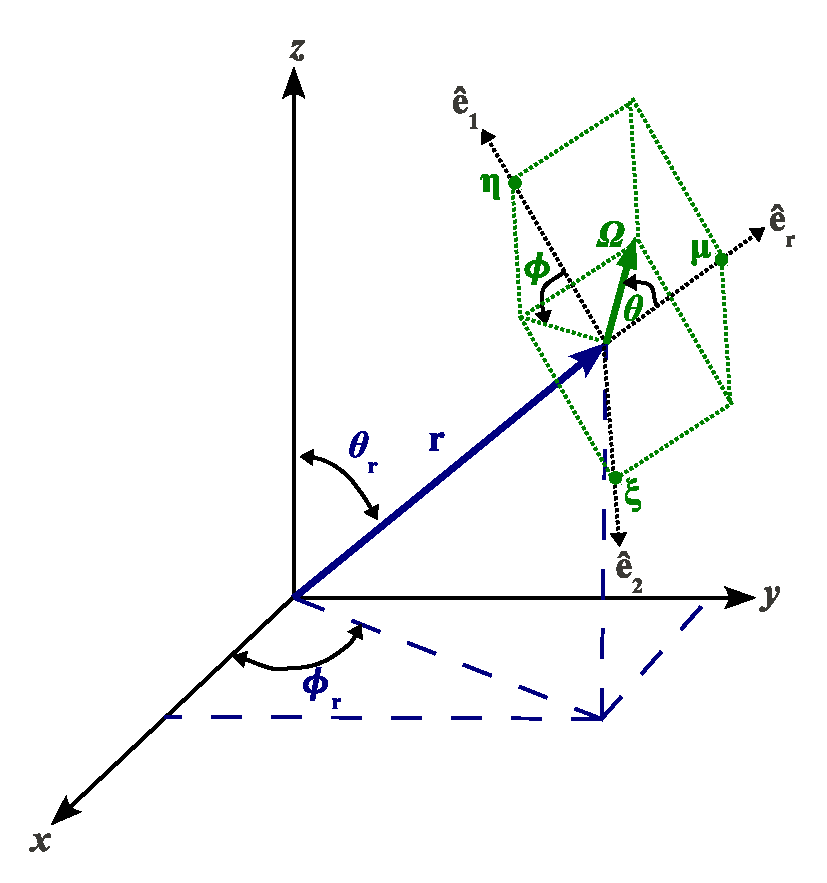
\includegraphics[keepaspectratio, width = 3.0 in]{images/spherical_phase_space}
    \caption{Spherical phase space.}
    \label{fig:spherical_phase_space}
\end{figure}

The streaming operator in spherical coordinates is defined generally as 
\begin{equation}
 \frac{d}{ds} = \frac{dr}{ds}\frac{\partial}{\partial r} + \frac{d\theta_r}{ds}\frac{\partial}{\partial \theta_r} + \frac{d\phi_r}{ds}\frac{\partial}{\partial \phi_r} + \frac{d\mu}{ds}\frac{\partial}{\partial \mu} + \frac{d\phi}{ds}\frac{\partial}{\partial \phi} \, .
\end{equation}
As a simple example, consider the case of 1-d transport in spherical coordinates, for which we assume the flux is independent of the spatial coordinates $\theta_{r}$ and $\phi_{r}$, which eliminates the derivatives with respect to $\theta_r$ and $\phi_r$.  Moreover, if we look at the angular coordinates, we see that if $r$ is the only spatial variable, then there should be dependence only on $\mu$.  A dependence on the azimuthal angle would require a non-uniform particle distribution in the other spatial directions.  Hence, the derivative with respect to $\phi$ also vanishes, leaving
\begin{equation}
 \frac{d}{ds} = \frac{dr}{ds}\frac{\partial}{\partial r} + \frac{d\mu}{ds}\frac{\partial}{\partial \mu}  \, .
\end{equation}
From Figure \ref{fig:spherical_phase_space}, we can immediately see that
\begin{equation}
 \frac{dr}{ds} = \mu \, .
 \label{eq:drds}
\end{equation}
Less obvious is $d\mu/ds$.  First note that $r d\theta = -ds \sin\theta$, which we can see directly from Figure \ref{fig:spherical_angle_with_r}.  The negative sign arises because a positive $ds$ leads to a decrease $\theta$. Then, noting that $\mu = \cos{\theta}$ so that $d\mu = -\sin{\theta} d\theta$, we can show
\begin{equation}
 \frac{d\mu}{ds} = \frac{1-\mu^2}{r} \, ,
 \label{eq:dmuds}
\end{equation}
and
\begin{equation}
 \frac{d\psi}{ds} = \mathbf{\Omega} \cdot \nabla_{\text{1d}} \psi = \mu \frac{\partial \psi}{\partial r} +  \frac{1-\mu^2}{r}\frac{\partial \psi}{\partial \mu} \, .
\end{equation}


\begin{figure}[ht] 
    \centering
    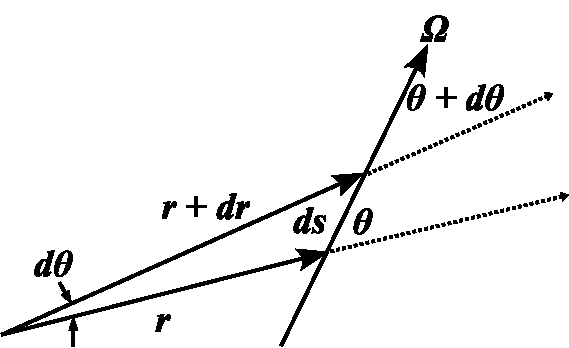
\includegraphics[keepaspectratio, width = 2.5 in]{images/spherical_angle_with_r}
    \caption{Change in $r$ and $\theta$ as a particle streams.}
    \label{fig:spherical_angle_with_r}
\end{figure}


\section*{Example 1: Meandering from a Plane Source in a Vacuum Slab}

As a first example, consider the case of neutrons streaming in a 1-d slab for $x>0$ where the source is an isotropic planar source at $x=0$ which we will use as a boundary condition rather than a source term. The Cartesian streaming term above simplifies in 1-d to
\begin{equation}
 \mu \frac{\partial \psi}{\partial x} = 0 \, ,
\end{equation}
subject to
\begin{equation}
 \psi(0,\mu) = \frac{S_0}{2} \, .
\end{equation}
In 1-d slab geometry, we essentially integrate out the 2$\pi$ associated with the azimuthal angle.  Hence, isotropic sources of strength $S$ become $S/2$ instead of $S/4\pi$.  The units of $\psi$ are slightly different, and one must divide by $2\pi$ [rad] in order to obtain units appropriate in 3-d.  Integrating the equations shows that
\begin{equation}
 \psi(x,\mu) = c \, , \, \, \, \, \mu > 0 \, ,
\end{equation}
for some constant $c$.  At $x = 0$, we must have $\psi(0,\mu) = S/2$, and so for all $x > 0$, $\psi(x,\mu) = S/2$.  The same holds for negative $x$ and $\mu$.

\section*{Example 2: Playing in Vacuum Outside a Spherical Shell Source}

We now consider a neutrons streaming in a vacuum due to an isotropic spherical shell source of radius $r_0$.  We focus only on $r > r_0$.  The transport equation can be written
\begin{equation}
 \mu \frac{\partial \psi}{\partial r} + \frac{1-\mu^2}{r} \frac{\partial \psi}{\partial \mu} = \frac{S_0\delta(r-r_0)}{4\pi r_0} \, .
\end{equation}
From Eqs. \ref{eq:drds} and \ref{eq:dmuds}, we have
\begin{equation}
 ds = \frac{d\mu}{ (1-\mu^2)/r } = \frac{dr}{\mu} \, ,
\end{equation}
or
\begin{equation}
 \frac{dr}{r} = \frac{\mu d\mu}{1-\mu^2} \, .
\end{equation}
We integrate from initial coordinates $r_s$ and $\mu_s$, as shown in Figure \ref{fig:sphere_example}, and rearrange to obtain
\begin{equation}
 \mu = \sqrt{ 1 - (1-\mu^2_s)\Big (\frac{r_s}{r} \Big )^2  } \, .
 \label{eq:angularrestribution}
\end{equation}
\begin{figure}[ht] 
    \centering
    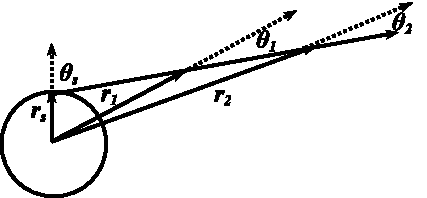
\includegraphics[keepaspectratio, width = 2.5 in]{images/sphere_example}
    \caption{Streaming of particles from spherical shell source.}
    \label{fig:sphere_example}
\end{figure}

Eq. \ref{eq:angularrestribution} shows explicitly how $\mu$ changes as a function of $r$.  This phenomenon is often called angular redistribution and leads to collimation of the flux away from the source.  Since $d\psi/ds$ must equal the source, we can write
\begin{equation}
 ds = \frac{d\mu}{ (1-\mu^2)/r } = \frac{d\psi}{ \frac{S_0\delta(r-r_0)}{4\pi r_0}  } \, ,
\end{equation}
or 
\begin{equation}
\frac{d\psi}{dr} = \frac{S_0\delta(r-r_0)}{4\pi r_0} \, .
\end{equation}
Then
\begin{equation}
 \int^{r,\mu}_{r_s,\mu_s} \frac{d\psi}{dr}  = \int^r_{r_s} dr \frac{S_0\delta(r-r_0)}{4\pi r_0} \, ,
\end{equation}
or
\begin{equation}
 \psi(r,\mu)-\psi(r_s,\mu_s) = \frac{S_0}{8\pi r^2_s} \frac{1}{\sqrt{1-(1-\mu^2_s)}} \, .
\end{equation}
We take the boundary flux to be $\psi(r_s,\mu_s) = 0$, which implies that $\mu_s$ is limited to $\mu_s \leq 0 \leq \pi/2$. If $\mu_s$ spanned through $\pi$, then particles could be born into the sphere and stream out of another location, a complication we care to avoid in this example.  From Eq. \ref{eq:angularrestribution}, we have $(1-\mu^2_s)=(r/r_s)^2(1-\mu^2)$.  We note that for $\mu_s = 0$, $\mu=\sqrt{1-(r_s/r)^2}$ and when $\mu_s=1$, $\mu=1$.  Finally, we have
\begin{equation}
 \psi(r,\mu) = \frac{S_0}{8\pi} \frac{1}{\sqrt{r^2_s - r^2(1-\mu^2)}} \, , \, \, \, \, \, \sqrt{1-\Big ( \frac{r_s}{r} \Big )^2 } \leq \mu \leq 1 \, .
 \label{eq:spherepsi}
\end{equation}

To illustrate the behavior of $\psi$, we have taken $r_s = 1$ and $S_0 = 8\pi$.  Figure \ref{fig:sphere_psi_radius} shows $\psi$ as a function of radius for several $\mu$ values.  Of course, we see that as neutrons move farther from the source, the flux at larger $\theta$ values (smaller $\mu$ values) diminishes, as we expect due to angular redistribution. Figure \ref{fig:sphere_psi_mu} shows $\psi$ as a function of $\mu$ for several values of $r$.  We see effects of the same phenomenon, in that the angular distribution becomes more collimated about $\mu = 1$ for larger $r$.
\begin{figure}[ht] 
    \centering
    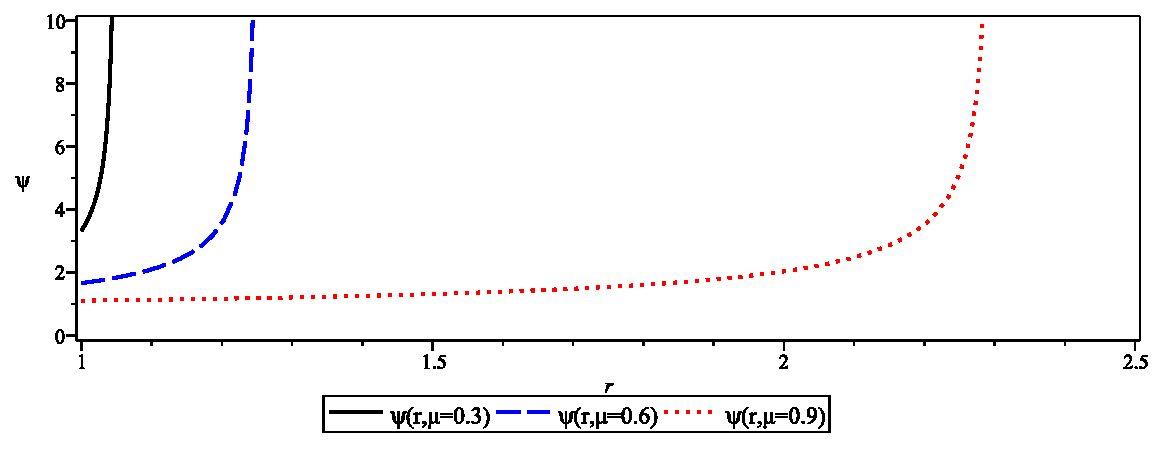
\includegraphics[keepaspectratio, width = 5.0 in]{images/sphere_psi_radius}
    \caption{Angular flux as a function of radius for certain $\mu$ values.}
    \label{fig:sphere_psi_radius}
\end{figure}

\begin{figure}[ht] 
    \centering
    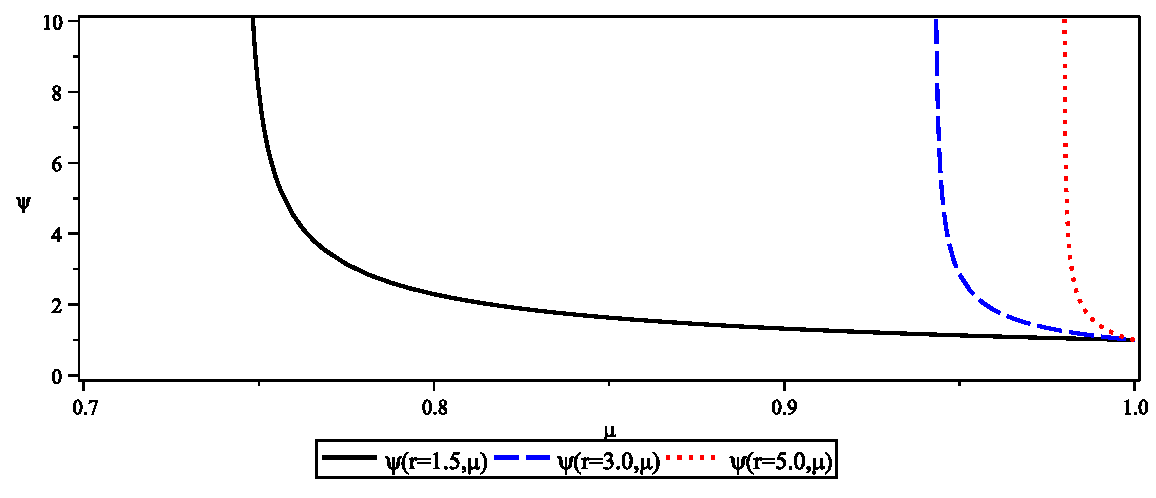
\includegraphics[keepaspectratio, width = 5.0 in]{images/sphere_psi_mu}
    \caption{Angular flux as a function of $\mu$ at certain $r$ values.}
    \label{fig:sphere_psi_mu}
\end{figure}

\section*{Example 3: A Purely Absorbing Slab}

As a final example, we apply what we've learned in vacuum to transport in a purely absorbing slab.  In this case, the 1-d transport equation is
\begin{equation}
 \mu \frac{\partial \psi}{\partial x} + \Sigma_a(x)\psi(x,\mu) = S(x,\mu) \, .
\end{equation}
As an example, we study a uniform slab of length $L$, subject to vacuum boundaries, and with a uniform, isotropic source of volumetric strength\footnote{By volumetric strength, we mean the units are neutrons per unit volume per second.} $S_0$.  Our equation simplifies to 
\begin{equation}
 \mu \frac{\partial \psi}{\partial x} + \Sigma_a \psi(x,\mu) = \frac{S_0}{2} \, .
 \label{eq:slababsorber}
\end{equation}
To solve the problem, we decompose $\psi$ into $\psi_+$ for $\mu > 0$ and $\psi_-$ for $\mu < 0$.  In this way, we can start at one end of the slab and work our way across, essentially as would a neutron.

For $\mu>0$, we divide Eq. \ref{eq:slababsorber} through by $\mu$ and compute the integrating factor
\begin{equation}
 if = \exp{\int^x_0 dx \Sigma_a\mu} = \exp{\Sigma_a x/\mu} \, .
\end{equation}
Then we have
\begin{equation}
 \frac{d}{dx}\Big ( \psi_{+} e^{\Sigma_a x} \Big ) = \frac{S_0}{2\mu}  e^{\Sigma_a x/\mu} \, ,
\end{equation}
and integrating from $0$ to $x$ yields
\begin{equation}
 \psi_{+} = \frac{S_0}{2\Sigma_a}\Bigg (1 - e^{-\Sigma_a x/\mu} \Bigg ) \, ,
\end{equation}
where we note $\psi_+{0,\mu} = 0$ from the given boundary condition.

For $\mu<0$, we do similarly.  It helps in this case to use $-|\mu|$ in place of $\mu$, as it can be easy to lose negative signs.  Using the integrating factor $\exp{(L-x)/|\mu|}$, we find after integrating from $L$ to $x$ that
\begin{equation}
 \psi_{-} = \frac{S_0}{2\Sigma_a}\Bigg (1 - e^{-\Sigma_a (L-x)/|\mu|} \Bigg ) \, .
\end{equation}
For the case of $L = 10$ and $\Sigma_a = 1$, Figure \ref{fig:slab_example_psi} shows $\psi$ for several values of $\psi$.  Note the symmetry, as should be expected. 

\begin{figure}[ht] 
    \centering
    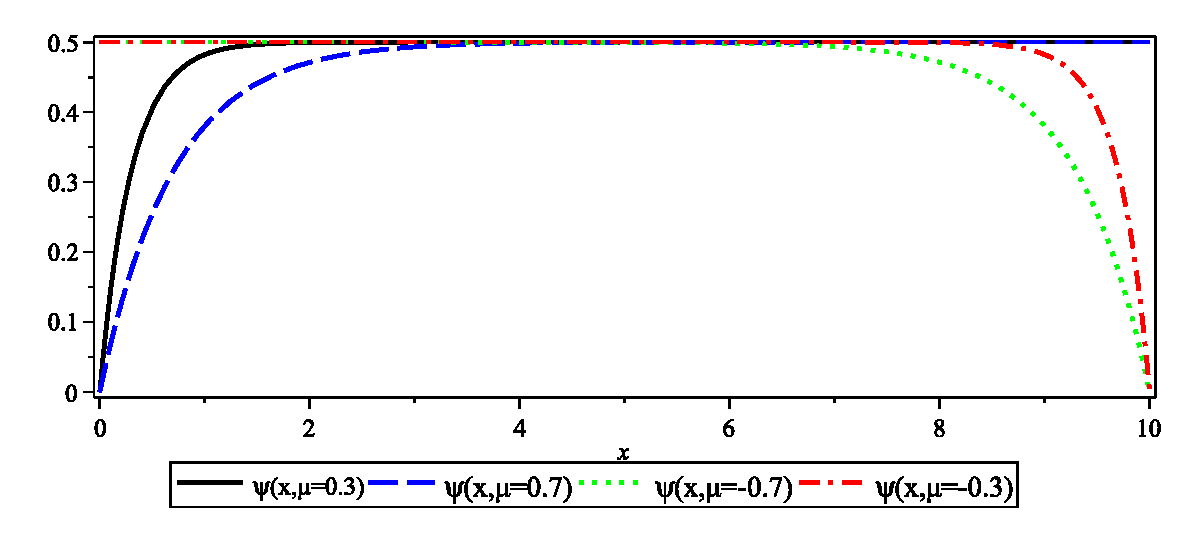
\includegraphics[keepaspectratio, width = 5.0 in]{images/slab_example_psi}
    \caption{Angular flux at specific angles for the absorbing slab.}
    \label{fig:slab_example_psi}
\end{figure}

Our next goal is to compute the scalar flux.  By definition, the scalar flux in 1-d is
\begin{equation}
 \phi(x) = \int^1_{-1} d\mu \psi(x,\mu) \, ,
\end{equation}
which can be broken into
\begin{equation}
  \phi(x) = \int^0_{-1} d\mu \psi_{-}(x,\mu) + \int^1_{0} d\mu \psi_{+}(x,\mu) \, .
\end{equation}
Inserting our expressions above, we have
\begin{equation}
\begin{split}
  \phi(x) &= \frac{S_0}{2\Sigma_a} \Bigg (  \int^{1}_{-1} d\mu - \int^0_{-1} d\mu  e^{-\Sigma_a (L-x)/|\mu|} - \int^1_{0} d\mu e^{-\Sigma_a x/\mu}  \Bigg ) \\
          &= \frac{S_0}{2\Sigma_a} \Bigg ( 2 - \int^1_{0} d\mu'  e^{-\Sigma_a (L-x)/\mu} - \int^1_{0} d\mu e^{-\Sigma_a x/\mu}  \Bigg ) \\
          &= \frac{S_0}{2\Sigma_a} \Bigg ( 2 - E_2(\Sigma_a (L-x)) - E_2(\Sigma_a x)  \Bigg ) \, .
\end{split}
\end{equation}
For the same numerical example, $\phi(x)$ is shown in Figure \ref{fig:slab_example_phi_current} along with the current density $\mathbf{J}(x)$, computation of which is left as an exercise.

\begin{figure}[ht] 
    \centering
    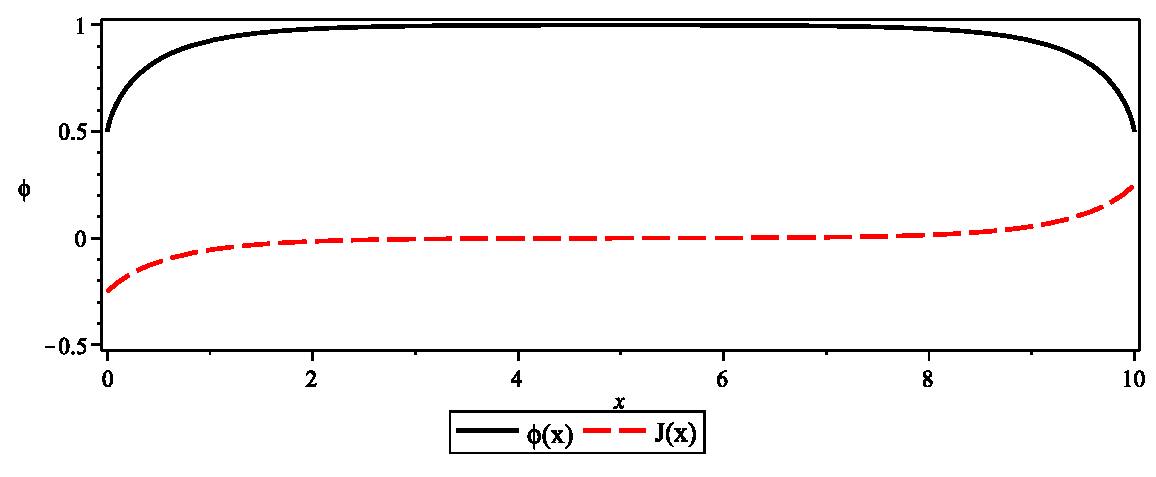
\includegraphics[keepaspectratio, width = 5.0 in]{images/slab_example_phi_current}
    \caption{Scalar flux and current density.}
    \label{fig:slab_example_phi_current}
\end{figure}

\section*{Exponential Integrals}

The functions $E_n(x)$ are called ``exponential integrals'' and are characteristic of slab problems.  They are defined by
\begin{equation}
 E_n(x) \equiv \int^1_0 d\mu \mu^{n-2} e^{-x/\mu} \, .
 \label{eq:EnDefinition}
\end{equation}
They also satisfy
\begin{equation}
 E_n(x) = - \int dx E_{n-1}(x) \, .
 \label{eq:EnIntegration}
\end{equation}
Several of the $E_n$ functions are shown in Figure \ref{fig:slab_example_exp_functions}.

\begin{figure}[ht] 
    \centering
    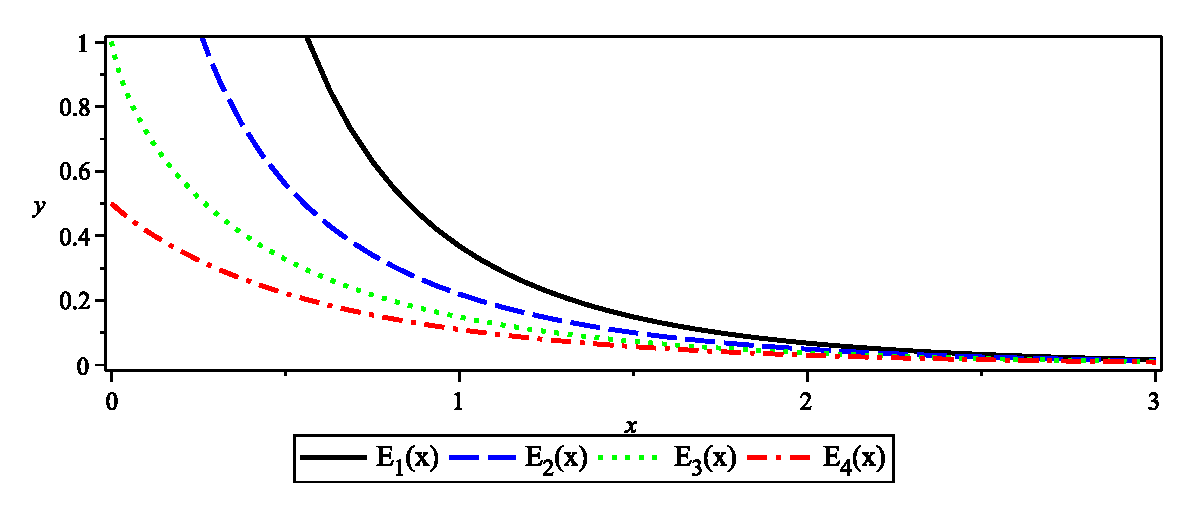
\includegraphics[keepaspectratio, width = 5.0 in]{images/slab_example_exp_functions}
    \caption{The first four exponential integral functions.}
    \label{fig:slab_example_exp_functions}
\end{figure}

\section*{Further Reading}

The problems discussed in this lecture have been rather elementary in nature.  To explore more realistic problems---even just including scattering in slab geometry---would take us into a much more complicated mathematical domain involving integral transforms (with inverses using complex analysis), singular eigenfunction expansions, and more.  Duderstadt and Martin \cite{duderstadt1976tt} cover most of what has been discussed, and much more.  The motivated student should look to that work (specifically Chapter 2), along with Bell and Glasstone (Chapter 2), Case and Zweifel \cite{case1967ltt}, and Davison \cite{davison1957ntt}.  These are listed in reverse chronological order, and perhaps, in increasing order of difficulty.  Davison in particular uses older notation, so the reader be aware!

\begin{exercises}

  \item \textbf{Cylindrical Coordinates}. Derive the streaming term for the neutron transport equation in 1-d cylindrical geometry.  Include diagrams to help explain your approach.
  
  \item \textbf{Angular Current from Plane Source}. In Example 1, what is the angular current $\mathbf{j}$?

  \item \textbf{Isotropic Current Conditions}. For Example 1, find $\psi$ and $\mathbf{j}$ when the boundary condition is an isotropic angular current (rather than an isotropic angular flux).

  \item \textbf{Flux Inside a Sphere}. Solve for the angular flux on the interior of the spherical shell from Example 2.

  \item \textbf{Angular Redistribution in 1-d}. Explain in your own words why $\psi$ in a 1-d spherical problem depends only on the radius $r$ and cosine of the polar angle $\mu$.  Specifically, why is there no dependence on a second angular variable? 

  \item \textbf{Scalar Flux from Spherical Shell Source}. Solve for the scalar flux on the outside of the sphere in Example 2, i.e. integrate Eq. \ref{eq:spherepsi} over $\mu$.  What happens at $r = r_s$ and why?  What is the limiting behavior of $\phi(r)$ as $r\to \infty$?  In other words, what does the spherical source ``look like'' far from its surface?

  \item \textbf{Current Density in a Slab}. Derive an expression for the current density $\mathbf{J}$ for a purely absorbing slab.  Using the values from the example, generate the curves in Figure \ref{fig:slab_example_phi_current}.  Compute the total absorption rate in the slab and the leakage rate at the boundaries.  Is it what you expect?

\end{exercises}

\chapter{The Integral Form}

In this lecture we consider the integral form of the transport equation in both general coordinates and the specific case of slab geometry.  The integral form is useful in situations where only the scalar flux is required and is the foundation for the collision probabability method, which we cover in the next lecture, as well as the method of characteristics, fast becoming the technique of choice in reactor analysis.  We consider some analytical aspects of the integral equation and finish by discussing a simple numerical approach based on Neumann series expansions.

\section*{The Integral Transport Equation}

You may have noticed from the previous two lectures that the angular dependence of the particle density is a relatively unique aspect of transport processes.  Often, this angular dependence is the hardest aspect that we deal with directly, either analytically or numerically\footnote{Energy is by far more complex, as we've noted, and there are very few analytical problems where energy can be handled directly (slowing down in an infinite homogeneous medium problem is one example). Consequently, we typically use only the crudest representation possible in discretizing the energy variable, though much physics goes into generating the discrete data.}  It would be nice to eliminate the angular variable completely, and for certain problems, the \textit{ integral transport equation} allows us to do with a minimum of approximation.

Before we derive the integral form of the transport equation, it helps define a new quantity called the \textit{emission density},
\begin{equation}
  Q(\mathbf{r},\mathbf{\Omega}) = \int_{4\pi} d\Omega' \Sigma_s(\mathbf{r},\mathbf{\Omega}\cdot\mathbf{\Omega}')\psi(\mathbf{r},\mathbf{\Omega'}) + S(\mathbf{r},\mathbf{\Omega}) \, .
  \label{eq:emissiondensity}
\end{equation}
Essentially, $Q$ is a generalized source containing any external source $S$ and scattering source; of course, fission could also be included.

Recall the discussion of Eq. \ref{eq:spaceratepsi}, where we consider a distance $s$ from some reference point $\mathbf{r}_0$ along the characteristic $\mathbf{r}_0 +s\mathbf{\Omega}$.  The full transport equation in terms of $s$ is 
\begin{equation}
    \frac{d}{ds} \psi(\mathbf{r}_0 +s\mathbf{\Omega},\mathbf{\Omega}) + \Sigma_t(\mathbf{r}_0 +s\mathbf{\Omega})\psi =   Q(\mathbf{r}_0 +s\mathbf{\Omega},\mathbf{\Omega})  \, ,
    \label{eq:forchareq}
\end{equation}
which can be called the \textit{forward characteristic} equation, as we follow neutrons forward from the reference point.  Similar, and which we use below, is the \textit{backward characteristic} form, which represents following neutrons backward along the characteristic from a current point $\mathbf{r}$.  Let $p = -s$.  Then $d/dp = -d/ds$ and Eq. \ref{eq:forchareq} becomes (after dropping the $0$ subscript from $\mathbf{r}$)
\begin{equation}
    -\frac{d}{dp} \psi(\mathbf{r} - p\mathbf{\Omega},\mathbf{\Omega}) + \Sigma_t(\mathbf{r} -p\mathbf{\Omega})\psi =   Q(\mathbf{r} -p\mathbf{\Omega},\mathbf{\Omega})  \, .
    \label{eq:backchareq}
\end{equation}
We wish to integrate from $p=0$ to some maximum distance (eventually to be either infinity or a global boundary).  Introducing the integrating factor
\begin{equation}
 if = e^{ -\int^p_0 \Sigma_t(\mathbf{r} -p'\mathbf{\Omega}) dp'  } \, 
\end{equation}
into Eq. \ref{eq:backchareq}, we have
\begin{equation}
    -\frac{d}{dp} \Big ( \psi(\mathbf{r}_0 - p\mathbf{\Omega},\mathbf{\Omega}) e^{ -\int^p_0 \Sigma_t(\mathbf{r} -p'\mathbf{\Omega}) dp'  } \Big ) =  Q(\mathbf{r} -p\mathbf{\Omega}) e^{ -\int^p_0 \Sigma_t(\mathbf{r} -p'\mathbf{\Omega}) dp'  } \, ,
\end{equation}
and integrating
\begin{equation}
  \begin{split}
    -\int^{\psi(p'=p)}_{\psi(p=0)}  \Bigg(  d \Big ( \psi(\mathbf{r} &- p'\mathbf{\Omega},\mathbf{\Omega})   e^{ -\int^{p'}_0 \Sigma_t(\mathbf{r} -p''\mathbf{\Omega}) dp''  } \Big ) \Bigg ) = \\
   & \int^p_0 Q(\mathbf{r} -p'\mathbf{\Omega},\mathbf{\Omega})e^{ -\int^{p'}_0 \Sigma_t(\mathbf{r} -p''\mathbf{\Omega}) dp''  }dp'   \\
  \end{split}
\end{equation}
yields
\begin{equation}
  \begin{split}
    \psi(\mathbf{r},\mathbf{\Omega}) - \psi(\mathbf{r} &- p\mathbf{\Omega},\mathbf{\Omega})e^{ -\int^{p}_0 \Sigma_t(\mathbf{r} -p''\mathbf{\Omega}) dp''  }  = \\
   & \int^p_0 Q(\mathbf{r} -p'\mathbf{\Omega},\mathbf{\Omega})e^{ -\int^{p'}_0 \Sigma_t(\mathbf{r} -p''\mathbf{\Omega}) dp''  }dp'   \, .
  \end{split}
\end{equation}

We can simplify the notation somewhat by defining the \textit{optical pathlength} $\tau$, such that
\begin{equation}
  \tau ( \mathbf{r} ,\mathbf{r} -p \mathbf{\Omega} ) = \int^p_0 \Sigma_t(\mathbf{r} -p'\mathbf{\Omega}) dp' \, . 
  \label{eq:opticalpathlength}
\end{equation}
Then, the integral equation for the angular flux becomes
\begin{equation}
  \begin{split}
    \psi(\mathbf{r},\mathbf{\Omega}) = \int^p_0 Q(\mathbf{r} -p'\mathbf{\Omega},\mathbf{\Omega})e^{-\tau(\mathbf{r},\mathbf{r}-p'\mathbf{\Omega})}dp'                         +  \psi(\mathbf{r} - p\mathbf{\Omega},\mathbf{\Omega})e^{ -\tau(\mathbf{r},\mathbf{r}-p\mathbf{\Omega}) }   \, .
  \end{split}
  \label{eq:inteqpsi}
\end{equation}

In many cases, the emission density $Q$ is assumed to be isotropic in the lab system.  In this case, we can integrate out the angular dependence and arrive at an integral equation for the scalar flux often referred to as Peierl's equation.  To do so, we let the integration bound $p$ of Eq. \ref{eq:inteqpsi} go to infinity.  We assume the second term on the right hand side to vanish (i.e. either $\psi$ vanishes at infinity, or equivalently, the optical path length $\tau(\mathbf{r},\infty)$ goes to $\infty$, and so the exponential vanishes).  

Letting $Q(\mathbf{r},\mathbf{\Omega}) = Q(\mathbf{r} -p\mathbf{\Omega})/4\pi$, and substituting $\mathbf{r}' = \mathbf{r} - p \mathbf{\Omega}$, we integrate Eq. \ref{eq:inteqpsi} over all angles to get
\begin{equation}
 \phi(\mathbf{r}) = \int_{4\pi} d\Omega \int^{\infty}_0  \frac{Q(\mathbf{r}')}{4\pi}e^{-\tau(\mathbf{r},\mathbf{r}')}dp \, .
 \label{eq:integralphiPRE}
\end{equation}
Now note that $p =|\mathbf{\Omega} p|=|\mathbf{r}-\mathbf{r}'|$, and consequently $p^2 = |\mathbf{r}-\mathbf{r}'|^2$.  Multiplying within the integrand by $1=p^2/|\mathbf{r}-\mathbf{r}'|^2$ yields
\begin{equation}
 \phi(\mathbf{r}) = \int_{4\pi} d\Omega \int^{\infty}_0  \frac{Q(\mathbf{r}')}{4\pi}e^{-\tau(\mathbf{r},\mathbf{r}')}\frac{p^2dp}{|\mathbf{r}-\mathbf{r}'|^2} \, ,
\end{equation}
and if the reader thinks this looks suspiciously like a volume integral in spherical coordinates, she would be right.  Letting $dV' = 4\pi d\Omega dpp^2$, we have
\begin{equation}
 \phi(\mathbf{r}) = \int_{V'} \frac{ Q(\mathbf{r}')e^{-\tau(\mathbf{r},\mathbf{r}')} dV'}{4\pi|\mathbf{r}-\mathbf{r}'|^2} \, .
 \label{eq:integralphi}
\end{equation}

\section*{Integral Transport in Slab Geometry}

We now look at the special case of Eq. \ref{eq:integralphi} in slab geometry, for which the emission density is a function only of $x$, i.e. $Q(\mathbf{r}) = Q(x)$.  We make use of cylindrical coordinates, with the axis taken to be $x$.  Our goal will be to integrate out the radial ($\rho$) and azimuthal ($\omega$) spatial components, leaving just the $x$ dependence. The differential volume is then
\begin{equation}
 dV' = \rho d\rho d\omega dx' ,
\end{equation}
and Eq. \ref{eq:integralphi} becomes
\begin{equation}
\begin{split}
 \phi(x) &= \int^{\infty}_{-\infty} dx' \int^{\infty}_0 d\rho \rho \int^{2\pi}_0 \frac{ d\omega' Q(x')e^{-\tau(\mathbf{r},\mathbf{r}')}}{4\pi|\mathbf{r}-\mathbf{r}'|^2} \, \\
        &= 2\pi \int^{\infty}_{-\infty}dx' \int^{\infty}_0 d\rho \rho \frac{ Q(x')e^{-\tau(\mathbf{r},\mathbf{r}')}}{4\pi |\mathbf{r}-\mathbf{r}'|^2} \, .
\end{split}
\label{eq:integralphix}
\end{equation}

We now need to express $\mathbf{r}$ and $\rho$ in terms of $x$.  Since the cross-sections (as quantified by $\tau$) are really dependent only on $x$, we can relate the full distance $|\mathbf{r}' - \mathbf{r}|$ with its projection along the $x$ axis via a directional cosine $\lambda^{-1}$ such that
\begin{equation}
 \lambda = \frac{|\mathbf{r}' - \mathbf{r}|}{|x'-x|} \, 
 \label{eq:projection}
\end{equation}
and $\tau(\mathbf{r}',\mathbf{r}) = \lambda \tau(x',x)$.  Moreover,
\begin{equation}
 |\mathbf{r}' - \mathbf{r}|^2 = \rho^2 + |x' - x|^2 \, 
\end{equation}
which, using Eq. \ref{eq:projection}, can be rewritten as
\begin{equation}
 \rho^2 = (\lambda^2 -1 )|x'-x|^2 \, ,
\end{equation}
and differentiating, we find
\begin{equation}
 \rho d\rho = \lambda d\lambda |x'-x|^2 \, .
\end{equation}
Noting that $\rho = 0$ corresponds to $\lambda = 1$, Eq. \ref{eq:integralphix} can be written in terms of $\lambda$ to give
\begin{equation}
\begin{split}
 \phi(x) &= 2\pi \int^{\infty}_{-\infty}dx' \int^{\infty}_1 \lambda d\lambda \frac{|x'-x|^2 }{4\pi|\mathbf{r}' - \mathbf{r}|^2}    Q(x')e^{-\tau(\mathbf{x},\mathbf{x}')} \\
        &= 2\pi \int^{\infty}_{-\infty}dx' \int^{\infty}_1 \lambda d\lambda \frac{1}{4\pi \lambda^2}    Q(x')e^{-\tau(\mathbf{x},\mathbf{x}')} \\       
        &=  \int^{\infty}_{-\infty} dx'\frac{1}{2} \int^{\infty}_1 \lambda d\lambda\frac{1}{\lambda}  Q(x')e^{-\tau(\mathbf{x},\mathbf{x}')} \, 
\end{split}
\end{equation}
or
\begin{equation}
 \phi(x) =  \int^{\infty}_{-\infty} dx'\frac{1}{2} E_1(\tau(\mathbf{x},\mathbf{x}'))Q(x') \, ,   
 \label{eq:integralphislab}     
\end{equation}
where we have used the $E_1$ function defined at the end of Lecture \ref{lec:analytical}.  

\section*{First-Flight Kernels}

Eq. \ref{eq:integralphislab} gives us an example of the use of a \textit{first-flight kernel} for the scalar flux, the general use of which takes the form
\begin{equation}
 \phi(\mathbf{r}) = \int d^3\mathbf{r}' k(\mathbf{r},\mathbf{r}')Q(\mathbf{r}') \, 
\end{equation}
for a kernel $k(\mathbf{r},\mathbf{r'})$.  For slab geometry, the first-flight kernel is seen to be
\begin{equation}
 k_{\text{slab}}(x,x') = \frac{1}{2} E_1(\tau(x,x')) \, .
 \label{eq:firstflightkernelslab}
\end{equation}

First-flight kernels have a particularly easy (and important!) physical interpretation. Consider Eq. \ref{eq:integralphislab} for the case of a purely absorbing medium.  Then the emissivity $Q$ consists only of external sources.  To help visualize the problem, take $Q$ to be a delta function at $x_0$, i.e. $Q(x) = Q_0 \delta(x-x_0)$.  Substituting this into Eq. \ref{eq:integralphislab} gives
\begin{equation}
 \phi(x) = \frac{1}{2} E_1(\tau(x,x_0)) Q_0 \, . 
\end{equation}
Thus, the kernel $k(x,x')$ can be seen to give the contribution of the source particles born at $x'$ to the flux at $x$.  In other words, it gives to us the \textit{uncollided flux}.  For many systems, having the uncollided flux can be a good approximation for the total flux, and in some numerical schemes, it can be a good initial guess to help reduce computational time and numerical artifacts (e.g. the discrete ordinates method, discussed in Lecture \ref{lec:discreteordinates}).

If we look back at the Peierl's equation (Eq. \ref{eq:integralphi}), we find the fundamental first-flight kernel of the point source, 
\begin{equation}
 k_{\text{point}}(\mathbf{r},\mathbf{r}') = \frac{e^{-\tau(\mathbf{r},\mathbf{r}')}}{4\pi|\mathbf{r}-\mathbf{r}'|^2} \, .
 \label{eq:firstflighkernelpoint}
\end{equation}

Two things are worth noting about Eq. \ref{eq:firstflighkernelpoint}.  First, the first-flight kernels for all other geometrical configurations can be derived from this kernel.  A second point, related to the first, is that the point kernel is closely related to the \textit{Green's function} for the transport equation.  

\section*{Green's Functions}


A Green's function $G(x,x')$ for a linear differential operator\footnote{We'll discuss the linearity of the transport equation in Lecture \ref{lec:linearity}, and we'll use operator notation extensively in Lecture \ref{lec:adjoint}.} $L=L(x)$ is defined
\begin{equation}
 LG(x,x') = \delta(x-x') \, .
 \label{eq:greens}
\end{equation}
A linear differential operator is any linear combination of basic differentiation operators.  $L$ could be $d/dx$ or $d^2/dx^2$ or $d^2/dx^2 + d/dx$, and so on.  The utility of $G$ arises when we wish to solve the inhomogeneous differential equation
\begin{equation}
 Lu(x) = f(x) \, .
 \label{eq:diffeq}
\end{equation}
If we multiply both sides of Eq. \ref{eq:greens} by $f(x')$ and integrate over $x'$, we find
\begin{equation}
 \int LG(x,x')f(x')dx' = \int dx' \delta(x-x') f(x') = f(x) \, ,
\end{equation}
but this suggests that
\begin{equation}
 Lu(x) = \int LG(x,x')f(x')dx' = L \int G(x,x')f(x')dx'  \, ,
\end{equation}
or 
\begin{equation}
 u(x) = \int G(x,x')f(x')dx'  \, .
\end{equation}
Hence, if we know $G(x,x')$, then we can solve the inhomogeneous equation for $u$.  

What about the transport equation?  Consider again Eq. \ref{eq:inteqpsi}, neglecting the second term, and letting $p\to \infty$, i.e. 
\begin{equation}
  \begin{split}
    \psi(\mathbf{r},\mathbf{\Omega}) = \int^{\infty}_0 Q(\mathbf{r} -p\mathbf{\Omega},\mathbf{\Omega})e^{-\tau(\mathbf{r},\mathbf{r}-p\mathbf{\Omega})}dp                          \, .
  \end{split}
  \label{eq:inteqpsi2}
\end{equation}
Note that this is still integrating along the characteristic.  It is more convenient to cast this as volume integral, similar to what we did above for Eq. \ref{eq:integralphi}.  However, even in volume form, we still want the integration confined to the characteristic.  By defining
\begin{equation}
 \delta(\mathbf{\Omega}\cdot\mathbf{\Omega}') \equiv \delta(\mu-\mu')\delta(\phi-\phi') \, ,
\end{equation}
and
\begin{equation}
 \mathbf{\Omega}_R \equiv \frac{\mathbf{r} -\mathbf{r}'}{|\mathbf{r}-\mathbf{r}'|} \, ,
\end{equation}
and recalling $p = |\mathbf{r}-\mathbf{r}'|$, we can rewrite Eq. \ref{eq:inteqpsi2} as
\begin{equation}
    \psi(\mathbf{r},\mathbf{\Omega}) = \int_{4\pi} d\Omega_R \delta(\mathbf{\Omega}\cdot\mathbf{\Omega}_R) \int^{\infty}_0 Q(\mathbf{r}',\mathbf{\Omega}_R)e^{-\tau(\mathbf{r},\mathbf{r'})}dp                          \, .
\end{equation}
Using $dV' = p^2dpd\Omega_R$, this becomes
\begin{equation}
    \psi(\mathbf{r},\mathbf{\Omega}) = \int_{V'} dV' \frac{1}{|\mathbf{r}-\mathbf{r}'|^2} \delta(\mathbf{\Omega}\cdot\mathbf{\Omega}_R)  Q(\mathbf{r}',\mathbf{\Omega}_R)e^{-\tau(\mathbf{r},\mathbf{r'})}                          \, .
\end{equation}

Now let $Q$ be a delta source at $\mathbf{r}_0$ emitting particles in direction $\mathbf{\Omega}_0$, or  $Q = \delta(\mathbf{r}-\mathbf{r}_0)\delta(\Omega\cdot\Omega_0)$, similar to the right hand side of Eq. \ref{eq:greens}. Then
\begin{equation}
  \begin{split}
    \psi(\mathbf{r},\mathbf{\Omega}) &= \int_{V'} dV' \frac{e^{-\tau(\mathbf{r},\mathbf{r'})} }{|\mathbf{r}-\mathbf{r}'|^2} \delta(\mathbf{\Omega}\cdot\mathbf{\Omega}_R) \delta(\mathbf{r}-\mathbf{r}_0)\delta(\mathbf{\Omega}\cdot\mathbf{\Omega}_0)                           \\
    &= \frac{e^{-\tau(\mathbf{r},\mathbf{r}_0)} }{|\mathbf{r}-\mathbf{r}_0|^2} \delta \Bigg (\mathbf{\Omega}\cdot \frac{\mathbf{r} -\mathbf{r}_0}{|\mathbf{r}-\mathbf{r}_0|} \Bigg ) \delta(\mathbf{\Omega}\cdot\mathbf{\Omega}_0) \\
    &= G_{\text{point}}(\mathbf{r},\mathbf{\Omega};\mathbf{r}_0,\mathbf{\Omega}_0) \, .
  \end{split}
  \label{eq:psigreen}
\end{equation}
This is the Green's function for the angular flux, with which we can find $\psi$ for any emission density $Q(\mathbf{r},\mathbf{\Omega}$)\footnote{Careful! If $Q$ includes scattering, then it depends on $\psi$, and so a direct solution in this form is not possible}.   We can use $G_{\text{point}}$ to recover the scalar flux point kernel by letting $Q$ be a unit isotropic point source, i.e. $Q = \delta(\mathbf{r}-\mathbf{r}_0)/4\pi$.  Then
\begin{equation}
\begin{split}
    \psi(\mathbf{r},\mathbf{\Omega}) &=  \int_V dV' \int_{4\pi} d\Omega' G_{\text{point}}(\mathbf{r},\mathbf{\Omega};\mathbf{r}',\mathbf{\Omega}') \frac{\delta(\mathbf{r}'-\mathbf{r}_0)}{4\pi} \\
    &= \frac{e^{-\tau(\mathbf{r},\mathbf{r}_0)} }{4\pi|\mathbf{r}-\mathbf{r}_0|^2} \delta \Bigg (\mathbf{\Omega}\cdot \frac{\mathbf{r} -\mathbf{r}_0}{|\mathbf{r}-\mathbf{r}_0|} \Bigg ) \, .
\end{split}
\label{eq:psiisosource}
\end{equation}
Integrating $\psi$ over all angles yields
\begin{equation}
\begin{split}
    \phi(\mathbf{r}) &=  \int_{4\pi} d\Omega \frac{e^{-\tau(\mathbf{r},\mathbf{r}_0)} }{4\pi|\mathbf{r}-\mathbf{r}_0|^2} \delta \Bigg (\mathbf{\Omega}\cdot \frac{\mathbf{r} -\mathbf{r}_0}{|\mathbf{r}-\mathbf{r}_0|} \Bigg ) \\
    &= \frac{e^{-\tau(\mathbf{r},\mathbf{r}_0)} }{4\pi|\mathbf{r}-\mathbf{r}_0|^2} \, ,
\end{split}
\end{equation}
which is indeed our point kernel for the scalar flux.

\section*{Neumann Series}

Lecture \ref{lec:cpm} will cover the widely-used collision probability method that is based on the integral transport equation.  Here, we investigate a less versatile yet quite enlightening method based on expansion of the scalar flux in a so-called Neumann\footnote{Carl Neumann, not to be confused with John von Neumann.} series for slab problems that include scattering.

Consider the integral equation in a slab of length $L$:
\begin{equation}
 \phi(x) = \int^L_0  dx' \frac{1}{2} E_1(\tau(x,x'))(S(x') + \phi(x')\Sigma_s(x')) \, .
\end{equation}
Defining the operator $K$,
\begin{equation}
 K\phi = \int^L_0  dx' \frac{1}{2} E_1(\tau(x,x'))\phi(x) \Sigma_s(x) \, ,
\end{equation}
we can rewrite the integral equation as
\begin{equation}
 (I-K)\phi = K\frac{S}{\Sigma_s} \, .
 \label{eq:integraloperatorform}
\end{equation}
Without going into formal detail (though it should seem ``reasonable''), Eq. \ref{eq:integraloperatorform} can be solved by expanding
\begin{equation}
 (I-K)^{-1} = I + K + K^2 + \ldots \, ,
\end{equation}
where $I$ is the identity operator, so that 
\begin{equation}
 \phi(x) = \sum^{\infty}_{n=0} K^n \frac{S(x)}{\Sigma_s(x)} \, .
 \label{eq:neumannseries}
\end{equation}

Suppose we define
\begin{equation}
 \phi_n(x) \equiv K^n \frac{S(x)}{\Sigma_s(x)} \, .
\end{equation}
Then we see that $\phi_0 = K(S/\Sigma_s)$, $\phi_1 = K^2(S/\Sigma_s) = K(\phi_0)$ and so on.  We recognize $\phi_0(x)$ as the uncollided flux, which is then used as input for $\phi_1$.  We recognize $\phi_1$ as those neutrons already having undergone a single collision (and no more).  In general, we call $\phi_n$ the $n$th collided flux.  The Neumann series Eq. \ref{eq:neumannseries} just adds up all neutrons that have not collided, those that have collided once, those that have twice, and so on, thus capturing the entire population of neutrons in the system.  Defining (and computing)  $\phi_n$ in terms of the previous term $\phi_{n-1}$ sequence is called \textit{Neumann iteration}.

\section*{A Numerical Example}

We illustrate the use of Neumann iteration in a simple MATLAB code for a homogeneous slab problem with a uniform isotropic source.  The integrals involved are approximated using the trapezoid rule, though the exercises explore other schemes.  Please refer to the code comments in Listing \ref{list:neumann_slab} to understand the exact implementation of the algorithm.


\lstset{language=Octave,caption=Solution of Slab Problem via Neumann Series, label=list:neumann_slab}
\lstinputlisting{code/neumann_slab.m}

\section*{Further Reading}

The derivation of the integral equations generally follow that of Lewis and Miller \cite{lewis1993cmn}.  First-flight kernels and Green's functions are covered in Duderstadt and Martin \cite{duderstadt1976tt} and Case and Zweifel \cite{case1967ltt}.  Solving for the scalar flux via Neumann iterations is discussed in Duderstadt and Martin \cite{duderstadt1976tt}, while its use as a general technique for integral equations is described e.g. by Arfken and Weber. Any good numerical analysis textbook will provide more information on numerical integration, and the reader is encouraged to explore this fundamental topic.    

\begin{exercises}
  
  \item \textbf{Point-to-slab}. Show how $k_{\text{slab}}$ can be generated using $k_{\text{point}}$.
  \item \textbf{Line source}. Show that the first-flight kernel for an infinite isotropic line source is given by
        \begin{equation}
         k_{\text{line}}(r,r') = \frac{1}{2\pi r}Ki_1(\Sigma_t|r-r'|) \, ,
         \label{eq:linekernel}
        \end{equation}
        where
        \begin{equation}
         Ki_n(x) = \int^{\pi/2}_0 \cos^{n-1}(\theta) e^{-x/\cos(\theta)}d\theta = \int^{\infty}_0 \frac{e^x \cosh(u)}{\cosh^n(u)} \, 
        \end{equation}
        are the Bickley-Naylor function of order $n$, and where $Ki_0(r) = K_0(r)$, the zeroth order modified Bessel function.

  \item \textbf{Spherical shell}. Show that the first-flight kernel for a spherical shell is given by
        \begin{equation}
         k_{\text{sph}}(r,r') = \frac{r'}{2r}Ki_1(\Sigma_t|r-r'|-\Sigma_t|r+r'|) \, ,
         \label{eq:sphericalkernel}
        \end{equation}

  \item \textbf{Current density kernels}. In the lecture found the flux kernel for a plane source, and the kernels for line and spherical sources are given in the first two exercises.  We can also derive kernels for the current density.  For example, in a slab, there is a current kernel $\gamma_{\text{slab}}(x,x')$ such that
  \begin{equation}
   \mathbf{J}(x) = \int^L_0 \gamma_{\text{slab}}(x,x') Q(x') dx' \, .
  \end{equation}
  Derive this kernel $\gamma_{\text{slab}}(x,x')$.
 
  \item \textbf{Using kernels}. Use $k_{\text{slab}}$ to find the scalar flux for the example of Lecture \ref{lec:analytical}, and use $\gamma_{\text{slab}}$ to find the corresponding current density.

  \item  \textbf{Neumann Series}. Use the Neumann series code for the slab in Listing \ref{list:neumann_slab} to plot the scalar flux, uncollided flux, and the first five collided fluxes on the same graph using 20 spatial divisions for $L = 10$, $\Sigma_t = 1.0$, and (a) $\Sigma_s = 0.2$ and (b) $\Sigma_s = 0.8$.  What changes for the case with higher scattering?

  \item \textbf{Convergence}. For the same problem, modify the Neumann series code to compute as many collided fluxes are necessary so that
  \begin{equation*}
   \frac{|\phi_n(x_i)-\phi_n(x_{i-1})|}{\phi_n(x_{i-1}} < \epsilon = 1\times10^{-6} \, \, \, \, \, \, \forall \, x_i \, ,
  \end{equation*}
   and comment on the results. (Hint, which norm on the $x$ vector is appropriate?)
  
  \item \textbf{Nonuniform medium}. Could the Neumann series code be easily modified to handle a nonuniform slab?  Suggest an approach for this.

  \item \textbf{Numerical integration}. Modify the Neuman series code to handle both Simpson's rule and Gaussian quadrature.  Overviews of both can be found in numerical analysis texts.  For the purely absorbing slab example of Lecture \ref{lec:analytical}, compare the trapezoid, Simpson's, and Gaussian schemes to the analytical solution.  Comment on which method appears to get it ``right`` with the least effort.

  \item \textbf{Efficiency}.  The Neumann code is slow due to the symbolic computation of the $E_n$ functions. Modify the code to precomputing the various coefficients (indexed by $i$ and $j$), and comment on any improvement.  For even greater efficiency, find a way to evaluate the exponential functions numerically (via some form of approximation) that allows you compute $E_n(x)$ rapidly; see for example Hebert's \textit{Applied Reactor Physics}.  How does the numerical evaluation affect the accuracy of the result?


\end{exercises}

\chapter{Collision Probability Method}
\label{lec:cpm}

\begin{exercises}
  \item Assume a medium has total macroscopic cross-section $\Sigma$.  Derive the escape probabilities for (a) an infinite slab of width $a$, (b) an infinite cylinder of radius $r$, and (c) a sphere of radius $r$.
\end{exercises}

\chapter{CPM in Cylindrical Coordinates}
\label{lec:cpm_cylinder}

In this lecture, the collision probability method is derived for 
1-D cylindrical coordinates and specialized for the case of 
annular systems.  For many years, this approach was fundamental for 
pin-cell spectrum calculations.

\section*{Sample Code}

To be continued.

\section*{Further Reading}

Lewis and Miller. Hebert.  Carlvik 1964 paper.

%------------------------------------------------------------------------------%
\begin{exercises}

  %----------------------------------------------------------------------------%
  \item \textbf{White Boundary Conditions}. 
  
  Collision probabilities 
  found using the methods discussed in this lecture can be modified to 
  account for white boundary conditions by setting 
  \begin{equation*}
  R_i =  \Sigma_{i}V_i - \sum_{j} \Sigma_j V_j P_{j\to i} \, ,
  \end{equation*}
  and defining updated collision probabilities
  \begin{equation*}
  \Sigma_{i}V_i P^{\text{white}}_{j\to i} = 
    \Sigma_{i}V_i P_{j \to i} - \frac{R_i R_j}{\sum_k R_k} \, .
  \end{equation*}
  Prove this expression by using reciprocity relations.

    
\end{exercises}
%

\chapter{P$\mathrm{_N}$ Method and Diffusion}

\begin{exercises}

  \item  \textbf{P$_{\mathbf{1}}$ Boundary Conditions}. Derive the $P_1$ equations for isotropic scattering and an isotropic source.  Derive the Marshak vacuum conditions for arbitrary left and right boundaries in a slab.  Do the same for the Mark conditions. 

  \item \textbf{P$_{\mathbf{2}}$ Equations}.Show for the case of linearly anisotropic scattering and isotropic source that the $P_2$ equations can be written as a second order partial differential equation similar in form to the typical neutron diffusion equation.

  \item \textbf{Numerical Solution of the P$_{\mathbf{1}}$ Equations}. Consider a slab of width 10 cm with $\Sigma_t = 1.0$ [cm$^{-1}$], and $c = \Sigma_s / \Sigma_t = 0.5$ (isotropic scattering in the lab system).  A uniform, isotropic source of $1$ [n/cm$^2$-s] is located in the first half of the slab, and both slab edges are subject to vacuum conditions. Write a code to solve the $P_1$ approximation to this problem using Marshak conditions.  Plot $\psi(x,\mu)$ at $x = 0$, $2.5$, $5.0$, $7.5$, and $10$ [cm].  Plot $\phi(x)$ over the whole slab.

  \item \textbf{Numerical Solution of the P$_{\mathbf{3}}$ Equations}. For the same problem, write a code to solve the $P_3$ approximation using Marshak conditions.

  \item \textbf{ Diffusion via asymptotics}.  Consider the following rescaling of the 1-d, mono-energetic transport equation with isotropic scattering. Finish me.

  \item \textbf{Legendre Addition Theorem}. Prove the Legendre polynomial addition theorem.  You may use any resource you want, but make sure you understand all steps of the proof.  A particularly straightforward approach begins as follows.  Start with an expansion of an arbitrary function in the full spherical harmonics.  Then, substitute the definition of the expansion coefficients back into the expansion.  Noting that the integral and summation can be switched, what function must the summation be?  

  \item \textbf{Defining the Scattering Angle}. Prove $\mu_0 = \cos(\theta)\cos(\theta')+\sin(\theta)\sin(\theta')\cos(\phi-\phi')$, where $\mu_0$ is the cosine of the scattering angle and ($\theta$,$\phi$) and $(\theta',\phi')$ are the original and final angles, respectively.  Include a diagram.

\end{exercises}

\chapter{Numerical Diffusion}
\label{lec:numerical_diffusion}

In \LECTURE{pn_method_and_diffusion}, the diffusion approximation 
was formally derived.  In this lecture,  we present an approach 
for solving the diffusion equations numerically.  Diffusion theory 
represents an important method by itself.  Moreover, it finds widespread
use in the acceleration of higher-order transport methods, including 
the nonlinear diffusion acceleration of \LECTURE{nonlinear_acceleration} and
the linear preconditioners of \LECTURE{linear_acceleration}.

\section*{Mesh-Centered Diffusion Approximation}

The diffusion approximation can also be coupled with the 
multigroup treatment in multiple spatial dimensions.  Here,
we limit the discussion to the multidimensional, one-group
diffusion equation.  A full multigroup treatment is left as 
an exercise.

Consider the one-group diffusion equation
\begin{equation}
  -\nabla D(\vec{r}) \nabla \phi(\vec{r}) + \Sigma_r(\vec{r})\phi(\vec{r})
    = S(\vec{r}) \, ,
\label{eq:1gdiff}
\end{equation}
where $\Sigma_r$ is the ``removal'' cross section.  In the one-group
approximation, $\Sigma_r = \Sigma_a$.
To solve \EQ{eq:1gdiff} numerically, we use 
a mesh-centered, finite-volume approach, 
in which cell materials and sources are taken to be 
constant \cite{hebert2009arp}. 
By integrating \EQ{eq:1gdiff} over the volume $V_{ijk}$, one obtains
\begin{equation}
\begin{split}
 \int^{x_{i+1/2}}_{x_{i-1/2}} dx 
   \int^{y_{j+1/2}}_{y_{j-1/2}} dy 
     & \int^{z_{k+1/2}}_{z_{k-1/2}} dz 
    \Bigg \{ -\nabla D(\vec{r}) \nabla \phi(\vec{r})  
              + \Sigma_r(x,y,z) \phi(x,y,z) \Bigg \} \\
       &= \int^{x_{i+1/2}}_{x_{i-1/2}} dx 
            \int^{y_{j+1/2}}_{y_{j-1/2}} dy 
              \int^{z_{k+1/2}}_{z_{k-1/2}} dz \, S(x,y,z)  \, ,
\end{split}
\end{equation}
or
\begin{equation}
\begin{split}
 -D_{ijk} \Bigg [ \Delta_{y_j}  \Delta_{z_k} 
                   \Big (\phi_x(x_{i+1/2},y_j,z_k) &- \phi_x(x_{i-1/2},y_j,z_k) \Big ) \\
                 + \Delta_{x_i} \Delta_{z_k} 
                   \Big (\phi_y(x_i,y_{j+1/2},z_k) &- \phi_y(x_i,y_{j-1/2},z_k) \Big ) \\
                 + \Delta_{x_i}  \Delta_{y_j} 
                   \Big (\phi_z(x_i, y_j, z_{k+1/2}) &- \phi_z(x_i, y_j, z_{k-1/2}) \Big ) 
          \Bigg ] \\
     + \Delta_{x_i} \Delta_{y_j} \Delta_{z_k}  \Sigma_{r,ijk} \phi_{ijk} 
      &= \Delta_{x_i} \Delta_{y_j} \Delta_{z_k} S_{ijz} \, ,
\end{split}
\label{eq:integrateddiffeq}
\end{equation}
where the cell-centered flux (equal to the average flux) is defined as
\begin{equation}
 \phi_{ijk} \equiv 
   \frac{1}{\Delta_{x_i}}\frac{1}{\Delta_{y_j}}\frac{1}{\Delta_{z_k}} 
     \int^{x_{i+1/2}}_{x_{i-1/2}} dx 
     \int^{y_{j+1/2}}_{y_{j-1/2}} dy 
     \int^{z_{k+1/2}}_{z_{k-1/2}} dz \, \phi(x,y,z) \, ,
\end{equation}
the cell-average source is
\begin{equation}
 S_{ijk} \equiv 
   \frac{1}{\Delta_{x_i}}\frac{1}{\Delta_{y_j}}\frac{1}{\Delta_{z_k}} 
     \int^{x_{i+1/2}}_{x_{i-1/2}} dx 
     \int^{y_{j+1/2}}_{y_{j-1/2}} dy 
     \int^{z_{k+1/2}}_{z_{k-1/2}} dz \, S(x,y,z) \, ,
\end{equation}
and, for example, $\phi_x(x_{i+1/2},y_j,z_k)$ is the derivative of $\phi$ with 
respect to $x$, averaged over $y$ and $z$, and evaluated at $x=x_{i+1/2}$.

To evaluate the partial derivatives $\phi_x$, $\phi_y$, and $\phi_z$ in 
\EQ{eq:integrateddiffeq}, Taylor-series expansions are 
employed. For the
$x$-directed terms at the left (or west) boundary, let
\begin{equation}
  \phi(x_{i-1},y_j,z_k)  \approx 
      \phi(x_{i-1/2},y_j,z_k) - 
      \frac{\Delta x_{i-1}}{2} \phi^+_x (x_{i-1/2},y_j,z_k) 
 \label{eq:leftXexpA} 
\end{equation}
and
\begin{equation}
  \phi(x_{i},y_j,z_k)    \approx 
      \phi(x_{i-1/2},y_j,z_k) + 
      \frac{\Delta x_{i}}{2} \phi^-_x (x_{i-1/2},y_j,z_k) \, ,
 \label{eq:leftXexpB}
\end{equation}
with similar expressions for the right $x$ boundary and the 
$y$- and $z$-directed terms.  The $+$ and $-$ superscripts
on the partial derivatives indicate forward and backward extrapolation
from the cell midpoint,
respectively.
By continuity of net current, we must have
\begin{equation}
   D_{i-1,jk}\phi^+_x(x_{i-1/2},y_j,z_k) 
     = D_{ijz}\phi^-_x(x_{i-1/2},y_j,z_k) \, .
 \label{eq:contcurr}
\end{equation}
Multiplication of \EQ{eq:leftXexpA} by 
$D_{i-1,jk}/\Delta x_{i-1}$ and
\EQ{eq:leftXexpB} by $D_{ijk}/\Delta x_{i}$,
adding the results, and rearranging leads to
\begin{equation}
 \phi_{i-1/2,jk} = 
   \frac{D_{i-1,jk} \phi_{i-1,jk} \Delta_{x_i} + 
             D_{ijk} \phi_{ijk} \Delta x_{i-1}}
        {D_{i-1,jk} \Delta_{x_i} + D_{ijk} \Delta x_{i-1}} \, .
\end{equation}
Substituting this into the \EQ{eq:leftXexpB} gives
\begin{equation}
\begin{split}
 \phi_x(x_{i-1/2},y_j,z_k) &= 
  \frac{2}{\Delta_{x_i}} 
    \Bigg (\phi_{ijk} - 
           \frac{D_{i-1,jk} \phi_{i-1,jk} \Delta_{x_i} + 
                     D_{ijk} \phi_{ijk} \Delta x_{i-1}}
                {D_{i-1,jk} \Delta_{x_i} + D_{ijk} \Delta x_{i-1}} 
    \Bigg ) \\
  &= \frac{2}{\Delta_{x_i}} 
     \Bigg ( \frac{D_{i-1,jk} \phi_{ijk} \Delta_{x_i} + 
                       D_{ijk} \phi_{i-1,j,k} \Delta x_{i-1}}
                  {D_{i-1,jk}  \Delta_{x_i} + 
                       D_{ijk} \Delta x_{i-1}} \Bigg ) \\  
\end{split}
\end{equation}
or
\begin{equation}
  \phi_x(x_{i-1/2},y_j,z_k) = 
    2D_{i-1,jk} \Bigg ( \frac{\phi_{ijk} - \phi_{i-1,jk}} 
                             {\Delta_{x_i} D_{i-1,jk} + 
                              \Delta x_{i-1} D_{ijk}} 
                \Bigg ) \, ,  
\label{eq:phideriv1}
\end{equation}
Similarly, one finds
\begin{equation}
  \phi_x(x_{i+1/2},y_j,z_k) = 
    2D_{i+1,jk} \Bigg ( \frac{\phi_{i+1,jk}-\phi_{ijk}} 
                             {\Delta_{x_i} D_{i+1,jk} + 
                              \Delta x_{i+1} D_{ijk}} 
                \Bigg ) \,  .
\label{eq:phideriv2}
\end{equation}
These equations and the equivalents for $y$ and $z$ 
are substituted into
\EQ{eq:integrateddiffeq} to obtain a set of \emph{internal equations}.


\subsubsection{Internal Equation}
Substitution of Eqs.~(\ref{eq:phideriv1})~and~(\ref{eq:phideriv2})
into  \EQ{eq:integrateddiffeq} leads to
\begin{equation}
\begin{split}
  -D_{ijk} 
   \Bigg \{  
    \Delta_{y_j} \Delta z_j 
    \Bigg [ 
       2D_{i+1,jk} \Bigg (& 
                  \frac{ \phi_{i+1,j}-\phi_{i,j} } 
                       { \Delta_{x_i} D_{i+1,jk} + \Delta x_{i+1} D_{ijk} } 
                  \Bigg ) +  \\
       2D_{i-1,jk} \Bigg (& 
                  \frac{\phi_{i-1,j} - \phi_{i,j}} 
                       { \Delta_{x_i} D_{i-1,jk} + \Delta x_{i-1} D_{ijk} } 
                 \Bigg ) 
    \Bigg ] \ldots + 
   \Bigg \} + \\
   & \Delta_{x_i} \Delta_{y_j} \Delta_{z_k} \Sigma_{r,ijk} \phi_{ijk} 
   = \Delta_{x_i} \Delta_{y_j} \Delta_{z_k} S_{ijk} \, .
\end{split}
\label{eq:inteqs}
\end{equation}  
\EQUATION{eq:inteqs} represents the balance of neutrons in the
cell $(i,j,k)$.

We can further simplify the notation.  Let us define a coupling coefficient
\begin{equation}
 \tilde{D}_{i+1/2,jk} \equiv 
   \frac{2D_{i+1,jk}D_{ijk}}
        {\Delta_{x_i} D_{i+1,jk} + \Delta_{x_{i+1}} D_{ijk} } \, ,
\end{equation}
with similar coefficients for each direction.  Then 
we can rewrite Eq. \ref{eq:inteqs} as
\begin{equation}
 \begin{split}
     \frac{ \tilde{D}_{i+1/2,j,k}}{\Delta_{x_i}} 
         \Big (\phi_{ijk} - \phi_{i+1,j,k}  \Big ) 
  & +\frac{ \tilde{D}_{i-1/2,j,k}}{\Delta_{x_i}} 
         \Big (\phi_{ijk} - \phi_{i-1,j,k}  \Big ) \\
    +\frac{ \tilde{D}_{i,j+1/2,k}}{\Delta_{y_j}} 
         \Big (\phi_{ijk} - \phi_{i,j+1,k} \Big ) 
  & +\frac{ \tilde{D}_{i,j-1/2,k}}{\Delta_{y_j}} 
         \Big (\phi_{ijk} - \phi_{i,j-1,k} \Big ) \\
    +\frac{ \tilde{D}_{i,j,k+1/2}}{\Delta_{z_k}} 
         \Big (\phi_{ijk} - \phi_{i,j,k+1} \Big ) 
  & +\frac{ \tilde{D}_{i,j,k-1/2}}{\Delta_{z_k}}
         \Big (\phi_{ijk} - \phi_{i,j,k-1} \Big ) \\
  & + \Sigma_{r,ijk} \phi_{ijk} =  S_{ijk} \, .
 \end{split}
 \label{eq:inteqssimp}
\end{equation}
Note that each term on the left with a coupling coefficient represents
the net leakage from a surface divided by the area of that surface.

\subsubsection{Boundary Equations}

At the boundaries, we employ the albedo condition \cite{hebert2009arp}
\begin{equation}
 \frac{1}{2} D(x,y,z) \nabla \phi(x,y,z) \cdot \hat{n}(x,y,z) + 
 \frac{1}{4} \frac{1-\alpha(x,y,z)}{1+\alpha(x,y,z)}\phi(x,y,z) = 0 \, ,
\label{eq:albedo}
\end{equation}
where $\hat{n}$ is the outward normal, $\alpha$ describes the albedo 
condition ($\alpha = 0$ for vacuum, and $\alpha = 1$
for reflection).  

In three dimensions, a mesh cell has six surfaces, some of which 
may be part of a global surface.  As an example,
we consider the west global boundary:
\begin{equation}
 \text{west boundary}:  \,\,\,  
    -\frac{1}{2}D_{1jk} \phi_x(x_{1/2},y_j,z_k) + 
   \frac{1}{4}\frac{1-\alpha}{1+\alpha}\phi_{1/2,jk} = 0 \, .
\end{equation}
Because this expression contains $\phi$ at the edge, we again need to 
employ Taylor expansions.  For the west boundary, note that
\begin{equation}
 \phi_{1jk} \approx \phi_{1/2,jk} + \frac{\Delta_{x_i}}{2} \phi_x(x_{1/2},y_j,z_k) \, ,
\end{equation}
and we rearrange to get
\begin{equation}
 \phi_{1/2,jk} = \phi_{1jk} - \frac{\Delta_{x_i}}{2} \phi_x(x_{1/2},y_j,z_k) \, .
\end{equation}
Placing this into the albedo condition yields
\begin{equation}
\begin{split}
 0 =  -\frac{1}{2}D_{1jk} \phi_x(x_{1/2},y_j,z_k)  
  + \frac{1}{4}\frac{1-\alpha}{1+\alpha} 
    \Bigg ( \phi_{1jk} - \frac{\Delta_{x_i}}{2} \phi_x(x_{1/2},y_j,z_k) \Bigg ) \, ,
\end{split}
\end{equation}
and solving for $\phi_x(x_{1/2},y_j,z_k)$ gives
\begin{equation}
 \phi_x(x_{  1/2},y_j,z_k) = \frac{2(1-\alpha)\phi_{1jk}}
                                  {4(1+\alpha)D_{1jk} + \Delta_{x_1}(1-\alpha)} \, .
\end{equation}
For the east, we similarly find
\begin{equation}
 \phi_x(x_{I+1/2},y_j,z_k) =-\frac{2(1-\alpha)\phi_{Ijk} }
                                  {4(1+\alpha)D_{Ijk} + \Delta_{x_I}(1-\alpha)} \, ,
\end{equation}
and likewise for the other surfaces. Each of these  is placed into the proper 
partial derivative of \EQ{eq:integrateddiffeq}.  For example, the leakage
contribution on the left hand side of \EQ{eq:inteqssimp} due to leakage from 
the west boundary is transformed as 
follows\footnote{Ignore the fact that $\phi_{0jk}$ doesn't exist!}: 
\begin{equation}
  \frac{ \tilde{D}_{1/2,jk}}{\Delta_{x_1}}  \Big (\phi_{0jk} - \phi_{1jk}  \Big )  \rightarrow 
     \frac{2D_{1jk}(1-\alpha) \phi_{1jk}}
      {(4(1+\alpha)D_{1jk} + \Delta_{x_1}(1-\alpha))\Delta_{x_1}} \, .
\label{eq:west_leakage}      
\end{equation}


\subsubsection{Constructing the Diffusion Matrix}

The equations for cell balance derived heretofore can be combined into 
a linear system for the cell fluxes.  Generically, we can express this 
system as
\begin{equation}
 \mathbf{L}\vec{\phi} = \vec{S} \, ,
\end{equation}
where $\mathbf{L}$ is the  diffusion loss matrix. 
A straightforward implementation of the one-group diffusion loss matrix 
is presented in Listing~\ref{list:lossmatrix}.  Note that several 
parameters and helper functions require definition.  Although the 
code is set up for three dimensions, it can also be used for 1-D 
and 2-D problems by proper selection of boundary conditions.

\lstset{language=Python,caption=Sample code for construction of one-group loss matrix., label=list:lossmatrix, morecomment=[l]{\%}}
\begin{lstlisting}
L   = zeros((N, N))             # N x N loss matrix
remdims = [[1,2], [0,2], [0,1]] # For a given dim, provides remaining dims
# Loop over all cells
for n in range(0, N) :
  ijk = cell_to_ijk(n)          # Convert cardinal index to (i, j, k)
  w = [dx[ijk[0]], dy[ijk[1]], dz[ijk[2]]]
  # Loop over dimensions
  for dim in range(0, 3) :
    bound = [0, Nxyz[dim]]      # Minimum and maximum cell index in this dim
    # Loop over directions, + and -
    for dir in range(0, 2) :
      if ijk[dim] == bound[dir] :
        # Global boundary
        side = 3*dim + dir      # index of this side (0-5)
        B = beta[side]          # albedo for this side
        L[n][n] = L[n][n] + 2*D[n]*(1-B)/((4*(1+B)*D[n]+w[dir]*(1-B))*w[dir])
      else :
        # Coupling to neighbor at cell m
        ijk_m = ijk
        ijk_m[dim] = ijk_m[dim] + (-1)**dir
        m = cell_from_ijk(ijk_m)
        w_m = [dx[ijk_m[0]], dy[ijk_m[1]], dz[ijk_m[2]]]
        D_tilde = 2*D[n]*D[m]/((w[dir]*D[m]+w_m[dir]*D[n])*w[dir])
        L[n][m] = -D_tilde / w[dir]
        L[n][n] = L[n][n] + D_tilde / w[dir]
  # Add the removal cross-section component
  L[n][n] = L[n][n] + Sigma_r[n]
\end{lstlisting}


\begin{exercises}
 \item \textbf{Boundary Source}.  Suppose a partial current 
   $J^{\mathrm{west}-}_{jk}$ were incident on the west boundary 
   of cell $(1, j, k)$.  Show that the corresponding current 
   balance contribution (i.e., \EQ{eq:west_leakage}) is unchanged 
   but that the following source term arises:
  \begin{equation}
  Q^{\mathrm{boundary}}_{1jk} = \frac{8 D_{1jk} (1+\alpha) J^{\mathrm{west}-}_{jk}}
                                    {(4(1+\alpha)D_{1jk} + \Delta_{x_1}(1-\alpha))\Delta_{x_1}} 
  \end{equation}
 
  \item \textbf{One-Group Diffusion}.  For $\Sigma_t = 1.0$ and 
  $\Sigma_s = 0.0$, compute the flux.
  
  \item \textbf{Multigroup Diffusion}. 
    Although a formal derivation of the multigroup diffusion approximation
    requires assumptions beyond the ones
    made in \LECTURE{pn_method_and_diffusion},
    the resulting set of multigroup diffusion equations is intuitive:
    \begin{equation}
    \begin{split}
      -\nabla D_g(\vec{r}) \nabla \phi_g(\vec{r}) &+ 
        \Sigma_{rg}(\vec{r})  \psi_g(\vec{r})  = 
        \sum_{\substack{g'=1 \\ g'\neq g}}^{G} 
          \Sigma_{sg \gets g'}(\vec{r}) \phi_{g'}(\vec{r})  \\
        &+  \frac{\chi_g(\vec{r})}{ k}  
              \sum_{g'=1}^{G} 
                \nu\Sigma_{fg'}(\vec{r}) 
                  \phi_{g'}(\vec{r})
        +  S_g(\vec{r})  \, .
    \end{split}
    \label{eq:multigroupneutrondiffusionequation}
    \end{equation}
    Extend the routine proposed in Listing~\ref{list:lossmatrix} to handle 
    multigroup problems.
  
  
\end{exercises}


\chapter{Discrete Ordinates Method}
\label{lec:discreteordinates}

In the last two lectures, we dealt exclusively with the integral form of the transport equation and ways to solve it numerically.  Now, we return to the integro-differential form of the equation and introduce the \textit{discrete ordinates ($S_N$) method}, one of the most widely-used deterministic transport methods.  We subsequently introduce the method of \textit{source iteration} for treating the scattering source and finish with a brief overview of acceleration via the methods of coarse mesh rebalance (CMR) and coarse mesh finite difference (CMFD).  As in previous lectures, we provide a simple code that implements some of the concepts discussed.

\section*{A Discrete Angle Domain}

The integral methods of the last two lectures are useful in many applications because they effectively eliminate the angular variable.  If we are to treat the transport equation in its integro-differential form, we need a way to handle the angles.  For the sake of brevity, we limit our discussion to transport in slab geometry with isotropic sources and scattering, for which the transport equation reduces to
\begin{equation}
\begin{split}
 \mu \frac{\partial \psi}{\partial x} + \Sigma_t(x)\psi(x,\mu) &= \frac{\Sigma_s(x)}{2}\int^1_{-1}d\mu' \psi(x,\mu') + \frac{S(x)}{2} \\
                                                               &= \frac{\Sigma_s(x)}{2}\phi(x) + \frac{S(x)}{2} \\
\end{split}
 \label{eq:slabtransportequation}
\end{equation}

The discrete ordinates method consists of requiring Eq. \ref{eq:slabtransportequation} to hold only for discrete values $\mu$.  In other words, we require
\begin{equation}
 \mu_n \frac{\partial \psi}{\partial x} + \Sigma_t(x)\psi(x,\mu_n) = \frac{\Sigma_s(x)}{2} \phi(x) + \frac{S(x)}{2} \, .
 \label{eq:snequation}
\end{equation}
What about $\phi$?  This is where the approximation is actually made.  Because we have $\psi$ only at discrete angles $\mu_n$, we cannot perform the continuous integral.  We do the next best thing and compute a weighted sum:
\begin{equation}
 \phi(x) \approx \sum^N_{n=1} w_n  \psi_n(x) \, ,
 \label{eq:phiquad}
\end{equation}
where we have introduced the notation $\psi_n(x) \equiv \psi(x,\mu_n)$.  

The only actual requirement on $w_n$ is that they satisfy
\begin{equation}
 \sum^N_{n=1} w_n = 2 \, ,
\end{equation}
since this sum represents $\int^1_{-1} d\mu = 2$.  Of course, we don't choose the weights arbitrarily, nor do we choose the cosines $\mu_n$ arbitrarily.  The choice of both is the art of numerical quadrature.

\section*{Intermission: Numerical Quadrature (a.k.a. Numerical Integration)}

You saw application of the \textit{trapezoid rule} in the integral transport code of Lecture \ref{lec:integral}.  You have probably seen the trapezoid rule in previous classes, and if not that, then certainly the even simpler \textit{Riemann sum} approximation to integrals, here in the form of the \textit{midpoint rule}:
\begin{equation}
 \int^b_a f(x)dx \approx  \Delta \sum^{N-1}_{n=0} f \Big ( a + (n+1/2)\Delta \Big ) \, ,
\end{equation}
where
\begin{equation}
 \Delta = \frac{b-a}{N} \, ,
\end{equation}
and $N$ is the number of divisions in the center of which $f$ is evaluated.

The general form of a quadrature rule is
\begin{equation}
 \int^b_a f(x) dx \approx  \sum^{N-1}_{n=0} w_n f(x_n) \, , 
\end{equation}
and we see that the midpoint rule chooses equal weights $w_n = w = \Delta$ and evaluates $f$ at equally spaced points $x_n = a+(n+1/2)\Delta$.  The trapezoid rule also takes evenly spaced points, $x_n = a + n\Delta$, for $n = 0 \ldots N$, and with $w_0 = w_N = 0.5\Delta$, and $w_n = \Delta$, $0 < n < N$.

Other quadrature sets using evenly spaced points also exist.  One general class consists of the \textit{Newton-Cotes formulas}, which interpolate $f(x)$ using various order polynomials and thus allows for analytic integration.  The midpoint rule and the trapezoid rule are the simplest examples, using zeroth order and first order polynomials. Another example is \textit{Simpson's rule}, defined
\begin{equation}
\begin{split}
 \int^b_a f(x) dx \approx & \frac{\Delta}{3} \Big ( f(a)+4f(a+\Delta) +2f(a+2\Delta)+4f(a+3\Delta) \\
                          &  +2f(a+4\Delta)+\ldots+ 4f(b-\Delta) + f(b) \Big ) \, .
\end{split}
\end{equation}
Simpson's rule is based on a piece-wise quadratic interpolation of sets of three points and can often be a very good ``quick and dirty'' way to integrate numerically. The reader is encouraged to consult a numerical analysis text for more details.

In many cases, it is possible to use fewer, non-equally spaced points (with unique weights) to yield accurate integral approximations that would otherwise take many equally spaced points.  One such scheme is Gauss-Legendre quadrature, which is the standard quadrature used to define $\phi$ in Eq. \ref{eq:phiquad}.  The $n$-point Gauss-Legendre scheme is constructed so that polynomials of degree less than or equal to $2n-1$ are integrated exactly over the domain of interest.  

Consider a 2-point Gauss-Legendre scheme, i.e. $\int^{1}_{-1} f(x)dx = w_1 f(x_1) + w_2 f(x_2)$.  We have four unknowns, so we need four equations.  The simplest case is to integrate the monomials $1$, $x$, $x^2$, and $x^3$ over the desired range.  Doing so, we get the set of equations
\begin{equation}
 \begin{split}
   \int^1_{-1} 1   dx = 2           & = w_1 + w_2  \\
   \int^1_{-1} x   dx = 0           & = w_1 x_1 + w_2 x_2  \\
   \int^1_{-1} x^2 dx = \frac{2}{3} & = w_1 x^2_1 + w_2 x^2_2  \\
   \int^1_{-1} x^3 dx = 0           & = w_1 x^3_1 + w_2 x^3_2  \, .
 \end{split}
\end{equation}
This system is solved for $w_1 = w_2 = 1$, $x_1 = -1/\sqrt{3}$, and $x_2 = 1/\sqrt{3}$.  Interestingly, $x_1$ and $x_2$ are the roots of the second-order Legendre polynomial $P_2(x) = x^2 - 1/3$.  In fact, the $x_i$ for any $n$-point Gauss-Legendre scheme are the $n$ roots of the $n$th order Legendre polynomial---hence the name of the quadrature rule\footnote{It should be noted that an entire class of Gaussian quadratures exists based on use of other sets of polynomials to approximate integrals where $f$ is weighted by some weighting function associated with the polynomials.  An important example is the Gauss-Chebyshev quadrature, where we approximate the integral $\int^1_{-1} \frac{f(x)}{\sqrt{1-x^2}}dx$. The $x_i$ are found to be roots of the Chebyshev polynomials.}. The weights are defined
\begin{equation}
 w_i = \frac{2(1-x^2_i)}{(n+1)^2(P_{n+1}(x_i))^2} \, .
\end{equation}
As a reference, the Gauss-Legendre abscissa and weights are given in Table \ref{tbl:gaussquad} for $N=2$, $4$, and $6$.  Note, odd orders are not used because the abscissa would then include $x=0$.  Since our goal is ultimately to integrate over $\mu$, and since we shall encounter terms with $1/\mu$, we simply avoid the singularity by choosing even $N$.

\begin{table}[ht]
 \caption{Gauss-Legendre quadrature parameters.}
 \begin{center} 
 {\small
 \begin{tabular*}{0.50\textwidth}{@{\extracolsep{\fill}} ccc} 
  \toprule 
    $N$   & $\mu_i$ & $w_i$   \\
  \midrule      
    2     &  $\pm 0.5773502691$  &  1  \\
  \midrule 
    4     &  $\pm 0.8611363115$  &  0.3478548451  \\
          &  $\pm 0.3399810435$  &  0.6521451549  \\
  \midrule      
    6     &  $\pm 0.9342695142$  &  0.1713244924  \\
          &  $\pm 0.6612093864$  &  0.3607615730  \\
          &  $\pm 0.2386191860$  &  0.4679139346  \\
  \bottomrule 
 \end{tabular*}
 } 
 \end{center} 
 \label{tbl:gaussquad}  
\end{table}


\section*{A Discrete Spatial Domain}

We next deal with the spatial variable, using the finite volume method.  Consider the discretization of Figure \ref{fig:sndisc}.  The slab is discretized into $I$ regions, each of which is assumed to have constant cross-sections and sources, denoted $\Sigma_{ti}$ and so forth.  The cell centers are given by $x_i$, and the cell edges by $x_{i\pm 1/2}$.  For a slab defined over $0 \leq x \leq L$, $x_{1/2} = 0$ and $x_{I+1/2} = L$.

\begin{figure}[ht] 
    \centering
    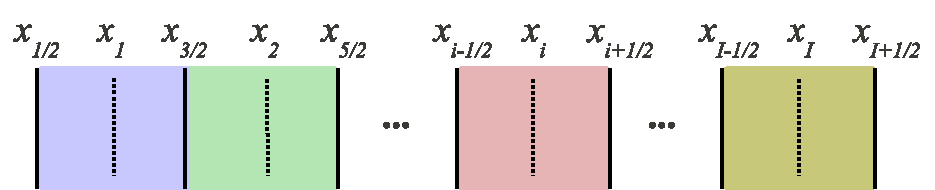
\includegraphics[keepaspectratio, width = 5.0 in]{images/sndisc}
    \caption{Discrete ordinates spatial discretization.}
    \label{fig:sndisc}
\end{figure}

Now, we integrate Eq. \ref{eq:snequation} over cell $i$:
\begin{equation}
  \int^{x_{i+\frac{1}{2}}}_{x_{i-\frac{1}{2}}} dx \Big ( \mu_n \frac{\partial \psi_n}{\partial x} + \Sigma_t(x)\psi_n(x) \Big ) =  \int^{x_{i+\frac{1}{2}}}_{x_{i-\frac{1}{2}}} dx  \Big ( \frac{\Sigma_s(x)}{2} \phi(x) + \frac{S(x)}{2} \Big ) \, ,
\end{equation}
so that
\begin{equation}
   \mu_n ( \psi_{i+\frac{1}{2},n} - \psi_{i-\frac{1}{2},n} ) + \Delta_i \Sigma_{ti}\psi_{i,n} =  \frac{\Delta_i}{2} \Big ( \Sigma_{is} \phi_i +  S_i \Big ) \, ,
\end{equation}
where $\Delta_i \equiv x_{i+\frac{1}{2}} - x_{i-\frac{1}{2}}$ and where the integrals have been approximated via the midpoint rule where needed.  For the sake of brevity, we switch to the emission density, defining
\begin{equation}
 Q_i =  (\Sigma_{is} \phi_i +  S_i)/2 \, ,
\end{equation}
so that
\begin{equation}
   \mu_n ( \psi_{i+\frac{1}{2},n} - \psi_{i-\frac{1}{2},n} ) + \Delta_i \Sigma_{ti}\psi_{i,n} =  \Delta_i Q_i \, .
   \label{eq:discsneq}
\end{equation}

Eq. \ref{eq:discsneq} is a good first step, but we're not done.  Imagine we know the angular flux entering the left side of slab $i$.  We would like to be able to compute the angular flux leaving $i$ to the right.  Doing exactly this over the entire domain is referred to as ``sweeping'' and is a common technique for hyperbolic problems, as it allows us to propagate boundary conditions along the direction of neutron paths.  The problem with Eq. \ref{eq:discsneq} is that we have another unknown: $\psi_{i,n}$, the cell-centered angular flux.  There are several approximations we can use, and we develop two: the diamond difference (DD) and step difference (SD) methods.

For both DD and SD, we define the cell-centered angular flux by
\begin{equation}
 \psi_{i,n} = \frac{1+\alpha_n}{2} \psi_{i+\frac{1}{2},n} + \frac{1-\alpha_n}{2} \psi_{i-\frac{1}{2},n}  \, ,
 \label{eq:ccpsi}
\end{equation}
where
\begin{equation}
 \alpha_n =
 \begin{cases} 0             &   \text{for DD}  \\
               |\mu_n|/\mu_n &   \text{for SD}  \\
 \end{cases} \, .
 \label{eq:alpha}
\end{equation}

The DD method is probably the most ubiquitous of the simple schemes available.  It essentially says the angular flux varies linearly within a cell, and it provides second-order accuracy.  Unfortunately, the DD method can lead to negative fluxes for $\Delta_i$ too large, demonstration of which is left as an exercise.  On the other hand, the SD method cannot yield negative fluxes, but is only first-order accurate.  For the SD method, note that the cell-center angular flux is equal to the incident angular flux at the edge.

\section*{Sweeping Formulas}

We hinted above that we can solve the discrete ordinates equations via use of sweeps across the domain.  In slab geometry, this consists of sweeps to the right for $\mu_n > 0$ and sweeps left for $\mu_n < 0$.  If we have vacuum or some other known boundary flux, we start with that condition, as reflective conditions require information from a sweep having come from the opposite direction.  If all conditions are reflective, a guess must be made for one, which will likely increase the number of iterations required (we'll get to iterations below).

Substituting Eq. \ref{eq:ccpsi} into Eq. \ref{eq:discsneq} and rearranging, we find for sweeping right
\begin{equation}
 \psi_{i+\frac{1}{2},n} = A^+_{i,n} \psi_{i-\frac{1}{2},n} + B^+_{i,n} Q_i \, ,
 \label{eq:rightsweep}
\end{equation}
and sweeping left
\begin{equation}
 \psi_{i-\frac{1}{2},n} = A^-_{i,n} \psi_{i+\frac{1}{2},n} + B^-_{i,n} Q_i \, , 
 \label{eq:leftsweep}
\end{equation}
where
\begin{equation}
 A^{\pm}_{i,n} = \frac{2\mu_n \mp (1 \mp \alpha_m)\Sigma_{ti}\Delta_i}{2\mu_n \pm (1 \pm \alpha_m)\Sigma_{ti}\Delta_i} \, , 
 \label{eq:Aconstant}
\end{equation}
and
\begin{equation}
 B^{\pm}_{i,n} = \frac{\pm 2 \Delta_i}{2\mu_n \pm (1 \pm \alpha_m)\Sigma_{ti}\Delta_i} \, .
 \label{eq:Bconstant}
\end{equation}

\section*{Source Iteration}

When we introduce scattering into the emission density, the right hand side becomes dependent on the solution.  A common way around this is the so-called source iteration method.  The source iteration method is related to the Neumann iteration scheme discussed in Lecture \ref{lec:integral}, and a connection between the two is left as an exercise.  

Source iteration is characterized by a right hand side that lags behind the left hand side.  More explicitly, we solve the equation
\begin{equation}
   \mu_n ( \psi^m_{i+\frac{1}{2},n} - \psi^m_{i-\frac{1}{2},n} ) + \Delta_i \Sigma_{ti}\psi^m_{i,n} =  \Delta_i Q^{m-1}_i \, ,
   \label{eq:discsneqsi}
\end{equation}
where $m$ is the iteration index and 
\begin{equation}
 Q^{m-1} = \frac{1}{2} (\Sigma_{is} \phi^{m-1}_i +  S_i) \, .
\end{equation}
For $m=1$, we need $q^0$.  Often, $\phi^0$ is simply set to zero, unless a better initial guess is easily made.  

The iterations continue until the updated fluxes change insignificantly.  This is usually quantified in a relative sense for the scalar flux by
\begin{equation}
 \frac{ \max | \phi^{m}-\phi^{m-1} |}{\phi^{m-1}}  < \epsilon_{\phi} \, 
 \label{eq:siconvergence}
\end{equation}
for some small $\epsilon_{\phi}$.

\section*{Acceleration}

The discrete ordinates method is in theory a very fast, memory-efficient technique.  Unless the angular flux is needed explicitly, only one set of edge angular fluxes is needed at a time (e.g. the left edge flux for computing the right edge flux, which then can overwrite the left edge flux).  

Despite the algorithmic simplicity of the method, the underlying source iteration scheme can be obnoxiously slow for problems with high scattering ratios.  Several methods have been introduced over the years to accelerate the source convergence.  Of these, diffusion synthetic acceleration (DSA) is probably the most powerful and widespread.  The method essentially involves performing a diffusion solve to update the scalar flux, and has shown spectacular success for a wide variety of problems.  However, DSA can be difficult if not impossible to implement for certain geometries and/or discretization schemes, as it requires a very strict consistency between the transport and diffusion mesh. Instead, we look at two other relatively simple methods that have been quite successful: the \textit{coarse mesh rebalance} (CMR) and \textit{coarse mesh finite difference} (CMFD) methods.

\section*{Coarse Mesh Rebalance}

CMR was probably the first wide-spread method for acceleration discrete ordinates calculations.  Its foundation rests in the \textit{neutron balance equation}, which we obtain in 1-d by integrating Eq. \ref{eq:slabtransportequation} over angle, yielding
\begin{equation}
\begin{split}
 \frac{\partial }{\partial x}J(x) + \Sigma_t(x) \phi(x) = \Sigma_{s}(x)\phi(x) + S(x) \, ,
\end{split}
\label{eq:balance}
\end{equation}
where $J = \mathbf{J}\cdot \hat{i}$ is the net current in the $x$ direction. Now suppose we divide the domain into a number of coarse meshes, indexed by $j$, with cell edges at $x_{j-\frac{1}{2}}$ and $x_{j+\frac{1}{2}}$.  Subtracting the scattering source from both sides and integrating over the $j$th coarse mesh, we obtain
\begin{equation}
\begin{split}
 J_{j+\frac{1}{2}} - J_{j-\frac{1}{2}}  + \int_{x_i} \Sigma_r(x) \phi(x) dx = \int_{x_i} S(x) dx \, .
\end{split}
\end{equation}
Expressing Eq. \ref{eq:net2partial} as $J = J^+ - J^-$, where $+$ indicates to the right and $-$ to the left, we have
\begin{equation}
\begin{split}
 J^+_{j+\frac{1}{2}}- J^-_{j+\frac{1}{2}} - J^+_{j-\frac{1}{2}} + J^-_{j-\frac{1}{2}} + R_j = S_j \, ,
\end{split}
\label{eq:cmrbalance}
\end{equation}
where the partial currents are defined
\begin{equation}
 J^{\pm}_{j+\frac{1}{2}} = \sum_{\mu_n \gtrless 0} \mu_n \psi_{j+\frac{1}{2},n} \, ,
\end{equation}
$R_j$ is the coarse mesh-integrated removal rate, and $S_j$ is the coarse mesh-integrated source.  

Eq. \ref{eq:cmrbalance} must be satisfied by a fully converged fine mesh solution.  For an unconverged iterate, which we denote $\psi^{m+\frac{1}{2}}$, Eq. \ref{eq:cmrbalance} is generally not satisfied.  To force the flux to satisfy neutron balance, we introduce multiplicative rebalance factors $f_j$ such that
\begin{equation}
 \psi^{m+1}_{i,n} =
 \begin{cases} f_j \psi^{m+\frac{1}{2}}_{i,n}     &   x_{j-\frac{1}{2}} < x_{i} < x_{j+\frac{1}{2}} \\
               f_{j-1} \psi^{m+\frac{1}{2}}_{i,n} &   x_{i} = x_{j+\frac{1}{2}} \text{ and } \mu_n > 0 \\
               f_{j+1} \psi^{m+\frac{1}{2}}_{i,n} &   x_{i} = x_{j+\frac{1}{2}} \text{ and } \mu_n < 0 \\
 \end{cases} \, .
 \label{eq:alpha}
\end{equation}
Note the appropriate factor's index denotes from which coarse mesh the neutrons originate. For the case of vacuum boundaries, the corresponding incident partial current vanishes.  For a reflective boundary at the left, $f_0 = f_1$, and similarly for the right boundary.

To illustrate the method, consider a slab with vacuum boundaries divided into three coarse meshes.  Substituting the modified fluxes into the balance equation yields a set of three equations:
\begin{equation}
\begin{split}
  f_1 J^+_{3/2}  - f_2 J^{-}_{3/2}                   + f_1 J^{-}_{1/2} + f_1 R_1 &= f_1 S_1 \\
  f_2 J^+_{5/2}  - f_3 J^{-}_{5/2} - f_1 J^{+}_{3/2} + f_2 J^{-}_{3/2} + f_2 R_2 &= f_2 S_2 \\
  f_3 J^+_{7/2}                    - f_2 J^{+}_{5/2} + f_3 J^{-}_{5/2} + f_3 R_3 &= f_3 S_3 \, ,
\end{split}
\end{equation}
which yields a tridiagonal system written in condensed form as
\begin{equation}
 \mathbf{A} \mathbf{f} = \mathbf{S} \, .
\end{equation}
Solving this equation for $\mathbf{f}$ and updating to $\psi^{m+1}$ allows us to recompute the scattering source, which---hopefully---converges faster than without the rebalancing scheme.  Look to the Further Reading section for references that investigate stability of coarse mesh rebalance.  Algorithm \ref{alg:accel} shows how CMR (or any low order acceleration scheme) can be used within source iteration.

\begin{algorithm}
 \label{alg:accel}
 \caption{Accelerated Source Iteration}
  initialization\;
  \While{$\psi^m$ or $\phi^m$ not converged}{
    compute scattering source \;
    $\psi^{m+\frac{1}{2}} \leftarrow \text{sweep}(\psi^{m})$ \;
    \eIf{using CMR}{
      $\psi^{m+1} \leftarrow \text{cmr}(\psi^{m+\frac{1}{2}})$ \;
    }{
      $\psi^{m+1} \leftarrow \psi^{m+\frac{1}{2}}$ \;
    }
  }
\end{algorithm}



\section*{Coarse Mesh Finite Difference}

The coarse mesh finite difference method has its origins in a nonlinear acceleration technique developed by K. Smith that makes use of discontinuity factors.  With discontinuity factors, any region-integrated high order solution (e.g. from fine mesh transport) can be represented by a low order method (e.g. coarse mesh diffusion).  CMFD makes use of this idea to represent partially converged high order solutions in low order form, followed by subsequent iterations in the low order domain.  This approach is a physical analog of multigrid methods, and its main effect is to dampen low order errors.  What this means is that the high order method will quickly get the ``shape'' right, and a low order acceleration will quickly get the ``magnitude'' right.

We sketch the implementation.  Given a partially converged fine mesh solution, homogenized diffusion coefficients and cross-sections are found for each coarse mesh, as are volume-averaged sources and fluxes.  A coarse mesh diffusion equation is to be solved, but due to an incompletely converged fine mesh solution, discontinuity factors---additive corrections to the effective diffusion coefficients---must be computed to enforce net current continuity between coarse meshes. Once these are defined, the coarse mesh diffusion equations can be solved.  The ratio of the updated average flux to the original average flux of a coarse mesh is used to scale the original fine mesh solution.  The interested student should see the references and exercises for further details.

%  For edge $j+\frac{1}{2}$ joining meshes $j$ and $j+1$, we compute from the high order solution the net current $J_{j+\frac{1}{2}}$ and enforce
% \begin{equation}
%  J_{j+\frac{1}{2}} = -\tilde{D}_{1+\frac{1}{2}} \Big ( \bar{\phi}_{j+1}-\bar{\phi}_{j} \Big ) -\hat{D}_{1+\frac{1}{2}} \Big ( \bar{\phi}_{j+1}-\bar{\phi}_{j} \Big ) \, ,
% \end{equation}
% where
% \begin{equation}
%  \D
% \end{equation}

\section*{A Simple Code}

Here, we provide a simple discrete ordinates code for computing the angular and scalar flux in a slab, given in Listing \ref{list:sn}.  The input requires region (coarse mesh) edge locations, within which the number of fine meshes are defined.  Each region is assigned a material index and volumetric source strength.  The total and scattering cross-sections represent values for different materials; each material can be placed in a region using the appropriate index.  This quick input format allows one to investigate fairly easily a wide range of slab compositions.

Currently, the code is limited to the DD and $S_4$ approximations and vacuum boundaries.  Convergence is tested for $\phi$ only.  The code returns the mesh-centered scalar flux and mesh-edge angular flux.  Within the solver, the notation follows the lecture notation relatively closely.

\lstset{language=Octave,caption=Solution of Slab Problem via Sn, label=list:sn, morecomment=[l]{\%}}
\lstinputlisting{code/sn.m}

% References
\section*{Further Reading}

A good introduction to the discrete ordinates method in 1-d can be found in Chapter 3 in Lewis and Miller \cite{lewis1993cmn}; higher dimensions are covered in Chapter 4 of the same work.  The foundation of the method is usually credited to Chandrasekhar (in the context of stellar radiation) and can be found in his monograph \cite{chandrasekhar1950rt}.  

A review paper by Adams and Larsen \cite{adams2002fim} provides a survey of the many acceleration techniques available for the discrete ordinates equations, and with its several hundred references, is the place to look for further information.  Lewis and Miller provides more information on coarse mesh rebalance, and Cefus and Larsen have assessed its stability \cite{cefus1990sac}.  Park and Cho \cite{park2004cma} have suggested angular-dependent rebalance schemes, and their work is a good place to start to find references to other CMR variations.  The discontinuity factors used in CMFD were first proposed by Smith in the context of homogenization \cite{smith1980shm}, and he later proposed their use for acceleration \cite{smith1983nms}. A recent paper by Zhong et al. \cite{zhong2008itl} provides a modern overview and advanced use of the approach along with a relatively detailed set of equations for implementation.  

Recent advances in the discrete ordinates method include employing advanced Krylov subspace methods, outlined by Warsa, Wareing, and Morel \cite{warsa2004kim}, variations of which are implemented in the state-of-the-art code Denovo \cite{evans2010dnt}.  Moreover, the discrete ordinates equations can be parallelized; the most popular approach is that of Koch, Baker, and Alcouffe \cite{koch1992sfo} (also implemented in Denovo).

For more information on numerical quadrature, see any number of numerical analysis books.  Also, MIT course 18.335 is also highly recommended, as it covers numerical quadrature and many other aspects of numerical methods (including a heavy focus on numerical linear algebra).

\begin{exercises}

  \item \textbf{Negative fluxes}. Using the DD method, express the sweeping step relation in the form
  \begin{equation*}
    \psi_{3/2,n} = A \psi_{1/2,n} + B \, ,
  \end{equation*}
  where $\mu_n > 0$ and $A$ and $B$ are constants to be determined, and eliminate any $\alpha$ terms.  Under what conditions can $\psi_{3/2,n}$ be negative?  Under what conditions, if any, can $\phi_{1,n}$ be negative?  While negative fluxes are not inherently bad numerically, they don't make much physical sense.  Suggest a method for ``fixing'' negative fluxes.

  \item \textbf{Step Difference}.  Implement the step difference method.\footnote{Note, in this and other exercises you are asked to use or modify the given $S_N$ code.  It is also acceptable to use your own code, either written from scratch or via modification of the one given.}

  \item \textbf{Step Characteristic}.  The step characteristic (SC) scheme is another differencing approach based on analytical integration of the transport equation over the fine mesh cell, yielding for example
  \begin{equation*}
    \psi_{i+\frac{1}{2},n}  =  \psi_{i-\frac{1}{2},n} e^{- \frac{\Delta_i \Sigma_{ti}}{\mu}} + \frac{Q_i}{2\Sigma_{ti}} \Big ( 1-e^{-\frac{\Delta_i \Sigma_{ti}}{\mu}} \Big ) \, .
  \end{equation*}
  \begin{enumerate}[(a)]
    \item Derive an expression for $\alpha_{mi}$ as in Eq. \ref{eq:alpha} for use with the SC method.  Note that $\alpha$ in this case is also indexed by the fine mesh index $i$. 
    \item Implement the SC method.
  \end{enumerate}
 
  \item \textbf{Accuracy}.  Here, we want to investigate the accuracy of various difference methods.  To do so, we will use a known analytical solution for as a reference.  See e.g. Appendix A of LeVeque \cite{leveque2007fdm} for more on error analysis.
  \begin{enumerate}[(a)]
    \item Using the $S_6$ approximation, solve \textit{analytically} the discrete ordinates equations for the sample slab problem of Lecture \ref{lec:analytical}.  Implement this reference solution as a function in MATLAB (or your language of choice), so that $\phi(x)$ can be evaluated for any value of $x$.        
    \item Using the DD approximation, solve the $S_6$ equations using 10, 20, 40, 80, and 160, and 320 meshes.  For each case, compute the absolute value of the maximum error between the DD and analytical solution for $\phi$, i.e. find 
    \begin{equation*}
     e^{\text{DD}}_I = \max_{1\leq i \leq I} \Big|\phi^{\text{DD}}_{i}-\phi_{i}^{\text{ref}} \Big |  \, .
    \end{equation*}
    \item Do the same for the SD method.
    \item We say a method is $p$th order accurate if $e(\Delta) \propto \Delta^p$.  Estimate $p$ for both methods. 
    \item Plot the errors for both methods as a function of $\Delta$.  Include also the functions $a\Delta^1$ and $b\Delta^2$, where $a$ and $b$ are constants chosen to yield a nice plot.  Hint: use a log-log plot.
   \end{enumerate}

  \item \textbf{Accuracy: Part Deux}.  Here, we want to investigate the accuracy of the Gauss-Legendre quadrature and hence $S_N$ order.  
  \begin{enumerate}[(a)]
    \item Compute $\phi(x)$ analytically for the sample slab problem of Lecture \ref{lec:analytical}, and make this available as a function.
    \item Compute $\phi$ analytically using the $S_N$ method for orders 2, 4, 8, 16, 32, and 64.  You will have to look up the quadrature parameters for $N > 4$.  
    \item Compute the errors in $\phi$ as in the last problem for $x = 5.0$ and plot as a function of $N$.  
    \item Estimate the ``$p$'' value as in the last problem and comment.  
   \end{enumerate}


  \item \textbf{Reflective Conditions}. Modify the given $S_N$ code to handle reflective conditions, and solve the following problems...

  \item \textbf{CMR}.  Implement CMR in the given $S_N$ code.  Test it on the following problems, using a variety of coarse mesh sizes...

  \item \textbf{CMFD}.  Read the paper by Zhong et al. \cite{zhong2008itl} and derive the CMFD equations in 1-d.  Implement the method in the $S_N$ code and compare it to CMR for the slab configuration given in the last problem.

  \item \textbf{Discrete Ordinates Matrix}.  The discrete ordinates equations are simply a set of coupled differential equations discretized in space and angle.  Consequently, we can express the equations in matrix form.  Consider a uniform slab ($\Sigma_t$ and $\Sigma_s$) with a uniform isotropic source of volumetric strength $S$. Suppose we discretize this slab into three cells of equal width $\Delta$.  Using an $S_2$ approximation with the DD method, and assuming vacuum conditions:
  \begin{enumerate}[(a)]
    \item Cast the sweep-based source iteration scheme in matrix form, expressing the right hand vector in terms of $Q$, the emission density.         
    \item Reformulate the equations so that the source term is brought to the left hand side, thus enabling a direct solution of the equations without source iteration.  
   \end{enumerate}
  For $\Sigma_t = 1.0$, $\Sigma_s = 0.5$, $\Delta = 1.0$, and $S = 1.0$, verify your expressions from parts (a) and (b).  For more on part (b), see the paper by Patton and Holloway \cite{patton2002apg}.

\end{exercises}

\chapter{Nonlinear Acceleration}
\label{lec:nonlinear_acceleration}

The discrete ordinates method is in theory a very fast, memory-efficient 
technique.  Unless the angular flux is needed explicitly, only one set of edge 
angular fluxes is needed at a time (e.g. the left edge flux for computing the 
right edge flux, which then can overwrite the left edge flux).  

Despite the algorithmic simplicity of the method, the underlying source 
iteration scheme can be obnoxiously slow for problems with high scattering 
ratios.  Several methods have been introduced over the years to accelerate the 
source convergence.  Of these, diffusion synthetic acceleration (DSA) is 
probably the most powerful and widespread.  The method essentially involves 
performing a diffusion solve to update the scalar flux, and has shown 
spectacular success for a wide variety of problems.  DSA and related 
methods will be cast as ``preconditioners'' for linear solvers
in the next lecture.

Here, we look at two  relatively simple 
methods that have been quite successful: the \textit{coarse mesh rebalance} 
(CMR) and \textit{Nonlinear Diffusion Acceleration} (NDA) methods.  
Although the presentation is restricted to the one-group case, both 
methods apply readily to multigroup fixed-source and eigenvalue problems.
In addition, both methods can be applied successfully to other 
transport discretization, including the method of characteristics.

\section*{Coarse Mesh Rebalance}

CMR was probably the first wide-spread method for accelerating discrete 
ordinates calculations.  Its foundation rests in the \textit{neutron balance 
equation}, which we obtain in one dimension by integrating
\EQ{eq:slabtransportequation} over angle, leading to
\begin{equation}
\begin{split}
 \frac{\partial }{\partial x}J(x) + \Sigma_t(x) \phi(x) 
   = \Sigma_{s}(x)\phi(x) + S(x) \, ,
\end{split}
\label{eq:balance}
\end{equation}
where $J = \mathbf{J}\cdot \hat{i}$ is the net current in the $x$ direction. Now 
suppose we divide the domain into a number of coarse meshes, indexed by $j$, 
with cell edges at $x_{j-\frac{1}{2}}$ and $x_{j+\frac{1}{2}}$.  Subtracting the 
scattering source from both sides and integrating over the $j$th coarse mesh, we 
obtain
\begin{equation}
\begin{split}
 J_{j+\frac{1}{2}} - J_{j-\frac{1}{2}}  + \int_{x_i} \Sigma_r(x) \phi(x) dx = 
\int_{x_i} S(x) dx \, ,
\end{split}
\label{eq:coarsebalance}
\end{equation}
where $\Sigma_t - \Sigma_s$ is the \textit{removal} cross section.
Expressing \EQ{eq:net2partial} as $J = J^+ - J^-$, where $+$ indicates to 
the right and $-$ to the left, we have
\begin{equation}
\begin{split}
 J^+_{j+\frac{1}{2}}- J^-_{j+\frac{1}{2}} - J^+_{j-\frac{1}{2}} + 
J^-_{j-\frac{1}{2}} + R_j = S_j \, ,
\end{split}
\label{eq:cmrbalance}
\end{equation}
where the partial currents are defined
\begin{equation}
 J^{\pm}_{j+\frac{1}{2}} = \sum_{\mu_n \gtrless 0} \mu_n \psi_{j+\frac{1}{2},n} 
\, ,
\end{equation}
$R_j$ is the coarse mesh-integrated removal rate, and $S_j$ is the coarse 
mesh-integrated source.  

\EQUATION{eq:cmrbalance} must be satisfied by a fully converged fine mesh 
solution.  For an unconverged iterate, which we denote $\psi^{m+\frac{1}{2}}$, 
\EQ{eq:cmrbalance} is generally not satisfied.  To force the flux to 
satisfy neutron balance, we introduce multiplicative rebalance factors $f_j$ 
such that
\begin{equation}
 \psi^{m+1}_{i,n} =
 \begin{cases} f_j \psi^{m+\frac{1}{2}}_{i,n}     &   x_{j-\frac{1}{2}} < x_{i} 
< x_{j+\frac{1}{2}} \\
               f_{j-1} \psi^{m+\frac{1}{2}}_{i,n} &   x_{i} = x_{j+\frac{1}{2}} 
\text{ and } \mu_n > 0 \\
               f_{j+1} \psi^{m+\frac{1}{2}}_{i,n} &   x_{i} = x_{j+\frac{1}{2}} 
\text{ and } \mu_n < 0 \\
 \end{cases} \, .
 \label{eq:alpha}
\end{equation}
Note the appropriate factor's index denotes from which coarse mesh the neutrons 
originate. For the case of vacuum boundaries, the corresponding incident partial 
current vanishes.  For a reflective boundary at the left, $f_0 = f_1$, and 
similarly for the right boundary.

To illustrate the method, consider a slab with vacuum boundaries divided into 
three coarse meshes.  Substituting the modified fluxes into the balance equation 
yields a set of three equations:
\begin{equation}
\begin{split}
  f_1 J^+_{3/2}  - f_2 J^{-}_{3/2}                   + f_1 J^{-}_{1/2} + f_1 R_1 
&= f_1 S_1 \\
  f_2 J^+_{5/2}  - f_3 J^{-}_{5/2} - f_1 J^{+}_{3/2} + f_2 J^{-}_{3/2} + f_2 R_2 
&= f_2 S_2 \\
  f_3 J^+_{7/2}                    - f_2 J^{+}_{5/2} + f_3 J^{-}_{5/2} + f_3 R_3 
&= f_3 S_3 \, ,
\end{split}
\end{equation}
which yields a tridiagonal system written in condensed form as
\begin{equation}
 \mathbf{A} \mathbf{f} = \mathbf{S} \, .
\end{equation}
Solving this equation for $\mathbf{f}$ and updating to $\psi^{m+1}$ allows us to 
recompute the scattering source, which---hopefully---converges faster than 
without the rebalancing scheme.  Look to the Further Reading section for 
references that investigate stability of coarse mesh rebalance.  
Algorithm~\ref{alg:accel} shows how CMR (or any low order acceleration scheme) 
can be used within source iteration.

\begin{algorithm}
 \label{alg:accel}
 \caption{Accelerated Source Iteration}
  initialization\;
  \While{$\psi^m$ or $\phi^m$ not converged}{
    compute scattering source \;
    $\psi^{m+\frac{1}{2}} \leftarrow \text{sweep}(\psi^{m})$ \;
    \eIf{using CMR}{
      $\psi^{m+1} \leftarrow \text{cmr}(\psi^{m+\frac{1}{2}})$ \;
    }{
      $\psi^{m+1} \leftarrow \psi^{m+\frac{1}{2}}$ \;
    }
  }
\end{algorithm}



\section*{Nonlinear Diffusion Acceleration}

Nonlinear Diffusion (or Coarse-Mesh, Finite-Difference) Acceleration (NDA
or CMFD) was originally developed by Kord Smith as a way to reduce the 
memory requirements of advanced, nodal-diffusion solvers \cite{smith1983nms}.  
The method also
led to signficant speed-ups and has since been applied routinely in 
for lattice-physics computations based on the method of characteristics
\cite{2002}.  

We begin along the same lines as we did for CMR by integrating the 
transport equation over a coarse mesh indexed by $j$, which leads to 
\EQ{eq:coarsebalance}.  Now, define the flux-weighted cross section
\begin{equation}
 \Sigma_{t,j} = \frac{\int^{x_{j+1/2}}_{x_{j-1/2}} \Sigma_r(x) \phi^{n+1/2} dx}
                     {\int^{x_{j+1/2}}_{x_{j-1/2}}\phi^{n+1/2} dx} \, ,
\end{equation}
with similar expressions for $\Sigma_{r,j}$ and $\Sigma_{s,j}$, along 
with the coarse-mesh-averaged flux
\begin{equation}
 \phi_{j} = \frac{\int^{x_{j+1/2}}_{x_{j-1/2}} \phi(x) dx}
              {\int^{x_{j+1/2}}_{x_{j-1/2}} dx} \, 
\end{equation}
and source
\begin{equation}
 S_{j} = \frac{\int^{x_{j+1/2}}_{x_{j-1/2}} S(x) dx}
              {\int^{x_{j+1/2}}_{x_{j-1/2}} dx} \, .
\end{equation} 
With these definitions, \EQ{eq:coarsebalance} can be written as
\begin{equation}
 J^{n+1/2}_{j+1/2} - J^{n+1/2}_{j-1/2} 
   + \Delta_j \Sigma_{r,j} \phi_j = \Delta_j S_j
\end{equation}

Previously, we studied fine-mesh diffusion, which gave
\begin{equation}
\begin{split}
  J^{n+1/2}_{j+1/2} &= - \left ( \frac{ 2 D_j D_{j+1} }
                                     {D_j \Delta_{j+1} + D_{j+1} \Delta_j}
                        \right )
                        (\phi_{j+1} - \phi_j) \\\
                    &= \tilde{D}_{j+1/2} (\phi_{j+1} - \phi_j) \, .
\end{split}                    
\label{eq:diffusion_current}
\end{equation}
where $D_j$ is the diffusion coefficient for the $j$th coarse cell.
Although the choice of $D_j$ is not unique, a common approach is 
to set 
\begin{equation}
 D_j = 1/3\Sigma_{t, j}
\end{equation}
or 
\begin{equation}
 D_{j} = \frac{\int^{x_{j+1/2}}_{x_{j-1/2}} D(x) \phi(x) dx}
              {\int^{x_{j+1/2}}_{x_{j-1/2}} \phi(x) dx} \, .
\end{equation}
A better approach may be to weight $D(x)$ by $J(x)$ instead of 
$\phi(x)$, but in practice $J(x)$ is not usually computed.

Even with a flux- or current-weighted $D_j$, the current as 
defined by \EQ{eq:diffusion_current} is not generally 
equal to the current as computed directly from 
$\psi^{n+1/2}$, as in Eq. XXX, because the diffusion approximation is 
not guaranteed to yield the same solution as a transport 
approximation.  Hence, even if the flux were perfectly converged, 
the diffusion approximation, coarse mesh or otherwise, will not 
reproduce the solution and, hence, does not preserve balance over
the coarse cells.

We can enforce balance by letting
\begin{equation}
 J_{j+1/2} = -\tilde{D}_{j+1/2} (\phi_{j+1}-\phi_j) - \hat{D}_{j+1/2}(\phi_{j+1}+\phi_j) \, ,
\end{equation}
where the nonlinear coupling coefficient $\hat{D}_{j+1/2}$ is 
defined as
\begin{equation}
 \hat{D}_{j+1/2} = \frac{\tilde{D}_{j+1/2} (\phi_{j+1}-\phi_j) + J_{j+1/2}}{\phi_{j+1}+\phi_j)} \, .
\end{equation}
For an albedo condition at the left, we can set 
\begin{equation}
 J_{1/2} = (\tilde{D}_{1/2}+\hat{D}_{1/2})\phi_1 \, ,
\end{equation}
where 
\begin{equation}
 \hat{D}_{1/2} = \frac{J_{1/2}-\tilde{D}_{1/2} \phi_1}{\phi_1} \, .
\end{equation}
The resulting, one-dimensional diffusion equation is
\begin{equation}
\begin{split}
 -\tilde{D}_{j+1/2}(\phi_{j+1}-\phi_j) - \hat{D}_{j+1/2} & (\phi_{j+1}+\phi_j)  + \\
 \tilde{D}_{j-1/2}(\phi_{j}-\phi_{j-1})& + \hat{D}_{j-1/2} (\phi_{j}+\phi_{j-1}) + \\
  & \Sigma_{r,j} \phi_{j}^{n+1} \Delta_j = S_j \Delta_j \, .
\end{split}
\end{equation}



Once solved, the coarse-mesh flux $\phi^n$ can be used to 
update the fine-mesh flux via 
\begin{equation}
 \phi^{n+1}(x) = \frac{\phi^{n}_{j}}{\phi^{n-1/2}_j} \phi(x) \, \quad x \in [x_{j-1/2},x_{j+1/2}] \, .
\end{equation}
With $\phi^{n}(x)$ found, the scattering source can be updated,  another 
sweep can be performed to obtain $\psi^{n+3/2}$, and the
process can be repeated. 


Like CMR, if the NDA converges, it must converge to 
the right answer.  However, that convergence is not guaranteed \cite{}.
Sometimes, for a given $\tilde{D}$, the computed $\hat{D}$ leads to 
a diffusion matrix that is not diagonally dominant.  While this does 
not prevent solution of the equations, the updated, coarse-mesh flux 
may contain unphysical features that lead to instability.  
Specifically, if $\hat{D}_{j+1/2} > \tilde{D}_{j+1/2}$, setting
\begin{equation}
 \hat{D}_{j+1/2} = \tilde{D}_{j+1/2} = \frac{J_{j+1/2}}{2\phi_j} \, 
\end{equation}
ensures a diagonally-dominant matrix.

In addition, the use of $D_j$ directly may be replaced by 
Larsen's ``effective'' diffusion coefficient, which may be particularly
valuable for the step-characteristic scheme in use for both MOC and S$_N$
calculations.  Even though $D_j$ is arbitary, its proper selection can 
help convergence.


Finally, it has been found that instabilities can be reduced 
significantly by using under-relaxation of the 
nonlinear coupling coefficient \cite{}.  In other words, 
the coefficients are defined
\begin{equation}
 \hat{D}^{n+1}_{j+1/2} = \alpha \hat{D}^{n+1}_{j+1/2} + (1-\alpha)\hat{D}^{n}_{j+1/2}  \, ,
\end{equation}
where  $\alpha \in [0, 1)$ is the relaxation parameter.  Based on 
past experience, typical values for $\alpha$ range from 0.5 to 0.8, 
though the optimum value is highly problem dependent.





\section*{Further Reading}

A review paper by Adams and Larsen \cite{adams2002fim} provides a survey of the 
many acceleration techniques available for the discrete ordinates equations, and 
with its several hundred references, is the place to look for further 
information.  Lewis and Miller provides more information on coarse mesh 
rebalance, and Cefus and Larsen have assessed its stability \cite{cefus1990sac}. 
 Park and Cho \cite{park2004cma} have suggested angular-dependent rebalance 
schemes, and their work is a good place to start to find references to other CMR 
variations.  The discontinuity factors used in CMFD were first proposed by Smith 
in the context of homogenization \cite{smith1980shm}, and he later proposed 
their use for acceleration \cite{smith1983nms}. A recent paper by Zhong et al. 
\cite{zhong2008itl} provides a modern overview and advanced use of the approach 
along with a relatively detailed set of equations for implementation.  


%  For edge $j+\frac{1}{2}$ joining meshes $j$ and $j+1$, we compute from the high order solution the net current $J_{j+\frac{1}{2}}$ and enforce
% \begin{equation}
%  J_{j+\frac{1}{2}} = -\tilde{D}_{1+\frac{1}{2}} \Big ( \bar{\phi}_{j+1}-\bar{\phi}_{j} \Big ) -\hat{D}_{1+\frac{1}{2}} \Big ( \bar{\phi}_{j+1}-\bar{\phi}_{j} \Big ) \, ,
% \end{equation}
% where
% \begin{equation}
%  \D
% \end{equation}

\chapter{Iterative Solvers for Transport Equations}
\label{lec:iterative_solvers}

So far, three basic models for discretizing the transport equations have been
discussed.  The latter model, neutron diffusion, leads to a very 
straightforward system of linear equations for which standard techniques
readily apply.  The S$_{\text{N}}$ and MOC transport schemes also lead 
to a set of linear equations.  However, casting these equations in a 
standard form for solution by generic solvers is less obvious.   Because
our goal is ultimately to apply generic solvers to the equations, it
is useful here first to provide a general representation of the equations.

\subsection{Angular Flux Equations}

Before proceeding, we adopt an operator notation following Larsen 
and Morel \cite{larsen2010ado} to simplify
somewhat the exposition to follow.  
Recall that the scalar flux is defined
\begin{equation}
\begin{split}
  \phi(\vec{r}) &= \int_{4\pi} d \Omega \, 
                   \psi(\vec{r}, \Omega) \\
              &\approx \sum_{n = 1}^N w_n \psi_{n}(\vec{r}) \, .
\end{split}
\end{equation}
Introducing a \emph{discrete-to-moment} operator $\oper{D}$, we
enforce
\begin{equation}
 \phi = \oper{D} \psi \, ,
\end{equation}
where space and angle indices are implicit.  Moreover, we introduce
a \emph{moment-to-discrete} operator $\oper{M}$, defined
\begin{equation}
 \psi = \oper{M} \phi \, ,
\end{equation}
where in general
$\oper{D} \ne \oper{M}^{-1}$.  Finally,
defining the operator
\begin{equation}
 \oper{L} (\cdot) \equiv 
 \left ( \hat{\Omega} \cdot \nabla + 
   \Sigma_{t}(\vec{r}) \right ) (\cdot) \, ,
\end{equation}
the one group discretized transport equation becomes
\begin{equation}
  \oper{L}\psi = \oper{M}\oper{S}\phi + q \, ,
\label{eq:wgteop_psi}
\end{equation}
where $\oper{S}$ is the scattering operator (which can include
fission).  For the case of
isotropic scattering in one group, we have
$\oper{M} = \frac{1}{4\pi}$
while $\oper{S} = \Sigma_s(\vec{r})$.

For the multigroup problem, this notation generalizes to 
\begin{equation}
  \oper{L}_g\psi_g =  \oper{M} \sum_{g'=1}^G 
         \left (
           \oper{S}_{gg'} + 
           \frac{1}{k}\oper{X}_{g} \oper{F}_{g'} 
         \right )\phi_{g'} + q_g \, ,
\label{eq:mgteop_psi}
\end{equation}
where the fission source has been explicitly represented.  Here,
$\oper{X}$ represents the fission spectrum $\chi$ in operator form.

\subsection{Moments Equation}

\subsubsection{S$_{\text{N}}$ in Operator Form}

Equations \ref{eq:wgteop_psi} and \ref{eq:mgteop_psi} represent 
equations in which the unknown is the angular flux $\psi$.  In 
general, and particularly for reactor physics, our interest is in
computing reaction rates for which only the scalar flux is needed.  
Consequently, in practice the angular flux is rarely stored explicitly, 
but is rather computed on-the-fly during a sweep through the space-angle 
grid.  This
can be represented explicitly by manipulating the equations to be functions
only of the scalar flux (and higher order flux moments if scattering 
is anisotropic).  

To illustrate, consider Eq. \ref{eq:wgteop_psi}.  Multiplying
through by the space-angle \emph{transport sweep} 
operator $\oper{T} = \oper{DL}^{-1}$, we have
\begin{equation}
 \oper{D}\psi = 
    \oper{DL}^{-1} \oper{MS} \phi + \oper{DL}^{-1}q \, .
\end{equation}
Recalling $\phi = \oper{D}\psi$ and rearranging yields 
\begin{equation}
 (\oper{I} - \oper{TMS} ) \phi =  \oper{T}q \, ,
\label{eq:wgteop}
\end{equation}
or 
\begin{equation}
  \oper{A}_{\text{WG}} \phi = b \, ,
\end{equation}
where
\begin{equation}
 \oper{A}_{\text{WG}} \equiv \oper{I} - \oper{TMS}
\end{equation}
is the \emph{within-group transport operator} and
\begin{equation}
 b = \oper{T}q
\end{equation}
represents the \emph{uncollided} flux moments.  Eq. \ref{eq:wgteop} represents
a linear equation in standard form for the scalar flux moments $\phi$.  

The operator $\oper{DL}^{-1}$ has 
a very specific physical interpretation.  The inverse $\oper{L}^{-1}$
represents the set of space-angle sweeps from one global boundary 
to another.  The additional factor  $\oper{D}$ implies that along
the space-angle sweep, $\phi$ is updated, thus eliminating the 
need to store $\psi$.  This is exactly how S$_{\text{N}}$ and MOC solvers 
have traditionally been implemented.  

The extension to multigroup yields a similar form
\begin{equation}
   \left ( \oper{I} - \oper{T_{\text{MG}}M_{\text{MG}}} 
      \left ( \oper{S}_{\text{MG}} + 
              \frac{1}{k}\oper{X}_{\text{MG}} \oper{F}_{\text{MG}}^{\transp} 
      \right ) 
   \right ) \phi 
   =  \oper{T_{\text{MG}}}q_{\text{MG}} \, ,
\label{eq:mgteop}
\end{equation}
where $\oper{T_{\text{MG}}}$  and $\oper{M_{\text{MG}}}$ are  block 
diagonal operators
having blocks 
$\oper{T}_g$ and $\oper{M}$, 
respectively, 
$\oper{X_{\text{MG}}}$, $\oper{F_{\text{MG}}}$, and $q_{\text{MG}}$ 
are the 
column vectors having elements 
$\oper{X}_g$, $\oper{F}_g$, and $q_g$
respectively, and the multigroup scattering operator is defined
\begin{equation}
       \oper{S_{\text{MG}}} = 
           \left(
           \begin{array}{ccc}
              \oper{S}_{11} & \cdots & \oper{S}_{1G} \\
              \vdots           & \ddots & \vdots          \\
              \oper{S}_{G1} & \cdot   & \oper{S}_{GG}
           \end{array} 
           \right ) \, .
\label{eq:mgscatter}
\end{equation}
Similar to the within-group problem, we define the \emph{multigroup
transport operator} to be
\begin{equation}
 \oper{A}_{\text{MG}} =  \oper{I} - \oper{T_{\text{MG}}M_{\text{MG}}} 
      \left ( \oper{S}_{\text{MG}} + 
              \frac{1}{k}\oper{X}_{\text{MG}} \oper{F}_{\text{MG}}^{\transp} 
      \right ) \, .
 \label{eq:mgto}
\end{equation}

\subsubsection{MOC in Operator Form}

While the operators and equations apply directly the S$_{\text{N}}$ method,
slight changes must be made to represent MOC. In MOC, we iterate on the 
quantities averaged over a \emph{cell},
specifically the scalar flux moments $\phi_{\text{cell}}$.  However, the
angular fluxes are computed for each track \emph{segment}, and each cell 
can have several tracks crossing it.  The average angular flux on each 
track segment in a given cell is used to generate the average scalar flux.

This can be cast in operator form for a one group problem as
\begin{equation}
  \oper{L}\psi_{\text{seg}} = 
    \oper{P M S}\phi_{\text{cell}} +
      \oper{P} q_{\text{cell}} \, ,
    \label{eq:traneq}
\end{equation}
where $q_{\mathrm{cell}}$ is the cell-wise external source
and $\oper{P}$ is a cell-to-segment operator, ``P'' denoting prolongation,
though not quite in the multigrid sense.  

We can also define a segment-to-cell operator (restriction) 
$\oper{R}$ so that
\begin{equation}
   \psi_{\text{cell}} = \oper{R}\psi_{\text{seg}} \, ,
\end{equation}
and
\begin{equation}
    \phi_{\text{cell}} = \oper{DR}\psi_{\text{seg}} \, . 
    \label{eq:psitophi}
\end{equation}
Finally, the moments equation akin to Eq. \ref{eq:wgteop} is
\begin{equation}
   \left ( \oper{I} -  \oper{DRL}^{-1}\oper{PMS} \right ) 
     \phi_{\text{cell}} =  
  \oper{DRL}^{-1}\oper{P} q_{\text{cell}}  \, .
\end{equation}
In the context of MOC, the operator
\begin{equation}
 \oper{A}_{\text{WG-MOC}} =  \oper{I} -  \oper{DRL}^{-1}\oper{PMS} 
\end{equation}
is implied when discussing the within-group transport operator, and 
similarly for the multigroup variant.

\subsection{Boundary Conditions}

So far, we have neglected to treat boundary conditions.  
In particular, reflecting (or periodic, or white) boundary conditions 
create an additional set of unknowns, namely the incident 
(or exiting) boundary fluxes.  In theory, treating these conditions is
straightforward, but we refrain from further discussion for two 
reasons. First, adding boundary unknowns complicates presentation of 
the algorithms discussed below.  Second, and more importantly,
response function calculations use vacuum conditions 
only, and so treatment of reflecting boundaries is outside our scope.
A more detailed discussion can be found in the work 
of Warsa \emph{et al.} \cite{warsa2004kim}.

\section{Transport Solvers}

Consider the fixed source multigroup transport problem
represented by
\begin{equation}
 \oper{A}_{\text{MG}} \phi = b \, .
\end{equation}
The traditional method for solving the multigroup equations is via 
a nested iteration in which a series of within-group equations is 
solved for each group, with the scattering (and possibly) fission 
sources updated between each group solve.  More modern treatments
view the equations as a complete set to be solved simultaneously.


\subsection{Gauss-Seidel}

The Gauss-Seidel method has long been used to solve the multigroup 
equations.  For standard problems, the method first solves the 
fast (within-)group equation.  The updated fast group flux can then be used 
to define the in-scatter source for the next group, and so on.  Because
this algorithm really implies inversion of each group \emph{block} (as 
defined in Eq. \ref{eq:mgteop}), the method is more accurately described 
as \emph{block} Gauss-Seidel in energy.


Algorithm \ref{alg:gauss_seidel_energy} describes a basic implementation 
of the method.  Historically, convergence of the method is based on the 
difference of successive fluxes, either as an absolute norm as indicated 
or a norm of the relative point-wise difference.  Assessing convergence 
in this way can be misleading.  The difference between successive
iterates can be much smaller than the difference between an iterate
and the solution, sometimes resulting in premature convergence.  Section 
\ref{sec:comparison_of_norms} provides a numerical comparison of various
convergence criteria.

\begin{algorithm}[h]
  \SetCommentSty{small}
  \DontPrintSemicolon
  \KwData{initial guess for group fluxes $\phi^{(0)}$, 
          external source $q$, 
          eigenvalue $k$, 
          tolerance $\tau$,
          maximum number of iterations $N$}
  \KwResult{converged group fluxes $\phi$}
  $n = 1$ \;
  \While{$\tau > \epsilon$ and $n < N$}
  {
    \For{$g$ from 1 to $G$}
    {
      \tcp{Compute in-scatter and in-fission sources}
      $b_g = \oper{T}_g \left(  \oper{M} \sum_{g'=1}^G 
              \left ( \oper{S}_{gg'} + \frac{1}{k}\oper{X}_{g} \oper{F}_{g'} 
              \right )\phi^{(n-1)}_{g'} + q_g \right )$ \;
      \tcp{Solve the within-group problem}
      $\phi^{(n)}_{g} = \oper{A}^{-1}_g b_g$ \;
    }
    $\tau = ||\phi^{(n)}-\phi^{(n-1)}||$\;
    $n = n + 1$\;
    
  }
  \caption{Gauss-Seidel Algorithm for the Multigroup Transport Equation}
  \label{alg:gauss_seidel_energy}
\end{algorithm}

For problems in which there is no upscatter and no fission, Gauss-Seidel
is an essentially exact scheme assuming the within-group equations are
solved exactly.  However, for cases with upscatter or fission, 
extra ``upscatter'' iterations are required, and in some cases, 
the convergence of Gauss-Seidel becomes prohibitively slow.

\subsection{Source Iteration}
\index{source iteration}
\index{Richardson iteration|see{source iteration}}
The standard method for solving the within-group transport equation
has been \emph{source iteration}. The basic idea is a simple one:
given an external source (including in-scatter and fission), we guess the 
flux, compute the within-group scattering source, solve for a new flux, and 
repeat until converged.  Mathematically, source iteration is 
defined by the process 
\begin{equation}
 \phi^{(n)} = \oper{TMS}\phi^{(n-1)} + \oper{T}q \, .
\end{equation}
However, recall that Richardson iteration for the system $\oper{A}x=b$ 
is just 
\begin{equation}
 x^{(n)} = (\oper{I}-\oper{A})x^{(n-1)} + b \, .
\end{equation}
Since $\oper{I} - \oper{A}_{\text{WG}} = \oper{TMS}$, we see that 
source iteration is equivalent to Richardson iteration.

Source iteration has a particularly intuitive physical interpretation.
Suppose our initial guess is zero.  The resulting flux is just the 
right hand side, or the uncollided flux.  Performing one iteration 
adds the contribution of neutrons having undergone a single collision.
A second iteration includes the twice-collided neutrons, and so on. 
For systems in which neutrons undergo many scattering events, the physics 
suggests the process can be painfully slow to converge.  The math verifies
the physics \cite{larsen2010ado}: the error $||\phi^{(n)}-\phi^{(n-1)}||$ of 
the infinite medium one group problem goes as the scattering 
ratio $c = \frac{\Sigma_s}{\Sigma_t}$, meaning that increased scattering
leads to slower convergence.

\subsection{Krylov Solvers}
\label{sec:krylovsolvers}

Because of the limitations of the Gauss-Seidel and source iteration
schemes, much work has been done to apply modern linear solvers to
transport problems.  One of the most successful class of solvers 
studied consists of Krylov subspace methods.  

\subsubsection{Overview}

One can categorize linear (and eigenvalue) solvers as being 
\emph{stationary} or \emph{nonstationary}.  Stationary methods
produce updated solutions using only a single previous solution, and
the Gauss-Seidel and Richardson methods are both stationary.  Other 
well-known examples include the Jacobi and 
successive over-relaxation (SOR) methods.
On the other hand, nonstationary methods produce a solution based on 
two or more previous iterates (or the information used to create those 
iterates). 

Krylov methods are nonstationary methods that rely on 
construction of a so-called \emph{Krylov subspace} of dimension $n$, 
defined for an $m \times m$ operator $\oper{A}$ as
\begin{equation}
 \mathcal{K}(n,x_0) \equiv \text{span} 
     \{x_0,\, \oper{A}x_0,\, \oper{A}^2x_0,\, 
         ,\ldots,\,, \oper{A}^{m-1}x_0 \} \, , 
 \label{eq:krylovsubspace}
\end{equation}
for some initial, possibly random, vector $x_0$.  The main idea of Krylov
subspace methods is to find  $x \in \mathcal{K}(m,x_0)$  
 that ``best'' solves the system of interest, be it an 
eigenproblem or linear system, where it is assumed that $m \ll n$.

Working with $\mathcal{K}(n, x_0)$ directly is difficult numerically, since
repeated application of $\oper{A}$ sends the initial vector $x_0$ into the
same direction, namely that of the dominant eigenvector of $\oper{A}$.  
Hence, the basis 
must be orthogonalized. The canonical approach for nonsymmetric 
operators is Arnoldi's method, which by successive application of the 
modified Gram-Schmidt process yields the Arnoldi decomposition
\begin{equation}
 \oper{A}\oper{V} = \oper{V} \oper{H} + fe^{\transp}_m \, ,
\end{equation}
where $\mathbf{V} \in \mathbb{R}^{m\times n}$  consists of
orthonormal columns,
$\mathbf{H} \in \mathbb{R}^{n \times n} $ is an upper Hessenberg matrix, 
$e_n$ is the
$n$-vector of all zeros except a one in the $n$th location, and $f$ is 
the residual, which is orthogonal to the columns of $\mathbf{V}$.  

The most popular Krylov method for nonsymmetric linear systems (such as the 
transport equations above) is GMRES \cite{saad1986gmr}.  The basic idea 
of GMRES is straightforward:  the $n$th step of GMRES produces a 
$n\times n$ Hessenberg matrix and the corresponding basis $\oper{V}$,
and the approximate solution $x_n$ is found by minimizing the residual 
norm $||r||_2 = ||\oper{A}x_n-b||_2$
for $x_i \in \mathcal{K}(n, x_0)$.  In other words, $x_n$ must be in 
the column space of $\mathcal{K}(n, x_0)$, mathematically 
expressed as $x_n = \oper{V} y$,  where 
$y$ satisfies 
\begin{equation}
\begin{split}
  ||\oper{AV}y-b||_2 &= ||\oper{V}^{\transp} \oper{A} \oper{V} x_n -\oper{V}^{\transp} b|| \\
                     &= || \oper{H} y - \oper{V}^{\transp} b || \, .
\end{split}
\end{equation}
The last equation shows that GMRES can be thought of as finding the 
best solution $x_n \in \mathcal{K}(n, x_0)$ in a least-squares sense.

\subsubsection{Preconditioning}

While Krylov methods are generally more robust than the classical 
stationary methods, their performance can be improved significantly
via \emph{preconditioning}.  A preconditioner $\oper{M}$ is an operator 
whose inverse satisfies $\oper{M}^{-1} \approx \oper{A}^{-1}$ in some sense 
and is relatively inexpensive to apply.

A \emph{left preconditioned} linear system is
\begin{equation}
  \oper{M}^{-1}\oper{A}x = \oper{M}^{-1}b
\end{equation}
while a \emph{right preconditioned} system is 
\begin{equation}
  \oper{A}\oper{M}^{-1} y = b
\end{equation}
with $x = \oper{M}^{-1} y$.  The left preconditioned residual differs 
from the original residual but may be a better metric for convergence. 
The right preconditioned system preserves the original residual.  

A preconditioner typically leads to a clustering of eigenvalues.  As 
an extreme example, suppose that $\oper{M} = \oper{A}$.  The 
preconditioned operator is then $\oper{AM}^{-1} = \oper{I}$, for 
which all the eigenvalues are unity.  Of course, to apply $\oper{M}^{-1}$ 
in this case represents solving the original problem.  While preconditioners
cannot in general be expected to yield a set of eigenvalues equal to unity, 
any clustering typically improves convergence.  Often, even pushing 
eigenvalues away from the origin tends to improve 
convergence \cite{larsen2010ado}.
Chapter \ref{chp:transport_pc} provides a relatively thorough 
development of several diffusion-based preconditioners for the 
transport equation.

\subsubsection{Krylov Methods for the Transport Problems}

Krylov solvers have been used 
to solve both the within-group \cite{warsa2004kim} and multigroup
\cite{evans2010tdf} transport equations.  For the multigroup 
equations in particular, the independent nature of the group-wise 
blocks makes parallelization in energy much more straightforward
than for Gauss-Seidel.

For problems in which there is no fission and 
upscatter is limited to a subset of thermal groups, it is
possible to solve the downscatter groups via Gauss-Seidel
and to use a Krylov method on the thermal block of Eq. \ref{eq:mgteop}.
Doing so can yield improved efficiency for some problems \cite{evans2010tdf}.  
However, when fission is included, as is often true for response 
function generation, there is always
thermal-to-fast coupling, and solving the full system via
a Krylov method is to be preferred.


\chapter{Linear Acceleration}
\label{lec:linear_acceleration}


While Krylov methods are generally more robust than the classical 
stationary methods, their performance can be improved significantly
via \emph{ preconditioning}.  A preconditioner $\oper{M}$ is an operator 
whose inverse satisfies $\oper{M}^{-1} \approx \oper{A}^{-1}$ in some sense 
and is relatively inexpensive to apply.

A \emph{ left preconditioned} linear system is
\begin{equation}
  \oper{M}^{-1}\oper{A}x = \oper{M}^{-1}b
\end{equation}
while a \emph{ right preconditioned} system is 
\begin{equation}
  \oper{A}\oper{M}^{-1} y = b
\end{equation}
with $x = \oper{M}^{-1} y$.  The left preconditioned residual differs 
from the original residual but may be a better metric for convergence. 
The right preconditioned system preserves the original residual.  

A preconditioner typically leads to a clustering of eigenvalues.  As 
an extreme example, suppose that $\oper{M} = \oper{A}$.  The 
preconditioned operator is then $\oper{AM}^{-1} = \oper{I}$, for 
which all the eigenvalues are unity.  Of course, to apply $\oper{M}^{-1}$ 
in this case represents solving the original problem.  While preconditioners
cannot in general be expected to yield a set of eigenvalues equal to unity, 
any clustering typically improves convergence.  Often, even pushing 
eigenvalues away from the origin tends to improve 
convergence \cite{larsen2010ado}.
Chapter \ref{chp:transport_pc} provides a relatively thorough 
development of several diffusion-based preconditioners for the 
transport equation.



Chapter \ref{chp:transport_methods} provided a short survey of trends in 
transport discretizations and solvers applicable to the fixed source 
multiplying problems relevant to response matrix methods.  As noted, 
Krylov methods have quickly become important tools for a variety of 
transport problems, but to be successful, they require adequate 
\emph{ preconditioning}.  
This chapter details several preconditioners 
relevant to transport calculations for reactor physics, and specifically 
the comparatively small problems characteristics of response matrix 
methods.

\index{preconditioner}

\section{Diffusion Synthetic Acceleration}
\index{DSA|see{diffusion synthetic acceleration}}
\index{diffusion synthetic acceleration}

Frequently, the most successful preconditioners are those that are based 
on \emph{ a priori} knowledge of the physics or structure of the problem.
This has long been the case for accelerating transport problems, for 
which early techniques enforced balance over coarse regions in space, 
angle, and energy.  

A related idea that has remained an important 
innovation is to apply a simple, low order approximation, invariably
based on diffusion, to provide an efficient update or correction to 
an unconverged transport solution.  Here, we provide a brief sketch 
of one diffusion-based scheme known as \emph{ diffusion synthetic 
acceleration} that has long been used but only recently as a 
preconditioner.  For simplicity, the development is given for the 
one group case, following the excellent treatment 
of Larsen and Morel \cite{larsen2010ado}.

Suppose we perform one source iteration, so that
\begin{equation}
  \phi^{n+\frac{1}{2}} = \oper{TMS} \phi^{n} + \oper{T}q \, .
\end{equation}
where $\oper{S}$ is assumed to contain both the 
scatter and fission within-group terms.
 Note the half index.  We subtract this equation 
from Eq. \ref{eq:wgteop} to get
\begin{equation}
 (\oper{I} - \oper{T}\oper{MS})\phi- \phi^{n+\frac{1}{2}} = 
   -\oper{TMS} \phi^{n} \, ,
\end{equation}
and adding $\oper{TMS} \phi^{n+\frac{1}{2}}$ to both 
sides and rearranging, 
\begin{equation}
 \epsilon = \overbrace{ ( \oper{I} - \oper{TMS})^{-1}\oper{T M} }^
                      {\text{what we approximate}}
            \overbrace{\oper{S} (\phi^{n+\frac{1}{2}}- \phi^{n})}^{v}
\label{eq:erroreq}
\end{equation}
where $\epsilon$ is the error.  Note the error satisfies the 
transport equation
\begin{equation}
 (\hat{\Omega} \cdot \nabla  + \Sigma) \varepsilon - 
   \frac{\Sigma_s}{4\pi} \epsilon =  \frac{v}{4\pi} \, ,
\end{equation}
where
\begin{equation}
 \epsilon = \int_{4\pi} d\Omega \, \varepsilon \, .
\end{equation}
Solving the error equation is just as expensive as solving the 
original transport equation.  As an alternative, we can use the 
diffusion approximation.  In this case, we have
\begin{equation}
 (-\nabla \cdot D \nabla + \Sigma - \Sigma_s) \epsilon = v \, ,
\end{equation}
or in operator form,
\begin{equation}
  \epsilon = \oper{C}^{-1} v = 
    \oper{C}^{-1} \oper{S} (\phi^{n+\frac{1}{2}}- \phi^{n}) \, .
\end{equation}
This leads to the update
\begin{equation}
\begin{split}
 \phi \approx \phi^{n+1} 
   &= \phi^{n+\frac{1}{2}} + 
      \oper{C}^{-1} \oper{S} (\phi^{n+\frac{1}{2}}- \phi^{n}) \\
   &= (\oper{I} + \oper{C}^{-1} \oper{S}) \phi^{n+\frac{1}{2}} - 
        \oper{C}^{-1} \oper{S} \phi^{n} \\
   &= \Big (\oper{I} - (\oper{I} + \oper{C}^{-1} \oper{S}) 
        ( \oper{I} -\oper{TMS}  ) \Big ) \phi^{n} 
       +  (\oper{I} + \oper{C}^{-1} \oper{S})\oper{T}q \\
   &= (\oper{I} - \oper{P}_{\text{WG-DSA}}^{-1}\oper{A}) \phi^{n} + 
        \oper{P}^{-1}_{\text{WG-DSA}}  \oper{T}q \, ,
\end{split}
\end{equation}
which is the preconditioned source iteration (i.e. source iteration 
plus diffusion synthetic acceleration), and where
\begin{equation}
 \oper{P}^{-1}_{\text{WG-DSA}}
   = (\oper{I} + \oper{C}^{-1} \oper{S})
\end{equation}
is the within-group diffusion preconditioning process.  In standard 
left-preconditioner form, we have
\begin{equation}
  \oper{P}_{\text{WG-DSA}}^{-1}\oper{A}
   =  \oper{P}^{-1}_{\text{WG-DSA}} \oper{T} q \, .
\end{equation}
Previous work indicates diffusion preconditioning coupled with a 
Krylov solver is less restrictive with respect to discretization and more 
effective for realistic problems \cite{warsa2004kim}.

\section{Multigroup DSA}

It is natural to extend the diffusion preconditioner to multigroup 
problems, yielding the process
\begin{equation}
  \oper{P}^{-1}_{\text{MG-DSA}} \equiv 
    \oper{I} + \oper{C}^{-1} 
     \left(\oper{S} + \oper{X}\oper{F}^T\right) \, ,
\label{eq:mgdsa}
\end{equation}
where $\oper{C}$ is the multigroup diffusion operator 
defined block-wise as
\begin{equation}
 \oper{C}_{gg'} \equiv 
   \delta_{gg'} 
   \left( \nabla \cdot D_g(\vec{r}) \nabla + \Sigma_{tg}(\vec{r}) \right ) 
   - \Sigma_{sgg'}(\vec{r}) - \chi_g \nu\Sigma_{fg'}(\vec{r}) \, .
\end{equation}
An initial review of the literature yielded no application of
multigroup diffusion 
as a preconditioner for multigroup transport problems.  
Related work addressed 
acceleration of outer Gauss-Seidel upscatter iterations \cite{adams1993tga}
and fission iterations based on the rank one fission 
operator ($\oper{X}\oper{F}^{\transp}$) \cite{morel1994fsa}, 
but all using an equivalent one group formulation.  
In general, the full multigroup diffusion problem is itself expensive
for large problems (an issue addressed below), and this may explain why  
it has not been used extensively.  

\section{Coarse Mesh Diffusion Preconditioning}
\index{preconditioner!coarse mesh diffusion preconditioner}

Preconditioning the multigroup equations with diffusion can lead to 
very large diffusion operators, and for many problems, the cost of 
constructing and, more importantly, applying the preconditioner becomes
prohibitive.  As an alternative, we investigate the use of coarse mesh
diffusion preconditioners.  Coarse mesh diffusion operators have long been
central to acceleration techniques in reactor analysis, a chief 
example being the nonlinear diffusion acceleration scheme developed
by Smith \cite{smith1984nms} for nodal diffusion methods and later 
extended to transport methods \cite{smith2002fct}.  

While no results could be found in the literature describing use of 
coarse mesh diffusion as a preconditioner, more general coarse mesh 
schemes in space, angle, and energy have been of substantial recent 
interest, particularly for multigrid preconditioning.  
Multigrid methods, like DSA (itself a two-grid method in angle), use 
a coarse grid solution to improve a fine grid solution by way of 
restriction (essentially averaging) and prolongation (essentially
interpolation) operations.  The idea is that slowly-varying, 
slowly-converging error modes become highly oscillatory, quickly-converging 
modes on the coarse mesh. While a complete description of multigrid 
methods is outside the present scope, the following sections describe 
implementation of a two-grid diffusion preconditioner.  For a more 
complete overview of multigrid methods, the reader would be best 
served by one of the standard reviews 
available, \eg Ref. \cite{briggs2000amt}.  

\subsection{A Spatial Two-Grid Multigroup Diffusion Preconditioner}

In this work, we apply a two-grid spatial scheme to the diffusion 
preconditioner.  Recent 
work suggests that multigrid methods in the energy variable can work very 
well \cite{hamilton2011nsk, slaybaugh2013mep}.  While a slightly different 
context, nonlinear diffusion acceleration also typically uses a coarse 
energy mesh to great effect. However, our initial studies using a coarsened
energy variable within a diffusion preconditioner suggests that the 
simultaneous restriction of space, angle, and energy may have inherent 
difficulties.

The coarse mesh diffusion preconditioner is a natural extension 
to Eq. \ref{eq:mgdsa} and is defined as
\begin{equation}
   \oper{P}^{-1}_{\text{MG-DSA}} \equiv 
    \oper{I} + \bm{P}\oper{C}_H^{-1}\bm{R}
     \left(\oper{S} + \oper{X}\oper{F}^T\right) \, ,
\end{equation}
where $\bm{P}$ and $\bm{R}$ are the \emph{ prolongation} and 
\emph{ restriction} operators, respectively, and 
$\oper{C}_H$ is the diffusion operator defined on the coarse 
spatial mesh.  

\subsubsection{Coarse Mesh Operator Homogenization}

To define $\oper{C}_H$, cross sections must be \emph{ homogenized} over 
the fine  mesh.  The most physically-sound approach for producing averaged 
cross sections is to use flux-weighting in a manner that preserves reaction
rates.  While a variety of such homogenization techniques exist, we use 
a rather conventional homogenization scheme that is simple to apply  
in preconditioning.  For the particular case of group constant generation
via an assembly-level lattice physics solver, the results of the scheme are 
referred to as \emph{ assembly homogenized cross sections} \cite{smith1986aht}.

To illustrate, suppose we need the total cross section $\Sigma_t$ averaged 
over coarse mesh cell $j$.  Denoting the fine mesh flux in cell $i \in j$ to 
be $\phi_i$, we have
\begin{equation}
  \Sigma_{t,j} = \frac{ \sum_{i \in j} V_i \phi_i \Sigma_{t, i} }
                      { \sum_{i \in j} V_i \phi_i } \, , 
\end{equation}
where $V_i$ is the fine mesh cell volume. If we define the coarse mesh 
flux to be the volume average
\begin{equation}
 \phi_j = \frac{\sum_{i \in j} V_ i \phi_i} {V_j} \, ,
\end{equation}
where 
\begin{equation}
 V_j = \sum_{i \in j} V_i \, ,
\end{equation}
then the total interaction rate in coarse cell $j$ is
\begin{equation}
 \sum_{i \in j} V_i \Sigma_{t, i} \phi_i =  
    \Sigma_j  \sum_{i \in j} V_i \phi_i =
    V_j \phi_j \Sigma_{t, j} \, .
\end{equation}
Hence, the averaged quantities preserve the integrated reaction
rate associated with the given fine mesh flux.  All group constants,
including the diffusion coefficient $D$, can be generated in this way.

The obvious problem with this approach is that the fine mesh flux 
$\phi_i$ is not known. The simplest approximation is to assume a 
constant flux, leading to  volume-weighted cross sections.  For 
preconditioning,  this is a suitable approximation, since 
conserving true reaction rates is not a prerequisite.  Unlike 
certain nonlinear acceleration techniques (\eg CMFD) that rely on 
conservation to provide an integral form of the \emph{ solution} at 
each step, preconditioning---a linear process---only seeks to provide 
an additive improvement.

However, that certainly does \emph{ not} preclude use of more accurate 
flux shapes to achieve better results. 
In typical lattice physics applications, group constants are 
found by solving the transport equation in a pincell or assembly subject 
to reflecting conditions and using the resulting spectrum for weighting.  
For preconditioning, a simple pincell homogenization scheme could be used, 
in which 2-D pincell problems approximating parts of the full problem 
are solved, and the resulting region-wise volume-averaged spectra are used to 
produce homogenized materials in the appropriate cells.  Analysis of this 
approach would be a natural extension to the present work.

One might note that the current flux iterate is 
freely available for use in homogenization; however, because the flux 
and homogenization process would change from step to step, the entire 
process would become nonlinear, and its application within the context 
of standard Krylov linear solvers would be suspect.  Its use 
in solvers allowing variable preconditioners (\eg FGMRES \cite{saad1993fio})
would be valuable future research.

\subsubsection{Restriction}

To restrict the fine mesh input vector for application of the inverse coarse 
mesh diffusion operator, a simple spatial average is used.  As an example, 
consider a 1-D problem discretized into 6 fine meshes.  The coarse 
meshing process is based on a level parameter $l$ that defines the 
number of fine meshes per coarse mesh.  Suppose $l=2$, leading to 
the fine-to-coarse mapping $[0,0,1,1,2,2]$.  The restriction operator
is defined 
\begin{equation}
  \bm{R} = 
           \left(
           \begin{array}{cccccc}
              v_0 & v_1 &  0  &  0  &  0  &  0  \\
                0  &  0 & v_2 & v_3 &  0  &  0  \\
                0  &  0 &  0  &  0  & v_4 & v_5  \\
           \end{array} 
           \right ) \, ,
\end{equation}
where
\begin{equation}
 v_i = \frac{V_i}{V_j} \, , \quad \quad
   \text{for fine mesh $i$ in coarse mesh $j$} \, ,
\end{equation}
and hence $\sum_{i\in j} v_i = 1$.

\subsubsection{Prolongation}

To prolong the coarse mesh result back to the fine mesh, the coarse mesh 
value is distributed on the fine grid based on the (approximate) 
flux $\tilde{\phi}$ used to produce the coarse mesh diffusion operator.  
Given a coarse mesh value $\phi_j$, the prolonged flux is defined as 
\begin{equation}
 \phi_{i \in j} =   \phi_j   \frac{l\tilde{\phi}_i}
                                  {\sum_{i \in j} \tilde{\phi}_i} \, .
\end{equation}
For the example above, suppose each coarse region is assumed to have 
a fine mesh flux shape of $\tilde{\phi} = [a, b]$, where $a + b = 1$.  The 
prolongation operator is defined 
\begin{equation}
  \bm{P} = 
           \left(
           \begin{array}{ccc}
                2 a  &  0      &  0     \\
                2 b  &  0      &  0     \\
                  0  &  2 a    &  0     \\
                  0  &  2 b    &  0     \\
                  0  &  0      &  2 a \\
                  0  &  0      &  2 b \\
           \end{array} 
           \right ) \, .
\end{equation}
In the constant flux approximation ($a = b = 0.5$), multiplication 
of $\bm{R} \in \mathbb{R}^{n\times m}$ by  
$\bm{P} \in \mathbb{R}^{m\times n}$ yields the identity matrix 
$\oper{I} \in \mathbb{R}^{n\times n}$.


\subsubsection{Smoothing}

While the coarse mesh scheme described so far represents a complete 
preconditioner, it can be significantly improved by a \emph{ smoothing} 
operation.  The motivation for smoothing is that the coarse mesh solve damps 
low frequency error modes of the fine 
mesh problem but not high frequency modes.  In more physical terms, a 
coarse mesh solve can be expected to get the gross shape right, but 
not the finer details.  A smoothing operator uses a few iterations of 
a classical scheme like Richardson, Jacobi, or Gauss-Seidel with the fine 
mesh operator.  In many multigrid algorithms, a smoother is also often 
used before the coarse mesh solve to ensure the error is ``smooth'' 
before restriction; however, in this case the joint scattering and 
fission operator $\oper{S}+\frac{1}{k} \oper{XF}^{\transp}$ precedes 
the coarse mesh solve and can be expected to provide a suitable input vector.

For the coarse mesh diffusion preconditioner, smoothing requires the action 
of the fine mesh diffusion matrix.  While the cost of producing this 
matrix may be somewhat large, that cost is much smaller than inverting 
the operator in a fine mesh preconditioner (and much, much smaller than
application of the transport operator).  The smoothing process used is 
the weighted Jacobi method, which for the generic problem $\oper{A}x=b$ is 
defined  by the process 
\begin{equation}
 x^{(n+1)} = -\omega \oper{A}_D^{-1} ( \oper{A}_L + \oper{A}_U) x^{(n)}
           + (1-\omega) \oper{A}_D^{-1} b \, ,
\end{equation}
where $\oper{A}_D$ represents the diagonal of $\oper{A}$, 
$\oper{A}_L$ and $\oper{A}_U$ represent the strictly lower and strictly 
upper triangular parts of $\oper{A}$, and $\omega$ is the weighting 
parameter.  For completely solving the linear system, $\omega = 1$ is ideal 
(with $\omega > 1$ potentially yielding instability);
however, for the purposes of damping high frequency errors, the optimum is 
typically smaller, with special 1-D and 2-D model cases having optima 
of $\omega = \frac{2}{3}$ and $\omega = \frac{4}{5}$, 
respectively \cite{saad2003ims}.  
Algorithm \ref{alg:cmdsa} provides a basic outline of the coarse mesh 
diffusion preconditioner.

\begin{algorithm}[ht]
  \SetCommentSty{small}
  \DontPrintSemicolon
  \KwData{Input vector $v_0$, 
          number of smoothing iterations $N$,
          weighting factor $\omega$}
  \KwResult{Preconditioned vector $v_1$}
  \tcp{Apply the scattering and fission operator}
  $x = (\oper{S} + \frac{1}{k}\oper{XF}^{\transp}) v_0$ \;
  \tcp{Apply restriction}
  $x_H = \oper{r}x$ \;
  \tcp{Solve the coarse mesh diffusion problem}
  $y_H = \oper{C}^{-1}_H x_H$ \;
  \tcp{Apply prolongation}
  $z = \oper{p} y_H$ \;
  \tcp{Optionally apply smoothing}
  \For{$i$ from 1 to $N$}
  {
    $z =  -\omega \oper{C}_D^{-1} ( \oper{C}_L + \oper{C}_U) z
       + (1-\omega) \oper{C}_D^{-1} x $
  }
  \tcp{Compute output vector}
  $v_1 = v_0 + z$\;
  %\tcp{If not converged, restart with $u$ and $\lambda$}
  \caption{Two-Grid Coarse Mesh Multigroup Diffusion Preconditioner}
  \label{alg:cmdsa}
\end{algorithm}

%---------------------------------------------------------------------------%
\section{Transport-Corrected Diffusion Preconditioners}
\label{sec:tcdpc}
\index{preconditioner!transport-corrected diffusion preconditioner}

\subsection{Explicit Versus Matrix-Free Transport Operators}

A final technique developed is to form a preconditioner that contains
information from the transport operator rather than relying solely on 
the diffusion approximation.   In theory, forming the transport operator 
defined by Eq. \ref{eq:mgto} explicitly is possible.
With an explicit operator, various 
approximate factorizations become natural preconditioner options. 
However, constructing such operators implies working with matrices with 
sizes proportional to the  number of angles, at least implicitly, as part 
of the construction process. This can quickly lead to huge memory 
requirements, a complicated  construction process, or both.  

Construction of explicit transport operators have been studied for 
for the discrete ordinates method \cite{patton2002apg} and for the method of 
characteristics \cite{zhang2011ctm}. The former work treated the angular 
flux directly, and the analysis was limited to relatively small multigroup
1-D problems.  The latter work noted the cost of constructing the 
transport operator was exceedingly large and developed a marginally 
successful parallel scheme limited to the within-group equations.

In the present work, the transport operator is always a 
``matrix free'' operator,  meaning that the action $y \gets \oper{A}x$
is done by functions and not explicit matrix operations.  Hence, while 
the action of $\oper{A}$ is available, $\oper{A}$ itself is not,  
so preconditioners based on approximate factorizations are not directly 
applicable.  Ultimately, we restrict any preconditioner using a 
transport operator to be based on actions only.

\subsection{Newton-based Correction}

As an alternative, suppose we have a matrix inverse 
$\oper{M}^{-1}$ that represents an initial approximation of 
$\oper{A}^{-1}  \in \mathbb{R}^{m\times m}$.  For application to 
transport problems, we let $\oper{M}$ be the diffusion 
preconditioner $\oper{P}_{\text{MG-DSA}}$ or its coarse mesh equivalent.
Our goal is to improve this preconditioning process using the 
(possibly approximate) action of $\oper{A}^{-1}$.

To do this, we apply a method attributed by various sources to 
Shulz or Hotelling and Bodewig \cite{schulz1933ibr, householder1975tmn}, 
but in fact which represents application of Newton's method for 
finding a matrix inverse.  For brevity, we refer to it as the 
Newton-Shulz method.  While a more rigorous analysis of the method 
can be found elsewhere \cite{householder1975tmn}, it is possible to
motivate it by considering the simple problem $ax=1$ 
following Ref. \cite{chow1998aip}.  Given
$a$, we seek $x$.  One way to view this is as the nonlinear 
problem $f(x) = 1/x-a = 0$.  Then $f'(x) = -1/x^2$, and Newton's 
method (see Section \ref{sec:newtonsmethod}) gives the process
\begin{equation}
\begin{split}
 x_{n} &= x_{n-1} + \frac{1}{x_{n-1}^{-2}} 
           \left( \frac{1}{x_{n-1}} - a \right) \\
       &= 2x_{n-1} - x_{n-1} a x_{n-1} \, .
\end{split}
\end{equation}
For the more general case of matrices, this suggests 
the process 
\begin{equation}
 \oper{X} = \oper{X}(2\oper{I} - \oper{A}\oper{X}) \, ,
\end{equation}
where $\oper{X} \approx \oper{A}^{-1}$.  

As is always the case for Newton's method, convergence 
to the solution depends on the initial guess being sufficiently close to 
the solution.  
% In practice, the guess $ \oper{X} = \alpha \oper{A}^T$ can 
% be shown to guarantee convergence.  
By using $\oper{P}_{\text{MG-DSA}}$ as 
the initial guess, convergence has always been achieved in our studies.
Hence, a simple one step transport-corrected diffusion preconditioning 
process is defined by
\begin{equation}
 \oper{P}_{\text{TC-MG-DSA-1}}^{-1} = 
   \oper{P}_{\text{MG-DSA}}^{-1}(2\oper{I} - 
             \oper{A}_{\text{MG}} \oper{P}_{\text{MG-DSA}}^{-1}) \, .
\label{eq:tc1mgdsa}
\end{equation}

While Eq. \ref{eq:tc1mgdsa} represents an improved preconditioner, 
it adds the cost of an additional space-angle-energy sweep, the number 
of which we are ultimately trying to minimize.  As an alternative, 
we can substitute 
\begin{equation}
 \oper{A}_{\text{MG}} \approx \oper{\tilde{A}}_{\text{MG}} \, ,
\end{equation}
where the tilde indicates some approximation.  Here, we let that 
imply a coarser angular quadrature.  While this appears at first to be a 
multigrid method, note that the (approximate) transport operator is 
not being inverted but rather is being used to improve the inversion of 
the diffusion preconditioner.  In the terminology of Newton methods, 
using the approximate operator results in an approximate Jacobian.

Because only a few iterations of Newton's method are needed to 
converge given an appropriate initial guess, using the approximate 
operator $\oper{\tilde{A}}_{\text{MG}}$ will lead to \emph{ its} approximate
inverse and \emph{ not} that of $\oper{{A}}_{\text{MG}}$.
However, $\oper{\tilde{A}}^{-1}_{\text{MG}}$ should be even 
closer to $ \oper{A}^{-1}_{\text{MG}}$ than the original diffusion 
preconditioning process, and so application of the full transport operator 
can be expected to yield a much more valuable improvement if used in one 
final Newton iteration.  

Algorithm \ref{alg:tcmgdsa} provides the 
complete preconditioning process for application to an input 
vector based on the recursive application of the Newton-Schulz method
defined in Algorithm \ref{alg:newtonshulz}.  
The true operator is only applied once in the last step, but the number of 
actions of $\oper{\tilde{A}}$ grows exponentially with the number 
of iterations: one for $k=2$, three for $k=3$, seven for $k=4$, and 
so on.  
Hence, the cost of applying the preconditioner is likely to 
become excessive for more than two or three iterations unless the 
approximate operator is significantly less expensive than the 
true operator.

\begin{algorithm}[ht]
  \SetCommentSty{small}
  \DontPrintSemicolon
  \KwData{transport operator $\oper{A}$,
          approximate transport operator $\oper{\tilde{A}}$,
          diffusion preconditioner $\oper{P}_{\text{MGDPC}}$,
          number of corrections $k$,
          input vector $x$}
  \KwResult{output vector $y$}
  $y \gets \text{Newton-Shulz}(\oper{\tilde{A}}, \oper{P}_0, k-1, x)$ \;
  $y \gets \oper{A}y$ \;
  $y \gets 2x - y$ \;
  $y \gets \oper{P}^{-1}_0 y$ \;
  \caption{Transport-Corrected Diffusion Preconditioner}
  \label{alg:tcmgdsa}
\end{algorithm}

\begin{algorithm}[ht]
  \SetCommentSty{small}
  \DontPrintSemicolon
  \KwData{operator $\oper{A}$, 
          initial preconditioner $\oper{P}_0$,
          number of corrections $k$,
          input vector $x$}
  \KwResult{output vector $y$}
  \uIf{$k > 1$}
  {
    \tcp{Apply earlier steps recursively}
    $y \gets \text{Newton-Shulz}(\oper{A}, \oper{P}_0, k - 1, x)$ \;
    $y \gets 2x- \oper{A}y$\;
    $y \gets \text{Newton-Shulz}(\oper{A}, \oper{P}_0, k - 1, y)$ \; 
  }
  \Else
  {
    \tcp{Apply the initial preconditioner}
    $y \gets (2\oper{I}-\oper{A} \oper{P}^{-1}_0) x$ \;
    $y \gets \oper{P}^{-1}_0 y$ \;
  }
  \caption{Newton-Shulz}
  \label{alg:newtonshulz}
\end{algorithm}

\section{Summary}

This chapter has presented the classic diffusion 
synthetic acceleration technique and its multigroup analog in the 
context of preconditioning for iterative transport solvers.  Additionally,
a coarse mesh variant was proposed based on two spatial grids and 
optional smoothing that represents in theory a 
much less computationally-intensive process than the fine mesh 
preconditioner. To incorporate more of the transport operator, 
the Newton-Shulz method was used to form a transport-corrected 
diffusion preconditioner that has the potential to yield better 
preconditioners than diffusion alone can provide.
\chapter{Time-Dependent Transport}
\label{lec:time_dependent_transport}

This lecture investigates approaches for solving the time-dependent neutron 
transport equation using the discrete ordinates method.  Several 
important historical schemes are presented. Additionally, a generalized approach for 
solving the equations via generic solvers is presented, and several options
and challenges are identified.  Throughout, delayed neutron precursors 
are explicitly included.

\section{The Time-Dependent Transport Equation}

We begin with the time-dependent, multigroup transport equation (TDTE),
\begin{equation}
\begin{split}
\overbrace{ \frac{1}{v_g} \frac{\partial \psi_g}{\partial t} }^{\text{time rate of change}} &=  
    - (\overbrace{ \hat{\Omega} \cdot \nabla \psi_g(\vec{r},\Omega,t) + 
                   \Sigma_{tg}(\vec{r},t)  \psi_g(\vec{r},\Omega,t) }^
                 {\text{rate of destruction}} ) \\ 
    &+ \overbrace{\frac{1}{4\pi} \int_{4\pi}d\Omega' \, \sum_{g'=1}^{G} 
                  \Sigma_{sg \gets g'}(\vec{r},\Omega' \cdot \Omega,t) \psi_{g'}(\vec{r},\Omega',t)}^
                 {\text{production rate from in-scatter}} \\
    &+ \overbrace{\frac{1}{4\pi k_{\text{crit}} }  \int_{4\pi}d\Omega' \, 
                    \Bigg ( 
                       \chi_{pg}(\vec{r})(1-\beta(\vec{r})) \sum_{g'=1}^{G} 
                       \nu\Sigma_{fg'}(\vec{r},t)  \psi_{g'}(\vec{r},\Omega',t) 
                    \Bigg )}^
                 {\text{production rate from prompt fission}} \\
    &+ \overbrace{\sum_i \lambda_i C_i(\vec{r}, t) \chi_{ig}(\vec{r})}^
                 {\text{production rate from delayed fission}} \\
    &+ \overbrace{q_g(\vec{r}, \hat{\Omega}, t)}^
                 {\text{production rate from external sources}}\, ,  \,\,\, g = 1 \ldots G
\end{split}
\label{eq:tdte}
\end{equation}
with a corresponding set of precursor equations,
\begin{equation}
 \frac{\partial C_i}{\partial t} =  
   \frac{\beta_i(\vec{r})}{k_{\text{crit}}} \int_{4\pi}d\Omega' \,  
     \sum_{g'=1}^{G} \nu\Sigma_{fg'}(\vec{r},t)  
       \psi_{g'}(\vec{r},\Omega',t) 
  - \lambda_i C_i(\vec{r},t) \, , \,\,\, i = 1\ldots N \, .
\label{eq:prec}
\end{equation}
While the notation is essentially standard, it does imply 
isotropic scattering in the LAB system.  Furthermore, it
assumes that 
a steady-state calculation has been performed for the critical 
$k$-eigenvalue and
use of modern delayed neutron data such that a single set of 
decay constants $\lambda_i$ is applicable to all materials.

Before proceeding, we adopt the operator notation developed 
in \LECTURE{operator} to simplify
somewhat the exposition to follow.
For the time-dependent multigroup problem, this notation generalizes to 
\begin{equation}
  \frac{1}{v_g} \frac{\partial \psi_g}{\partial t}
   = -\mathcal{L}_g\psi_g
     + \mathcal{M} \sum_{g'=1}^G 
         \left (
           \mathcal{S}_{gg'} + 
           \mathcal{X}_{pg} \mathcal{F}_{g'} 
         \right )\phi_{g'}
     +  \mathcal{M} \sum_{i=1}^{I} \lambda_i \mathcal{X}_{dig} C_i \, ,
\label{eq:tdteop}
\end{equation}
and
\begin{equation}
 \frac{\partial C_i}{\partial t} =  
  \beta_i \sum_{g=1}^G \mathcal{F}_{g} \phi_{g} - \lambda_i C_i \, ,
\label{eq:precop}
\end{equation}
where $\mathcal{F}$ has absorbed the eigenvalue, and
$\mathcal{X}_{pg} $ has absorbed the $1-\beta$ term.

\section{Time-Integration Schemes}

There appear to exist two broad categories of time integration 
approaches applicable to solving the TDTE.
The first and historically dominant approach discretizes
the equations in time in some (usually
simple) manner, and introduces ``synthetic'' materials and
sources to convert the time step into a fixed source problem.
This approach is attractive because it can make use of 
an existing fixed source code without much additional
code.  Moreover, by consistently differencing the
fluxes and precursors, it is possible to eliminate the 
precursors as an unknown, thus reducing the size of 
the system.  
A drawback to this approach is that for complex
time integration schemes, the modified coefficients may 
become arbitrarily complex. Any change in a scheme would
require different coefficients.  Furthermore, coupling
to other physics would be limited to operator splitting,
possibly with an inner iteration to correct.

A second approach is to consider the TDTE as a generic
ODE for use in general time integration schemes.  This
approach is attractive because arbitrarily high order
integration schemes would be applicable.  Moreover,
it would be comparitively easier to couple other 
physics, yielding one consistent set of ODE's.  
A significant potential downside to this approach is that
the operators used to define the ODE may be more 
difficult to apply and may require significant new
code.  
Interestingly, and perhaps telling of these challenges,
it appears no production codes use this latter approach.

\section{A Survey of Historical Time Integration Schemes}

At least three variants of the first approach are found in
production codes of the last several decades.  Much of 
the discussion to follow is similar to the review given
by Dishaw \cite{dishaw2007tdd}, though we have made 
corrections and our own observations where
needed.  In all cases, where applicable, the historical 
schemese make use of synthetic sources and materials in order 
to convert the time-dependent problem into 
a series of fixed-source problems.

\subsection{TIMEX-1972}

In the first incarnation of the Los Alamos TIMEX code, the time 
discretization is defined using a semi-implicit,
first order discretization defined by
\begin{equation}
  \frac{1}{\Delta_t v_g} \left ( \psi^{n+1}_g - \psi^{n}_g \right )
     + \mathcal{L}\psi^{n+1}_g = 
       \mathcal{M} \sum_{g'=1}^G 
         \left (
           \mathcal{S}_{gg'} + 
           \mathcal{X}_{pg} \mathcal{F}_{g'} 
         \right )\phi^{n}_{g'}
     +  \mathcal{M} \sum_{i=1}^{I} \lambda_i \mathcal{X}_{dig} C^{n}_i \, ,
\label{eq:timex1972}
\end{equation}
where $n$ indexes the time step.  Note that the latest time
step $n+1$ occurs only on the left hand side; hence, the 
implicit component of this step is relatively small.  Note,
original documentation for this method was not found; hence, 
we rely on Dishaw's review \cite{dishaw2007tdd}.

Substituting
\begin{equation}
 \tilde{\Sigma}_{tg} \equiv \Sigma_{tg} + \frac{1}{\Delta_t v_g} \, ,
\end{equation}
with a corresponding change to $\tilde{\mathcal{L}}$ and defining
\begin{equation}
 \tilde{q}^{n+1} \equiv
     \mathcal{M} \sum_{g'=1}^G 
         \left (
           \mathcal{S}_{gg'} + 
           \mathcal{X}_{pg} \mathcal{F}_{g'} 
         \right )\phi^{n}_{g'}
     +  \mathcal{M} \sum_{i=1}^{I} \lambda_i \mathcal{X}_{dig} C^{n}_i
     - \frac{1}{\Delta_t v_g} \psi^{n}_g \, ,
\end{equation}
yields the equation
\begin{equation}
  \tilde{\mathcal{L}}_g\psi^{n+1}_g = \tilde{q}^{n+1}_g \, ,
\end{equation}
which is a one group fixed source 
problem with pure absorption.  The precursors are 
updated based on the new flux.

This method has two chief downsides.  The first is its inherent
instability for large time steps being only slightly implicit.  
The second is its inherent inaccuracy caused by lagging all
scattering and fission sources.  What this implies is that the
scattering and fission sources are never converged at a time 
step, a potentially huge source of error.
The method was attractive because of its efficiency: only a 
single transport sweep is required per step.

\subsection{TIMEX-1976}

A second incarnation of TIMEX \cite{hill1976tim} 
improved its time discretization,
using a modified semi-implicit scheme defined by
\begin{equation}
\begin{split}
  \frac{1}{\Delta_t v_g} \left ( \psi^{n+1}_g - \psi^{n}_g \right )
     + \mathcal{L}\psi^{n+1}_g &= 
       \mathcal{M} \sum_{g'=1}^{g-1} 
         \left (
           \mathcal{S}_{gg'} + 
           \mathcal{X}_{pg} \mathcal{F}_{g'} 
         \right )\phi^{n+1}_{g'}  \\
    &+ \mathcal{M} \sum_{g'=g}^{G} 
         \left (
           \mathcal{S}_{gg'} + 
           \mathcal{X}_{pg} \mathcal{F}_{g'} 
         \right )\phi^{n}_{g'}
     +  \mathcal{M} \sum_{i=1}^{I} \lambda_i \mathcal{X}_{dig} C^{n}_i \, .
\end{split}
\label{timex1976}
\end{equation}
 
This updated scheme introduces something similar to 
Gauss-Seidel iteration for defining the scattering and
fission sources, though it converges neither.  Consequently, this
scheme is still subject to gross inaccuracy.  
As done for TIMEX 1972, we can define synthetic materials
and sources.  Using $\tilde{\mathcal{L}}$ as above and defining
\begin{equation}
 \tilde{q}_g =        \mathcal{M} \sum_{g'=1}^{g-1} 
         \left (
           \mathcal{S}_{gg'} + 
           \mathcal{X}_{pg} \mathcal{F}_{g'} 
         \right )\phi^{n+1}_{g'}  
     + \mathcal{M} \sum_{g'=g}^{G} 
         \left (
           \mathcal{S}_{gg'} + 
           \mathcal{X}_{pg} \mathcal{F}_{g'} 
         \right )\phi^{n}_{g'}
     +  \mathcal{M} \sum_{i=1}^{I} \lambda_i \mathcal{X}_{dig} C^{n}_i \, ,
\end{equation}
we have the equation
\begin{equation}
 \tilde{\mathcal{L}}\psi_g = \tilde{q}_g \, ,
\end{equation}
which, as expected, has the same form as above.

\subsection{PARTISN}

A successor to TIMEX is the Los Alamos code 
PARTISN \cite{alcouffe2005par},
which remains a standard production code for many
institutions today.
The time discretization in PARTISN  is equivalent 
to the the implicit midpoint method \cite{alcouffe1998par}.  Consider the ODE
\begin{equation}
 \frac{d y(t)}{dt} = f(t, y(t)) \, .
\end{equation}
The implicit midpoint method defines the step
\begin{equation}
 y^{n+1} = y^n + \Delta_t f \left (t^n + \frac{\Delta_t}{2},
                                   \frac{1}{2} \left (y^{n+1} + y^{n} \right)  \right ) \, .
\end{equation}
This can implemented as a sequence of two steps.  Defining
the midpoint value
\begin{equation}
 y^{n+\frac{1}{2}} =  \frac{1}{2} \left (y^{n+1} + y^{n} \right) \, ,
\end{equation}
we perform a backward Euler step,
\begin{equation}
 y^{n+\frac{1}{2}} = y^n + \frac{\Delta_t}{2} 
    f \left (t+\frac{\Delta_t}{2}, y^{n+\frac{1}{2}} \right ) \, .
\end{equation}
Using the computed $y^{n+\frac{1}{2}}$ and the midpoint definition, we 
then extrapolate to $t^{n+1}$ 
using
\begin{equation}
 y^{n+1} =  2y^{n+\frac{1}{2}} - y^n \, .
\end{equation}
It can be shown this is a second order accurate method.  

We can apply this method to the TDTE.  The fully implicit
backward Euler half-step is defined via
\begin{equation}
  \frac{2}{\Delta_t v_g} \left ( \psi^{n+\frac{1}{2}}_g - \psi^{n}_g \right )
     + \mathcal{L}\psi^{n+\frac{1}{2}}_g = 
       \mathcal{M} \sum_{g'=1}^G 
         \left (
           \mathcal{S}_{gg'} + 
           \mathcal{X}_{pg} \mathcal{F}_{g'} 
         \right )\phi^{n+\frac{1}{2}}_{g'}
     +  \mathcal{M}\sum_{i=1}^{I} \lambda_i \mathcal{X}_{dig} C^{n+\frac{1}{2}}_i \, ,
\label{eq:partisnpsi}
\end{equation}
where the consistently-discretized precursors are
governed by
\begin{equation}
 \frac{2}{\Delta_t} \left ( C_i^{n+\frac{1}{2}} - C_i^{n} \right )
   = \beta_i \sum_{g=1}^G \mathcal{F}_{g} \phi^{n+\frac{1}{2}}_{g} - \lambda_i C^{n+\frac{1}{2}}_i \, .
\label{eq:partisnC}
\end{equation}
Taking these steps, the updated fluxes and precursors are
defined via
\begin{equation}
 \begin{split}
   \psi_g^{n+1} &= 2 \psi_g^{n+\frac{1}{2}} + \psi_g^{n} \\
   C_i^{n+1}    &= 2 C_i^{n+\frac{1}{2}} + C_i^{n} \, .
 \end{split}
\end{equation}

As done for the TIMEX methods, we can cast Eqs. \ref{eq:partisnpsi}
and \ref{eq:partisnC} as a fixed-source problem.  First, we 
solve \EQ{eq:partisnC} for the updated concentrations,
\begin{equation}
   C_i^{n+\frac{1}{2}} = 
     \frac{ \Delta'_t \beta_i }{1+\Delta'_t \lambda_i} \sum_{g=1}^G \mathcal{F}_{g} \phi^{n+\frac{1}{2}}_{g} 
     + \frac{C_i^{n}}{1+\Delta'_t \lambda_i } \, ,
\end{equation}
where $\Delta'_t = \frac{\Delta_t}{2}$.
Substituting this into \EQ{eq:partisnpsi} yields
\begin{equation}
\begin{split}
  \frac{1}{\Delta'_t v_g} \left ( \psi^{n+\frac{1}{2}}_g - \psi^{n}_g \right )
     &+ \mathcal{L}_g\psi^{n+\frac{1}{2}}_g = 
       \mathcal{M} \sum_{g'=1}^G 
         \left (
           \mathcal{S}_{gg'} + 
           \mathcal{X}_{pg} \mathcal{F}_{g'} 
         \right )\phi^{n+\frac{1}{2}}_{g'} \\
    &+  \mathcal{M}\sum_{i=1}^{I} \lambda_i \mathcal{X}_{dig} 
     \left ( 
       \frac{ \Delta'_t \beta_i }{1+\Delta'_t \lambda_i} \sum_{g'=1}^G \mathcal{F}_{g'} \phi^{n+\frac{1}{2}}_{g'} 
       + \frac{C_i^{n}}{1+\Delta'_t \lambda_i } 
     \right ) \, .
\end{split}
\end{equation}
Rearranging, we find
\begin{equation}
\begin{split}
  \left ( \frac{1}{\Delta'_t v_g} + \mathcal{L}_g \right )\psi^{n+\frac{1}{2}}_g &= 
       \mathcal{M} \sum_{g'=1}^G 
         \left (
           \mathcal{S}_{gg'} + 
           \left( \mathcal{X}_{pg} +
                  \sum_{i=1}^{I} \lambda_i \mathcal{X}_{dig} \left ( \frac{ \Delta'_t \beta_i }{1+\Delta'_t \lambda_i} \right )
           \right ) \mathcal{F}_{g'} 
         \right )\phi^{n+\frac{1}{2}}_{g'} \\
   &+ \mathcal{M} \sum_{i=1}^{I} \lambda_i \mathcal{X}_{dig} 
      \left ( 
         \frac{C_i^{n}}{1+\Delta'_t \lambda_i } 
      \right ) + \frac{\psi^{n}_g}{\Delta'_t v_g} \, ,
\end{split}
\end{equation}
Defining
\begin{equation}
 \tilde{\mathcal{L}}_g \equiv \frac{1}{\Delta'_t v_g} + \mathcal{L}_g \, ,
\end{equation}
\begin{equation}
 \tilde{\chi}_g \equiv 
     \left( \mathcal{X}_{pg} +
        \sum_{i=1}^{I} \lambda_i \mathcal{X}_{dig} 
          \left ( \frac{ \Delta'_t \beta_i }{1+\Delta'_t \lambda_i} \right )
     \right )  \, ,
\end{equation}
and
\begin{equation}
 \tilde{q}^{n+\frac{1}{2}}_g \equiv 
   \mathcal{M} \sum_{i=1}^{I} \lambda_i \mathcal{X}_{dig} 
   \left ( 
     \frac{C_i^{n}}{1+\Delta'_t \lambda_i } 
   \right ) + \frac{\psi^{n}_g}{\Delta'_t v_g} \, ,
\end{equation}
we have
\begin{equation}
  \tilde{\mathcal{L}}_g \psi^{n+\frac{1}{2}}_g =  
         \mathcal{M} \sum_{g'=1}^G 
         \left (
           \mathcal{S}_{gg'} + 
           \tilde{\mathcal{X}}_{g}\mathcal{F}_{g'} 
         \right )\phi^{n+\frac{1}{2}}_{g'} 
         + \tilde{q}^{n+\frac{1}{2}}_g \, ,
\end{equation}
which is a standard fixed source multigroup problem.

The actual implementation in PARTISN is slightly different
from that presented above.  In PARTISN, the angular flux is
defined for $t^{i-\frac{1}{2}}, t^{i+\frac{1}{2}}, \ldots$
while the scalar fluxes, and, hence, reaction rates are 
computed at the centered time.  Moreover, it does not 
appear that PARTISN includes delayed neutrons. 

Another modern code, TD-TORT, also employs a fully implicit 
approach \cite{seubert2009tda}, though the exact method was
not described in the available literature.  
However, it appears the implementation used is
limited to backward Euler and hence is only first order.  


\section{Higher-Order Synthetic Schemes}

It was mentioned above that for all but the simplest time-stepping
schemes, a time discretization of the TDTE becomes quite complex.
There does exist a class of high order methods that does allow
a rather simple discretization in terms only of synthetic sources
and materials called the \emph{backward differentiation formula} (BDF) 
methods \cite{leveque2007fdm}.
The first order BDF method is equivalent to the backward Euler scheme.
The BDF methods of orders 1 through 3 are defined by
\begin{equation}
\begin{split}
               y^{n+1} -              y^{n}                                               &= \Delta_t f(t^{n+1}, y^{n+1}) \\
  \frac{ 3}{2} y^{n+1} - \frac{ 4}{ 2}y^{n} + \frac{1}{ 2} y^{n-1}                        &= \Delta_t f(t^{n+1}, y^{n+1}) \\
  \frac{11}{6} y^{n+1} - \frac{18}{ 6}y^{n} + \frac{9}{ 6} y^{n-1} - \frac{2}{6} y^{n-2} &= \Delta_t f(t^{n+1}, y^{n+1}) \, ,
\end{split}
\end{equation}
though the methods are stable through sixth order.  These can be 
written more compactly as
\begin{equation}
   \sum_{i = 0}^{m} a_i y^{n-i+1} =  \Delta_t f(t^{n+1}, y^{n+1}) \, .
\end{equation}


As done for backward Euler, we can define synthetic 
materials and sources.  In this case, defining
\begin{equation}
 \tilde{\mathcal{L}}_g \equiv \frac{a_0}{\Delta_t v_g} + \mathcal{L}_g \, ,
\end{equation}
\begin{equation}
 \tilde{\chi}_g \equiv 
     \left( \mathcal{X}_{pg} +
        \sum_{i=1}^{I} \lambda_i \mathcal{X}_{dig} 
          \left ( \frac{ \Delta_t \beta_i }{a_{0}+\Delta_t \lambda_i} \right )
     \right )  \, ,
\end{equation}
and
\begin{equation}
 \tilde{q}^{n+1}_g \equiv 
    \mathcal{M} \sum_{i=1}^{I} \left ( \frac{ \mathcal{X}_{dig}  \lambda_i}{a_0 + \lambda_i \Delta_t} \sum^{m}_{j=1} a_m C^{n-j+1}_i \right )
    -  \sum^{m}_{j=1}  \frac{a_j \psi^{n-j+1}_g}{\Delta_tv_g} \, ,
\end{equation}
yields the same standard multigroup form
\begin{equation}
  \tilde{\mathcal{L}}_g \psi^{n+1}_g =  
         \mathcal{M} \sum_{g'=1}^G 
         \left (
           \mathcal{S}_{gg'} + 
           \tilde{\mathcal{X}}_{g}\mathcal{F}_{g'} 
         \right )\phi^{n+1}_{g'} 
         + \tilde{q}^{n+1}_g \, .
\end{equation}
Of course, using a a BDF method with order $m > 1$ requires that
more than one previous state vector is stored.  The cost associated
with this higher memory use may or may not be outweighted by the
larger time steps higher order methods allow.

It is worth noting that no mention of the BDF methods for neutron
transport can be found in the literature (though admittedly the
search was not great).  Numerical studies will be needed to 
assess how valuable these schemes are for such problems.

\section{Solution Via General Solvers}

We can cast the TDTE into a form suitable for
solution via general ODE time integration schemes.  
In particular, we transform the TDTE into 
an ODE of the form
\begin{equation}
 \frac{d u(t)}{dt} = \mathcal{A}\left (t, u(t) \right) u(t)\, .
\end{equation}
Rearranging Eqs. \ref{eq:tdteop} and \ref{eq:precop}, we have
the following system of equations

\begin{equation}
\frac{d}{dt} 
\overbrace{\left[ 
  \begin{array}{c}
    \psi_1    \\
    \vdots     \\
    \psi_G    \\
    C_1       \\
    \vdots    \\
    C_I      
  \end{array} 
\right]}^{\mathbf{u}(t)}
= 
\overbrace{
\left[ 
  \begin{array}{cccccc}
     v_1 \mathcal{A}^{\psi \psi}_{11} & \cdots  & v_1 \mathcal{A}^{\psi \psi}_{1G}  & 
     v_1 \mathcal{A}^{\psi C}_{11}    & \cdots  & v_1 \mathcal{A}^{\psi C}_{I1}     \\
%
                                      & \ddots  &                                   &                      
                                      & \ddots  &                                   \\
%
     v_G \mathcal{A}^{\psi \psi}_{G1} & \cdots  & v_G \mathcal{A}^{\psi \psi}_{GG}  & 
     v_G \mathcal{A}^{\psi C}_{1I}    & \cdots  & v_G \mathcal{A}^{\psi C}_{II}     \\
%
    \mathcal{A}^{C \psi}_{11}         & \cdots  & \mathcal{A}^{C \psi}_{11}         & 
    -\lambda_1                        &         &                                   \\
%
                                      & \ddots  &                                   & 
                                      & \ddots  &                                   \\
%
    \mathcal{A}^{C \psi}_{I1}         & \cdots  & \mathcal{A}^{C \psi}_{11}         & 
                                      &         & -\lambda_I                        \\
  \end{array} 
\right]}^{\mathcal{A}(t)}
\overbrace{
\left[ 
  \begin{array}{c}
    \psi_1    \\
    \vdots     \\
    \psi_G    \\
    C_1       \\
    \vdots    \\
    C_I   
  \end{array} 
\right]}^{\mathbf{u}(t)}
\label{eq:tdtefull}
\end{equation}
where
\begin{equation}
 \mathcal{A}^{\psi \psi}_{gg'} = -\mathcal{L}_g\delta_{gg'} + \mathcal{M} \left ( \mathcal{S}_{gg'} + \mathcal{X}_{pg} \mathcal{F}_{g'} \right ) \mathcal{D} \, ,
\end{equation}
\begin{equation}
 \mathcal{A}^{\psi C}_{ig} = \lambda_i \mathcal{M} \mathcal{X}_{dig} \, ,
\end{equation}
and
\begin{equation}
 \mathcal{A}^{C \psi}_{ig} = \beta_i \mathcal{F}_{g} \mathcal{D} \, .
\end{equation}
The size of the operator $\mathcal{A}$ is quite large.  Assuming
one spatial unknown per cell, this size is
\begin{equation}
 \text{size}(\mathcal{A}) = N_{\text{cells}} \times \left ( N_\text{groups} \times N_{\text{angles}} + N_{\text{precursors}} \right ) \, .
\end{equation}
To put this in context, suppose we use an $S_8$ approximation in angle,  
2 energy groups, 8 precursor groups, and a 1 cm mesh for a typical
two-dimensional reactor benchmark problem such as the LRA problem.  
This leads to
\begin{equation}
 \text{size}(\mathcal{A}) \approx 30000 \times \left ( 2 \times 40 + 8 \right )  \approx 3\times 10^6 \, \text{unknowns} \, .
\end{equation}
While solving for millions of unknowns is not infeasible, doing
so for several thousand time steps brings the total to 
billions, and so the problem does become quite challenging.

One drawback of the form of \EQ{eq:tdtefull} is the 
challenge in defining the action of the operator $\mathcal{A}$.
Typically, the linear systems resulting from implicit 
discretizations would be solved via Krylov methods, and so
the full matrix is not necessary.  However, work has been done
to construct this full operator for the case of no 
precursors \cite{swesty2006std}.  The full explicit 
matrix is large and sparse; typical sparsity patterns are given
in Figure \ref{fig:two_d_matx} for the $\mathcal{A}^{\psi \psi}_{gg'}$
block of $\mathcal{A}$ \cite{roberts2010dsd}.

% \begin{figure}[ht]
%   \centering
%     \subfigure[full matrix]{
%       \includegraphics[keepaspectratio, width = 3.0 in]{two_d_matx_full}
%      }
%      \subfigure[similar to (a), and zoomed]{
%        \includegraphics[keepaspectratio, width = 3.0 in]{two_d_matx_zoom}
%      }
%   \caption{2-D, 2-G, 20 $\times$ 20 mesh, S$_4$ in (a)}
%   \label{fig:two_d_matx}
% \end{figure}

An alternative to constructing the operator explicitly would be to
define only its action.  Most of the action $\mathcal{A}$ is
straightforward; for example, a term such as 
$\mathcal{M} \mathcal{S}_{gg'} \mathcal{D} \psi_{g'}$ represents a typical
source construction likely present in most codes in some form.  However,
the action $\mathcal{L}_g \psi_{g}$ is not likely found.  This is because
discrete ordinates codes solve the problem via sweeping across the domain
for all angles.  This sweep is represented by the \emph{inverse} of the 
operator $\mathcal{L}_g $.  To be more explicit, consider the 
equation
\begin{equation}
 \mathcal{L}_g \psi_g = \mathcal{M} \mathcal{S}_{gg} \mathcal{D} \psi_g + q_g \, .
\end{equation}
A common iteration scheme would solve this fixed source problem via the process
\begin{equation}
 \psi_g^{k+1} = \mathcal{L}^{-1}_g  \mathcal{M}  \mathcal{S}_{gg}  \mathcal{D} \psi^{k}_g + \mathcal{L}^{-1}_g q_g \, ,
\end{equation}
where the iteration index $k$ is not to be confused with a time index.
Such iteration is called \emph{Richardson iteration} or more frequently 
in the context of neutron transport \emph{source iteration}.

Hence, transport solvers typically have the action of $\mathcal{L}^{-1}$
available.  To construct the action $y \gets \mathcal{L} x$, we can solve
the linear system
\begin{equation}
 \mathcal{L}^{-1} y = x \, 
\end{equation}
via Krylov methods that require only the action $\mathcal{L}^{-1}$. 
Alternatively, the individual $\mathcal{L}_g$ for each group could
be explicitly constructed, though of course such construction 
would potentially be repeated at every time step due to any material
changes. 

It is not clear whether explicitly constructing $\mathcal{A}$ or
constructing its action using an explicit or approximate action of
$\mathcal{L}_g$ is most economical.  As with most such questions,
the answer is likely highly dependent on the problem being solved and
the machine on which the problem is solved.  Worth noting is that
either method that does not employ the action of $\mathcal{L}^{-1}$ can
be considered a ``sweepless'' algorithm; such an algorithm is
the focus of the work of Davidson and Larsen \cite{davidson2009std},
though they discuss it in the context of a particular spatial 
discretization and solver.


\begin{exercises}

  %----------------------------------------------------------------------------%
  \item \textbf{Time-Dependent Diffusion}. 
    Derive the time-dependent, multigroup diffusion equations including 
    delayed neutron precursors.
  
\end{exercises}

% \chapter[Linearity and Reciprocity]{Linearity of the Transport Equation and Reciprocity Relations}
\label{lec:linearity}
% \include{eigenvalue_problems}
%\chapter{Monte Carlo I}

% -----------------------------------------------------------------------------
\section{Historical Background}

\subsection{Monte Carlo Method}


\emph{Early Days}

  \begin{itemize}
  \item Jacob Bernoulli [1689]
  \item George-Louis Leclerc (Comte de Buffon) [1777]
  \item Pierre-Simon de Laplace [1786]
  \item Lord Rayleigh [1899]
  \item Fermi [1930's]
  \item Metropolis and Ulam [1946+]
  \end{itemize}



\emph{Early Days}

  \begin{figure}[htbp]
    \centering
    %\includegraphics[keepaspectratio, width = 3.2 in]{images/metropolis_and_ulam.jpg}
  \end{figure}



\emph{Applications to Neutron Diffusion}
 \begin{itemize}
  \item Von Neumann quickly saw the possibilities of digital computing and statistical sampling to explore the behavior of fission chain reactions.
  \begin{itemize}
   \item He outlined the initial details for static neutron diffusion calculations in 1947
   \item He layed out a sampling scheme using spherical geometry and known nuclear properties.
   \item He calculated that following 100 neutrons through 100 collisions would take about 5 hours!
   \item He also proposed a way to treat coupled radiation hydrodynamics problems using a non-linear iterative process.
  \end{itemize}
 \end{itemize}


\subsection{Simple Example}
\emph{Two Approaches to Monte Carlo}
 Evaluate $G=\int_{0}^{1} g(x)dx$, with $g(x) = \sqrt{1-x^2}$
 \begin{itemize}
   \item Simulation approach
   \item Mathematical approach (aka ``Quadrature'')
 \end{itemize}
 \vfill
 A \emph{ third} approach: Markov Chain Monte Carlo (MCMC)


\emph{Monte Carlo Neutron Transport - In a nutshell}
 \begin{itemize}
  \item Simulate the stochasticity of nature by tracking neutrons randomly through our domain of interest from their birth to their death
  \item Use nuclear data and material properties to determine probabilities of various events
  \item Evaluate contribution of individual neutrons to a quantity of interest
  \item In addition to common modeling and data uncertainties, Monte Carlo results always present an element of statistical uncertainty
  \begin{itemize}
    \item Average is never enough, you must always provide a measure of dispersion.
  \end{itemize}
 \end{itemize}


\emph{Topics to be covered}
   \begin{itemize}
      \item Probability and Statistics (Today)
      \item Random Number Generators, Sampling, Collision Physics
      \item Tallies and Statistics
      \item Variance Reduction
   \end{itemize}


% -----------------------------------------------------------------------------
\section{Probability}

\subsection{Basic Definitions}

\emph{Sample Space}

 \begin{itemize}
  \item Set of all possible outcomes of an experiment is called the sample space
  \begin{itemize}
    \item Coin toss \{Heads,Tails\}
    \item Roll of a die \{1,2,3,4,5,6\}
    \item Continuous sample spaces have an infinite number of outcomes
  \end{itemize}
  \item A subset of a sample space is called an event
 \end{itemize}



\emph{Probabilities}
 Each event in a sample space has a probability of occurring
 \begin{itemize}
  \item If $S$ is the sample space, then $P(S) = 1$
  \item For any event $A$, $0 \le P(A) \le 1$
 \end{itemize}



\subsection{Random Variables}
\emph{Random Variables}
  A random variable assigns a numerical value to each outcome in a sample space.  Denoted with uppercase letters: $X, Y, Z$
  \begin{itemize}
    \item It's a function from the sample space to the real line
      \begin{equation*}
        X: S \to \mathbb{R}
      \end{equation*}
     \item Example
      \begin{itemize}
       \item Flip two coins
         \begin{equation*}
            S = \{HH,HT,TH,TT\}
         \end{equation*}
        Suppose \textit{X} is the random variable corresponding to the number of \textit{T}'s
         \begin{equation*}
           X(TT)=2, X(HT)=X(TH)=1, X(HH)=0
         \end{equation*}
      \end{itemize}
  \end{itemize}


\emph{Discrete Random Variables}
 A random variable is discrete if its possible values form a discrete set.
%  Example in neutron transport
     \begin{itemize}
      \item At a given neutron energy and collision site in a homogeneous material $(B_{4}C)$, sample the collision nuclide
     \end{itemize}
     \begin{equation*}
         \Sigma_{B} = 0.3 cm^{-1}
     \end{equation*}
     \begin{equation*}
         \Sigma_{C} = 0.1 cm^{-1}
     \end{equation*}
     Define
     \begin{displaymath}
        X = \left\{ \begin{array}{ll}
                     0 & \textrm{if $C$ is selected}\\
                     1 & \textrm{if $B$ is selected}
                    \end{array} \right.
     \end{displaymath}


\emph{Probability Mass Function}
 The probablity mass function (pmf) of a discrete random variable $X$ is the function $p(x) \equiv P(X=x)$.
     \begin{itemize}
      \item Note that $p(x) \ge 0$
      \item $\sum_{x} p(x) = 1$
      \item also implies $p(x) \le 1$
     \end{itemize}
     From previous example
     \begin{displaymath}
        p(x) = P(X=x) = \left\{ \begin{array}{ll}
                         0.25 & \textrm{if $x=0$}\\                       
                         0.75 & \textrm{if $x=1$}\\
                         0 & \textrm{otherwise}
                       \end{array} \right.
     \end{displaymath}
%     \begin{itemize}
%      \item Probability of selecting $B: P(B) = 0.75$
%      \item Probability of selecting $C: P(C) = 0.25$
%     \end{itemize}

% Insert pmf of previous example
%     \begin{displaymath}
%        p(x) = \left\{ \begin{array}{ll}
%                        0.75 & \textrm{if }
%                       \end{array}

%     \end{displaymath}



\emph{Continuous Random Variables}
 A continuous random variable is one with probability of 0 at every point.
\begin{itemize}
 \item Example: Select a real number between 0 and 1.
   \begin{itemize}
    \item Infinite number of equally probable events
    \item $P($at each point$) = P(X=x) = 0$
    \item However, $P(X \le 0.5) = 0.5$
   \end{itemize}
 \item When using continuous variables we always deal with intervals
\end{itemize}


\emph{Probability Distribution Function}
 If $X$ is a continuous random variable, $p(x)$ is a probability distribution function if:
 \begin{itemize}
  \item $\int_{\mathbb{R}} p(x)dx = 1$
  \item $p(x) \ge 0, \forall x$
  \item If $A \subseteq \mathbb{R}$, then $P(X \in A) = \int_{A}p(x)dx$
 \end{itemize}


\emph{Continuous pdf}
 The probability distribution function describing the path travel by a neutral particle can be expressed by:
     \begin{displaymath}
        p(x) = \left\{ \begin{array}{ll}
                         \Sigma_{t}e^{-\Sigma_{t}x} & \textrm{if $x\ge0$}\\                       
                         0 & \textrm{otherwise}
                       \end{array} \right.
     \end{displaymath}
This distribution is also called the exponential distribution. $(X \sim Exp(\Sigma))$


\emph{Example of Exponential Distribution}
  Suppose $X \sim Exp(1)$ (Comparable to a thermal neutron in water)
  \begin{itemize}
    \item $P(X\le1)=\int_{0}^{1}e^{-x}dx=1-e^{-1} = 0.632$
    \item $P(X\le3)=\int_{0}^{3}e^{-x}dx=1-e^{-3} = 0.950$
    \item $P(X\ge5)=\int_{5}^{\infty}e^{-x}dx=e^{-5}=0.0067$
    \item $P(X=3)=\int_{3}^{3}e^{-x}dx=0$
  \end{itemize}
 This distribution defines the distance traveled by a neutron between collisions.


\emph{Uniform Distribution}
  If $X$ is equally likely to be anywhere between $a$ and $b$, then $X$ has the uniform distribution on $(a,b)$
     \begin{displaymath}
        f(x) = \left\{ \begin{array}{ll}
                         \frac{1}{(b-a)} & \textrm{if $a < x < b$}\\                       
                         0 & \textrm{otherwise}
                       \end{array} \right.
     \end{displaymath}
  Notation $X \sim U(a,b)$\\
  Very important distribution for sampling sources over a uniform volume.


\subsection{Distribution Functions}

\emph{Cumulative Distribution Function}
  For any random variable $X$, the cumulative distribution function is defined for all $x$ by $F(x) = P(X\le x))$
  \begin{itemize}
    \item $X$ continuous implies
      \begin{equation*}
          F(x) = \int_{-\infty}^{x}f(t)dt
      \end{equation*}
    \item $X$ discrete implies
      \begin{equation*}
          F(x) = \sum_{y\le x}f(y)
      \end{equation*}
  \end{itemize}


\emph{Continuous cdf}
  Theorem: If $X$ is a continuous random variable, then $f(x) = F'(x)$


\emph{Uniform Distribution cdf}
  Example: $X \sim U(0,1)$
     \begin{displaymath}
        f(x) = \left\{ \begin{array}{ll}
                         1 & \textrm{if $0 < x < 1$}\\                       
                         0 & \textrm{otherwise}
                       \end{array} \right.
     \end{displaymath}
     \begin{displaymath}
        F(x) = \left\{ \begin{array}{ll}
                         0 & \textrm{if $x \le 0$}\\                       
                         x & \textrm{if $0 < x < 1$}\\
                         1 & \textrm{if $x > 1$}
                       \end{array} \right.
     \end{displaymath}
  This distribution is the most commonly used in any Monte Carlo simulation.


\emph{Exponential Distribution cdf}
  Example: $X \sim Exp(\Sigma)$
     \begin{displaymath}
        f(x) = \left\{ \begin{array}{ll}
                         \Sigma e^{-\Sigma x} & \textrm{if $x \ge 0$}\\                       
                         0 & \textrm{otherwise}
                       \end{array} \right.
     \end{displaymath}
     \begin{displaymath}
        F(x) = \int_{-\infty}^{x}f(t)dt = \left\{ \begin{array}{ll}
                         0 & \textrm{if $x < 0$}\\                       
                         1-e^{-\Sigma x} & \textrm{if $x \ge 0$}
                       \end{array} \right.
     \end{displaymath}


\emph{Discrete cdf}
% Put nuclide sampling example and/or reaction sampling example
 Example: Nuclide sampling - Borated Steel
  \begin{itemize}
    \item Convert material properties to individual nuclide densities
  \end{itemize}
     \begin{displaymath}
        \left. \begin{array}{ll}
               Fe^{54}  & 6.32x10^{21} \textrm{atoms/cm3}\\
               Fe^{56}  & 7.44x10^{22} \textrm{atoms/cm3}\\
               Ni^{58}  & 1.67x10^{22} \textrm{atoms/cm3}\\
               Ni^{60}  & 8.85x10^{21} \textrm{atoms/cm3}\\
               B^{10}  & 3.24x10^{20} \textrm{atoms/cm3}\\
               B^{11}  & 1.21x10^{21} \textrm{atoms/cm3}
                       \end{array} \right.
  \end{displaymath}


\emph{Discrete cdf (2)}
  \begin{itemize}
    \item For a given incoming neutron energy, evaluate microscopic total cross-section
    \item Calculate total macroscopic cross-section
  \end{itemize}
     \begin{displaymath}
        \left. \begin{array}{llll}
               Fe^{54}  & 4 \: \textrm{barns} & 0.02528 & cm^{-1}\\
               Fe^{56}  & 10 \: \textrm{barns} &  0.744 & cm^{-1}\\
               Ni^{58}  & 14 \: \textrm{barns} & 0.2338 & cm^{-1}\\
               Ni^{60}  & 1 \: \textrm{barns} & 0.00885 & cm^{-1}\\
               B^{10}  & 1000 \: \textrm{barns} & 0.324 & cm^{-1}\\
               B^{11}  & 7 \: \textrm{barns} & 0.00847 & cm^{-1}
                       \end{array} \right.
  \end{displaymath}  


\emph{Discrete cdf (3)}
  \begin{itemize}
    \item Total macroscopic cross-section is 1.3444 $cm^{-1}$.
    \item Normalize to 1 to create pmf
  \end{itemize}
     \begin{displaymath}
        f(x) = \left\{ \begin{array}{ll}
                         0.0188 & \textrm{if $x = 1$}\\                       
                         0.5534 & \textrm{if $x = 2$}\\
                         0.1739 & \textrm{if $x = 3$}\\
                         0.0066 & \textrm{if $x = 4$}\\
                         0.2410 & \textrm{if $x = 5$}\\
                         0.0063 & \textrm{if $x = 6$}\\
                         0 & \textrm{otherwise}
                       \end{array} \right.
     \end{displaymath}


\emph{Discrete cdf (4)}
  \begin{itemize}
    \item Convert to cdf 
  \end{itemize}
     \begin{displaymath}
        F(x) = \left\{ \begin{array}{ll}
                         0.0    & \textrm{if $x \le 0$}\\                       
                         0.0188 & \textrm{if $0 < x \le 1$}\\
                         0.5722 & \textrm{if $1 < x \le 2$}\\
                         0.7461 & \textrm{if $2 < x \le 3$}\\
                         0.7527 & \textrm{if $3 < x \le 4$}\\
                         0.9937 & \textrm{if $4 < x \le 5$}\\
                         1.0 & \textrm{if $x > 5$}
                       \end{array} \right.
     \end{displaymath}
  \begin{itemize}
    \item Notice that the discrete pmf is now converted to a continuous distribution
    \item Pay attention to the $<$ and the $\le$  
  \end{itemize}


\emph{Another Example}
  Assume a neutron of 10MeV will collide with $Fe^{56}$
  \begin{itemize}
    \item Evaluate all possible cross-section at that energy
  \end{itemize}
     \begin{displaymath}
        \left. \begin{array}{ll}
               (n,n) & 2.0 \: \textrm{barns}\\
               (n,n') & 0.1 \: \textrm{barns}\\
               (n,\gamma) & 0.001 \: \textrm{barns}\\
               (n,\alpha) & 0.1 \: \textrm{barns}
               \end{array} \right.
  \end{displaymath} 
  \begin{itemize}
    \item Total cross-section is $2.201$ barns
  \end{itemize} 


\emph{Another Example (2)}
     \begin{displaymath}
        f(x) = \left\{ \begin{array}{ll}
                         0.9087 & \textrm{if $x = 1$}\\                       
                         0.0454 & \textrm{if $x = 2$}\\
                         0.0005 & \textrm{if $x = 3$}\\
                         0.0454 & \textrm{if $x = 4$}\\
                         0 & \textrm{otherwise}
                       \end{array} \right.
     \end{displaymath}
     \begin{displaymath}
        F(x) = \left\{ \begin{array}{ll}
                         0.0    & \textrm{if $x \le 0$}\\                       
                         0.9087 & \textrm{if $0 < x \le 1$}\\
                         0.9541 & \textrm{if $1 < x \le 2$}\\
                         0.9546 & \textrm{if $2 < x \le 3$}\\
                         1.0 & \textrm{if $x > 3$}
                       \end{array} \right.
     \end{displaymath}




\emph{Properties of all cdf's}
   $F(x)$ is non-decreasing in $x$, i.e., $x_{1} < x_{2}$ implies that $F(x_{1}) \le F(x_{2})$
   \begin{equation*}
    \lim_{x \to \infty} F(x) = 1
   \end{equation*}
   \begin{equation*}
    \lim_{x \to -\infty} F(x) = 0
   \end{equation*}  


\section{Statistics}

\subsection{Mean and Variance of a Distribution}

\emph{Mean}
  The mean or expected value of a random variable $X$ is
  \begin{equation*}
    \mu \equiv E[X] \equiv \int_{\mathbb{R}}xf(x)dx \; \textrm{if $X$ is continuous}
  \end{equation*}
  \begin{equation*}
    \mu \equiv E[X] \equiv \sum_{x}xf(x) \; \textrm{if $X$ is discrete}
  \end{equation*}
  \begin{itemize}
   \item The mean gives an indication of the central tendency of $X$.
  \end{itemize}


\emph{Variance}
  The variance of a random variable $X$ is the second central moment.
  \begin{equation*}
    \sigma^{2} \equiv Var(X) \equiv E[(X-\mu)^{2}] = \int_{\mathbb{R}}(x-\mu)^{2}f(x)dx
  \end{equation*}
  \begin{itemize}
   \item The variance mean gives an indication of spread or dispersion.
   \item The standard deviation of $X$ is $\sigma \equiv \sqrt{Var(X)}$
  \end{itemize}


\emph{More Generally}
  The $k^{th}$ moment of $X$ is
  \begin{equation*}
    E[X^k] = \int_{\mathbb{R}}x^k f(x) dx
  \end{equation*}
  The $k^{th}$ central moment of $X$ is
  \begin{equation*}
    E[(X-\mu)^k] = \int_{\mathbb{R}}(x-\mu)^k f(x) dx
  \end{equation*}
  \begin{itemize}
   \item The third and fourth central moment are used to define skewness (measure of asymmetry) and kurtosis (measure of peakedness).
  \end{itemize}


\emph{Simpler way to get Variance}
 Theorem: $Var(X) = E[X^2] - (E[X])^2$\\
 Proof:
 % show proof in class


\emph{Scaling}
 What happens to the mean and variance if the random variable is scaled?
  \begin{itemize}
     \item Mean: $E[aX+b] = aE[X]+b$
     \item Variance: $Var(aX+b) = a^2 Var(X)$
     % Show proofs
  \end{itemize}


\emph{More Definitions}
 If $X_{1}$ and $X_{2}$ are independent random variables, and $S$ and $T$ are sets of numbers, then
  \begin{equation*}
    P(X_1 \in S \; \textrm{and} \; X_2 \in T) = P(X_1 \in S)P(X_2 \in T)
  \end{equation*}
 If $X_{1}$ and $X_{2}$ are independent random variables with variances $\sigma_{X_1}^2$ and $\sigma_{X_2}^2$, then the variance of the sum $X_1+X_2$ is
  \begin{equation*}
    \sigma_{X_1+X_2}^2 = \sigma_{X_1}^2 + \sigma_{X_2}^2 
  \end{equation*}


\emph{For our purposes}
 Each simulated neutron is considered to be an independent random variable
  \begin{itemize}
   \item Equivalent to assuming that neutron transport is linear
   \begin{itemize}
   \item Neutrons do not alter their environment (i.e. no material depletion after single event, no strutural changes after collisions, no temperature changes after single event)
   \item Neutrons do not interact with each other
   \end{itemize}
   \item What if this wasn't true?
   %Discuss non-linearity issue (w/ T feedback, depletion, compare with charged particles)
  \end{itemize}


\subsection{Mean and Variance of a Sample}

\emph{Sample Mean and Sample Variance}
 If $X_1,\dots,X_n$ is an independent random sample from a population with mean $\mu$ and variance $\sigma^2$, then the sample mean $\overline{X}$ is also a random variable with
 \begin{equation*}
  \mu_{\overline{X}} = \mu
 \end{equation*}
 \begin{equation*}
  \sigma_{\overline{X}}^2=\sigma^2/n
 \end{equation*}
 \begin{itemize}
  \item This is a very important results, because it indicates the relation between variance and the number of indepenent samples.
 \end{itemize}
 % Show proof



% -----------------------------------------------------------------------------
\section{Conclusions}
\subsection{Recap}

\begin{itemize}
   \item ALWAYS verify that you truly have a pdf/pmf before starting to sample.
   \item Average value is never enough in Monte Carlo simulations, you must ALWAYS present a measure of related statistical error.
   \item The population variance is proportional to $1/N$ which can indicate how many more independent realizations are necessary to attain a desired level of error.
  \end{itemize}

References
  \begin{itemize}
   \item F. Brown's Lecture Notes
   \item 1987 Issue of \emph{ Los Alamos Science}
  \end{itemize}

% \chapter{Random Numbers and Collision Physics}

In order to simulate particle transport stochastically, a way 
to sample the ``random'' nature of particles is needed.  In this 
lecture, the generation of pseudorandom number sequences is 
presented.  With these sequences, it is possible to sample 
from arbitrary probability densities.  
Finally, a basic particle transport algorithm is proposed.


% -----------------------------------------------------------------------------
\section*{Random Numbers}

The heading is a misnomer---\emph{numbers} are not random, but a 
\emph{sequence} of numbers can be random. Such sequences can be 
created using the natural variation of our 
surroundings, which could include the number of decays counted in 
a specific interval of time or the noise on an electrical 
system \footnote{In fact, random.org provides random sequences
based on atmospheric noise.}.  

For scientific simulations, truly random sequences are not always desirable, 
specifically  when such simulations are to be repeated for debugging purposes.
As an alternative to truly random sequences,  
\emph{pseudorandom} sequences are often used.  A pseudorandom 
sequence is a deterministic sequence, which means that given an 
initial \emph{seed}, every number in the sequence can be 
found directly (although not always efficiently).  Moreover,
pseudorandom sequences (at least good ones) exhibit statistical
properties similar to those expected of truly random sequences.



\emph{Linear Congruential Generators} (LCG's) are probably 
the most common way to generate psuedorandom 
sequences in practice and the only ones 
to be described here.  A LCG is defined by the sequence
\begin{equation}
  S_{i+1} = \Big ( S_{i} \cdot g+c \Big ) \: \textrm{mod} \: p
\label{eq:lcg}
\end{equation}
where $S_0$ is the  \emph{seed},
$g$ is the   \emph{generator} or   \emph{multiplier},
$c$ is the  \emph{adder} or \emph{increment},
and $p$ is the  \emph{modulus}.  

Use of a LCG is straightforward.  An initial, integer seed ($S_0$)
is selected, with which any subsequent value 
can be found by using \EQ{eq:lcg}  
However, the numbers from the psuedorandom sequence are most often used to 
produce a number $r$ drawn uniformly from the range 0 to 1.  Hence,
the number $S_k$ must be divided by the modulus to 
get $r_k = S_k / p$.


The utility of a LCG depends strongly on the parameter values 
selected.  A typical choice for the modulus is to 
set $p = 2^m$ for some integer $m$.  This choice can simplify 
evaluation of the modulo operator (on some systems) 
by discarding $m$ largest digits.  Usually,
$m$ selected as number of bits in the largest integer.
The \emph{period} of such LCG's is limited to $\frac{p}{4}$ or $2^{m-2}$,
where the period is the smallest integer $n$ such that $S_0 = S_n$.


\textbf{Example}: $p=2^5$, $g=21$, $c=1$, and $s_0 = 13$
\begin{equation*}
        s_1 = (13 \cdot 21 +1) \, \textrm{mod} \: 2^5 
            =  \underbrace{274}_{\cancel{1000}\textbf{10010}} \: \textrm{mod} \, 2^5 = \underbrace{18}_{\textbf{10010}} \, .
\end{equation*}


\emph{Choosing the Multiplier and Increment}
  \begin{itemize}
     \item Choose $g$ and $c$ to maximize the period
     \item Larger values of the $g$ help reduce correlation
     \item $c=0$ produces a maximum possible period of $2^{m-2}$
     \item $c=1$ produces a maximum possible period of $2^m$
  \end{itemize}
% c=0 is multiplicative, c=1 is mixed


\emph{Typical LCG values}
  \begin{center}
  \begin{tabular}{ | l | c | c | c | c | }
\hline
  Code & p & period & g & c \\
\hline
  MCNP5 (LANL) & $2^{63}$ & $2^{63}$ & variable & $1$ \\
  RACER (KAPL) & $2^{47}$ & $2^{45}$ & $84000335758957$ & $0$ \\
  VIM (ANL) & $2^{48}$ & $2^{46}$ & $5^{19}$ & $0$ \\
  MCNP4 (LANL) & $2^{48}$ & $2^{46}$ & $5^{19}$ & $0$ \\
\hline   
  \end{tabular}
  \end{center}


\emph{LCG testing}
  \begin{itemize}
    \item Spectral test (want to minimize the distance between hyper-planes)
    \item Diehard test suite (G. Marsaglia)  
  \end{itemize}


\section{Sampling}

\subsection{Direct Sampling}

\emph{Transformation of RV's}
 
Suppose $x$ is a RV with pdf $f(x)$ and a function $y(x)$
has a pdf $g(y)$.  Then
\begin{equation*}
  |g(y)dy| = |f(x)dx| \quad \text{or} \quad  g(y) = f(x) \left | \frac{dx}{dy} \right |
\end{equation*}

\vfill
\textcolor{mitred}{Special case: $y(x) = F(x)$}.  Then 
\begin{equation*}
 g(F) =  \left \{ 
         \begin{array}{l l}
           1      & 0 \leq F \leq 1 \\
           0      & \text{otherwise} \\
  \end{array} \right . 
\end{equation*}
\vfill
 $F(x)$ is a uniformly distributed RV


\emph{Direct Sampling}

  \begin{itemize}
     \item Direct inversion of the cdf
     \begin{itemize}
      \item Sample: $\xi \in (0, 1)$
      \item Set: $F(x)=\xi$
      \item Invert cdf: $x=F^{-1}(\xi)$
     \end{itemize}
%     \item Equivalent to Mathematical approach of the Monte Carlo integration
%Insert equation of x = F-1

     \item Advantages
        \begin{itemize}
           \item Often efficient (when $F^{-1}$ exists)
        \end{itemize}

     \item Disadvantages
        \begin{itemize}
           \item $F^{-1}$ may be expensive
           \item $F^{-1}$ may not exist (e.g. Klein-Nishina)
        \end{itemize}
  \end{itemize}


\emph{Direct Sampling Example}
  Consider the exponential distribution
  \begin{equation*}
     p(x)dx = \Sigma_{t} e^{-\Sigma_{t} x} \; \textrm{for $0 \le x \le \infty $}
  \end{equation*}
  with corresponding cdf
  \begin{equation*}
     F(x) = \int_{0}^{x} p(x')dx' = 1 - e^{-\Sigma_{t} x}
  \end{equation*}

 Sample via:
  \begin{equation*}
    \xi = 1 - e^{-\Sigma_{t} x}
  \end{equation*}
  \begin{equation*}
    e^{-\Sigma_{t} x} = 1 - \xi
  \end{equation*}
  \begin{equation*}
    x = -ln(1-\xi) / \Sigma_{t} \equiv -ln(\xi) / \Sigma_{t}
  \end{equation*}
%show path length sampling


\subsection{Rejection Sampling}
\emph{Rejection Sampling}
   \begin{itemize}
       \item Random sampling of $f(x)$ for which $F(x)$ is hard to invert
       \item Equivalent to the ``simulation'' approach of MC integration
   
       \item Advantages
          \begin{itemize}
              \item Very simple
          \end{itemize}
   
       \item Disadvantages
          \begin{itemize}
              \item Can become costly and/or confusing
          \end{itemize}         
   \end{itemize}


\emph[fragile]{Rejection Sampling Algorithm}

\begin{algorithm}[H]
    select $g(x)$ and $M$ such that $f(x) \leq Mg(x)$\;
    \While{$x$ is not found}{
      sample $x$ from $g(x)$ \;
      sample $\xi$ from $U(0, 1)$\;
      \uIf {$\xi <\frac{f(x)}{Mg(x)}$}{
        accept $x$\;
      }
      \Else {
        reject $x$\;
      }
    }
\end{algorithm}



\emph{}
\begin{figure}[htbp]
  \centering
%  \includegraphics[keepaspectratio, width = 3.5 in]{rejection_sampling}
\end{figure}


\emph{Discrete Sampling}
 \begin{itemize}
  \item Build cdf from discrete pdf
  \item Pick a random number $\xi$
  \item Perform table search
  \begin{itemize}
   \item Linear table search: go through each case one by one
   \begin{itemize}
    \item Worst case performance: $O(N)$
   \end{itemize}
   \item Binary search: Start in the middle of the number of bins and reduce search space in half each time
   \begin{itemize}
    \item Worst case performance: $O(log_{2}N)$
   \end{itemize}
  \end{itemize}
 \end{itemize}


\section{Collision Physics}

\subsection{Basic Principles}

\emph[fragile]{Basic Particle Simulation Algortihm}

\begin{algorithm}[H]
    \tiny
    %\DontPrintSemicolon
    \For {all particles}{
        sample position, direction, and velocity\;
        \While{particle is alive}{
             sample distance traveled\;
             move particle to new location\;
             \uIf {leak}{
                 particle is dead!\;
             }
             \uElseIf {crosses material boundary}{
                 move to boundary\;
             }
             \Else {
                 sample collision isotope\;
                 sample collision type\;
                 \uIf {absorption}{
                     particle is dead!\;
                 }
                 \Else{
                     sample direction and velocity\;
                 }
             }
        }
    }
\end{algorithm}



\emph{Source Sampling}
   \begin{itemize}
      \item Sample position, direction and velocity
      
      \item Depends on problem definition
      \begin{itemize}
        \item For fixed source problems, this is known
        \item For eigenvalue, this must be iterated
      \end{itemize}
      
      \item Fission sources are assumed to be isotropic and energy distribution are provided by tabulated pdfs, Watt's spectrum or other laws
      
      \item Watt Spectrum
      \begin{equation*}
          W(a,b,E') = Ce^{-aE'}sinh(\sqrt{bE'})
      \end{equation*}
      where $a$ and $b$ vary between isotopes
   \end{itemize}


\emph{Distance Traveled}
   \begin{itemize}
       \item Evaluate $\Sigma_t(E)$ of material in which particle is located
       
       \item Sample from the exponential pdf with parameter $\Sigma_{t}(E)$
       
       \item Calculate distance to nearest boundary
       
       \item If particle leaves medium, re-start sampling in new material with starting position at material boundary
       \begin{itemize}
            \item Exponential distribution has no memory
       \end{itemize}
       
       \item If distance is less than new material surface, particle makes a collision in medium
   \end{itemize}


\emph{Collision Isotope}
  Determine which isotope of interaction by sampling the discrete pmf 
  built from the $\Sigma_t$ of each isotope in the material:
  \begin{equation*}
       p_{j} = N_{j}\sigma_{tj}(E) / \Sigma_{t}(E)
  \end{equation*}
  where
  \begin{equation*}
        \Sigma_{t}(E) = \sum_{j} N_{j}\sigma_{tj}(E)
  \end{equation*}  
  and $j$ represents the isotope


\emph{Collision Type}
  Once the collision isotope is selected, determine which reaction will 
  occur by sampling a discrete pmf built from $\sigma$'s of this isotope
  \begin{equation*}
       p_{k} = \sigma_{k}(E) / \sigma_{t}(E)     
  \end{equation*}
  where $k$ is the reaction type and 
  \begin{equation*}
     \sigma_{t}(E) = \sigma_{n,n}(E) + \sigma_{n,n'}(E) + \sigma_{n,\gamma}(E) + \dots
  \end{equation*}


\emph{Collision Type}
If the collision is...
    \begin{itemize}
      \item \emph{absortion}: the particle is killed (in \underline{analog} simulations)
      \item \emph{scattering}: sample the outgoing energy and direction from the scattering data
      \item $\mathbf{(n,2n)}$: sample the outgoing energy and direction of each neutron...and then what?
      \item ...
   \end{itemize}


\emph{Scattering}
 \begin{itemize}
  \item Scattering laws are defined in either the CM or LAB system
  
  \item Simulation is performed in the LAB system
  
  \item Sample energy and direction (sometime they are correlated)
  
  \item \emph{ Example}: elastic scattering with target at rest
  \begin{equation*}
  E' = E \frac{(A^2+2A \mu_{CM}+1)}{(A+1)^2}
  \end{equation*}
  \begin{equation*}
  \mu_{L} = \frac{1+A \mu_{CM}}{\sqrt{A^2+2A \mu_{CM}+1}}
  \end{equation*}
 \end{itemize}


\emph{Exit Direction}
 \begin{itemize}
  \item The polar angle is given by the scattering law, $\mu_{L}$
  \item The azimuthal angle is sample uniformly over $2 \pi$
 \end{itemize}
  \begin{equation*}
    u' = \mu_{L}u+\frac{\sqrt{1-\mu_{L}^{2}}(uw \; cos(\phi)-v \; sin(\phi))}{\sqrt{1-w^2}}
  \end{equation*}
  \begin{equation*}
    v' = \mu_{L}v+\frac{\sqrt{1-\mu_{L}^{2}}(vw \; cos(\phi)+u \; sin(\phi))}{\sqrt{1-w^2}}
  \end{equation*}
  \begin{equation*}
    w' = \mu_{L}w+\sqrt{1-\mu_{L}^{2}}\sqrt{1-w^2} \; cos(\phi)
  \end{equation*}


\subsection{Additional Topics}

\emph{Secondary Particles/Fission Neutrons}
  \begin{itemize}
   \item One possibility
   \begin{itemize}
    \item Add fission neutrons only when fission reaction is selected
    \item Sample directly from $\nu(E)$
    \begin{equation*}
       n = int(\nu+\xi)
    \end{equation*}
   \end{itemize}
   
   \item Another possibility
     \begin{itemize}
        \item Add fission neutrons after each collision
        \item Sample from expected number of neutrons per collision
        \begin{equation*}
           r = \nu \sigma_{f}/\sigma_{t} \; \; \; n = int(r+\xi)
        \end{equation*}
     \end{itemize}
    
    \item Particles are ``banked'' and must be simulated before starting a new particle
  \end{itemize}


\emph{Woodcock Tracking}
  \begin{itemize}
   \item Basic particle tracking requires that new distance traveled be sampled everytime a material surface is crossed.
   \item Delta tracking provides a way to track particles across the entire geometry without stopping at material boundaries.
   \begin{itemize}
    \item Create a fictitous cross-section in all materials such that the total macroscopic cross-section is constant everywhere.
    \item When sampling a fictitous cross-section, nothing changes, just re-sample travel path.
   \end{itemize}
   \item Works well when $\Sigma_t$ is relatively uniform
  \end{itemize}


\emph[fragile]{Woodcock Tracking}

\begin{algorithm}[H]
    given location $x$, angle $\mu$, and $\Sigma_{\text{max}}$\;
    $s = 0$ \;
    \While{true}{
      $s = s -\ln{(\xi_1)}/\Sigma_{\text{max}}$\;
      \If {$\xi_2 < \Sigma_t(x+\mu s) / \Sigma_{\text{max}}$}{
        break\;
      }
    }
    return $s$\;
\end{algorithm}



% -----------------------------------------------------------------------------
%\section{Conclusions}
\emph{Recap}
  \begin{itemize}
   \item Random number sequences are not truly random
   \item LCG parameters must be chosen carefully: \emph{ know your RNG!!!}
   \item Continuous distributions can be sampled by either direct sampling, rejection sampling or discrete sampling (if discretized)
   \item Think like a neutron!
  \end{itemize}
  \vfill
  
  Exam \emph{ this} Thursday (9:30-11:00) \\
  Homework 4 due \emph{ next} Thursday


\emph{References}
 \begin{itemize}
  \item F. Brown, \emph{ Monte Carlo Lecture Notes} 
  \item I. Lux, L. Koblinger, \emph{ Monte Carlo Particle Transport Methods: Neutron and Photon Calculations}
  \item W. Dunn and K. Shultis, \emph{ Exploring Monte Carlo Methods}
 \end{itemize}


% \chapter{Tallies and Statistics}

Law of Large Numbers and the Central Limit Theorem \\
Computing \textcolor{mitred}{tallies} and understanding their uncertainty \\
Important tallies in practice (e.g. the flux)

\section*{Statistics}

We need:
\begin{itemize}
 \item fluxes
 \item currents
 \item reaction rates
\end{itemize}

Usually, a \textcolor{mitred}{mean} for an observable $R(x)$ is desired,
where $x$ is a RV drawn from $f(x)$, and
\begin{equation*}
 \overbrace{\mu \equiv \int R(x) f(x) dx}^{\text{mean}} \quad\quad \text{and} 
   \quad\quad 
 \overbrace{\sigma^2 \equiv \int (R-\mu)^2(x) f(x) dx}^{\text{variance}} \, .
\end{equation*}
With Monte Carlo, the mean and variance are approximated with 
their \emph{sample} values, or
\begin{equation*}
 \underbrace{\mu \approx \bar{R} = 
   \frac{1}{N} \sum^N_{i=1} R(x_i)}_{\text{sample mean}} 
   \quad\quad \text{and} \quad\quad 
 \underbrace{\sigma^2 \approx \frac{N}{N-1} 
   \left ( \bar{R^2} - \bar{R}^2 \right ) }_{\text{sample variance}} \, .
\end{equation*}

\textbf{When Simulating Neutrons...}
 \begin{itemize}
  \item $x_i$ is a \textcolor{mitred}{random walk} or \textcolor{mitred}{history}
  \item $R(x_i)$ is the contribution from history $i$
  \item $R$ is often called a \textcolor{mitred}{tally} or \textcolor{mitred}{score}
  \item keep both the score $R(x_i)$ and its square $R^2(x_i)$
  \item compute \textcolor{mitred}{sample mean} 
        and \textcolor{mitred}{sample variance} after all histories
 \end{itemize}
 
\noindent\textbf{Why it Works -- Law of Large Numbers}

% stated in 1500's by Geralamo Cardano; proved in 1713 by Jacob Bernoulli
If $f(x)$ has a mean $\mu$ and a bounded variance $\sigma^2$, then

\begin{center}
\boxed{
    \lim_{N\to \infty} \bar{R} = \mu
}
\end{center}
 
 
The law has two forms:
\textcolor{mitred}{weak} and \textcolor{mitred}{strong}: 
\begin{itemize}
 \item weak says $|\bar{R} - \mu|$ gets small, with occasional large values
 \item strong says those large values are  finite in number
 \item either is fine: we get \textcolor{mitred}{means} in the limit
\end{itemize}


\noindent\textbf{Why it Works -- Central Limit Theorem}

If $R_{1}, R_{2}, \dots, R_{N}$ is a random sample from a 
population with mean $\mu$ and variance $\sigma^{2}$, then \\

\begin{center}
\boxed{
    \lim_{N\to \infty} 
      P \left [a \leq \frac{\bar{R}-\mu}{\sigma(R)/\sqrt{N}} \leq b \right]
      = \frac{1}{2\pi} \int^{b}_{a} e^{-t^2/2}
}
\end{center}
\textbf{Key point}: $\bar{R}$ is a Gaussian RV with mean $\mu$ and 
variance $\sigma^2(R)/N$


{Confidence Intervals}
  Given $\bar{R}$, how close are we to $\mu$?  How sure are we?
 
  Define a \textcolor{mitred}{confidence interval} that includes
  the mean with some confidence level.  Common intervals:
  \begin{itemize}
       \item $\bar{R} \in \mu \pm 1 \sigma \approx$   $0.68$
       \item $\bar{R} \in \mu \pm 2 \sigma \approx$   $0.95$
       \item $\bar{R} \in \mu \pm 3 \sigma \approx$   $0.99$
  \end{itemize}
 
  Where do these come from, and more importantly, 
  \textcolor{mitred}{when are they valid}?
  
{Validity}
  What have we assumed?
  \begin{itemize}
     \item a large sample size
     \item $R_{1}, R_{2}, \dots, R_{N}$ are \emph{normally} distributed
  \end{itemize}
 
  The theory of confidence intervals comes from Student's t-distribution:
  \begin{itemize}
    \item Developed by 1908 by William Gosset at Guinness
    \item Guinness considered the discovery to be proprietary
    \item Gosset published it as Student
  \end{itemize}
  
{Student's t-Distribution}
 Let $R_{1}, R_{2}, \dots, R_{N}$ be a small sample from a 
 normal population with mean $\mu$. Then 
 \begin{equation*}
   \frac{\bar{R}-\mu}{s / \sqrt{N}}
 \end{equation*}
 follows Student's t-distribution with $N-1$ degrees of freedom, 
 denoted $t_{N-1}$.  \textcolor{mitred}{When $N$ is large, this quantity 
 becomes very close to normal.}
 

{Batch Statistics}
   Generally:
   \begin{itemize}
      
      \item \textcolor{blue}{$N$ is always large to ensure a valid sample mean}
      
      \item \textcolor{mitred}{independent realizations 
            \emph{do not follow normal distributions}}
   \end{itemize}
   What to do?
   
   
   Use batches:
   \begin{itemize}
     \item CLT says a ``batch'' of independent realizations yields a normally 
           distributed variable
     
     \item Several ``batches'' yield a set of independent, normally 
           distributed realizations for use in confidence analysis
     
     \item $\sigma$ calculated from batches is an estimate of 
           the standard deviation for the \emph{distribution of the mean} 
   \end{itemize}
  
{Why Do We Care?}
A set of histories (a single batch) gives only $\bar{R}$ and $s$
 
For a confidence interval, batches are needed:
\begin{itemize}
  \item batch size is large enough for the CLT to apply
  \item number of batches (at least 5-10) provides number of DOF's
        for Student t-distribution; if $N$ is large, the distribution 
        becomes approximately normal
\end{itemize}
 
\textcolor{mitred}{You do \emph{not} need to perform batch statistics
in your homework!  It's just important to understand.}
   
\section*{Tallies}

\textbf{Net Current  $J$}
   $J$ represents a net flow of particles through a surface:
   \begin{itemize}
       \item Tally the weight of each particle crossing the surface
       \item Divide by total \textcolor{mitred}{starting weight} and 
             surface area
   \end{itemize}
   \begin{equation*}
        J = \frac{1}{A}\frac{1}{W} \sum_{\text{all n's crossing}} wgt_{j}
   \end{equation*}

   You can easily apply filters for direction (partial currents) or energy.
   
   
\textbf{Flux $\phi$ via Pathlength Estimator}
   The flux is $\phi = vn$, where $v$ is velocity and $n$ is particle 
   density.  By units alone 
   \begin{center}
   \boxed{
    \phi = \text{distance traveled per unit volume per second}
   }
   \end{center}
 
  The \textcolor{mitred}{pathlength estimator}:
   \begin{itemize}
      \item Tally the particle weight times the distance it travels in a cell
      \item Divide by cell volume and total starting weight
   \end{itemize}
   \begin{equation*}
        \phi = \frac{1}{V}\frac{1}{W} \sum_{\text{all n's in cell}} d_{j}wgt_{j}
   \end{equation*}   
   
\textbf{Reaction Rates}
  The rate of reaction $x$ is 
  $\int{ \underbrace{\Sigma_{x}}_{\text{cm}^{-1}} 
         \overbrace{\phi(\omega)}^{\frac{1}{\text{cm}^{-2}\text{-s}}} d \omega}$.
 
  Two ways to compute:
  \begin{enumerate}
    \item Sum weight of all particles when collision $x$ is sampled
    \item Sum the pathlength times 
          the weight times the cross-section of interest for each path in the cell
  \end{enumerate}
  Divide by total starting weight (and volume depending on units of interest)
 
%-----------------------------------------------------------------------------%
\textbf{Flux $\phi$ via Collision Estimator}
  Using the collision approach to evaluate reaction rates, we can 
  define \textcolor{mitred}{collision estimator}:
  \begin{itemize}
      \item For each collision in the volume of interest, sum the 
             neutron weight divided by the total macroscopic cross-section
      \item Divide by the cell volume and the total starting weight
  \end{itemize}
   \begin{equation*}
        \phi = \frac{1}{V}\frac{1}{W} 
          \sum_{\text{all collisions in cell}} \frac{wgt_{j}}{\Sigma_{t}}
   \end{equation*}   
   
\textbf{Flux at a point}
   Sometimes, we have large problems with small detectors, so we ``force''
   detection via \textcolor{mitred}{next event estimator}:
   \begin{equation*}
        \delta \phi = \sum_{\text{all collisions}} wgt_{j} 
        \frac{P(\Omega)} {R^{2}} e^{-\int_{0}^{R}{\Sigma_{t}(r,E)dr}}
   \end{equation*}
   where
   \begin{equation*}
     P(\Omega) = \text{probability particle scatters and points to detector}
   \end{equation*}
   and 
   \begin{equation*}
        e^{-\int_{0}^{R}{\Sigma_{t}(r,E)dr}} = \text{probability particle then gets there}
   \end{equation*}
 
%-----------------------------------------------------------------------------%
\textbf{History Based Tally}
  \begin{itemize}
   \item Before each history, set $S = 0$, where $S$ is some temporary tally
   \item Run the history, and increment $S$ via new pathlengths, number of 
         crossings, etc.
   \item When the history is complete, update the global counters
   \begin {equation*}
     S_{1} = S_{1} + S \quad\quad \text{and} 
       \quad\quad S_{2} = S_{2} + S^{2}
   \end {equation*}
   \item After $N$ histories, compute sample mean and sample variance
   \begin {equation*}
     \bar{R} = \frac{S_{1}}{N} \quad\quad \text{and}  
     \quad\quad 
     s = \sqrt{\frac{1}{N-1}\left(\frac{S_{2}}{N}-\bar{R}^{2}\right)}
   \end {equation*}
  \end{itemize}
  
  
\textbf{Batch Based Tally}
  \begin{itemize}
   \item For a given batch composed of many histories, compute $S_{\text{batch}}$
   \item When the batch is complete, update the global counters
   \begin {equation*}
     S_{1} = S_{1} + S_{\text{batch}} \quad\quad \text{and} 
       \quad\quad S_{2} = S_{2} + S_{\text{batch}}^{2}
   \end {equation*}
   \item After $N$ histories, compute sample mean and sample variance
   \begin {equation*}
     \bar{R} = \frac{S_{1}}{N} \quad\quad \text{and}  
     \quad\quad 
     s = \sqrt{\frac{1}{N-1}\left(\frac{S_{2}}{N}-\bar{R}^{2}\right)}
   \end {equation*} 
    \item Now you are all set to provide confidence intervals!
  \end{itemize}
 
%-----------------------------------------------------------------------------%
\textbf{RE and FOM}
  \begin{itemize}
    \item Results are often presented as sample mean and relative error
      \begin{equation*}
        RE = \frac{\sigma_{\bar{R}}}{\bar{R}}
       \end{equation*}
    \item When dealing with variance reduction methods, codes will 
          also often report a figure-of-merit
    \begin{equation*}
      FOM = \frac{1}{RE^{2}\cdot Time}
    \end{equation*}
  \end{itemize}
 
%-----------------------------------------------------------------------------%
%\section{Recap}
%\subsection{blah}
\textbf{Recap}
  \begin{itemize}
    \item Be careful when using confidence intervals
    \item Multiple ways to compute things like $\phi$; choose wisely
    \item Monte Carlo results should always be 
          accompanied by a measure of dispersion of the results!  
  \end{itemize}
 
\textbf{References}
 \begin{enumerate}
  \item F. Brown's notes
  \item Dunn and Shultis \emph{Exploring Monte Carlo Methods}
 \end{enumerate}


\part{Additional Topics} 

\chapter{The Adjoint and Perturbation Theory}
\label{lec:adjoint}

In this lecture, we introduce the \textit{ adjoint} form of the transport equation and describe what it represents physically.  We then apply the adjoint equation in a useful technique known as \textit{first order} or \textit{linear perturbation theory}.  In the next lecture, we make further use of the adjoint in the context of variational approximations.

\section*{The Adjoint Function}

We define the \textit{ inner product} of two  functions $\phi(x)$ and $\psi(x)$ to be
\begin{equation}
  \langle \phi, \psi \rangle \equiv \int \phi(x) \psi(x) dx \, ,
\end{equation}
where $\phi$ and $\psi$ satisfy appropriate continuity and boundary conditions.  A \textit{self-adjoint} operator $M$ satisfies
\begin{equation}
  \langle \phi, M \psi \rangle \equiv  \langle M \phi, \psi \rangle  \, .
\end{equation}
As an example, the operator corresponding to one-speed diffusion can be shown to be self-adjoint, an exercise left to the reader.  Note, self-adjoint and \textit{hermitian} are synonymous.  You may be familiar with the latter term from quantum physics, and you might recall that such operators (say the Hamiltonian) have real eigenvalues (like the energy) and orthogonal eigenfunctions (such as the nice sines and cosines of the infinite well).

If an operator $L$ is not self-adjoint, it is possible to define an operator $L^*$ that is adjoint to $L$.  Then $L^*$ will operate on adjoint functions $\psi^*(x)$ that may satisfy different boundary conditions than those of $\psi(x)$ on which $L$ operates.  The adjoint operator $L^*$ must satisfy
\begin{equation}
  \langle \psi^*, L \psi \rangle =  \langle \psi, L^* \psi^* \rangle  \, ,
  \label{eq:adjointidentity}
\end{equation}
which we refer to as the \textit{adjoint identity} (and which is actually a special case of a generalized Green's theorem).

\section*{Transport Operator}
We now define the transport equation in operator form.  Defining the operator 
\begin{equation}
  \begin{split}
     L\psi & \equiv -\hat{\Omega} \cdot \nabla \psi(\mathbf{r},\mathbf{\Omega},E) \\
           & -\Sigma_t \psi + \int^{\infty}_{0} dE' \int_{4\pi} d\Omega' \Sigma_s(\mathbf{r},\mathbf{\Omega}\cdot\mathbf{\Omega}',E'\to E)\psi(\mathbf{r},\mathbf{\Omega'},E') \, ,
  \end{split}
  \label{eq:transportoperator}
\end{equation}
the transport equation is simply $L \psi = -Q$, for some source $Q$; note the sign of the right hand side.  The transport operator $L$ is \textit{not self-adjoint}.  Convince yourself that this is indeed the case by evaluating the adjoint identity and paying specific attention to the terms corresponding to streaming and scattering.  For convenience, we assume $\psi$ is also subject to vacuum conditions on all external surfaces, i.e. $\psi(\mathbf{r},\mathbf{\Omega},E)=0$ for $\hat{n}\cdot \hat{\Omega} < 0$ where $\hat{n}$ is the outward normal vector.

The adjoint transport operator $L^*$ will satisify $\langle \psi^*, L \psi \rangle =  \langle \psi, L^* \psi^* \rangle $, if and only if we define it such that
\begin{equation}
  \begin{split}
     L^*\psi^* & \equiv \hat{\Omega} \cdot \nabla \psi^*(\mathbf{r},\mathbf{\Omega},E) \\
               & -\Sigma_t \psi^* + \int^{\infty}_{0} dE' \int_{4\pi} d\Omega' \Sigma_s(\mathbf{r},\mathbf{\Omega}\cdot\mathbf{\Omega}',E\to E')\psi^*(\mathbf{r},\mathbf{\Omega'},E') \, ,
   \end{split}
   \label{eq:adjointoperator}
\end{equation}
with the further restriction that $\psi^*(\mathbf{r},\mathbf{\Omega},E)=0$ for $\hat{n}\cdot \hat{\Omega} > 0$. It's worth noting we could have chosen conditions other than vacuum boundaries for $\psi$, which would yield different conditions for $\psi^*$; see the exercises for the case of reflecting boundaries.

\section*{Interpreting the Adjoint}

Let's consider a subcritical, time-independent system containing an arbitrary source.  Suppose we are interested in a detector response with an associated cross-section $\Sigma_d(\mathbf{r},E)$.  Then we have the forward equation
\begin{equation}
  \begin{split}
     &\hat{\Omega} \cdot \nabla \psi(\mathbf{r},\mathbf{\Omega},E) + \Sigma_t \psi = \\
     &\int^{\infty}_{0} dE' \int_{4\pi} d\Omega' \Sigma_s(\mathbf{r},\mathbf{\Omega}\cdot\mathbf{\Omega}',E'\to E)\psi(\mathbf{r},\mathbf{\Omega'},E') + Q(\mathbf{r},\mathbf{\Omega},E)  \, ,
  \end{split}
  \label{eq:foreq}
\end{equation}
subject to vacuum conditions, and the adjoint equation
\begin{equation}
  \begin{split}
     -&\hat{\Omega} \cdot \nabla \psi^*(\mathbf{r},\mathbf{\Omega},E) + \Sigma_t \psi^* = \\
     &\int^{\infty}_{0} dE' \int_{4\pi} d\Omega' \Sigma_s(\mathbf{r},\mathbf{\Omega}\cdot\mathbf{\Omega}',E\to E')\psi^*(\mathbf{r},\mathbf{\Omega'},E')  \, ,
  \end{split}
  \label{eq:adjeq}
\end{equation}
subject to the appropriate conditions.  Here, the detector cross-section, which can be thought of as a ``detector response function'', is the adjoint source.  Now, we multiply Eq. \ref{eq:foreq} by $\psi^*$ and Eq. \ref{eq:adjeq} by $\psi$, subtract the latter from the former, and integrate over all variables to get (operator and inner-product notation)
\begin{equation}
 \langle \psi^*, L \psi \rangle - \langle \psi, L^* \psi^* \rangle = - \langle \psi^*, Q \rangle +  \langle \psi, \Sigma_d \rangle \, ,
\end{equation}
but by the adjoint identity, the left hand side vanishes, and we are left with a most important result:
\begin{equation}
 \langle \psi^*, Q \rangle =  \langle \psi, \Sigma_d \rangle \, .
 \label{eq:adjrule}
\end{equation}
Suppose our forward source is a unit monoenergetic, unidirectional point source, i.e. $Q(\mathbf{r},\mathbf{\Omega},E) = \delta(\mathbf{r}-\mathbf{r}_0)\delta(\mathbf{\Omega}-\mathbf{\Omega}_0)\delta(E-E_0)$.  From Eq. \ref{eq:adjrule}, we find
\begin{equation}
 \psi^*(\mathbf{r}_0,\mathbf{\Omega}_0,E_0) = \int_V d^3r \int_{E} dE \int_{4\pi} d\Omega \Sigma_d(\mathbf{r},E') \psi(\mathbf{r},\mathbf{\Omega},E) = R \, ,
\end{equation}
where $R$ is the total detector response.  In this case, $\psi^*(\mathbf{r}_0,\mathbf{\Omega}_0,E_0)$ is the expected contribution to the detector response due to a unit delta source located at $(\mathbf{r}_0,\mathbf{\Omega}_0,E_0)$ in phase space.  More broadly, $\psi^*$ represents the importance of neutrons in a particular region of phase space to a given detector response.

\section*{Perturbation Theory --- Fixed Source}

In this and the next section, we apply the adjoint in determining the change to an integral system parameter\footnote{Here, an ``integral'' parameter is any integrated quantity, e.g. a reaction rate in a volume, or $k_{e\!f\!f}$ in a reactor.} due to a small perturbation in the system.  We begin with a fixed source example and follow with an eigenvalue example.

Suppose we have a system described by\footnote{Note, the operators in this section have absorbed the minus sign of the right hand side sources above.}
\begin{equation}
 L_0 \psi_0 = Q_0 \, 
\end{equation}
with vacuum boundaries.  Our goal is to evaluate a detector response that takes the form
\begin{equation}
 R_0 = \int \int \int d^3r d\Omega dE \Sigma_d(\mathbf{r},E) Q(\mathbf{r},E,\mathbf{\Omega}) \, .
\end{equation}

Suppose we now introduce some small change.  Perturbation theory can allow us to determine the detector response, to first order accuracy, for a ``small'' perturbation to the system.  Let us define a new, perturbed system to be
\begin{equation}
 L \psi = Q \, ,
\end{equation}
also subject to vacuum conditions, and where $L = L_0 + \delta L_0$, $Q = Q_0 + \delta Q_0$, and $\psi = \psi_0 + \delta \psi_0$.  We assume we know $L$ and $Q$ (we're making the perturbation), and we want to know $\psi$ (and eventually, its effect on $R$). Rewriting the system, we have
\begin{equation}
\begin{split}
 ( L_0 + \delta L_0)(\psi_0 + \delta \psi_0) &= Q_0 + \delta Q_0 \\
  L_0 \psi_0 + \delta L_0 \psi_0 + L_0 \delta \psi_0 + \theta(\delta^2) &= Q_0 + \delta Q_0 \, ,
\end{split}
\end{equation}
but noting our original equation is contained, we are left with two separate equations,
\begin{equation}
 L_0 \psi_0 = Q_0 \, ,
 \label{eq:pertzeroth}
\end{equation}
and
\begin{equation}
 \delta L_0 \psi_0 + L_0 \delta \psi_0 = \delta Q_0 \, ,
 \label{eq:pertfirst}
\end{equation}
where we have neglected terms of order $\delta^2$; hence the theory is known as ``first order'' or ``linear'' perturbation theory.

We now introduce the adjoint to the \textit{original equation}, with the adjoint source being our detector response function $\Sigma_d$, i.e.
\begin{equation}
 L^*_0 \psi^*_0 = \Sigma_d \, ,
 \label{eq:pertadj}
\end{equation}
and as before, we have $\langle \psi^*_0, Q_0 \rangle =  \langle \psi_0, \Sigma_d \rangle = R_0$.  Our goal is to determine $\delta R_0$, or $R-R_0 = \delta R_0 =  \langle \delta \psi_0, \Sigma_d \rangle$.  To do so, we multiply Eq. \ref{eq:pertfirst} by $\psi^*_0$ and Eq. \ref{eq:pertadj} by $\delta \psi_0$, subtract the latter from the former, and integrate over all phase space, yielding
\begin{equation}
  \langle \psi^*_0, \delta L_0 \psi_0 \rangle + \langle \psi^*_0, L_0 \delta \psi_0 \rangle - \langle L^*_0 \psi^*_0, \delta \psi_0 \rangle = \langle \psi^*_0, \delta Q_0 \rangle - \langle \delta \psi_0, \Sigma_d \rangle \, .
\end{equation}
The second and third terms on the left hand side cancel by way of the adjoint identity, and the second term on the right hand side is $\delta R_0$.  Thus, we have
\begin{equation}
 \delta R_0 = \langle \psi^*_0, \delta Q_0 \rangle - \langle \psi^*_0, \delta L_0 \psi_0 \rangle \, .
 \label{eq:fixedpertresp}
\end{equation}
From Eq. \ref{eq:fixedpertresp}, we see that an increased source gives rise to a \textit{greater} response, and an increase in $L$, corresponding to greater leakage or interaction, produces a \textit{lower} response, as is expected.

\section*{Perturbation Theory --- Eigenvalue}

As another example of perturbation theory, consider the unperturbed eigenvalue problem
\begin{equation}
 H_0 \psi_0 = \lambda_0 F_0 \psi_0 \, 
\end{equation}
subject to vacuum conditions.  As above, suppose we introduce some small change, and let a new, perturbed system be
\begin{equation}
  H \psi = \lambda F \psi \, .
\end{equation}
where $H = H_0 + \delta H_0$, $F = F_0 + \delta F_0$, $\psi = \psi_0 + \delta \psi_0$, and $\lambda =\lambda_0 + \delta \lambda_0$.  Our goal is to find $\delta \lambda_0$ due to the perturbation.  

We rewrite the perturbed system
\begin{equation}
 (H_0 + \delta H_0)(\psi_0 + \delta \psi_0) = (\lambda_0 + \delta \lambda_0)(F_0 + \delta F_0)(\psi_0 + \delta \psi_0) 
\end{equation}
and expand
\begin{equation}
\begin{split}
  H_0 \psi_0 + \delta H_0 \psi_0 &+ H_0 \delta \psi_0 + \theta(\delta^2) \\
      &= \lambda_0 F_0 \psi_0 + \lambda_0 F_0 \delta \psi_0 + \lambda_0 \delta F_0 \psi_0 + \delta \lambda_0 F_0 \psi_0 + \theta(\delta^2)  \, .
\end{split}
\end{equation}
Again, we recognize our original equation and a second equation with first-order perturbations,
\begin{equation}
 (H_0 - \lambda_0 F_0) \delta \psi_0 = (\lambda_0 \delta F_0 \psi_0 ) - (\delta H_0 - \delta \lambda_0 F_0)\psi_0 \, .
 \label{eq:eigenpertfirst}
\end{equation}

We define the adjoint problem
\begin{equation}
 H^*_0 \psi^*_0 = \lambda_0 F^*_0 \psi^*_0 \, 
 \label{eq:eigenpertadj}
\end{equation}
subject to the appropriate boundary conditions.  Similar to our treatment in the fixed source example, we multiply Eq. \ref{eq:eigenpertfirst} by $\psi^*_0$ and Eq. \ref{eq:eigenpertadj} by $\delta \psi_0$, subtract the latter from the former, and integrate over all phase space.  After a bit of rearranging, we find
\begin{equation}
 \delta \lambda_0 = \frac{\langle \psi^*_0,(\delta H_0 - \lambda_0 \delta F_0)\psi_0 \rangle}{\langle \psi^*_0, F_0 \psi_0 \rangle} \, .
 \label{eq:eigenpertresp}
\end{equation}

\section*{Further Reading}

Most of the development here follows that of Bell and Glasstone \cite{bell1970nrt}, Chapter 6.  Duderstadt and Hamilton \cite{duderstadt1976nra} develop the adjoint within the diffusion framework and apply it to problems of reactor physics in Chapters 5 and 7.  A particularly appealing description of the physical interpretation of the adjoint, albeit with a reactor physics flavor, is given by Henry \cite{henry1975nra}.  

It's worth noting that the adjoint was developed first by Lagrange as a mathematical construct; however, its physical utility was first realized much later in the context of quantum mechanical perturbation theory, and later yet in reactor physics.  This history and more is to be found in Marchuk's treatise on adjoint methods \cite{marchuk1995aea}.  That first application of the adjoint in reactor physics was due to the ``father of nuclear engineering,'' Eugene Wigner \cite{wigner1945esp}.  

The available literature on perturbation theory is quite large.  One important recent effort has been to couple sensitivities defined by perturbation theory to cross-section uncertainties in order to estimate the uncertainty of integral system parameters including the eigenvalue \cite{broadhead2004sau} and various worths \cite{williams2007sau} due to the underlying data uncertainty.  

\begin{exercises}

  \item \textbf{Self-adjointness}. Prove the one-speed diffusion operator, i.e. $L\phi = D\phi_{xx} - \Sigma_a\phi(x) = -S$ is self-adjoint.  You may assume a homogeneous medium with zero-flux boundary conditions, neglecting extrapolation distances.

  \item \textbf{Adjoint Transport Equation}. Demonstrate that the adjoint operator $L^*$ defined by Eq. \ref{eq:adjointoperator} really is the adjoint to the forward operator $L$ for the given boundary conditions.

  \item \textbf{Adjoint Boundary Conditions}. (a) For the case that $\psi$ satisfies vacuum conditions, we found that $\psi^*(\mathbf{r},\mathbf{\Omega},E)=0$ for $\hat{n}\cdot \hat{\Omega} > 0$.  What does this mean physically?  (b) For the one-speed transport equation, derive the boundary conditions for $\psi^*$ when $\psi$ satisfies reflecting conditions.

  \item \textbf{Using the Adjoint}. (a) Briefly describe the physical meaning of the adjoint flux. (b) Suppose we have a known shield with a known detector on one side.  Suppose further that the particle source on the opposite side of the shield is not known \textit{a priori} and can take widely varying forms.  (An example of this might be a shielding analysis for a fusion reactor, where we think we have a good shield and then we try using it for several possible sources).  How could the adjoint be used so that only one ``transport'' calculation would be needed to compute the detector dose given an arbitrary source?

  \item \textbf{A Point Detector}. Repeat the process used to obtain $\psi^* = R$ but for the case of a point detector, $\Sigma_d = \delta(\mathbf{r}-\mathbf{r}_0)\delta(\mathbf{\Omega}-\mathbf{\Omega}_0)\delta(E-E_0)$.  Clearly, one obtains an expression for $\psi(\mathbf{r}_0,\mathbf{\Omega}_0,E_0)$.  What does $\psi^*(\mathbf{r},\mathbf{\Omega},E)$ represent in this case?  This result is a generalization of reciprocity relations previously discussed for one-speed transport.

  \item \textbf{The ``Contributon'' Flux}. In 1-d and one-speed, define the quantity 
  \begin{equation*}
   C(x,\mu) = \psi(x,\mu)\psi^*(x,\mu) \, ,
  \end{equation*}
  where $\psi$ and $\psi^*$ are the forward and adjoint angular fluxes.  Take the forward problem to have vacuum boundaries.  (a) Mathematically, express the vacuum boundary condition for $\psi$ at a general external boundary $x_b$.  (b) With your knowledge of the corresponding adjoint boundary condition, write down the mathematical expression for the boundary condition of $C(x,\mu)$.  (c) Taking the adjoint source to be a flux-to-dose factor, what are the units of $\psi$, $\psi^*$, and $C$?  Can you interpret $C$ physically?  (For more information on this mysterious quantity, see the paper by Williams \cite{williams1991gcr}.)

  \item \textbf{Eigenvalue Perturbation}.  Prove Eq. \ref{eq:eigenpertresp}.  Also, describe what possible changes in the system coincide with the perturbations $\delta H_0$ and $\delta F_0$ and how such changes impact the eigenvalue perturbation.  Remember that $k_{e\!f\!f}$ is $\lambda^{-1}$.

  \item \textbf{Eigenvalue Sensitivity}.  Defining the sensitivity of $k_{e\!f\!f}$ to a cross-section $\Sigma_x$ to be
  \begin{equation*}
   S_{k,\Sigma_x} = \frac{\Sigma_x}{k_{e\!f\!f} }\frac{\partial k_{e\!f\!f}}{ \partial \Sigma_x} \, ,
  \end{equation*}
  find an expression for $S_{k,\Sigma_x}$ in terms of the partial derivatives of $H_0$ and $F_0$ with respect to $\Sigma_x$.


\end{exercises}

\chapter{Variational Methods}

In this lecture, we investigate use of \textit{variational principles} in the 
context of nuclear engineering.  An entire course could be devoted to this 
subject; here, we focus on the same two quantities analyzed in 
Lecture \ref{lec:adjoint}, namely the reaction rate for a fixed source problem 
and the eigenvalue of an eigenvalue problem.  We demonstrate that variational 
principles can be used to estimate these quantities using approximate fluxes. 
We finish by showing how our first order perturbation theory can be derived 
directly from variational principles.

%------------------------------------------------------------------------------%
\section*{Variational Principles, Functionals, and Stationary Points}

A variational principle casts a particular function, usually a problem's 
solution, as the stationary point of some \textit{functional}. Often, the 
functional itself is called the variational principle.  A functional is 
simply a function that takes another function as its argument and returns 
a scalar as its value.  Consider a function $f(x) = Ax + B$.  A possible 
functional would be $F[f(x)] = \int_{x_1}^{x_2} f(x)dx$, which certainly 
yields a scalar value.  Typically, the value of the functional represents 
a quantity of interest, which in transport applications is often a 
reaction rate.

We see that functionals are quite like functions; how exactly then do we 
define a \textit{stationary point}, and what does it mean in the context 
of a variational principle?  Recall from elementary calculus that a stationary 
point is the value of the independent variables such that the function reaches 
a local extremum (or saddle-point), i.e. the function's derivative (or 
gradient) vanishes.  The same idea applies to functionals.  Defining 
the ``weak derivative'' of $F$ at a point $f(x)$ in the direction $g(x)$ as
\begin{equation}
 \delta F[f,g] = \lim_{\epsilon \to 0} 
                 \frac{ F[f+\epsilon g] - F[f] }{\epsilon} \, ,
\end{equation}
the \textit{first variation} of $F$ is defined 
\begin{equation}
 \delta F[f,g] = \left ( \frac{d}{d\epsilon} F[f+\epsilon g] \right ) 
                 \Bigg |_{\epsilon = 0} \, ,
\end{equation}
for arbitrary $g$.  When $\delta F[\tilde{f},g] = 0$ for all $g$, $\tilde{f}$ 
is called a \textit{stationary point} of $F$, and the expression
\begin{equation}
 \delta F[\tilde{f},g] = 0 \, ,  \, \, \, \, \, \, \forall g 
\end{equation}
defines the variational principle for $\tilde{f}$.  For $F[f]$ that represents 
a quantity of interest, $F[\tilde{f}]$ represents the true value for that 
quantity.  Moreover, very near the stationary point, $\delta F \to 0$ by 
construction, and the errors in $F$ (and hence the quantity of interest) are 
second order, which gives rise to the utility of variational approximations.

%------------------------------------------------------------------------------%
\section*{A Simple, Illustrative Example}

It is easiest to understand these ideas through a simple example (unrelated 
to nuclear engineering).  Suppose we wish to find the curve giving us the 
shortest difference between two points in a plane  Of course, this is 
intuitive: the solution should be a line.  We show this using variational 
techniques.  

Let the curve be $f(x)$. From any calculus book, we know the differential arc 
length is then
\begin{equation}
 dl = \sqrt{ dx^2 + df^2 } = \sqrt{1 + (f')^2} \, .
\end{equation}
We take as our functional the arc length,
\begin{equation}
 F[f] = \int^{x_2}_{x_1} \sqrt{1 + (f')^2} dx \, ,
\end{equation}
where ($x_1$, $y_1$) and ($x_2$, $y_2$) are the points of interest, as 
illustrated in Figure \ref{fig:shortest_path}.

\begin{figure}[ht] 
    \centering
    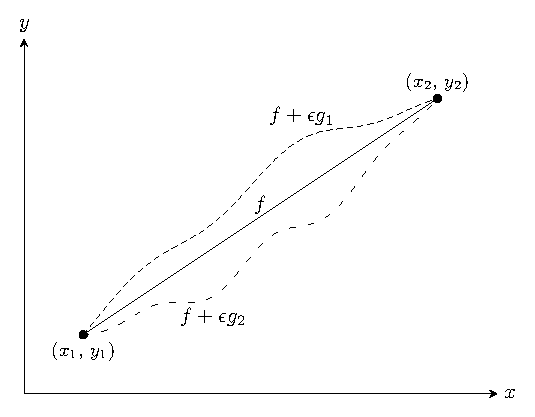
\includegraphics[keepaspectratio, width = 4.0 in]{images/shortest_path}
    \caption{The shortest path between two points ($x_1$, $y_1$) and 
            ($x_2$, $y_2$) is indicated by the solid curve $f$.  Two possible
            curves for arbitrary $g$ are also given.}
    \label{fig:shortest_path}
\end{figure} 

Taking the first variation of $F$,
\begin{equation}
\begin{split}
\delta F[f,g] &= \left ( \frac{d}{d\epsilon}\int^{x_2}_{x_1} 
                         \sqrt{1 + (f'(x)+\epsilon g'(x))^2} dx \right ) 
                 \Bigg |_{\epsilon=0} \\
              &= \left ( \int^{x_2}_{x_1} 
                         \frac{(f'(x)+\epsilon g'(x))g'(x)}
                              {\sqrt{1 + (f'(x)+\epsilon g'(x))^2}} \right ) 
                 \Bigg |_{\epsilon=0} \\
              &= \int^{x_2}_{x_1} \frac{f'(x)g'(x)dx}{\sqrt{1 + (f'(x))^2}} \, ,
\end{split}
\end{equation}
we find that the arc length is minimized when
\begin{equation}
 \delta F[y,g] =
   \int^{x_2}_{x_1}\frac{f'(x)g'(x)}{\sqrt{1 + (f'(x))^2}} = 0 \, .
 \label{eq:exampleprinciple}
\end{equation}
In this form, we can't say anything about $f$ or $g$.  Instead, we use 
integration by parts to go from $f'$ and $g'$ to $f''$ and $g$, and
Eq. \ref{eq:exampleprinciple} becomes
\begin{equation}
 \delta F[f,g] =
   \left [ \frac{f'(x)g(x)}{\sqrt{1 + (f'(x))^2}} \right ]^{x_2}_{x_1} - 
   \int^{x_2}_{x_1} \frac{f''(x)g(x)dx}{(1 + (f'(x))^2)^{\frac{3}{2}}} = 0\, .
 \label{eq:exampleprinciple2}
\end{equation}
While $g(x)$ is arbitrary \textit{between} $x_1$ and $x_2$, we must have 
$g(x_1) = g(x_2) = 0$ to that $f(x_1) = y_1$ and $f(x_2) = y_2$.  Thus, the 
first term of Eq. \ref{eq:exampleprinciple2} vanishes. 
By inspection, the second term vanishes for 
arbitrary $g$ only if $f'' = 0$.  This relation is known as 
the \textit{Euler equation}\footnote{In general, setting the first variation 
to zero gives rise to a set of partial differential equations collectively 
known as the Euler equations.}.  Of course, to satisfy $f''=0$ requires 
our solution to be of the form $Ax+B$, as expected.

%------------------------------------------------------------------------------%
\section*{A Variational Principle for Fixed Source Problems}

Suppose we are interested in a linear functional of the flux, such 
as $G_{\text{fs}}[\psi] = \langle \psi, \Sigma_d \rangle$, a reaction rate. 
An appropriate variational principle is represented by 
the \textit{generalized Roussopoulos functional}
\begin{equation}
 F_{\text{fs}} [\psi,\psi^*] = 
   G_{\text{fs}}[\psi] + \langle \psi^*, (Q-L\psi) \rangle \, .
\end{equation}
Note, $\delta F_{\text{fs}}[\psi,\psi^*] = 0$ is a variational principle 
for $G_{\text{fs}}$ if the corresponding solution $\psi$ 
yields $F_{\text{fs}}[\psi,\psi^*] = G_{\text{fs}}[\psi]$.  We see this is 
so when the second term of $F$ vanishes when $\psi$ solves $L\psi = Q$, i.e. 
when $\psi$ is the solution to the transport equation.

To determine the variational principle, we take the first variation 
of $F_{\text{fs}}$,
\begin{equation}
 \begin{split}
  \delta F_{\text{fs}} & [\phi,\phi^*] \\
   &= \left ( \frac{d}{d\epsilon} 
            \left ( \langle (\phi+\epsilon \delta \phi) \Sigma_d \rangle + 
                    \langle (\phi^* + \epsilon \delta \phi^*), 
                            (Q-L(\phi+\epsilon \delta \phi)) \rangle 
            \right ) 
    \right ) \Bigg|_{\epsilon=0} \\
   &= \langle \delta \phi, \Sigma_d \rangle - 
      \langle \phi^*,L \delta \phi \rangle + 
      \langle \delta \phi^*, Q \rangle - 
      \langle \delta \phi^*, L \phi \rangle +
      \mathcal{O}(\epsilon^2) \, .
 \end{split}
\end{equation}
Noting 
$\langle \phi^*,L\delta \phi \rangle = \langle L^* \phi^*,\delta \phi \rangle$, 
we have for our principle 
\begin{equation}
 0 = \langle \delta \phi, (\Sigma_d - L^* \phi^*) \rangle + 
     \langle \delta \phi^*, (Q-L\phi) \rangle \, ,
\end{equation}
which is satisfied when $L\phi = Q$ and $L^* \phi^* = \Sigma_d$.  These are 
the corresponding Euler equations, and we see they are just the original 
forward and adjoint transport equations.

The importance of this variational principle (and others in general) is that 
it gives us an estimate for $G_{\text{fs}}$ accurate to second order for 
approximate fluxes $\phi$ and $\phi^*$.  To demonstrate this, suppose the 
true solutions to the Euler equations are $\psi$ and $\psi^*$.  
Let $\phi = \psi + \delta \psi$ and $\phi^* = \psi^* + \delta \psi^*$.  
We subsitute these expressions into $F$ and find
\begin{equation}
 \begin{split}
    F_{\text{fs}} [\phi,\phi^*] &= 
      \langle \Sigma_d, (\psi+\delta \psi) \rangle + 
      \langle (\psi^*+\delta \psi^*),(Q-L(\psi+\delta \psi^*) \rangle \\
    &= \langle \Sigma_d,\psi \rangle + 
       \langle \Sigma_d, \delta \psi \rangle + 
       \langle \psi^*,Q \rangle + 
       \langle \delta \psi,Q \rangle  \\ 
    &- \langle \psi^*, L\psi \rangle - 
       \langle \psi^*, L\delta \psi \rangle - 
       \langle \delta \psi^*, L\psi \rangle - 
       \langle \delta \psi^*, L\delta \psi \rangle \\
    &= \langle \Sigma_d, \psi \rangle - 
       \langle \delta \psi^*, L\delta \psi \rangle \\
    &= G_{\text{fs}}[\psi] + \mathcal{O}(\delta^2) \, .
 \end{split}
 \label{eq:secondorderfs}
\end{equation}
Hence, $F$ provides a first order accurate (i.e. good through first order) 
estimate of the reaction rate given approximate forward and adjoint fluxes.

\section*{A Variational Principle for Eigenvalue Problems}

For eigenvalue problems, an appropriate functional is 
the \textit{Rayleigh quotient}
\begin{equation}
 F_{\text{ev}}[\psi,\psi^*] = 
   \frac{\langle \psi^*,L\psi \rangle}{ \langle \psi^*, F \psi \rangle } \, .
 \label{eq:rayleigh}
\end{equation}
Here, the quantity of interest is $G_{\text{ev}} = \lambda$, and, unlike the 
fixed source case, we have $G_{\text{ev}} = F_{\text{ev}}$.  You should show 
that $F_{\text{ev}}$ is in fact a valid expression for $\lambda$.  The 
associated Euler equations are just the forward and adjoint eigenvalue 
equations, which can be shown by setting the first variation 
of $F_{\text{ev}}$ to zero, an exercise left to the reader.
For approximate fluxes $\phi$ and $\phi$
\begin{equation}
 F_{\text{ev}}[\phi,\phi^*] = \lambda + \mathcal{O}(\delta^2) \, ,
\end{equation}
the proof of which is also left as an exercise.

\section*{Perturbation Theory from Variational Principles}

In general, it is possible to find first order perturbation estimates using 
the expression
\begin{equation}
 \delta = \bar{F}[\psi,\psi^*] - F[\psi,\psi^*] \, ,
 \label{eq:pertfromvar}
\end{equation}
where $F$ is the appropriate functional with nominal operators 
and $\bar{F}$ is the function evaluated with perturbed operators.  It must 
be stressed that $\psi$ and $\psi^*$ are assumed to be the exact fluxes for 
the unperturbed problem.

As an example, we re-derive the first order perturbation to a detector 
response.  Suppose the perturbations to our system 
include $L+\delta L$, $Q+\delta Q$, 
and $\Sigma_d + \delta \Sigma_d$.  Then Eq. \ref{eq:pertfromvar}  gives
\begin{equation}
\begin{split}
 \delta_{\text{fs}} &= \bar{F}[\psi,\psi^*] - F[\psi,\psi^*] \\
        &= \langle \psi, (\Sigma_d+\delta \Sigma_d) \rangle + 
           \langle \psi^*,(Q+\delta Q-(L+\delta L)\psi ) \rangle - 
           \langle \psi, \delta \Sigma_d \rangle \\
        &= \langle \psi,\delta \Sigma_d \rangle + 
           \langle \psi^* , \delta Q \rangle - 
           \langle \psi^*,\delta L \psi \rangle \, .
\end{split}
\label{eq:fixedpertvar}
\end{equation}
The last line is equivalent to Eq. \ref{eq:fixedpertresp} with the addition 
of the first term, which explicitly accounts for changes in the detector 
response function.

Eq. \ref{eq:pertfromvar} can also be applied to the Rayleigh quotient, 
yielding Eq. \ref{eq:eigenpertresp}, proof of which is left 
as an exercise.

%------------------------------------------------------------------------------%
\section*{Further Reading}

Most of the material presented here is contained in Chapter 7 of 
Duderstadt and Martin \cite{duderstadt1976tt}  in addition to Chapter 1 
of Stacey \cite{stacey1974vmn}.  The former contains several examples 
and a variational derivation of the diffusion equation.  The reader is 
also encouraged to look up Pomraning's large body of work on variational 
methods\footnote{It is worth noting that Stacey and Pomraning, both with 
prolific work in variational methods, did their graduate work in 
this department.}.

%------------------------------------------------------------------------------%
\begin{exercises}

  %----------------------------------------------------------------------------%
  \item \textbf{Second Order Accuracy}. 
    Show that the Roussopoulos functional $F[\phi,\phi^*]$ gives a second 
    order accurate value for $\langle \psi,\Sigma_d \rangle$ when $\phi$ 
    and $\phi^*$ are approximate values of $\psi$ and $\psi^*$, i.e. 
    prove Eq. \ref{eq:secondorderfs}.

  %----------------------------------------------------------------------------%
  \item \textbf{Fixed Source Perturbation}. 
    Prove Eq. \ref{eq:fixedpertvar}.
 
  %----------------------------------------------------------------------------%
  \item \textbf{Rayleigh Quotient}. 
    \begin{enumerate}[a.]
      \item Take the first variation of the Rayleigh quotient with respect to 
            the forward and adjoint fluxes and show the stationarity conditions 
            are just the forward and adjoint eigenvalue problems. 
      \item Demonstrate that the Rayleigh quotient is a second order 
            estimator for $\lambda$.
    \end{enumerate}

  %----------------------------------------------------------------------------%
  \item \textbf{Losses-to-Gains}. 
    Directly from the eigenvalue equation, we find 
    \begin{equation*}
      \lambda = (L\psi)/(F\psi) \, ,
    \end{equation*}
    a compact way to define losses-to-gains.  
    \begin{enumerate}[a.]
      \item Show why this is not a variational principle for $\lambda$.
      \item Consider again Eq. \ref{eq:rayleigh}.  How does the adjoint change 
            the physical interpretation of gains-to-losses?
    \end{enumerate}

  %----------------------------------------------------------------------------%
  \item  \textbf{Eigenvalue Perturbation}. 
    Prove that $\bar{F}_R[\psi,\psi^+]-F_R[\psi,\psi^+]$ yields the first 
    order perturbation estimate for $\delta \lambda$ given 
    by Eq. \ref{eq:eigenpertresp}.

  %----------------------------------------------------------------------------%
  \item  \textbf{Applying Roussopoulos}. 
    Consider a 1-d, 1-speed diffusion problem in a slab of 
    width $2a$, $\Sigma_a = 0.022$, and $D = 0.14$. 
    \begin{enumerate}[a.]
      \item Solve for the exact scalar flux $\phi(x)$, using the 
            conditions $\phi(\pm a)=0$, and
            assuming a uniform source $Q(x) = 1$ and $a=1$.
      \item Compute the total absorption rate in the slab.
      \item Now, approximate the solution as 
            $\tilde{\phi}(x) = Ax^2 + Bx +C$ with the same maximum 
            and the same boundary conditions.  Compute the absorption rate  
            using $\tilde{\phi}(x)$.
      \item Finally, recalling the 1-d, 1-speed diffusion equation is 
            self-adjoint, use the Roussopoulos principle to compute the 
            absorption rate.  What can you conclude? 
    \end{enumerate}

  %----------------------------------------------------------------------------%
  \item \textbf{More Roussopoulos}. 
    For the same problem, estimate the total absorption rate if something 
    causes $\Sigma_a = 1.1$.  Be careful to consider the impact of the change 
    in $\Sigma_a$ on both $\Sigma_d$ and $L$.

  %----------------------------------------------------------------------------%
  \item \textbf{Approximating Escape from a Slab}. 
    Recall the escape probability $P_{\text{esc}}$ for a homogeneous 1-d slab, 
    the subject of 
    Chapter \ref{lec:analytical}, Problem \ref{itm:escapeprobability}.  
    Here, consider a discrete ordinates approximation using the 
    two point Gauss-Legendre quadrature and Mark boundary conditions
    for a 10 cm slab with $\Sigma_t = 10$ [1/cm].
    \begin{enumerate}[a.]
      \item Solve for $P_{\text{esc}}$ directly using the S$_{\text{2}}$ 
            approximation.
      \item Use a variational principle to improve 
            your estimate of $P_{\text{esc}}$. 
      \item Compare both values to the exact value.
    \end{enumerate}

\end{exercises}

\chapter{Computational Geometry for Transport}
\label{app:computational_geometry}

\section*{Quadratic Surfaces}

A 2-D quadratic (or second-order) surface is defined 
implicitly as
\begin{equation}
 f(x, y) = A x^2 + B y^2 + C xy + Dx + Ey + F \, .
\end{equation}
 
For points \emph{on the surface}, $f=0$, and for points outside/inside the 
surface, $f \gtrless 0$.
 
Let 
\begin{equation*}
 \mathbf{r} = [x, y, 1]^{\transp} 
 \quad \text{and} \quad
 \mathbf{M} =
 \left [ 
 \begin{array}{ccc}
  2 A &   D  &   E   \\
    D & 2 B  &   C   \\
    E &   C  & 2 F   \, .
 \end{array}
 \right ]  
\end{equation*}
Then,
\begin{equation}
 f(x, y) = \frac{1}{2} \mathbf{r}^{\transp} \mathbf{M} \mathbf{r} \, .
\label{eq:quadratic_residual}
\end{equation}
\emph{ Prove this to yourself!}

\section*{Tracking Particles}


\emph{ Common problem}: \emph{where does a ray intersect a surface?}

Let a ray $\mathbf{r}$ be defined as 
\begin{equation}
 \mathbf{r} = \mathbf{r}_0 + t \mathbf{d}
\end{equation}
where $\mathbf{r}_0$ is some starting point, $\mathbf{d}$ is some 
direction (so $|\mathbf{d}|=1$), and $t$ is the distance from 
the starting point along the direction.

\vfill
Substitute this ray into \EQ{quadratic_residual} to find 
where the ray intersects the surface (and, hence, $f=0$).
The result is (\emph{ show this!})
\begin{equation}
  t^2 \overbrace{\mathbf{d}^{\transp} \mathbf{M} \mathbf{d}}^{a}
  + t \overbrace{\mathbf{r_0}^{\transp} \mathbf{M} \mathbf{d}}^{b}
  +   \overbrace{\mathbf{r_0}^{\transp} \mathbf{M} \mathbf{r_0}}^{c} = 0 \, ,
\end{equation}
which is quadratic in $t$.  If  
\begin{equation*}
  \begin{array}{cc}
      b^2 > 4ac & \text{there are two intersections} \\
      b^2 = 4ac & \text{there is one intersection (tangent)} \\
      b^2 < 4ac & \text{there are no intersections} 
  \end{array}
 \, . 
\end{equation*}


\section*{Creating Geometries}

Detran's computational geometry consists of \emph{ regions} 
defined by combinations of \emph{ nodes}. 

 

A \emph{ node} can be a  surface (called a \emph{ primitive}), 
an \emph{ operator} between two nodes (e.g., \emph{ union} and 
\emph{ intersection}), or a \emph{ translation} of another 
node.

 
It would be useful to simplify what is presented here using 
Python (but still without function implementations).  Ultimately,
all of the note presented so far will be typeset as formal
lectures, and I'd like one solid set of Python routines to 
form the core.


\chapter{Criticality Safety}
\label{lec:criticalitysafety}

In this lecture, we discuss the topic of \textit{criticality safety}, one 
of the most important physics-oriented aspects of nuclear engineering not 
specifically dealing with core physics, beginning with a brief  
overview.  Thereafter, the chief physical concerns related to criticality 
safety are described and illustrated with a simple example, and a few 
notable 
accidents over the past several decades are described.  Finally, 
computational aspects of criticality safety are discussed, and the topic 
of burnup credit is used as a case study to illustrate recent efforts in 
criticality safety analysis.

%------------------------------------------------------------------------------
% OVERVIEW
%------------------------------------------------------------------------------

\section*{Overview}

\textit{Nuclear criticality safety}, 
as defined by the American National Standard ANSI/ANS 8.1 \cite{ans8.1}, is 
the ``protection against the consequences of a criticality safety
accident, preferably by prevention of the accident,'' and it defines
a \textit{criticality accident} as ``the release of energy as a 
result of accdental production of a self-sustaining or
divergent neutron chain reaction.''

ANSI/ANS 8.1 provides general guidance for 
nuclear criticality safety applied to fissionable materials \textit{outside} 
of reactors.  In addition to ANSI/ANS 8.1, a number of more specialized 
standards exist, a few of which are 
summarized in Table \ref{tbl:ansstandard}. The interested 
student can request these standards from the library, but they tend to be 
expensive (and, admittedly, rather dry reading).  ANSI/ANS 8.1 has been
put on the 22.106 Stellar site.

\begin{table}[ht]
    \caption{Several ANSI/ANS Standards Applicable to Criticality Safety.}
    \begin{center} 
    \begin{tabular*}{1.00\textwidth}{@{\extracolsep{\fill}} p{3cm}p{0.9\textwidth-3cm} } 
      \toprule 
	Number-Revised    &  Title \\
      \midrule
       8.1-1998                  &  Nuclear Criticality Safety in Operations 
                                    with Fissionable Materials Outside 
                                    Reactors \\
       8.3-1997                  &  Criticality Accident Alarm System \\
       8.5-1996                  &  Guide for Nuclear Criticality Safety in 
                                    the Storage of Fissile Materials \\
       8.17-2004                 &  Criticality Safety Criteria for the 
                                    Handling, Storage, and Transportation 
                                    of LWR Fuel Outside Reactors \\
       8.24-2007                 &  Validation of Neutron Transport 
                                    Methods for Nuclear Criticality Safety 
                                    Calculations \\
       8.27-2008                 &  Burnup Credit for LWR Fuel \\
      \bottomrule 
    \end{tabular*} 
    \end{center} 
    \label{tbl:ansstandard}
\end{table}

The Nuclear Regulatory Commision (NRC) also offers guidance with 
respect to criticality safety.  NRC documents are most often found in 
the NUREG series, published by the NRC itself, by contractors, or through
international agreements.  

Additionally, the NRC provides \textit{regulation} through relevant 
portions of the Code of Federal Regulations (CFR).  Both DOE and NRC
share regulations under title 10, \ie those regulations beginning
with 10CFR.\footnote{That DOE and NRC share the same title is most likely
due their common origin: the Atomic Energy Commision.}
The parts of 10CFR most relevant to criticality safety are 10CFR-0, 1, 2,
20, and several between 50 and 75.  As an exercise, the student is
encouraged to find one or more of these regulations (or NUREG documents)
related to criticality safety and explain its relevance.

As a historical note, nuclear criticality safety as a discipline is 
about as old as other nuclear 
engineering areas; it began with the large scale chemical processing at
the K-25 gasseous diffusion plant in Oak Ridge, TN and the Hanford, WA site, 
both major components of the 
Manhatten Project.  Of course, the initial work at Los Alamos generated 
much knowledge before the larger scale projects were begun, and in fact, 
it was a young Richard Feynman who carried much of that experience from 
Los Alamos to Oak Ridge in 194X at the bequest of Oppenheimer 
\cite{something}. In Feynman's own words, he was told by Oppenheimer to
tell the Oak Ridge folks (stubborn military types), ``Los Alamos cannot 
accept the responsibility
for the safety of the Oak Ridge plant unless they are full informed as
to how it works.''  He delivered the message, and when they agreed to 
listen, he
``told them all about neutrons, how they worked, da da, ta ta ta,
there are too many neutrons together, you've got to keep the material
apart, cadmium absorbs \ldots'' and so forth.  The Oak Ridge folks
went back to the design board, and a ``practice'' was born.

%------------------------------------------------------------------------------
% PHYSICAL CONCERNS
%------------------------------------------------------------------------------

\section*{Physical Concerns}

When we analyze a system for criticality safety, what are the important 
characteristics the system?  An analyst must understand \textit{what} to
analyze before computational techniques become useful.

Several features can be intuited by any
student of reactor physics: the more fissile material one has, the easier
it is to achieve criticality.  That means increased 
\textit{mass}, \textit{concentration}, \textit{enrichment}, or 
\textit{volume} of a fissile material should bring
a system closer to criticality (or past it, unfortunately).

But there are other factors: what neutrons do we like in our typical light
water reactors?  Thermal ones, of course, and to get those, we need 
\textit{moderation}.  Moreover, those same reactors feature a layer of
water around the periphery, which \textit{reflect} neutrons back into
the core.  To reduce power in a reactor (or to shut it down), we insert
some level of \textit{absorption} via control rods, which limits
the \textit{interaction} of fissile assemblies with one another. 

These key chacteristics, easily remembered via the acronym 
MAGICMERV \cite{handbook}, are equally applicable to nuclear
criticality safety.  


%------------------------------------------------------------------------------
% ACCIDENTS
%------------------------------------------------------------------------------

\section*{Accidents}

What exactly \textit{is} a criticality accident?  In the simplest terms,
it is an excursion, an uncontrolled chain reaction.  To help understand
accidents
both qualitatively and quantitatively, let's review a few ideas from
reactor kinetics.  Recall that \textit{reactivity} measures a departure
from criticality, and is most often expressed via
\begin{equation}
 \rho = \frac{k-1}{k} \, .
\end{equation}
Postive $\rho$ denotes a supercritical state, negative $\rho$ a 
subcritical state, and $\rho = 0$ is equivalent to $k=1$ or a 
critical state.  We can further differentiate between a \textit{delayed
critical} state and a \textit{prompt critical} state.  The latter 
occurs when $\rho > \beta$, where $\beta$ is the delayed neutron
fraction.  This situation is to be avoided in all but a few specific
experimental situations, for in the prompt critical regime, 
the growth of the neutron population occurs on timescales close
to the prompt neutron lifetime (say $10^{-8}$ to $10^{-4}$ seconds in many
systems of interest).  

To get an idea of the orders of magnitude we deal with in an accident
situation, consider a critical system with a constant neutron population
of just one neutron.  Suddenly, a perturbation brings the system
into a prompt critical state for a short time $\Delta t$.  During this
time, the population grows as $n \propto n_o e^{(\rho-\beta)t/\Lambda}$.  
Assuming $\Lambda = 10^{-5}$ seconds, $\rho-\beta = 0.002$, and the perturbation 
lasts two tenths of second\footnote{the average human reaction time is
about 200 milliseconds. 
See \url{http://www.humanbenchmark.com/tests/reactiontime/stats.php}}, 
we estimate that the number of neutrons produced is 
roughly
\begin{equation}
\begin{split}
 N &= \int^{0.5}_0 dt e^{(\rho-\beta)t/\Lambda} \\
   &= \frac{10^{-5}}{0.002} (e^{40} - 1) \\
   &\approx 1 \cdot 10^{15} \, .
\end{split}
\end{equation}
Suppose a worker is about a half a meter from the neutron source, so that
the fluence is $\Phi \approx 10^{15} / (4\cdot \pi \cdot 50^2)$ n/cm$^2$.
Looking up neutron fluence-to-dose equivalent factors (see 10CFR-20
\footnote{\url{http://www.nrc.gov/reading-rm/doc-collections/cfr/part020/part020-1004.html}}) 
suggests
that a high energy (1 MeV) fission fluence of $27\cdot 10^6$  n/cm$^2$
corresponds
to a dose of 1 rem.  Hence, our excursion yields a dose of around
1200 rem (12 Sv).  For perspective, a dose of 4 Sv is lethal roughly 
half the time.  Of course, this is a crude example, but it gives a 
very clear picture of the issues at hand.

In fact, the example above is not too far different than one of the first
documented criticality accidents from August of 1945.
Figure \ref{fig:pu_sphere} shows
a 6.2 kg plutonium sphere coated with nickel and surrounded by
blocks of tungsten carbide for reflection.  In the accident, an 
experimenter was placing blocks to achieve criticality.  While
placing the last block, the detector reading suggested that 
the block would actual produce a supercritical state.  Unfortunately,
the experimenter dropped the brick onto the assembly, yielding
a prompt supercritical excursion of $10^{16}$ fissions
before he was able to remove the brick.  A later study estimated
the resulting dose to be 510 rem, which proved to be fatal some
28 days later.  The same assembly would be involved in a second
fatal accident just months later, where the experimenter handled
one of two beryllium hemisphere reflectors
 with his thumb (in a hole in the 
hemisphere) and a screwdriver, a procedure Feynman dubbed
``tickling the dragon's tail.''   The screwdriver, holding the 
reflectors apart, slipped and caused an excursion that led to 
the experimenter's death 9 days later and significant doses
to observers.

\begin{figure}[ht] 
    \centering
    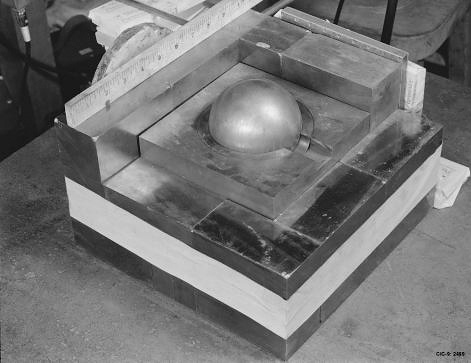
\includegraphics[keepaspectratio, width = 5.0 in]{images/pu_sphere}
    \caption{Plutonium sphere reflected by tungsten-carbide bricks.}
    \label{fig:pu_sphere}
\end{figure}

A second type of accident involves processing operations in which
fissile materials are in solution.  The first domestic processing
accident occured at the Y-12 plant in Oak Ridge, TN.  Y-12 
produces parts from HEU for use in nuclear weapons.  

The accident occured in a portion of the plant used to 
recover HEU from waste material and place it in tanks of favorable
geometry.  These tanks were to be emptied, cleaned, and leak-tested 
with water.  Before the leak-testing began, however, uranium 
solution had leaked from the process stream into the piping
below the storage tanks (and actually into one of the tanks,
as its release valve had been let open).  When the other tanks, full
of water, were emptied, the uranium solution and water accumulated
in a 55 gallon drum.  A nearby worker first noticed dark yellow
fumes followed by a blue flash.  Eight workers received significant
doses, though none died as a result of acute effects.

A rather complete history of criticality accidents in the U.S. and
around the world is contained in the latest edition of
 \textit{A Review of Criticality Accidents} from Los Alamos.  This
document is a really great piece of nuclear history, and students
are highly encouraged to skim through the many accidents covered.

%------------------------------------------------------------------------------
% Computational Aspects
%------------------------------------------------------------------------------

\section*{Computational Aspects}

The intent of this section to provide the reader with an 
overview of criticality safety analysis validation. A brief 
review of regulations and guidance pertinent to criticality safety of 
fissile materials outside reactors is given, with a particular emphasis on 
requirements for ensuring subcritical conditions. The traditional approach to 
bias determination is discussed, and one specific method used in practice
is described and demonstrated in an illustrative example. Subsequently, 
modern S/U-based validation techniques are discussed, and an 
illustrative example is provided and related to the traditional approach.

%------------------------------------------------------------------------------

\subsubsection{Subcritical Limits}

As noted above, ANSI/ANS-8.1 provides guidance 
for avoiding criticality accidents during handling of fissionable material 
outside of reactors \cite{ans8}. The standard provides basic safety principles 
in addition to several limits for simple systems of single isotopes.  
Specifically, the standard defines a \textit{subcritical limit} to be ``the 
limiting value assigned to a controlled parameter that results in a subcritical 
system under specified conditions. The parameter limit allows for 
uncertainties in the calculations and experiemental data used in the derivation 
but not for contingencies.''

These limits are \textit{absolute maxima}, and since they do not include 
contingencies, in practice, adminstrative margins are employed.  A typical 
value, as we'll see below, tends to be 5\% on \keff.

Table \ref{tbl:controlparams} gives several examples of single control 
parameters used in criticality safety analysis.  Note, while ANSI/ANS 8.1 
specifies limits in terms of a single parameter, in some cases, multiple 
parameter limits are also employed.  The standard suggests a few examples, and
cites the technical literature for further guidance. However, while less 
conservative, multiple 
parameter limits require additional adminstrative margins and may be harder to 
use in validation.

\begin{table}[ht]
    \caption{Example single parameters and subcritical limits.}
    \begin{center} 
    \begin{tabular*}{0.90\textwidth}{@{\extracolsep{\fill}} ll } 
      \toprule 
	parameter &  example limit \\
      \midrule
       fissile mass                    &  0.78 kg ${}^{235}$U in UO$_2$NO$_3$ \\
       dimension (width, volume, etc.) &  6.2   L ${}^{235}$U in UO$_2$NO$_3$ \\
       concentration                   &  11.6 g/L${}^{235}$U in UO$_2$NO$_3$ \\
       enrichment                      &  5\%     ${}^{235}$U in UO$_2$       \\
       fissile mass                    &  20.1 kg ${}^{235}$U in UO$_2$ 
                                          (w/ $\rho \leq 18.81$ g/cc) \\
      \bottomrule 
    \end{tabular*} 
    \end{center} 
    \label{tbl:controlparams}
\end{table}

%------------------------------------------------------------------------------


\subsection*{Criticality Safety Analysis Validation}

While the single parameter limits provide useful guidance, two questions 
naturally arise.  First, how does one actually establish these limits?  And 
second, how does one ensure subcriticality in systems that are much more 
complex than, for example, a sphere?  The answer in both cases is by using 
computational methods validated against experiment.

In addition to the single parameter limits, ANSI/ANS-8.1 provides 
requirements for ensuring computational methods used in criticality safety 
analyses are both valid and within the ``area of applicability'' for specific 
applications. The standard defines the area of applicability as ``limiting 
ranges of material compositions, geometric arrangements, neutron energy 
spectra, and other relevant parameters \ldots within which the bias of the 
calculational method is established'' \cite{ans8}.  In other words, an 
\textit{application} is the system of interest, such as a spent fuel canister 
for shipment and disposal. A computational method is \textit{applicable} if 
it is verified against a set of \textit{experiments} that are similar to the 
application with respect to composition, geometry, and so forth.

A \textit{computational bias} is the systematic 
discrepancy between and experimental data and calculated results. Biases 
have associated uncertainties, which quantify the accuracy and 
precision of calculated values and the uncertainty in measured data.

When computational tools are used in criticality safety analyses, the standard
requires that the bias be established.  Qualitatively, the bias must be 
determined via correlating data from critical experiments to computational 
models of the same experiments using the tool to be validated. 
Typically, the measured and 
computed values of \keff are related, but other physical quantities may 
also be used.  The bias is used to normalize a particular code within its 
area of applicability so that its results, after applying the bias, may be 
used to predict criticality within the bias uncertainty.

Another American National Standard, ANSI/ANS-8-17, further explicates 
use of computational tools by defining specific criteria for establishing 
subcriticality \cite{ans8_17}.  Whenever computational methods are 
used in criticality safety analyses, the standard requires that the calculated 
application multiplication factor $k_a$ must be less than or equal to the 
allowable multiplication factor.

The easiest way to think of this is to note that the largest, ``worst case'' 
value for $k_a$ must be below the smallest, least conservative computed 
estimate.  That is to say, the maximum expected application multiplication 
factor (\ie $k_a + \Delta k_a$) must be less than the minimum expected 
computed value (\ie $k_c - \Delta k_c$) for an applicable critical experiment, 
\ie a real, measured system whose \keff is unity, or an average computed 
\keff for several such experiments.  Mathematically, this can be written as
\begin{equation}
 k_a + \Delta k_a \leq k_c - \Delta k_c \, ,
\end{equation}
or
\begin{equation}
 k_a \leq k_c  - \Delta k_a - \Delta k_c \, .
\end{equation}
For added conservatism, the standard further requires that
\begin{equation}
 k_a \leq k_c - \Delta k_a - \Delta k_c - \Delta k_m \, ,
\label{eq:kapp}
\end{equation}
where the standard defines:

\begin{tabular}{rp{10cm}}
 $k_a$           & is the calculated \keff of the 
                   application system for all normal or credible 
                   abnormal conditions; \\
\end{tabular}

\begin{tabular}{rp{10cm}}
 $k_c$           & is the average \keff from the calculation of 
                   the benchmark criticality experiments. 
                   The experiments used 
                   should be neutronically similar to the application
                   system. If the application system has 
                   parameters beyond the area of applicability established 
                   by the benchmark experiments, then the area of 
                   applicability
                   may be extended using trends in the calculated values 
                   of $k_c$ as functions of those parameters; \vspace{12pt} \\
\end{tabular}

\begin{tabular}{rp{10cm}}
 $\Delta k_a$    & is an allowance for 
                 \begin{itemize}
                   \item statistical or convergence uncertainties in 
                         the computed $k_a$;
                   \item material and fabrication tolerances;
                   \item uncertainties due to geometry or material
                         simplifications and approximations;
                 \end{itemize}  \\
\end{tabular}

\begin{tabular}{rp{10cm}}
 $\Delta k_c$    & is a margin for uncertainty in $k_c$ that includes 
                   allowances for
                 \begin{itemize}
                   \item uncertainties in the critical experiments;
                   \item statistical or convergence uncertainties
                         in the computated $k_c$;
                   \item uncertainties due to extrapolation of $k_c$ 
                         outside the experimental data range;
                   \item uncertainties due to geometry or material
                         simplifications and approximations;
                 \end{itemize}
\end{tabular}

\begin{tabular}{rp{12cm}}
 $\Delta k_m$    & is an arbitrary ``administrative'' 
                   margin to ensure the subcriticality 
                   of $k_a$. \\
\end{tabular}

Eq. \ref{eq:kapp} can be rewritten as
\begin{equation}
 k_a + \Delta k_a + \Delta k_m - \beta + \Delta \beta \leq 1 \, ,
\label{eq:kallow}
\end{equation}
where $\beta = k_c - 1$ is the bias and $\Delta \beta = \Delta k_c$ is the 
uncertainty in the bias.  The definition of $\beta$ is based on the fact 
that critical experiments, by their definition, have \keff = 1, and hence 
the bias is just the difference between the computed value and unity.  By 
convention, the bias is defined such that a \textit{ negative} $\beta$ 
indicates an \textit{ underestimated} \keff\!, which is undesirable.

To ensure subcriticality in the application system, an \textit{ upper 
subcritical limit} is defined as
\begin{equation}
 USL = 1 - \Delta k_m + \beta - \Delta \beta \, ,
\label{eq:usl}
\end{equation}
and from Eq. \ref{eq:kallow}, it is apparent that $k_a + \Delta k_a \leq USL$ 
\cite{lichtenwalter1997cbg}.   Thus, the USL is the maximum value an 
application \keff (plus any uncertainties) may have for which the 
application can, with a high degree of confidence, be considered 
subcritical.  The value $1 - USL$  is the mathematical definition of the 
subcritical margin.  In the event the bias $\beta$ is positive, \ie the 
computed value $k_c$ overestimates \keff\!, current practice is to set 
the bias to zero rather than reduce the subcritical margin.

%------------------------------------------------------------------------------

\subsubsection{Traditional Bias Determination}

In the United States, biases and associated uncertainties and USL's have 
often been found through use of \textit{ trending analysis}.  A suite of 
critical experiments is selected for use in a specific safety analysis 
based on the similarity of the experiments to the safety analysis system.  
Traditionally, this similarity is based on physical parameters that include 
the fissile material, hydrogen-to-fissile atom ratio (H/X), average neutron 
energy group causing fission, and energy of average lethargy causing 
fission (EALF), among others \cite{broadhead2004sau}.

While various methods using trending analysis exist for determining the 
biases and USL's, one common approach, denoted USL$_1$ in the 
literature \cite{broadhead2004sau}, is discussed here to provide at least 
some background of current practice. The following description is largely 
adapted from the technical report in which it was first developed 
\cite{lichtenwalter1997cbg}. 

The method computes $k_c(x)$ as a function of a trending parameter $x$ 
using linear regression.  The bias, $\beta(x)$, is just $k_c(x) - 1$.  .  

A lower confidence band $w(x)$ is statistically computed using current 
experiments and uncertainties as well as a specified confidence.  This 
confidence band defines the value below which an additional computed 
\keff value (\ie not included in the analysis) must be for the additional 
system to be considered subcritical with a high degree of confidence.  
Equivalently, for a given value of the trending parameter $x$, $w(x)$ 
represents the value \textit{ above} which the additional computed value $k_c$ 
will be \textit{ if} the system in question is critical---and this consequently 
implies any negative $\beta(x)$ is no worse than $w(x) - 1$.  Hence, if our 
aim is to ensure the actual \keff of a system is subcritical, then its 
computed value should be \textit{ less} than the appropriate confidence band 
value.

To simplify analyses, the limiting width, $W$, of the confidence band is 
used, which (like $w(x)$) takes into account all uncertainties associated 
with the experiments (\eg experimental, stochastic, etc), and consequently, 
is a statistical measure of $\Delta \beta$.  The width $W$ of the 
confidence band is defined
\begin{equation}
 W = \mathrm{max} \Big \{ w(x) | x_{\mathrm{min}},x_{\mathrm{max}} \Big \} \, ,
\label{eq:confwidth}
\end{equation}
where
\begin{equation}
 w(x) = t_{1-\gamma} s_p \Bigg ( 1 + \frac{1}{n} + 
        \frac{(x-\bar{x})^2}{\sum^n_{i=1} (x_i - \bar{x})^2} \Bigg )^{1/2} \, ,
\end{equation}
and $n$ is the number of critical experiments included in the analysis, 
$t_{1-\gamma}$ is the student-t distribution statistic for $1-\gamma$ 
and $n-2$ degrees of freedom ($\gamma$ is the desired confidence level), 
$\bar{x}$ is the mean value of $x$ in the set of experiments, and $s_p$ 
is the pooled standard deviation for the set of calculations.

The pooled standard deviation $s_p$ is defined by
\begin{equation}
 s^2_p = s^2_{k(x)} + s^2_w \, ,
\end{equation}
where $s^2_{k(x)}$ is the mean-square error of the linear regression, 
defined as
\begin{equation}
 s^2_{k(x)} = \frac{1}{n-2} \Bigg ( \sum^n_{i=1} (k_i - \bar{k})^2 - 
              \frac{\Big(\sum^n_{i=1} (x_i-\bar{x})(k_i -\bar{k}) \Big )^2 }
                   {\sum^n_{i=1} (x_i - \bar{x})^2} \Bigg ) \, ,
\end{equation}
and $s^2_w$ is the variance of the data, defined as
\begin{equation}
 s^2_w = \frac{1}{n} \sum^n_{i=1} \sigma^2_i \, ,
\end{equation}
where  $\sigma_i$ is the uncertainty in the $i$th calculated value, 
accounting for method uncertainty (\eg Monte Carlo statistics) and 
estimated uncertainty due to cross-section uncertainty 
(see Section \ref{sec:uncanal}).

The width of the confidence $W$ is chosen to be the \textit{ maximum} value 
of $w$ at the limits of the range of $x$ corresponding to the experiments 
to be conservative, and moreover, it serves to simplify the definition of 
USL.  Current guidance is to define $W$ at the 95\% confidence level, 
\ie choose $\gamma = 0.95$.  See Section \ref{sec:exampletrends} below 
for an illustrative example of the USL$_1$ methodology.

%------------------------------------------------------------------------------

\subsubsection{S/U-Techniques}

Unfortunately, the proper selection of parameters over which to trend, 
and the experiments with which to trend, is largely based on expert 
judgement.  As experiments continue to become more expensive, use of 
computational methods will grow.  Furthermore, new applications will 
continue to extend beyond the areas of applicability of current 
experimental data, and consequently, methods to extend beyond these 
areas are needed.

For the past several years, ORNL has worked with the support of the 
NRC and the Department of Energy's (DOE) Nuclear Criticality Safety 
Program to develop ``a rigorous physics-based approach for the 
determination of system similarity'' for determining areas of 
applicability \cite{broadhead2004sau}.  Additionally, their efforts 
aimed to develop the methodology and computational tools needed for 
``determination of biases and uncertainties due to experimental 
descriptions, computational methods, and nuclear data.''

As an alternative to traditional trending analysis, work was done to 
develop S/U-based, easily-quantifiable parameters to measure the 
similarity of systems.  It is beyond our scope to describe the 
methods in detail.  Interested readers should see the exercises
of Lecture \ref{lec:the_adjoint_and_perturbation_theory} for some
basic theory needed to derive the results, and Ref. 
\cite{broadhead2004sau} for greater detail.

Skipping the theory, what we end up with is the sensitivity
of \keff to the various underlying nuclear data, 
\begin{equation}
 S_{k,\sigma_x} = \frac{\sigma_x}{k}\frac{\partial k}{\partial \sigma_x} 
 \label{eq:keffsens}
\end{equation}
where $x$ denotes some reaction of interest.  We express the sensitivity 
of \keff to all nuclides in a system as the vector $\mathbf{S}_k$,
which can implicitly represent dependence on multigroup data.

Sensitivity vectors can be used to compare both the qualitative and 
quantitative similarity between two systems with respect to single or 
several nuclide-reactions. Let the entire set of group-wise, nuclide-reaction 
cross-sections be denoted 
$\bm{\sigma} \equiv \sigma_i, \; \; n = 1,\;2,\ldots,N$, where $N$ is the 
total number of nuclide-reactions multiplied by the number of energy 
groups.  The $N\times N$ correlation (\ie relative covariance) matrix 
of $\bm{\sigma}$ is defined
\begin{equation}
\mathbf{C_{\sigma \sigma}} \equiv \Bigg[\frac{\mathrm{COV}(\sigma_i,\sigma_j)}
                                             {\sigma_i \sigma_j} \Bigg ] \, ,
\end{equation}
where $i$ and $j$ range from 1 to $N$, and 
\begin{equation}
\mathrm{COV} = \langle (\sigma_i - \bar{\sigma_i})(\sigma_j - 
               \bar{\sigma_j}) \rangle 
             = \langle \delta \sigma_i \delta \sigma_j \rangle \, ,
\end{equation}
where $\bar{\sigma_i}$ represents the expected value of the data $\sigma_i$.  

Because the components of \cov represent relative uncertainties, and because 
from above, we know the \keff sensitivity represents the relative change in 
\keff due to relative changes in some nuclide-reaction data, the relative 
uncertainty in \keff is therefore
\begin{equation}
\frac{\delta k}{k} = \sqrt{ \mathbf{S}_k \mathbf{C_{\sigma \sigma}} 
                     \mathbf{S}_k^T } \, ,
\end{equation}
where $T$ denotes the matrix transpose.  If several systems are of interest, 
then an $N \times I$  matrix of sensitivity vectors $\mathbf{\bar{S}}_k$ can 
be defined, where $I$ is the number of systems.  By folding 
$\mathbf{\bar{S}}_k$ with \cov, one obtains
\begin{equation}
 \mathbf{C}_{kk} =  \mathbf{\bar{S}}_k \mathbf{C_{\sigma \sigma}} 
                    \mathbf{\bar{S}}_k^T  \, ,
\label{eq:kunc}
\end{equation}
an $I\times I$ matrix consisting of each system's relative variance in 
\keff (\ie $(\Delta k/k)^2$) due to data uncertainties (the diagonal terms, 
$\alpha_{ii}$) and the relative covariances in \keff between systems 
(the off-diagonal terms, $\alpha_{ij}$).  These off-diagonal terms 
represent ``shared variance'' or ``shared uncertainty'' between systems.  

The correlation coefficient between system $i$ and $j$ is defined
\begin{equation}
 c_{k} =  \frac{\alpha^2_{ij}}{\alpha_i \alpha_j}  \, ,
\label{eq:ck}
\end{equation}
which, as is expected, takes on values between -1 
(completely anti-correlated) and 1 (completely correlated). 
A value $c_k = 0$ indicates no correlation between systems.  

The correlation of two systems is greatest if they share basic 
characteristics, \eg fuel type, moderator, other materials.  Two 
water-moderated thermal UO$_2$ systems would be expected to have 
a higher degree of correlation than would such a thermal system 
and a molten salt fast reactor.  Use of $c_k$ as a trending 
parameter in the USL$_1$ method is illustrated below.

%------------------------------------------------------------------------------

\subsubsection{Example Analyses}

To illustrate the USL$_1$ method using both traditional parameters 
and $c_k$, 25 thermal LEU systems were chosen for example analyses.  
Two additional systems were selected as ``applications'' for which 
the $\beta$, $\Delta \beta$, and the USL are determined\footnote{The 
minimum recommended number of experiments for trending with the 
USL$_1$ method is 25; here, just the minimum was used for these example 
cases.}. The experiments range from 2.35\% to 5\% enrichement, and have 
EALF values ranging from 0.017 to 2.24 eV.  %These parameters, along 
%with $c_k$ with respect to the two applications (LCT-079-002 and 
%LCT-050-001), are provided in Table \ref{tbl:exampletrend}. 
All experiments 
are included in the International Handbook of Evaluated Criticality Benchmark 
Experiments \cite{ihecsbe} and are low enriched uranium, thermal assemblies.
The LCT-079 and LCT-050 are experiments
of use to burnup credit, a topic discussed below; however, their use here
is purely for example.  

Figures \ref{fig:trend_ealf}-\ref{fig:trend_ck2} show the trending analysis 
for using EALF, enrichment, and $c_k$.  For both EALF and enrichment, only 
one analysis was needed for the applications since neither parameter depends 
on the application.  However, separate cases were run using $c_k$ values 
specific to the given application.  The experiments are the black dots, 
and the applications are red shapes.  For all cases, the uncertainty is 
computed using Eq. \ref{eq:kunc}, where the uncertainty for the system is 
its associated diagonal element of $\mathbf{C}_{kk}$, \ie the uncertainty 
in cross-sections propagated to \keff via use of sensitivity profiles.  
This is in line with previous analyses \cite{broadhead2004sau}.  Note, for 
the USL, an administrative margin of $\Delta k_m = 0.05$ was used.

% \begin{table}[hp]
%  \caption{Experiment and test application parameters.  Note (a) and (b) refer to the LCT-079 and LCT-050 experiments.}
%  \begin{center} 
%  \begin{tabular*}{0.95\textwidth}{@{\extracolsep{\fill}} ccccccc } 
%   \toprule 
%          Id.       &  \keff   & $\sigma_k$&  EALF (eV)&  Enrich.(\%) & $c_k$ (a) & $c_k$ (b)    \\ 
%    \midrule
%   LCT-010-005  &  0.9951  &  0.0050  &  3.89E-01  &  4.306  &  0.861  &  0.890  \\
%   LCT-010-016  &  0.9936  &  0.0058  &  2.92E-01  &  4.306  &  0.977  &  0.982  \\
%   LCT-010-017  &  0.9937  &  0.0058  &  2.86E-01  &  4.306  &  0.979  &  0.983  \\
%   LCT-010-018  &  0.9924  &  0.0058  &  2.81E-01  &  4.306  &  0.980  &  0.985  \\
%   LCT-010-019  &  0.9917  &  0.0058  &  2.74E-01  &  4.306  &  0.980  &  0.986  \\
%   LCT-017-003  &  0.9927  &  0.0055  &  9.57E-02  &  2.350  &  0.899  &  0.924  \\
%   LCT-017-004  &  0.9919  &  0.0052  &  2.17E-01  &  2.350  &  0.827  &  0.850  \\
%   LCT-017-005  &  0.9945  &  0.0053  &  1.89E-01  &  2.350  &  0.851  &  0.876  \\
%   LCT-017-006  &  0.9939  &  0.0054  &  1.78E-01  &  2.350  &  0.862  &  0.888  \\
%   LCT-017-007  &  0.9937  &  0.0053  &  1.69E-01  &  2.350  &  0.858  &  0.884  \\
%   LCT-042-001  &  0.9906  &  0.0054  &  1.73E-01  &  2.350  &  0.797  &  0.764  \\
%   LCT-042-002  &  0.9909  &  0.0055  &  1.79E-01  &  2.350  &  0.801  &  0.767  \\
%   LCT-042-003  &  0.9897  &  0.0054  &  1.86E-01  &  2.350  &  0.779  &  0.747  \\
%   LCT-042-004  &  0.9918  &  0.0054  &  1.84E-01  &  2.350  &  0.768  &  0.736  \\
%   LCT-042-005  &  0.9921  &  0.0057  &  1.81E-01  &  2.350  &  0.891  &  0.862  \\
%   LCT-049-001  &  0.9904  &  0.0057  &  2.02E+00  &  5.000  &  0.889  &  0.860  \\
%   LCT-049-002  &  0.9914  &  0.0057  &  2.03E+00  &  5.000  &  0.895  &  0.867  \\
%   LCT-049-003  &  0.9913  &  0.0055  &  2.15E+00  &  5.000  &  0.877  &  0.849  \\
%   LCT-049-004  &  0.9906  &  0.0058  &  2.24E+00  &  5.000  &  0.932  &  0.910  \\
%   LCT-049-005  &  0.9915  &  0.0059  &  1.14E+00  &  5.000  &  0.934  &  0.911  \\
%   LCT-049-006  &  0.9900  &  0.0055  &  1.15E+00  &  5.000  &  0.889  &  0.894  \\
%   LCT-049-007  &  0.9904  &  0.0053  &  1.11E+00  &  5.000  &  0.873  &  0.878  \\
%   LCT-049-008  &  0.9906  &  0.0053  &  1.19E+00  &  5.000  &  0.862  &  0.867  \\
%   LCT-049-009  &  0.9912  &  0.0053  &  7.39E-01  &  5.000  &  0.869  &  0.873  \\
%   LCT-049-010  &  0.9904  &  0.0053  &  7.47E-01  &  5.000  &  0.869  &  0.874  \\
%   \midrule
%   LCT-079-002  &  0.9897  &  0.0069  &  2.03E+00  &  4.310  &  1.000  &  na     \\
%   LCT-050-001  &  0.9906  &  0.0067  &  1.99E-01  &  4.738  &  na     &  1.000  \\
%   \bottomrule 
%  \end{tabular*} 
%  \end{center} 
%  \label{tbl:exampletrend}  
% \end{table}

\begin{figure}[htp] 
    \centering
    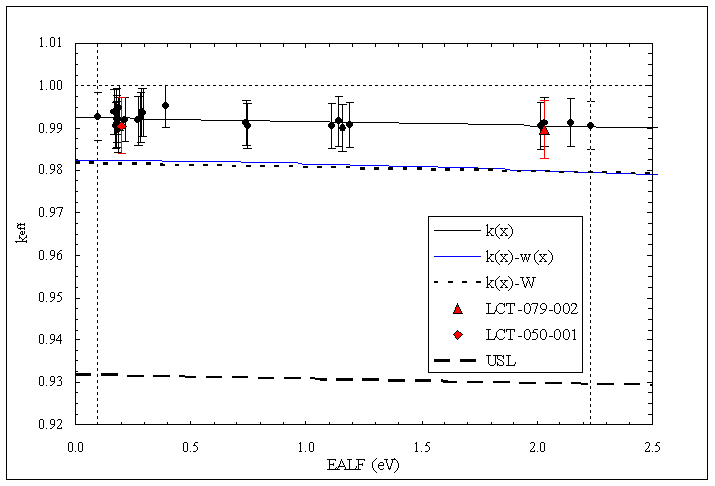
\includegraphics[keepaspectratio, width = 5 in]{images/trend_ealf}
    \caption{Example trending analysis using EALF.}
    \label{fig:trend_ealf}
\end{figure}


\begin{figure}[htp] 
    \centering
    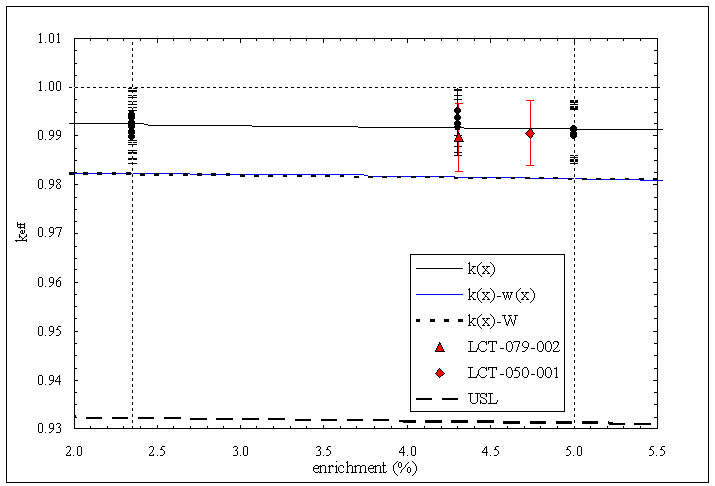
\includegraphics[keepaspectratio, width = 5 in]{images/trend_enrich}
    \caption{Example trending analysis using enrichment.}
    \label{fig:trend_enrich}
\end{figure}


\begin{figure}[htp] 
    \centering
    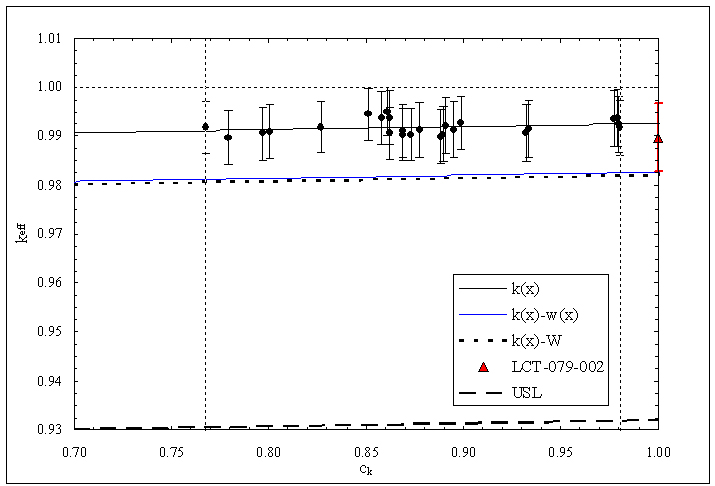
\includegraphics[keepaspectratio, width = 5 in]{images/trend_ck1}
    \caption{Example trending analysis using $c_k$ (for LCT-079-002).}
    \label{fig:trend_ck1}
\end{figure}


\begin{figure}[htp] 
    \centering
    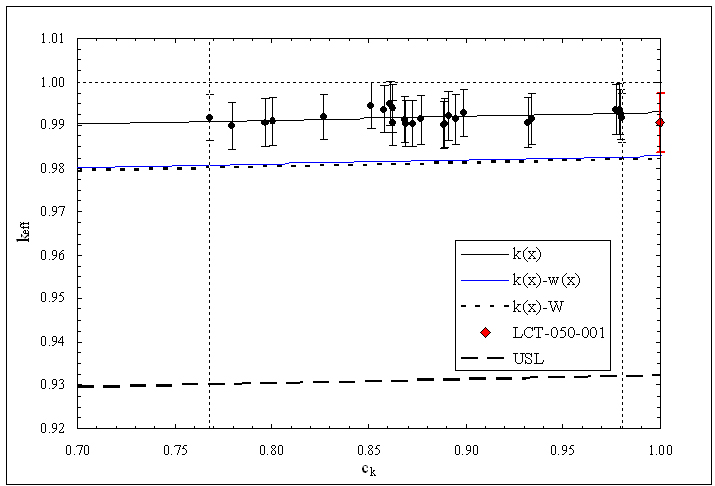
\includegraphics[keepaspectratio, width = 5 in]{images/trend_ck2}
    \caption{Example trending analysis using $c_k$ (for LCT-050-001).}
    \label{fig:trend_ck2}
\end{figure}

From the trends, the bias $k(x)-1$ (where $x$ is the parameter value 
for the application) and associated bias uncertainty (\ie $W$ from 
Eq. \ref{eq:confwidth}) can be computed in addition to the USL.  
Since the ``applications'' are known critical experiments, it is useful 
to compare the observed bias (\ie $k_{\mathrm{calc}} -1$) to the bias 
as predicted via trending.  Table \ref{tbl:trendbias} provides the 
observed and predicted biases (with uncertainty) and the USL for both 
applications.  For each application, all three methods yield very similar 
USL's, and all the biases are slightly underpredicted but well within 
one standard deviation of the observed biases.  

With such a large $\Delta k_m$, it is easy to wonder why we care 
about $\Delta \beta$. However, if we interpret subtracting $\Delta k_m$ 
from \keff as simply shifting the definition of critical, then it 
becomes clearer that $\Delta \beta$ is still important.

{\tiny
\begin{table}[hp]
 \caption{Observed and predicted biases ($\beta_{\mathrm{ob}}$ and 
         $\beta$), $\Delta \beta$, all in percent, and USL using 
         each trending technique.}
 \begin{center} 
 \begin{tabular*}{0.98\textwidth}{@{\extracolsep{\fill}} c|cccc|cccc } 
  \toprule
              & \multicolumn{4}{c}{LCT-079-002}          & \multicolumn{4}{c}{LCT-050-001} \\
   \midrule 
             & $\beta_{\mathrm{ob}}$ & $\beta$ & $\Delta \beta$  & USL & $\beta_{\mathrm{ob}}$& $\beta$  & $\Delta \beta$ & USL \\ 
   \midrule
       EALF  &  -1.08  &  -0.95  &  1.08  &  0.9298  &  -0.94  &  -0.77  &  1.08  &  0.9316 \\
    Enrich.  &  -1.08  &  -0.84  &  1.02  &  0.9314  &  -0.94  &  -0.85  &  1.02  &  0.9313 \\
      $c_k$  &  -1.08  &  -0.74  &  1.16  &  0.9306  &  -0.94  &  -0.71  &  1.07  &  0.9322 \\
  \bottomrule 
 \end{tabular*} 
 \end{center} 
 \label{tbl:trendbias}  
\end{table} 
}

\section*{Case Study: Burnup Credit}

\subsubsection*{Overview and Motivation}

The transportation and storage of used nuclear fuel is an integral component of any
nuclear fuel cycle. During handling of used nuclear fuel, strict attention must be paid
to criticality safety. The chief concern of criticality safety is to ensure the effective
multiplication factor \keff of the system in question is below unity at all times, i.e. to
ensure subcriticality.
For the case of used nuclear fuel, several factors affect the subcritical margin, i.e.
by how much a system is subcritical. Typical, unirradiated light water reactor (LWR)
fuel consists of uranium-oxide (UO2 ) enriched to 3-5\% ${}^{235}$U. During its time in the
reactor, nuclear fuel undergoes significant compositional changes, a process referred
to as burnup. Most importantly, the fissile isotope 235 U is depleted, generating various
fission products (FP's), many of which are parasitic neutron absorbers. Simultaneously,
${}^{235}$U breeds ${}^{239}$Pu which also undergoes fission and produces FP's. The net
effect of these compositional changes is to decrease the \keff of the fuel with increased
burnup. Accounting for this decrease in \keff (or equivalently, a decrease in reactivity)
in subcritical margins is often referred to as \textit{burnup credit}.

Historically, the so-called \textit{fresh fuel assumption} was used as a conservative bound
in criticality safety analysis of used nuclear fuel [1]. More recently, the Nuclear
Regulatory Commission (NRC) offered guidance for crediting the major (fissile) actinides
in such analyses in its Interim Staff Guidance - 8, revision 2 (ISG-8R2) report [2]. However,
even this results in a very conservative estimate of the subcritical margin of used
nuclear fuel.

Changes in the major actinides account for about 66-75\% of the net reduction
in reactivity; FP's account for the remainder, the percentages depending on burnup.
The FP's relevant to burnup credit, roughly in order of importance, include SM.
 
Why do we care?  Naturally, assuming a canister of some number of burned assemblies 
contains only fresh fuel is quite conservative.  Figure \ref{fig:loading_curve} shows 
loading curves for a generic used fuel canister with 32 WH 17x17 assemblies of varying 
initial enrichments and burnups.  Configurations below a given line do not meet subcritical 
limits under the given assumptions.  The reference case assumes fresh fuel, and each 
subsequence curve relaxes the assumptions.  

Considering that much of the current U.S. inventory of used fuel lies below the reference 
curve, a 32-assembly canister could not be widely used (and instead, canisters such as
the 21-assembly Transportation, Aging, and Disposal (TAD) canister intended for ultimate
disposition in Yucca Mountain would be required).  The cost of producing, loading, shipping, 
and disposing canisters is not negligible, and a study by Parks and Wagner suggest that
crediting the FP's in criticality safety analysis, thus allowing the high capacity
canisters, would potentially save upwards of \$200 million dollars in total disposal
costs \cite{parks2004csp}. 

\begin{figure}[ht] 
    \centering
    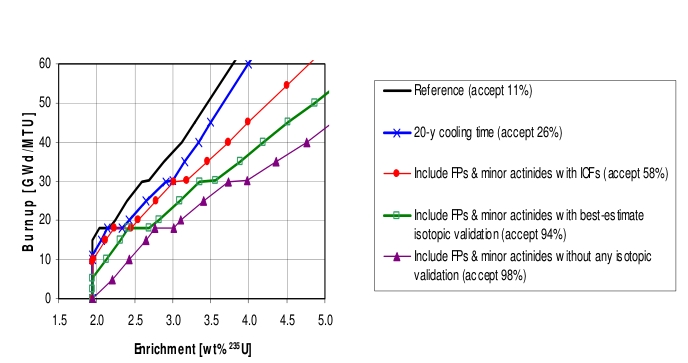
\includegraphics[keepaspectratio, width = 5.0 in]{images/loading_curve}
    \caption{Effect of calculational assumptions on loading curves for the GBC-32 and WH 17x17 assemblies.}
    \label{fig:loading_curve}
\end{figure}

\subsubsection*{Current Research}

To take into account the reduction in reactivity due to fission products,
called \textit{full burnup credit}, requires adequate knowledge of the 
isotopic content of the spent fuel (via validated depletion methods), and, 
our focus here, \textit{methods} to determine criticality and 
\textit{experiments} to validate those methods.

Current work has expanded on the S/U-based techniques
outlined above to develop methods for determinining biases of 
individual nuclides. While the details are beyond our scope, we give 
a brief description and several references for interested readers.

The basis of the work is the generalized linear least-square method (GLLSM).
GLLSM takes as input a set of nuclear data and covariances, the sensitivities 
of experiment models to nuclear data, the model \keff and uncertainty,
the experiment \keff and uncertainty (and any experiment correlation), 
and \textit{adjusts the nuclear data}
so that the the experiment and model \keff match.  It does so in a way that
minimizes the variation of all parameters (data and \keff) in terms of the
standard deviations of those parameters.  In other words, for all parameters
$p$, the method forces the experiment and model \keff to match while 
minimizing $\sum_i (\Delta p_i / \sigma_{p_i})^2$.  The adjustments can be 
propogated to an application's \keff via its model sensitivities, and the 
resulting difference is the bias.

To find biases of individual nuclides, the GLLSM method can be applied to 
so-called ``replacement experiments''.  These experiments consists of a single
reference case, and one or more cases that introduce some small perturbation
to the system, such as small foils of a fission product between fuel pellets 
\cite{buccx} or small concentrations of a fission product in a bulk
moderator \cite{french}.  GLLSM can then be applied to the reactivity 
difference between a reference-perturbation pair of models and experiements 
(rather than on the eigenvalue), since the sensitivities of the 
reactivity difference should be small for all but the perturbation 
material.  Consequently, the corresponding adjustment to the data should 
primarily be due to the test material, and as above, the adjustment can 
be propogated to the application to define a nuclide-specific bias.

\subsubsection{Limitations}

Two significant limitations apply to the methods under development.  First,
the methods require that relevant experiments are available.  However,
only a handful of experiments have been performed relevant to burnup credit,
and of those, the difference between reference and perturbation cases may 
be too high to extract partial biases.  Moreover, little data is available
for the correlation between experiments.  For the the reactivity difference
method described above, the resulting biases are extremely sensitive to 
the correlation between experiments. This suggests that future 
experiments should be designed with the various S/U methods as guidance.

A second, perhaps more significant issue is the general lack of reliable
nuclear covariance data.  Only for the most important isotopes does credible
data exist (such as uranium isotopes).  For isotopes of generally less
importance (like many fission products), little if any covariance data
exists.  Until reliable covariance data exists, the methods described
above are of limited value.
 
\section{Further Reading}

Much of the content in this lecture was inspired by Knief's 
\textit{Nuclear Criticality Safety: Theory and Practice} \cite{knief}.  Of
course, in one lecture, all that material cannot be covered, and the student
is directed to that book for more info most of the topics addressed here.
A more succinct overview of some of the topics is given by 
Peavey
in the \textit{Handbook of Nuclear Engineering} \cite{handbook}.  

For an overview of the application of sensitivity and uncertainty analysis
to criticality safety, see Broadhead et. al \cite{broadhead2004sau}, and
for the latest work on adjustment techniques applicable to full burnup
credit, see Rearden et al. \cite{reardenNT}.
%\include{equivalence_theory}
%\include{krylov_methods}
%\chapter{Numerical Diffusion}
\label{lec:numerical_diffusion}

In \LECTURE{pn_method_and_diffusion}, the diffusion approximation 
was formally derived.  In this lecture,  we present an approach 
for solving the diffusion equations numerically.  Diffusion theory 
represents an important method by itself.  Moreover, it finds widespread
use in the acceleration of higher-order transport methods, including 
the nonlinear diffusion acceleration of \LECTURE{nonlinear_acceleration} and
the linear preconditioners of \LECTURE{linear_acceleration}.

\section*{Mesh-Centered Diffusion Approximation}

The diffusion approximation can also be coupled with the 
multigroup treatment in multiple spatial dimensions.  Here,
we limit the discussion to the multidimensional, one-group
diffusion equation.  A full multigroup treatment is left as 
an exercise.

Consider the one-group diffusion equation
\begin{equation}
  -\nabla D(\vec{r}) \nabla \phi(\vec{r}) + \Sigma_r(\vec{r})\phi(\vec{r})
    = S(\vec{r}) \, ,
\label{eq:1gdiff}
\end{equation}
where $\Sigma_r$ is the ``removal'' cross section.  In the one-group
approximation, $\Sigma_r = \Sigma_a$.
To solve \EQ{eq:1gdiff} numerically, we use 
a mesh-centered, finite-volume approach, 
in which cell materials and sources are taken to be 
constant \cite{hebert2009arp}. 
By integrating \EQ{eq:1gdiff} over the volume $V_{ijk}$, one obtains
\begin{equation}
\begin{split}
 \int^{x_{i+1/2}}_{x_{i-1/2}} dx 
   \int^{y_{j+1/2}}_{y_{j-1/2}} dy 
     & \int^{z_{k+1/2}}_{z_{k-1/2}} dz 
    \Bigg \{ -\nabla D(\vec{r}) \nabla \phi(\vec{r})  
              + \Sigma_r(x,y,z) \phi(x,y,z) \Bigg \} \\
       &= \int^{x_{i+1/2}}_{x_{i-1/2}} dx 
            \int^{y_{j+1/2}}_{y_{j-1/2}} dy 
              \int^{z_{k+1/2}}_{z_{k-1/2}} dz \, S(x,y,z)  \, ,
\end{split}
\end{equation}
or
\begin{equation}
\begin{split}
 -D_{ijk} \Bigg [ \Delta_{y_j}  \Delta_{z_k} 
                   \Big (\phi_x(x_{i+1/2},y_j,z_k) &- \phi_x(x_{i-1/2},y_j,z_k) \Big ) \\
                 + \Delta_{x_i} \Delta_{z_k} 
                   \Big (\phi_y(x_i,y_{j+1/2},z_k) &- \phi_y(x_i,y_{j-1/2},z_k) \Big ) \\
                 + \Delta_{x_i}  \Delta_{y_j} 
                   \Big (\phi_z(x_i, y_j, z_{k+1/2}) &- \phi_z(x_i, y_j, z_{k-1/2}) \Big ) 
          \Bigg ] \\
     + \Delta_{x_i} \Delta_{y_j} \Delta_{z_k}  \Sigma_{r,ijk} \phi_{ijk} 
      &= \Delta_{x_i} \Delta_{y_j} \Delta_{z_k} S_{ijz} \, ,
\end{split}
\label{eq:integrateddiffeq}
\end{equation}
where the cell-centered flux (equal to the average flux) is defined as
\begin{equation}
 \phi_{ijk} \equiv 
   \frac{1}{\Delta_{x_i}}\frac{1}{\Delta_{y_j}}\frac{1}{\Delta_{z_k}} 
     \int^{x_{i+1/2}}_{x_{i-1/2}} dx 
     \int^{y_{j+1/2}}_{y_{j-1/2}} dy 
     \int^{z_{k+1/2}}_{z_{k-1/2}} dz \, \phi(x,y,z) \, ,
\end{equation}
the cell-average source is
\begin{equation}
 S_{ijk} \equiv 
   \frac{1}{\Delta_{x_i}}\frac{1}{\Delta_{y_j}}\frac{1}{\Delta_{z_k}} 
     \int^{x_{i+1/2}}_{x_{i-1/2}} dx 
     \int^{y_{j+1/2}}_{y_{j-1/2}} dy 
     \int^{z_{k+1/2}}_{z_{k-1/2}} dz \, S(x,y,z) \, ,
\end{equation}
and, for example, $\phi_x(x_{i+1/2},y_j,z_k)$ is the derivative of $\phi$ with 
respect to $x$, averaged over $y$ and $z$, and evaluated at $x=x_{i+1/2}$.

To evaluate the partial derivatives $\phi_x$, $\phi_y$, and $\phi_z$ in 
\EQ{eq:integrateddiffeq}, Taylor-series expansions are 
employed. For the
$x$-directed terms at the left (or west) boundary, let
\begin{equation}
  \phi(x_{i-1},y_j,z_k)  \approx 
      \phi(x_{i-1/2},y_j,z_k) - 
      \frac{\Delta x_{i-1}}{2} \phi^+_x (x_{i-1/2},y_j,z_k) 
 \label{eq:leftXexpA} 
\end{equation}
and
\begin{equation}
  \phi(x_{i},y_j,z_k)    \approx 
      \phi(x_{i-1/2},y_j,z_k) + 
      \frac{\Delta x_{i}}{2} \phi^-_x (x_{i-1/2},y_j,z_k) \, ,
 \label{eq:leftXexpB}
\end{equation}
with similar expressions for the right $x$ boundary and the 
$y$- and $z$-directed terms.  The $+$ and $-$ superscripts
on the partial derivatives indicate forward and backward extrapolation
from the cell midpoint,
respectively.
By continuity of net current, we must have
\begin{equation}
   D_{i-1,jk}\phi^+_x(x_{i-1/2},y_j,z_k) 
     = D_{ijz}\phi^-_x(x_{i-1/2},y_j,z_k) \, .
 \label{eq:contcurr}
\end{equation}
Multiplication of \EQ{eq:leftXexpA} by 
$D_{i-1,jk}/\Delta x_{i-1}$ and
\EQ{eq:leftXexpB} by $D_{ijk}/\Delta x_{i}$,
adding the results, and rearranging leads to
\begin{equation}
 \phi_{i-1/2,jk} = 
   \frac{D_{i-1,jk} \phi_{i-1,jk} \Delta_{x_i} + 
             D_{ijk} \phi_{ijk} \Delta x_{i-1}}
        {D_{i-1,jk} \Delta_{x_i} + D_{ijk} \Delta x_{i-1}} \, .
\end{equation}
Substituting this into the \EQ{eq:leftXexpB} gives
\begin{equation}
\begin{split}
 \phi_x(x_{i-1/2},y_j,z_k) &= 
  \frac{2}{\Delta_{x_i}} 
    \Bigg (\phi_{ijk} - 
           \frac{D_{i-1,jk} \phi_{i-1,jk} \Delta_{x_i} + 
                     D_{ijk} \phi_{ijk} \Delta x_{i-1}}
                {D_{i-1,jk} \Delta_{x_i} + D_{ijk} \Delta x_{i-1}} 
    \Bigg ) \\
  &= \frac{2}{\Delta_{x_i}} 
     \Bigg ( \frac{D_{i-1,jk} \phi_{ijk} \Delta_{x_i} + 
                       D_{ijk} \phi_{i-1,j,k} \Delta x_{i-1}}
                  {D_{i-1,jk}  \Delta_{x_i} + 
                       D_{ijk} \Delta x_{i-1}} \Bigg ) \\  
\end{split}
\end{equation}
or
\begin{equation}
  \phi_x(x_{i-1/2},y_j,z_k) = 
    2D_{i-1,jk} \Bigg ( \frac{\phi_{ijk} - \phi_{i-1,jk}} 
                             {\Delta_{x_i} D_{i-1,jk} + 
                              \Delta x_{i-1} D_{ijk}} 
                \Bigg ) \, ,  
\label{eq:phideriv1}
\end{equation}
Similarly, one finds
\begin{equation}
  \phi_x(x_{i+1/2},y_j,z_k) = 
    2D_{i+1,jk} \Bigg ( \frac{\phi_{i+1,jk}-\phi_{ijk}} 
                             {\Delta_{x_i} D_{i+1,jk} + 
                              \Delta x_{i+1} D_{ijk}} 
                \Bigg ) \,  .
\label{eq:phideriv2}
\end{equation}
These equations and the equivalents for $y$ and $z$ 
are substituted into
\EQ{eq:integrateddiffeq} to obtain a set of \emph{internal equations}.


\subsubsection{Internal Equation}
Substitution of Eqs.~(\ref{eq:phideriv1})~and~(\ref{eq:phideriv2})
into  \EQ{eq:integrateddiffeq} leads to
\begin{equation}
\begin{split}
  -D_{ijk} 
   \Bigg \{  
    \Delta_{y_j} \Delta z_j 
    \Bigg [ 
       2D_{i+1,jk} \Bigg (& 
                  \frac{ \phi_{i+1,j}-\phi_{i,j} } 
                       { \Delta_{x_i} D_{i+1,jk} + \Delta x_{i+1} D_{ijk} } 
                  \Bigg ) +  \\
       2D_{i-1,jk} \Bigg (& 
                  \frac{\phi_{i-1,j} - \phi_{i,j}} 
                       { \Delta_{x_i} D_{i-1,jk} + \Delta x_{i-1} D_{ijk} } 
                 \Bigg ) 
    \Bigg ] \ldots + 
   \Bigg \} + \\
   & \Delta_{x_i} \Delta_{y_j} \Delta_{z_k} \Sigma_{r,ijk} \phi_{ijk} 
   = \Delta_{x_i} \Delta_{y_j} \Delta_{z_k} S_{ijk} \, .
\end{split}
\label{eq:inteqs}
\end{equation}  
\EQUATION{eq:inteqs} represents the balance of neutrons in the
cell $(i,j,k)$.

We can further simplify the notation.  Let us define a coupling coefficient
\begin{equation}
 \tilde{D}_{i+1/2,jk} \equiv 
   \frac{2D_{i+1,jk}D_{ijk}}
        {\Delta_{x_i} D_{i+1,jk} + \Delta_{x_{i+1}} D_{ijk} } \, ,
\end{equation}
with similar coefficients for each direction.  Then 
we can rewrite Eq. \ref{eq:inteqs} as
\begin{equation}
 \begin{split}
     \frac{ \tilde{D}_{i+1/2,j,k}}{\Delta_{x_i}} 
         \Big (\phi_{ijk} - \phi_{i+1,j,k}  \Big ) 
  & +\frac{ \tilde{D}_{i-1/2,j,k}}{\Delta_{x_i}} 
         \Big (\phi_{ijk} - \phi_{i-1,j,k}  \Big ) \\
    +\frac{ \tilde{D}_{i,j+1/2,k}}{\Delta_{y_j}} 
         \Big (\phi_{ijk} - \phi_{i,j+1,k} \Big ) 
  & +\frac{ \tilde{D}_{i,j-1/2,k}}{\Delta_{y_j}} 
         \Big (\phi_{ijk} - \phi_{i,j-1,k} \Big ) \\
    +\frac{ \tilde{D}_{i,j,k+1/2}}{\Delta_{z_k}} 
         \Big (\phi_{ijk} - \phi_{i,j,k+1} \Big ) 
  & +\frac{ \tilde{D}_{i,j,k-1/2}}{\Delta_{z_k}}
         \Big (\phi_{ijk} - \phi_{i,j,k-1} \Big ) \\
  & + \Sigma_{r,ijk} \phi_{ijk} =  S_{ijk} \, .
 \end{split}
 \label{eq:inteqssimp}
\end{equation}
Note that each term on the left with a coupling coefficient represents
the net leakage from a surface divided by the area of that surface.

\subsubsection{Boundary Equations}

At the boundaries, we employ the albedo condition \cite{hebert2009arp}
\begin{equation}
 \frac{1}{2} D(x,y,z) \nabla \phi(x,y,z) \cdot \hat{n}(x,y,z) + 
 \frac{1}{4} \frac{1-\alpha(x,y,z)}{1+\alpha(x,y,z)}\phi(x,y,z) = 0 \, ,
\label{eq:albedo}
\end{equation}
where $\hat{n}$ is the outward normal, $\alpha$ describes the albedo 
condition ($\alpha = 0$ for vacuum, and $\alpha = 1$
for reflection).  

In three dimensions, a mesh cell has six surfaces, some of which 
may be part of a global surface.  As an example,
we consider the west global boundary:
\begin{equation}
 \text{west boundary}:  \,\,\,  
    -\frac{1}{2}D_{1jk} \phi_x(x_{1/2},y_j,z_k) + 
   \frac{1}{4}\frac{1-\alpha}{1+\alpha}\phi_{1/2,jk} = 0 \, .
\end{equation}
Because this expression contains $\phi$ at the edge, we again need to 
employ Taylor expansions.  For the west boundary, note that
\begin{equation}
 \phi_{1jk} \approx \phi_{1/2,jk} + \frac{\Delta_{x_i}}{2} \phi_x(x_{1/2},y_j,z_k) \, ,
\end{equation}
and we rearrange to get
\begin{equation}
 \phi_{1/2,jk} = \phi_{1jk} - \frac{\Delta_{x_i}}{2} \phi_x(x_{1/2},y_j,z_k) \, .
\end{equation}
Placing this into the albedo condition yields
\begin{equation}
\begin{split}
 0 =  -\frac{1}{2}D_{1jk} \phi_x(x_{1/2},y_j,z_k)  
  + \frac{1}{4}\frac{1-\alpha}{1+\alpha} 
    \Bigg ( \phi_{1jk} - \frac{\Delta_{x_i}}{2} \phi_x(x_{1/2},y_j,z_k) \Bigg ) \, ,
\end{split}
\end{equation}
and solving for $\phi_x(x_{1/2},y_j,z_k)$ gives
\begin{equation}
 \phi_x(x_{  1/2},y_j,z_k) = \frac{2(1-\alpha)\phi_{1jk}}
                                  {4(1+\alpha)D_{1jk} + \Delta_{x_1}(1-\alpha)} \, .
\end{equation}
For the east, we similarly find
\begin{equation}
 \phi_x(x_{I+1/2},y_j,z_k) =-\frac{2(1-\alpha)\phi_{Ijk} }
                                  {4(1+\alpha)D_{Ijk} + \Delta_{x_I}(1-\alpha)} \, ,
\end{equation}
and likewise for the other surfaces. Each of these  is placed into the proper 
partial derivative of \EQ{eq:integrateddiffeq}.  For example, the leakage
contribution on the left hand side of \EQ{eq:inteqssimp} due to leakage from 
the west boundary is transformed as 
follows\footnote{Ignore the fact that $\phi_{0jk}$ doesn't exist!}: 
\begin{equation}
  \frac{ \tilde{D}_{1/2,jk}}{\Delta_{x_1}}  \Big (\phi_{0jk} - \phi_{1jk}  \Big )  \rightarrow 
     \frac{2D_{1jk}(1-\alpha) \phi_{1jk}}
      {(4(1+\alpha)D_{1jk} + \Delta_{x_1}(1-\alpha))\Delta_{x_1}} \, .
\label{eq:west_leakage}      
\end{equation}


\subsubsection{Constructing the Diffusion Matrix}

The equations for cell balance derived heretofore can be combined into 
a linear system for the cell fluxes.  Generically, we can express this 
system as
\begin{equation}
 \mathbf{L}\vec{\phi} = \vec{S} \, ,
\end{equation}
where $\mathbf{L}$ is the  diffusion loss matrix. 
A straightforward implementation of the one-group diffusion loss matrix 
is presented in Listing~\ref{list:lossmatrix}.  Note that several 
parameters and helper functions require definition.  Although the 
code is set up for three dimensions, it can also be used for 1-D 
and 2-D problems by proper selection of boundary conditions.

\lstset{language=Python,caption=Sample code for construction of one-group loss matrix., label=list:lossmatrix, morecomment=[l]{\%}}
\begin{lstlisting}
L   = zeros((N, N))             # N x N loss matrix
remdims = [[1,2], [0,2], [0,1]] # For a given dim, provides remaining dims
# Loop over all cells
for n in range(0, N) :
  ijk = cell_to_ijk(n)          # Convert cardinal index to (i, j, k)
  w = [dx[ijk[0]], dy[ijk[1]], dz[ijk[2]]]
  # Loop over dimensions
  for dim in range(0, 3) :
    bound = [0, Nxyz[dim]]      # Minimum and maximum cell index in this dim
    # Loop over directions, + and -
    for dir in range(0, 2) :
      if ijk[dim] == bound[dir] :
        # Global boundary
        side = 3*dim + dir      # index of this side (0-5)
        B = beta[side]          # albedo for this side
        L[n][n] = L[n][n] + 2*D[n]*(1-B)/((4*(1+B)*D[n]+w[dir]*(1-B))*w[dir])
      else :
        # Coupling to neighbor at cell m
        ijk_m = ijk
        ijk_m[dim] = ijk_m[dim] + (-1)**dir
        m = cell_from_ijk(ijk_m)
        w_m = [dx[ijk_m[0]], dy[ijk_m[1]], dz[ijk_m[2]]]
        D_tilde = 2*D[n]*D[m]/((w[dir]*D[m]+w_m[dir]*D[n])*w[dir])
        L[n][m] = -D_tilde / w[dir]
        L[n][n] = L[n][n] + D_tilde / w[dir]
  # Add the removal cross-section component
  L[n][n] = L[n][n] + Sigma_r[n]
\end{lstlisting}


\begin{exercises}
 \item \textbf{Boundary Source}.  Suppose a partial current 
   $J^{\mathrm{west}-}_{jk}$ were incident on the west boundary 
   of cell $(1, j, k)$.  Show that the corresponding current 
   balance contribution (i.e., \EQ{eq:west_leakage}) is unchanged 
   but that the following source term arises:
  \begin{equation}
  Q^{\mathrm{boundary}}_{1jk} = \frac{8 D_{1jk} (1+\alpha) J^{\mathrm{west}-}_{jk}}
                                    {(4(1+\alpha)D_{1jk} + \Delta_{x_1}(1-\alpha))\Delta_{x_1}} 
  \end{equation}
 
  \item \textbf{One-Group Diffusion}.  For $\Sigma_t = 1.0$ and 
  $\Sigma_s = 0.0$, compute the flux.
  
  \item \textbf{Multigroup Diffusion}. 
    Although a formal derivation of the multigroup diffusion approximation
    requires assumptions beyond the ones
    made in \LECTURE{pn_method_and_diffusion},
    the resulting set of multigroup diffusion equations is intuitive:
    \begin{equation}
    \begin{split}
      -\nabla D_g(\vec{r}) \nabla \phi_g(\vec{r}) &+ 
        \Sigma_{rg}(\vec{r})  \psi_g(\vec{r})  = 
        \sum_{\substack{g'=1 \\ g'\neq g}}^{G} 
          \Sigma_{sg \gets g'}(\vec{r}) \phi_{g'}(\vec{r})  \\
        &+  \frac{\chi_g(\vec{r})}{ k}  
              \sum_{g'=1}^{G} 
                \nu\Sigma_{fg'}(\vec{r}) 
                  \phi_{g'}(\vec{r})
        +  S_g(\vec{r})  \, .
    \end{split}
    \label{eq:multigroupneutrondiffusionequation}
    \end{equation}
    Extend the routine proposed in Listing~\ref{list:lossmatrix} to handle 
    multigroup problems.
  
  
\end{exercises}

%\chapter{Linear Acceleration}
\label{lec:linear_acceleration}


While Krylov methods are generally more robust than the classical 
stationary methods, their performance can be improved significantly
via \emph{ preconditioning}.  A preconditioner $\oper{M}$ is an operator 
whose inverse satisfies $\oper{M}^{-1} \approx \oper{A}^{-1}$ in some sense 
and is relatively inexpensive to apply.

A \emph{ left preconditioned} linear system is
\begin{equation}
  \oper{M}^{-1}\oper{A}x = \oper{M}^{-1}b
\end{equation}
while a \emph{ right preconditioned} system is 
\begin{equation}
  \oper{A}\oper{M}^{-1} y = b
\end{equation}
with $x = \oper{M}^{-1} y$.  The left preconditioned residual differs 
from the original residual but may be a better metric for convergence. 
The right preconditioned system preserves the original residual.  

A preconditioner typically leads to a clustering of eigenvalues.  As 
an extreme example, suppose that $\oper{M} = \oper{A}$.  The 
preconditioned operator is then $\oper{AM}^{-1} = \oper{I}$, for 
which all the eigenvalues are unity.  Of course, to apply $\oper{M}^{-1}$ 
in this case represents solving the original problem.  While preconditioners
cannot in general be expected to yield a set of eigenvalues equal to unity, 
any clustering typically improves convergence.  Often, even pushing 
eigenvalues away from the origin tends to improve 
convergence \cite{larsen2010ado}.
Chapter \ref{chp:transport_pc} provides a relatively thorough 
development of several diffusion-based preconditioners for the 
transport equation.



Chapter \ref{chp:transport_methods} provided a short survey of trends in 
transport discretizations and solvers applicable to the fixed source 
multiplying problems relevant to response matrix methods.  As noted, 
Krylov methods have quickly become important tools for a variety of 
transport problems, but to be successful, they require adequate 
\emph{ preconditioning}.  
This chapter details several preconditioners 
relevant to transport calculations for reactor physics, and specifically 
the comparatively small problems characteristics of response matrix 
methods.

\index{preconditioner}

\section{Diffusion Synthetic Acceleration}
\index{DSA|see{diffusion synthetic acceleration}}
\index{diffusion synthetic acceleration}

Frequently, the most successful preconditioners are those that are based 
on \emph{ a priori} knowledge of the physics or structure of the problem.
This has long been the case for accelerating transport problems, for 
which early techniques enforced balance over coarse regions in space, 
angle, and energy.  

A related idea that has remained an important 
innovation is to apply a simple, low order approximation, invariably
based on diffusion, to provide an efficient update or correction to 
an unconverged transport solution.  Here, we provide a brief sketch 
of one diffusion-based scheme known as \emph{ diffusion synthetic 
acceleration} that has long been used but only recently as a 
preconditioner.  For simplicity, the development is given for the 
one group case, following the excellent treatment 
of Larsen and Morel \cite{larsen2010ado}.

Suppose we perform one source iteration, so that
\begin{equation}
  \phi^{n+\frac{1}{2}} = \oper{TMS} \phi^{n} + \oper{T}q \, .
\end{equation}
where $\oper{S}$ is assumed to contain both the 
scatter and fission within-group terms.
 Note the half index.  We subtract this equation 
from Eq. \ref{eq:wgteop} to get
\begin{equation}
 (\oper{I} - \oper{T}\oper{MS})\phi- \phi^{n+\frac{1}{2}} = 
   -\oper{TMS} \phi^{n} \, ,
\end{equation}
and adding $\oper{TMS} \phi^{n+\frac{1}{2}}$ to both 
sides and rearranging, 
\begin{equation}
 \epsilon = \overbrace{ ( \oper{I} - \oper{TMS})^{-1}\oper{T M} }^
                      {\text{what we approximate}}
            \overbrace{\oper{S} (\phi^{n+\frac{1}{2}}- \phi^{n})}^{v}
\label{eq:erroreq}
\end{equation}
where $\epsilon$ is the error.  Note the error satisfies the 
transport equation
\begin{equation}
 (\hat{\Omega} \cdot \nabla  + \Sigma) \varepsilon - 
   \frac{\Sigma_s}{4\pi} \epsilon =  \frac{v}{4\pi} \, ,
\end{equation}
where
\begin{equation}
 \epsilon = \int_{4\pi} d\Omega \, \varepsilon \, .
\end{equation}
Solving the error equation is just as expensive as solving the 
original transport equation.  As an alternative, we can use the 
diffusion approximation.  In this case, we have
\begin{equation}
 (-\nabla \cdot D \nabla + \Sigma - \Sigma_s) \epsilon = v \, ,
\end{equation}
or in operator form,
\begin{equation}
  \epsilon = \oper{C}^{-1} v = 
    \oper{C}^{-1} \oper{S} (\phi^{n+\frac{1}{2}}- \phi^{n}) \, .
\end{equation}
This leads to the update
\begin{equation}
\begin{split}
 \phi \approx \phi^{n+1} 
   &= \phi^{n+\frac{1}{2}} + 
      \oper{C}^{-1} \oper{S} (\phi^{n+\frac{1}{2}}- \phi^{n}) \\
   &= (\oper{I} + \oper{C}^{-1} \oper{S}) \phi^{n+\frac{1}{2}} - 
        \oper{C}^{-1} \oper{S} \phi^{n} \\
   &= \Big (\oper{I} - (\oper{I} + \oper{C}^{-1} \oper{S}) 
        ( \oper{I} -\oper{TMS}  ) \Big ) \phi^{n} 
       +  (\oper{I} + \oper{C}^{-1} \oper{S})\oper{T}q \\
   &= (\oper{I} - \oper{P}_{\text{WG-DSA}}^{-1}\oper{A}) \phi^{n} + 
        \oper{P}^{-1}_{\text{WG-DSA}}  \oper{T}q \, ,
\end{split}
\end{equation}
which is the preconditioned source iteration (i.e. source iteration 
plus diffusion synthetic acceleration), and where
\begin{equation}
 \oper{P}^{-1}_{\text{WG-DSA}}
   = (\oper{I} + \oper{C}^{-1} \oper{S})
\end{equation}
is the within-group diffusion preconditioning process.  In standard 
left-preconditioner form, we have
\begin{equation}
  \oper{P}_{\text{WG-DSA}}^{-1}\oper{A}
   =  \oper{P}^{-1}_{\text{WG-DSA}} \oper{T} q \, .
\end{equation}
Previous work indicates diffusion preconditioning coupled with a 
Krylov solver is less restrictive with respect to discretization and more 
effective for realistic problems \cite{warsa2004kim}.

\section{Multigroup DSA}

It is natural to extend the diffusion preconditioner to multigroup 
problems, yielding the process
\begin{equation}
  \oper{P}^{-1}_{\text{MG-DSA}} \equiv 
    \oper{I} + \oper{C}^{-1} 
     \left(\oper{S} + \oper{X}\oper{F}^T\right) \, ,
\label{eq:mgdsa}
\end{equation}
where $\oper{C}$ is the multigroup diffusion operator 
defined block-wise as
\begin{equation}
 \oper{C}_{gg'} \equiv 
   \delta_{gg'} 
   \left( \nabla \cdot D_g(\vec{r}) \nabla + \Sigma_{tg}(\vec{r}) \right ) 
   - \Sigma_{sgg'}(\vec{r}) - \chi_g \nu\Sigma_{fg'}(\vec{r}) \, .
\end{equation}
An initial review of the literature yielded no application of
multigroup diffusion 
as a preconditioner for multigroup transport problems.  
Related work addressed 
acceleration of outer Gauss-Seidel upscatter iterations \cite{adams1993tga}
and fission iterations based on the rank one fission 
operator ($\oper{X}\oper{F}^{\transp}$) \cite{morel1994fsa}, 
but all using an equivalent one group formulation.  
In general, the full multigroup diffusion problem is itself expensive
for large problems (an issue addressed below), and this may explain why  
it has not been used extensively.  

\section{Coarse Mesh Diffusion Preconditioning}
\index{preconditioner!coarse mesh diffusion preconditioner}

Preconditioning the multigroup equations with diffusion can lead to 
very large diffusion operators, and for many problems, the cost of 
constructing and, more importantly, applying the preconditioner becomes
prohibitive.  As an alternative, we investigate the use of coarse mesh
diffusion preconditioners.  Coarse mesh diffusion operators have long been
central to acceleration techniques in reactor analysis, a chief 
example being the nonlinear diffusion acceleration scheme developed
by Smith \cite{smith1984nms} for nodal diffusion methods and later 
extended to transport methods \cite{smith2002fct}.  

While no results could be found in the literature describing use of 
coarse mesh diffusion as a preconditioner, more general coarse mesh 
schemes in space, angle, and energy have been of substantial recent 
interest, particularly for multigrid preconditioning.  
Multigrid methods, like DSA (itself a two-grid method in angle), use 
a coarse grid solution to improve a fine grid solution by way of 
restriction (essentially averaging) and prolongation (essentially
interpolation) operations.  The idea is that slowly-varying, 
slowly-converging error modes become highly oscillatory, quickly-converging 
modes on the coarse mesh. While a complete description of multigrid 
methods is outside the present scope, the following sections describe 
implementation of a two-grid diffusion preconditioner.  For a more 
complete overview of multigrid methods, the reader would be best 
served by one of the standard reviews 
available, \eg Ref. \cite{briggs2000amt}.  

\subsection{A Spatial Two-Grid Multigroup Diffusion Preconditioner}

In this work, we apply a two-grid spatial scheme to the diffusion 
preconditioner.  Recent 
work suggests that multigrid methods in the energy variable can work very 
well \cite{hamilton2011nsk, slaybaugh2013mep}.  While a slightly different 
context, nonlinear diffusion acceleration also typically uses a coarse 
energy mesh to great effect. However, our initial studies using a coarsened
energy variable within a diffusion preconditioner suggests that the 
simultaneous restriction of space, angle, and energy may have inherent 
difficulties.

The coarse mesh diffusion preconditioner is a natural extension 
to Eq. \ref{eq:mgdsa} and is defined as
\begin{equation}
   \oper{P}^{-1}_{\text{MG-DSA}} \equiv 
    \oper{I} + \bm{P}\oper{C}_H^{-1}\bm{R}
     \left(\oper{S} + \oper{X}\oper{F}^T\right) \, ,
\end{equation}
where $\bm{P}$ and $\bm{R}$ are the \emph{ prolongation} and 
\emph{ restriction} operators, respectively, and 
$\oper{C}_H$ is the diffusion operator defined on the coarse 
spatial mesh.  

\subsubsection{Coarse Mesh Operator Homogenization}

To define $\oper{C}_H$, cross sections must be \emph{ homogenized} over 
the fine  mesh.  The most physically-sound approach for producing averaged 
cross sections is to use flux-weighting in a manner that preserves reaction
rates.  While a variety of such homogenization techniques exist, we use 
a rather conventional homogenization scheme that is simple to apply  
in preconditioning.  For the particular case of group constant generation
via an assembly-level lattice physics solver, the results of the scheme are 
referred to as \emph{ assembly homogenized cross sections} \cite{smith1986aht}.

To illustrate, suppose we need the total cross section $\Sigma_t$ averaged 
over coarse mesh cell $j$.  Denoting the fine mesh flux in cell $i \in j$ to 
be $\phi_i$, we have
\begin{equation}
  \Sigma_{t,j} = \frac{ \sum_{i \in j} V_i \phi_i \Sigma_{t, i} }
                      { \sum_{i \in j} V_i \phi_i } \, , 
\end{equation}
where $V_i$ is the fine mesh cell volume. If we define the coarse mesh 
flux to be the volume average
\begin{equation}
 \phi_j = \frac{\sum_{i \in j} V_ i \phi_i} {V_j} \, ,
\end{equation}
where 
\begin{equation}
 V_j = \sum_{i \in j} V_i \, ,
\end{equation}
then the total interaction rate in coarse cell $j$ is
\begin{equation}
 \sum_{i \in j} V_i \Sigma_{t, i} \phi_i =  
    \Sigma_j  \sum_{i \in j} V_i \phi_i =
    V_j \phi_j \Sigma_{t, j} \, .
\end{equation}
Hence, the averaged quantities preserve the integrated reaction
rate associated with the given fine mesh flux.  All group constants,
including the diffusion coefficient $D$, can be generated in this way.

The obvious problem with this approach is that the fine mesh flux 
$\phi_i$ is not known. The simplest approximation is to assume a 
constant flux, leading to  volume-weighted cross sections.  For 
preconditioning,  this is a suitable approximation, since 
conserving true reaction rates is not a prerequisite.  Unlike 
certain nonlinear acceleration techniques (\eg CMFD) that rely on 
conservation to provide an integral form of the \emph{ solution} at 
each step, preconditioning---a linear process---only seeks to provide 
an additive improvement.

However, that certainly does \emph{ not} preclude use of more accurate 
flux shapes to achieve better results. 
In typical lattice physics applications, group constants are 
found by solving the transport equation in a pincell or assembly subject 
to reflecting conditions and using the resulting spectrum for weighting.  
For preconditioning, a simple pincell homogenization scheme could be used, 
in which 2-D pincell problems approximating parts of the full problem 
are solved, and the resulting region-wise volume-averaged spectra are used to 
produce homogenized materials in the appropriate cells.  Analysis of this 
approach would be a natural extension to the present work.

One might note that the current flux iterate is 
freely available for use in homogenization; however, because the flux 
and homogenization process would change from step to step, the entire 
process would become nonlinear, and its application within the context 
of standard Krylov linear solvers would be suspect.  Its use 
in solvers allowing variable preconditioners (\eg FGMRES \cite{saad1993fio})
would be valuable future research.

\subsubsection{Restriction}

To restrict the fine mesh input vector for application of the inverse coarse 
mesh diffusion operator, a simple spatial average is used.  As an example, 
consider a 1-D problem discretized into 6 fine meshes.  The coarse 
meshing process is based on a level parameter $l$ that defines the 
number of fine meshes per coarse mesh.  Suppose $l=2$, leading to 
the fine-to-coarse mapping $[0,0,1,1,2,2]$.  The restriction operator
is defined 
\begin{equation}
  \bm{R} = 
           \left(
           \begin{array}{cccccc}
              v_0 & v_1 &  0  &  0  &  0  &  0  \\
                0  &  0 & v_2 & v_3 &  0  &  0  \\
                0  &  0 &  0  &  0  & v_4 & v_5  \\
           \end{array} 
           \right ) \, ,
\end{equation}
where
\begin{equation}
 v_i = \frac{V_i}{V_j} \, , \quad \quad
   \text{for fine mesh $i$ in coarse mesh $j$} \, ,
\end{equation}
and hence $\sum_{i\in j} v_i = 1$.

\subsubsection{Prolongation}

To prolong the coarse mesh result back to the fine mesh, the coarse mesh 
value is distributed on the fine grid based on the (approximate) 
flux $\tilde{\phi}$ used to produce the coarse mesh diffusion operator.  
Given a coarse mesh value $\phi_j$, the prolonged flux is defined as 
\begin{equation}
 \phi_{i \in j} =   \phi_j   \frac{l\tilde{\phi}_i}
                                  {\sum_{i \in j} \tilde{\phi}_i} \, .
\end{equation}
For the example above, suppose each coarse region is assumed to have 
a fine mesh flux shape of $\tilde{\phi} = [a, b]$, where $a + b = 1$.  The 
prolongation operator is defined 
\begin{equation}
  \bm{P} = 
           \left(
           \begin{array}{ccc}
                2 a  &  0      &  0     \\
                2 b  &  0      &  0     \\
                  0  &  2 a    &  0     \\
                  0  &  2 b    &  0     \\
                  0  &  0      &  2 a \\
                  0  &  0      &  2 b \\
           \end{array} 
           \right ) \, .
\end{equation}
In the constant flux approximation ($a = b = 0.5$), multiplication 
of $\bm{R} \in \mathbb{R}^{n\times m}$ by  
$\bm{P} \in \mathbb{R}^{m\times n}$ yields the identity matrix 
$\oper{I} \in \mathbb{R}^{n\times n}$.


\subsubsection{Smoothing}

While the coarse mesh scheme described so far represents a complete 
preconditioner, it can be significantly improved by a \emph{ smoothing} 
operation.  The motivation for smoothing is that the coarse mesh solve damps 
low frequency error modes of the fine 
mesh problem but not high frequency modes.  In more physical terms, a 
coarse mesh solve can be expected to get the gross shape right, but 
not the finer details.  A smoothing operator uses a few iterations of 
a classical scheme like Richardson, Jacobi, or Gauss-Seidel with the fine 
mesh operator.  In many multigrid algorithms, a smoother is also often 
used before the coarse mesh solve to ensure the error is ``smooth'' 
before restriction; however, in this case the joint scattering and 
fission operator $\oper{S}+\frac{1}{k} \oper{XF}^{\transp}$ precedes 
the coarse mesh solve and can be expected to provide a suitable input vector.

For the coarse mesh diffusion preconditioner, smoothing requires the action 
of the fine mesh diffusion matrix.  While the cost of producing this 
matrix may be somewhat large, that cost is much smaller than inverting 
the operator in a fine mesh preconditioner (and much, much smaller than
application of the transport operator).  The smoothing process used is 
the weighted Jacobi method, which for the generic problem $\oper{A}x=b$ is 
defined  by the process 
\begin{equation}
 x^{(n+1)} = -\omega \oper{A}_D^{-1} ( \oper{A}_L + \oper{A}_U) x^{(n)}
           + (1-\omega) \oper{A}_D^{-1} b \, ,
\end{equation}
where $\oper{A}_D$ represents the diagonal of $\oper{A}$, 
$\oper{A}_L$ and $\oper{A}_U$ represent the strictly lower and strictly 
upper triangular parts of $\oper{A}$, and $\omega$ is the weighting 
parameter.  For completely solving the linear system, $\omega = 1$ is ideal 
(with $\omega > 1$ potentially yielding instability);
however, for the purposes of damping high frequency errors, the optimum is 
typically smaller, with special 1-D and 2-D model cases having optima 
of $\omega = \frac{2}{3}$ and $\omega = \frac{4}{5}$, 
respectively \cite{saad2003ims}.  
Algorithm \ref{alg:cmdsa} provides a basic outline of the coarse mesh 
diffusion preconditioner.

\begin{algorithm}[ht]
  \SetCommentSty{small}
  \DontPrintSemicolon
  \KwData{Input vector $v_0$, 
          number of smoothing iterations $N$,
          weighting factor $\omega$}
  \KwResult{Preconditioned vector $v_1$}
  \tcp{Apply the scattering and fission operator}
  $x = (\oper{S} + \frac{1}{k}\oper{XF}^{\transp}) v_0$ \;
  \tcp{Apply restriction}
  $x_H = \oper{r}x$ \;
  \tcp{Solve the coarse mesh diffusion problem}
  $y_H = \oper{C}^{-1}_H x_H$ \;
  \tcp{Apply prolongation}
  $z = \oper{p} y_H$ \;
  \tcp{Optionally apply smoothing}
  \For{$i$ from 1 to $N$}
  {
    $z =  -\omega \oper{C}_D^{-1} ( \oper{C}_L + \oper{C}_U) z
       + (1-\omega) \oper{C}_D^{-1} x $
  }
  \tcp{Compute output vector}
  $v_1 = v_0 + z$\;
  %\tcp{If not converged, restart with $u$ and $\lambda$}
  \caption{Two-Grid Coarse Mesh Multigroup Diffusion Preconditioner}
  \label{alg:cmdsa}
\end{algorithm}

%---------------------------------------------------------------------------%
\section{Transport-Corrected Diffusion Preconditioners}
\label{sec:tcdpc}
\index{preconditioner!transport-corrected diffusion preconditioner}

\subsection{Explicit Versus Matrix-Free Transport Operators}

A final technique developed is to form a preconditioner that contains
information from the transport operator rather than relying solely on 
the diffusion approximation.   In theory, forming the transport operator 
defined by Eq. \ref{eq:mgto} explicitly is possible.
With an explicit operator, various 
approximate factorizations become natural preconditioner options. 
However, constructing such operators implies working with matrices with 
sizes proportional to the  number of angles, at least implicitly, as part 
of the construction process. This can quickly lead to huge memory 
requirements, a complicated  construction process, or both.  

Construction of explicit transport operators have been studied for 
for the discrete ordinates method \cite{patton2002apg} and for the method of 
characteristics \cite{zhang2011ctm}. The former work treated the angular 
flux directly, and the analysis was limited to relatively small multigroup
1-D problems.  The latter work noted the cost of constructing the 
transport operator was exceedingly large and developed a marginally 
successful parallel scheme limited to the within-group equations.

In the present work, the transport operator is always a 
``matrix free'' operator,  meaning that the action $y \gets \oper{A}x$
is done by functions and not explicit matrix operations.  Hence, while 
the action of $\oper{A}$ is available, $\oper{A}$ itself is not,  
so preconditioners based on approximate factorizations are not directly 
applicable.  Ultimately, we restrict any preconditioner using a 
transport operator to be based on actions only.

\subsection{Newton-based Correction}

As an alternative, suppose we have a matrix inverse 
$\oper{M}^{-1}$ that represents an initial approximation of 
$\oper{A}^{-1}  \in \mathbb{R}^{m\times m}$.  For application to 
transport problems, we let $\oper{M}$ be the diffusion 
preconditioner $\oper{P}_{\text{MG-DSA}}$ or its coarse mesh equivalent.
Our goal is to improve this preconditioning process using the 
(possibly approximate) action of $\oper{A}^{-1}$.

To do this, we apply a method attributed by various sources to 
Shulz or Hotelling and Bodewig \cite{schulz1933ibr, householder1975tmn}, 
but in fact which represents application of Newton's method for 
finding a matrix inverse.  For brevity, we refer to it as the 
Newton-Shulz method.  While a more rigorous analysis of the method 
can be found elsewhere \cite{householder1975tmn}, it is possible to
motivate it by considering the simple problem $ax=1$ 
following Ref. \cite{chow1998aip}.  Given
$a$, we seek $x$.  One way to view this is as the nonlinear 
problem $f(x) = 1/x-a = 0$.  Then $f'(x) = -1/x^2$, and Newton's 
method (see Section \ref{sec:newtonsmethod}) gives the process
\begin{equation}
\begin{split}
 x_{n} &= x_{n-1} + \frac{1}{x_{n-1}^{-2}} 
           \left( \frac{1}{x_{n-1}} - a \right) \\
       &= 2x_{n-1} - x_{n-1} a x_{n-1} \, .
\end{split}
\end{equation}
For the more general case of matrices, this suggests 
the process 
\begin{equation}
 \oper{X} = \oper{X}(2\oper{I} - \oper{A}\oper{X}) \, ,
\end{equation}
where $\oper{X} \approx \oper{A}^{-1}$.  

As is always the case for Newton's method, convergence 
to the solution depends on the initial guess being sufficiently close to 
the solution.  
% In practice, the guess $ \oper{X} = \alpha \oper{A}^T$ can 
% be shown to guarantee convergence.  
By using $\oper{P}_{\text{MG-DSA}}$ as 
the initial guess, convergence has always been achieved in our studies.
Hence, a simple one step transport-corrected diffusion preconditioning 
process is defined by
\begin{equation}
 \oper{P}_{\text{TC-MG-DSA-1}}^{-1} = 
   \oper{P}_{\text{MG-DSA}}^{-1}(2\oper{I} - 
             \oper{A}_{\text{MG}} \oper{P}_{\text{MG-DSA}}^{-1}) \, .
\label{eq:tc1mgdsa}
\end{equation}

While Eq. \ref{eq:tc1mgdsa} represents an improved preconditioner, 
it adds the cost of an additional space-angle-energy sweep, the number 
of which we are ultimately trying to minimize.  As an alternative, 
we can substitute 
\begin{equation}
 \oper{A}_{\text{MG}} \approx \oper{\tilde{A}}_{\text{MG}} \, ,
\end{equation}
where the tilde indicates some approximation.  Here, we let that 
imply a coarser angular quadrature.  While this appears at first to be a 
multigrid method, note that the (approximate) transport operator is 
not being inverted but rather is being used to improve the inversion of 
the diffusion preconditioner.  In the terminology of Newton methods, 
using the approximate operator results in an approximate Jacobian.

Because only a few iterations of Newton's method are needed to 
converge given an appropriate initial guess, using the approximate 
operator $\oper{\tilde{A}}_{\text{MG}}$ will lead to \emph{ its} approximate
inverse and \emph{ not} that of $\oper{{A}}_{\text{MG}}$.
However, $\oper{\tilde{A}}^{-1}_{\text{MG}}$ should be even 
closer to $ \oper{A}^{-1}_{\text{MG}}$ than the original diffusion 
preconditioning process, and so application of the full transport operator 
can be expected to yield a much more valuable improvement if used in one 
final Newton iteration.  

Algorithm \ref{alg:tcmgdsa} provides the 
complete preconditioning process for application to an input 
vector based on the recursive application of the Newton-Schulz method
defined in Algorithm \ref{alg:newtonshulz}.  
The true operator is only applied once in the last step, but the number of 
actions of $\oper{\tilde{A}}$ grows exponentially with the number 
of iterations: one for $k=2$, three for $k=3$, seven for $k=4$, and 
so on.  
Hence, the cost of applying the preconditioner is likely to 
become excessive for more than two or three iterations unless the 
approximate operator is significantly less expensive than the 
true operator.

\begin{algorithm}[ht]
  \SetCommentSty{small}
  \DontPrintSemicolon
  \KwData{transport operator $\oper{A}$,
          approximate transport operator $\oper{\tilde{A}}$,
          diffusion preconditioner $\oper{P}_{\text{MGDPC}}$,
          number of corrections $k$,
          input vector $x$}
  \KwResult{output vector $y$}
  $y \gets \text{Newton-Shulz}(\oper{\tilde{A}}, \oper{P}_0, k-1, x)$ \;
  $y \gets \oper{A}y$ \;
  $y \gets 2x - y$ \;
  $y \gets \oper{P}^{-1}_0 y$ \;
  \caption{Transport-Corrected Diffusion Preconditioner}
  \label{alg:tcmgdsa}
\end{algorithm}

\begin{algorithm}[ht]
  \SetCommentSty{small}
  \DontPrintSemicolon
  \KwData{operator $\oper{A}$, 
          initial preconditioner $\oper{P}_0$,
          number of corrections $k$,
          input vector $x$}
  \KwResult{output vector $y$}
  \uIf{$k > 1$}
  {
    \tcp{Apply earlier steps recursively}
    $y \gets \text{Newton-Shulz}(\oper{A}, \oper{P}_0, k - 1, x)$ \;
    $y \gets 2x- \oper{A}y$\;
    $y \gets \text{Newton-Shulz}(\oper{A}, \oper{P}_0, k - 1, y)$ \; 
  }
  \Else
  {
    \tcp{Apply the initial preconditioner}
    $y \gets (2\oper{I}-\oper{A} \oper{P}^{-1}_0) x$ \;
    $y \gets \oper{P}^{-1}_0 y$ \;
  }
  \caption{Newton-Shulz}
  \label{alg:newtonshulz}
\end{algorithm}

\section{Summary}

This chapter has presented the classic diffusion 
synthetic acceleration technique and its multigroup analog in the 
context of preconditioning for iterative transport solvers.  Additionally,
a coarse mesh variant was proposed based on two spatial grids and 
optional smoothing that represents in theory a 
much less computationally-intensive process than the fine mesh 
preconditioner. To incorporate more of the transport operator, 
the Newton-Shulz method was used to form a transport-corrected 
diffusion preconditioner that has the potential to yield better 
preconditioners than diffusion alone can provide.
%\include{advanced_sn_discretization}
%\chapter{Method of Characteristics}

%\chapter{Coupling Transport to Other Physics}

In \LECTURE{time_dependent_transport}, we developed numerical 
schemes for the solution of time-dependent problems.  In this 
lecture, we extend that development to include transient dependence
on other physics such that cross sections and other system 
coefficients depend, in some manner, on the particle flux.  We'll 
identify two basic approaches for the solving such coupled-physics 
problems and discuss the advantages and disadvantages of each.


%\include{homogenization}
%\include{analytic_multigroup}
%\include{nodal_diffusion}
% \chapter{Automated Variance Reduction}

In this lecture, automated variance reduction techniques 
for Monte Carlo shielding problems are investigated. 
Typically, these shielding problems 
are difficult because they represent massive attenuation of source 
particles, and, hence, require many histories to achieve adequate statistics.  
Variance reduction reduces the effort by modifying the underlying sampling 
scheme in an unbiased way so that  the same statistics are achieved with 
less computation.  The techniques investigated in this paper 
are ``automated'' in the sense that comparatively inexpensive deterministic 
solutions are used to generate parameters for use in both source and 
transport biasing schemes.  We demonstrate the efficacy of several 
algorithms for simple multigroup slab problems using a discrete ordinates 
solution to generate biasing parameters.

\section{Introduction}

The Monte Carlo method is widely believed to be the most accurate method 
for solving problems in radiation transport.  Unfortunately, due to its 
very nature---following individual particle histories---certain classes 
of problems are particularly challenging for the method.  One such class 
of problems consist of so-called deep penetration shielding problems.  
Because the purpose of a shield is to attenuate a particle population by 
several orders of magnitude, to use the Monte Carlo method requires a 
sufficient number of histories to ensure that the population, once attenuated, 
can still provide adequate statistics.  For deep penetration problems, the 
level of attenuation makes Monte Carlo prohibitively expensive.

To circumvent this issue, several approaches for \emph{variance reduction} have
been developed over the years.  Variance reduction techniques aim to modify (\ie
bias) in some manner the underlying physics in such a way that an \emph{unbiased}
solution with \emph{lower} statistical error is found than an unbiased simulation
using the same computational resources.  Haghighat and Wagner
\cite{haghighat2003mcv} classify variance reduction techniques in three ways:
\emph{modified sampling methods} (e.g., source biasing, implicit capture), 
\emph{population control methods} (e.g., geometry splitting/roulette, weight windows),
and 
\emph{semi-analytical methods} (e.g., point detectors and DXTRAN).  
In this lecture, we only analyze methods falling in the first two 
categories, i.e.,
approaches for source biasing, geometry splitting/roulette, and
weight windows.  Moreover, we see \emph{automated} approaches 
for these methods.  

The lecture is is organized as follows.  In Section \ref{sec:tech}, we
describe several approaches to variance reduction that use the adjoint or
forward fluxes computed via the discrete ordinates method to select parameters
for source biasing, geometry splitting, or weight windows. We apply those
techniques in Section \ref{sec:results} to some simple slab problems and
summarize the impact each technique has on various problem types. Section
\ref{sec:conc} provides several concluding remarks.  

\section{Automated Variance Reduction Techniques}
\label{sec:tech}

In this section, we describe several automated approaches for variance
reduction.  They are ``automated'' in the sense that essentially no user input
is required to generate parameters (\eg the user need not define cell
importances for geometry splitting).  Throughout, it is assumed that an
approximate forward and/or adjoint flux is available, \eg from a discrete
ordinates calculation.

\subsection{Geometry Splitting}

Geometry splitting and roulette is a common variance reduction technique that
can yield a substantial reduction in computational expense.  The essential idea
of geometry splitting is to encourage more particles (of less weight) to fill a
region of high importance.  On the other hand, the technique aims to reduce the
computational effort of tracking particles in unimportant regions.  Here, we
outline the basic algorithm for geometry splitting.

First, the importance of a cell is taken to be the adjoint flux
spatially-averaged over a cell.  Note, this implies that a cell importance may
still be energy-dependent.  When a particle of weight $w$  exits a cell $A$ with
importance $I_A$ and enters a cell $B$ with importance $I_B$ (with $I_A \neq
I_B$), two options exist: either $I_B > I_A$ or $I_B < I_A$.  In the first case,
the particle is split into a number of particles dependent on the ratio of the
importances.  In the latter case, the particle undergoes roulette and is either
eliminated or survives with increased weight. Algorithm \ref{alg:geom} provides
the basic implementation. 

\begin{algorithm}
 \label{alg:geom}
 \caption{Geometry Splitting and Roulette}
 $r \leftarrow$ $I_B/I_A$ \;
 \eIf{$r > 1$}{
   \eIf{ $\xi < r - \lfloor r \rfloor$}{
     $n$ $\leftarrow$ $\lceil r \rceil$ \;
   }{
     $n$ $\leftarrow$ $\lfloor r \rfloor$ \;
   }
   $w'$ $\leftarrow$ $w/r$ \;
   bank $n-1$ particles and keep following first \;
 }{
   \eIf{$\xi < r $}{
     $w'$ $\leftarrow$ $w/r$ \;
   }{
     kill particle \;
   }
 }
\end{algorithm}

It is worth noting that the algorithm above is  ``expected-value splitting''
which takes $ w' = w/r$ (\ie no rounding) and  chooses $n = \lfloor r \rfloor $
or $ n= \lceil r \rceil$ \cite{booth1985mcv}.  This is in contrast to ``sampled
splitting'' which chooses  $n = \lfloor r \rfloor$ or $ n = \lceil r \rceil$
(via sampling) and  defines the weight to be $w'=w/n$ \cite{booth1985mcv}.  
Sampled splitting has the benefit of conserving particle weight at each
individual split while the expected-value splitting does so only on average. 
However, because the sampled splitting approach introduces varying weights at a
particular geometry interface, it may adversely affect the variance (whereas the
latter approach does not) \cite{haghighat2003mcv}.  Note further that the
simplified sampled splitting method given by Brown \cite{brown2005fmc} does not
introduce weight fluctuations but does not capture the importance ratio exactly.

\subsection{CADIS}

The Consistent Adjoint-Driven Importance Sampling (CADIS) method was developed
by Wagner and Haghighat \cite{wagner1998avr}.  The key idea of CADIS is that the
transport biasing (via weight windows) and source biasing are derived in a
consistent manner from the adjoint function.  Here, we give an overview of the
use of the adjoint in source and transport biasing and how such biasing can be
translated into weight window parameters, largely following Wagner and Haghigat
\cite{wagner1998avr}.  Note, this development also forms the basic core of the
FW-CADIS and pseudo-Cooper methods described below.

\subsubsection{Source Biasing}

We define the response of interest to be
\begin{equation}
 R = \int_P \psi (P) \sigma_d(P)dP \, ,
\end{equation}
where $\psi$ is the forward angular flux, $\sigma_d$ is an objective function
(perhaps a flux-to-dose constant), and $P$ represents the spatial-, energy-, and
angular-dependent phase space.  Using the well-known adjoint identity
\begin{equation}
 \langle \psi^\dag H \psi \rangle = \langle \psi H^\dag \psi^\dag \rangle \, ,
\end{equation}
where $\psi^\dag$ is the adjoint angular flux, $H^\dag$ is the adjoint transport
operator, and  $\langle \rangle$ represents integration over all phase space, it
is possible to show that 
\begin{equation}
 R = \int_P \psi^\dag (P) q(P)dP \, ,
\end{equation}
where $q$ is a forward source density.  Hence, we find that $\psi^\dag$ can be
interpreted physically as the expected contribution of a particle anywhere in
phase space to the response of interest (\ie the particle importance).

We can use this notion of $\psi^\dag$ to bias the source density $q$ via
\begin{equation}
 \hat{q} = \frac{\psi^\dag(P) q(P) }{ \int_P \psi^\dag(P) q(P) dP } \, ,
 \label{eq:biassrc}
\end{equation}
which can be shown to minimize the variance for $R$.  The particle weights are
then defined to be
\begin{equation}
 w(P) = \frac{R}{\psi^\dag(P)} \, .
\end{equation}

\subsubsection{Transport Biasing}
 To investigate transport biasing, consider the integral form of the transport
equation,
\begin{equation}
 \psi(P) = \int f(P'\to P) \psi(P') dP' + q(P) \, ,
\end{equation}
where $f(P' \to P) dP$ is the expected number of particles entering $dP$ about
$P$ due to an interaction in $P'$, and $q(P)$ is the (forward) source density. 
We define
\begin{equation}
 \hat{\psi}(P) = \frac{ \psi^\dag(P)\psi(P) }{ \int \psi^\dag(P)\psi(P) dP } \,
,
 \label{eq:contflux}
\end{equation}
from which we find a transformed integral equation in terms of the biased
source:
{\footnotesize
\begin{equation}
\begin{split}
 \hat{\psi}(P) &= \int dP' f(P'\to P) \frac{ \psi(P')\psi^\dag(P) }{ \int
\psi^\dag(P)\psi(P) dP} + \hat{q}(P) \\
               &= \int dP' f(P'\to P) \frac{ \psi(P')\psi^\dag(P) }{ \int
\psi^\dag(P)\psi(P) dP}  \frac{ \hat{\psi}(P') \int \psi^\dag(P')\psi(P')
dP}{\psi^\dag(P')\psi(P') }+ \hat{q}(P) \\
               &= \int dP' f(P'\to P) \frac{ \psi^\dag(P) \hat{\psi}(P')
}{\psi^\dag(P') }+ \hat{q}(P) \, .
\end{split}
\label{eq:modeq}
\end{equation}
}
In more compact form, we have
\begin{equation}
  \hat{\psi}(P) = \int \hat{f}(P' \to P) \hat{\psi}(P') dP' + \hat{q}(P) \, ,
\end{equation}
where \footnote{It is interesting to note that the modified flux $\hat{\psi}$ in
Eq. \ref{eq:contflux} is just the normalized ``contributon flux'' and $\hat{f}$
of Eq. \ref{eq:modf} is akin to the ``contributon cross-section'' (see \eg the
interesting paper by M. Williams \cite{williams1991gcr}).  With these
interpretations, one can arrive (in hand-waving fashion) to the notion of zero
variance.  Since ''contributons'' represent exactly a flow of response from the
source to the detector, their very existence gives use what we want; of course,
that requires both a perfect knowledge of the adjoint and a way to use it
completely.  Unfortunately, we have neither.}
\begin{equation}
 \hat{f}(P' \to P) = f(P' \to P) \frac{\psi^\dag(P) }{\psi^\dag(P') } \, .
 \label{eq:modf}
\end{equation}
Here, $\hat{f}$ represents a biased transfer function that acts to bias the
transport process, and $\hat{\psi}$ is the corresponding solution (essentially a
contributon flux, a quantity with a very definite physical interpretation that
the authors never quite point out; see the note below).  

In general $f(P'\to P)$ is not known, so the modified transport Eqs.
\ref{eq:modeq} and \ref{eq:modf} cannot be solved.  However, Eq. \ref{eq:modf}
in particular suggests a possible way to modify the population of particles
propagating through phase space.  If a particle in phase space $P'$ enters a
region in phase space $P$ which is more (less) important than $P'$, then
particles can be split (rouletted) based on the value of $\psi^\dag (P) /
\psi^\dag (P')$.  This is exactly the idea used in geometry splitting above, but
for geometry splitting, the ratio of adjoints is determined only at cell
boundaries and not after every interaction in phase space.  After
splitting/rouletting, the particle weights are defined via
\begin{equation}
 w(P) = w(P') \frac{\psi^\dag(P')}{\psi^\dag(P)} \, .
\end{equation}

\subsubsection{Implementation}
To implement CADIS, we follow the approach of Wagner and Haghighat in their
implementation of CADIS in MCNP \cite{wagner1998avr}.  Because storing adjoint
information for all (discretized) phase space can be very expensive for large
problems, the angular variable is integrated out of all the quantities of the
previous sections.  Consequently, our biased source density becomes
\begin{equation}
 \hat{q}(r,E) = \frac{\phi^\dag(r,E) q(r,E) }{ \int_E \int_V \phi^\dag(r,E)
q(r,E) dr dE } \, ,
 \label{eq:biassrc2}
\end{equation}
where $\phi^\dag(r,E)$ is the adjoint scalar flux, and the particle weights are
defined as
\begin{equation}
 w(r,E) = \frac{R}{\phi^\dag(r,E)} \, .
\end{equation}

For transport biasing, the weight window approach is used.  The goal of
weight-windows is not only to encourage a large number of particles toward a
desired region of phase space but to ensure the particles have weights
distributed in a relatively narrow range.  A low variance in the weights of
particles reaching a detector corresponds directly to a detector response with
low variance.  Whenever a particle of weight $w$ enters a region of phase space
with a weight window defined by a lower weight $w_L$ and upper weight $w_U$,
three possibilities exist.  First, if $w$ is within the weight window, then
nothing occurs.  If instead $w < w_L$, a game of roulette is played.  Finally,
if $w > w_L$, then the particle is split. Algorithm \ref{alg:ww} outlines a
basic weight-window approach modified from \cite{brown2005fmc}.

\begin{algorithm}
 \label{alg:ww}
 \caption{Weight Windows}
    Input: $w_L(E)$ for each spatial cell and $c_U$ such that $w_U = w_L/c_U$ \;
    \uIf{$w > w_U$ }{
      $n = \lfloor 1+ w/w_U \rfloor$ \;
      \If{$ n > 1 $}{
        $w'$ $\leftarrow$ $w/n$ \;
        bank $n-1$ particles and keep following first \;
      }
    }{
    \uElseIf{$w < w_L $}{
      $P \leftarrow 2w/(w_U+w_L)$ \;
      \eIf{$\xi < P $}{
        $w'$ $\leftarrow$ $w/P$ \;
      }{
        kill particle \;
      }
     }{
     \Else{
       particle is within the weight window
     }
     }
     }
\end{algorithm}

Note, it is possible to limit the split ratio, but we choose not to do that
since it would reduce the accuracy with which the underlying adjoint (to be used
to define $w_L$) is used to bias the transport.  Moreover, $P$ could also be
defined differently.  Brown defines a general $P = w/w_{\mathrm{avg}}$ where
$w_{\mathrm{avg}}$ is the average weight of the particle if it survives
roulette; here, we take that simply to be in the center of the weight window. 
%Finally, note that even if $w/w_U > 1$, splitting may not occur.  We conserve
weight and avoid varied weight, but miss out on a bit of the underlying adjoint
information.  

In using the adjoint to define the weight window bounds, we would like the
underlying statistical weight of the particles in $(r,E)$ to be in the center of
the bounds.  For a weight window width $c_U = w_U/w_L$, we obtain our goal by
defining
\begin{equation}
\begin{split}
  \frac{R}{\phi^\dag(r,E)} &= \frac{1}{2}(w_L + w_U) \\
                           &= \frac{1}{2}(w_L + c_U w_L) \\
                           &= w_L \frac{1+c_U}{2}\, ,
\end{split}
\end{equation}
or 
\begin{equation}
 w_L(r,E) = \frac{R}{\phi^\dag(r,E)} \frac{2}{1+c_U} \, .
\end{equation}
Because the source is biased such that particles born at $(r,E)$ have weight
$R/\phi^\dag(r,E)$, the source particles are automatically born within their
local weight window.  For some problems, this is very significant.  For example,
suppose the response of interest were a small detector on the outside of a
reactor vessel.  Then the associated adjoint is bound to vary by orders of
magnitude throughout the source region, that is the reactor core.  If the source
were not biased consistently with the weight windows, then a particle born could
immediately have to undergo splitting or rouletting, thus needlessly wasting
computational effort.

\subsection{FW-CADIS}

Forward-Weighted CADIS (FW-CADIS) is a modification of the CADIS method recently
developed at Oak Ridge National Laboratory (ORNL)
\cite{peplow2009sot,wagner2009fwc}.  Many studies have shown that CADIS performs
remarkably well for source-detector problems.  However, it does not do as well
for problems with several detectors or more general ``global'' problems.

As a result, FW-CADIS was developed.  The basic motivation of FW-CADIS is to
generate a more uniform Monte Carlo particle population across the regions of
interest or perhaps over the whole problem domain.  Doing so, it has been
suggested, leads to (nearly) uniform statistical uncertainties
\cite{cooper2001aww}.  Hence, while uniform Monte Carlo particle density is not
really a ``physical'' response, it is nonetheless an attractive goal.  The
objective then becomes to find an adjoint function that represents the
importance of particles to this response.

Following Wagner et al \cite{wagner2009fwc}, we cast the problem (\ie finding
uniform Monte Carlo particle density) into the familiar response formulation
\begin{equation}
 R = \int \psi(P) f(P) dP \, ,
\end{equation}
where again $P$ represents all phase space and $f(P)$ converts physical flux to
the Monte Carlo particle density.  The physical particle density $n(P)$ is
related to the the Monte Carlo particle density $m(P)$ via
\begin{equation}
 n(P) = \bar{w}(P)m(P) \, ,
\end{equation}
where $\bar{w}(w)$ is the average statistical weight at $P$. Since $\psi(P) =
n(P)v(P)$, where $v$ is the velocity, we find that
\begin{equation}
 m(P) = \frac{n(P)}{\bar{w}(P)} = \frac{\psi(P)}{\bar{w}(P)v(P)} = \psi(P) f(P)
\, .
\end{equation}
Hence, we may rewrite the total response
\begin{equation}
 R = \int \frac{\psi(P)}{\bar{w}(P)v(P)} dP \, .
\end{equation}
Now if we want the Monte Carlo particle density to be constant,  then $m\propto
constant$, and consequently $\bar{w} \propto n$ or equivalently, $\bar{w} v
\propto \psi$.  Hence, we may substitute $\bar{w} v = \psi$ into the response
equation:
\begin{equation}
 R = \int \psi(P) \frac{1}{\psi(P)} dP \, ,
\end{equation}
which suggests that the adjoint source should be defined as
\begin{equation}
 q^\dag(P) = \frac{1}{\psi(P)} \, .
\end{equation}

This approach can be generalized for any desired response, say a reaction rate
with cross-section $\sigma_r(r,E)$ in a specific volume $V$, by defining the
adjoint source to be
\begin{equation}
q^\dag(r,E) = 
\begin{cases} \frac{\sigma_r(r,E)}{ \int_E \sigma_r(r,E) dE} &  r\in V \\
              0 &  r \notin V \\
\end{cases} \, .
\end{equation}
With the adjoint source defined for the a particular desired response, the
adjoint flux is computed and the CADIS method is used as described above.

\subsection{Pseudo-Cooper's Method}
In contrast to the adjoint-based methods described above, Cooper and Larsen have
suggested a different approach to weight window generation based solely on the
(inverted) forward flux \cite{cooper2001aww}.  Their method as described in the
original paper is actually quite complicated. Nonetheless, the basic idea is
clear: ``[I]f the center of the weight window in each cell is chosen to be
proportional to the density of physical particles in the cell, then the density
of Monte Carlo particles throughout the system is approximately constant''
\cite{cooper2001aww}.  

In fact, this might have been surmised above when we went from $m = constant$ to
$\bar{w}v=\psi$; instead of trying to define an adjoint source, we can simply
enforce the weight window centers to coincide with an approximate forward flux. 
 Noting that we previously had set $w = R/\phi^\dag$ and we now want $w \propto
\phi$, we conclude that within the adjoint-based framework above, we are now
simply setting $\phi^\dag = 1/\phi$.

Instead of implementing Cooper's method exactly (which involves Monte Carlo
updates of the weight window parameters via use of Eddington factors and the
quasi-diffusion method), we simply use the the inverse forward scalar flux
$1/\phi$ in place of the adjoint scalar flux $\phi^\dag$ in the weight window
framework described above, \ie a pseudo-Cooper's method.  Consequently, the
lower weight window bounds become
\begin{equation}
 w_L(r,E) = \frac{2R\phi(r,E)}{1+c_U} \, ,
\end{equation}
with corresponding particle weights of
\begin{equation}
 w(r,E) = R\phi(r,E) \, .
\end{equation}

One might notice an apparent contradiction: both FW-CADIS and Cooper's method
aim to achieve a constant Monte Carlo particle population (and as will be seen
below, Cooper's method fairs better for the sample problems investigated). 
However, E. Larsen has stated that no zero-variance method exists (at least
currently) for global $\psi$ estimates \cite{larsen2007hmc}.  Hence, though
FW-CADIS appears to be using a sound adjoint-based formalism, such a formalism
was developed for a source-detector problem, where the response $R$ was of
interest---not the flux itself.  Consequently, neither FW-CADIS nor Cooper's
method actually intend (in some limit) to provide a globally zero variance flux;
they in some sense are more heuristic.  While for the simple problems below, the
pseudo-Cooper approach wins, work at ORNL suggests Cooper's method does not do
as well as FW-CADIS for real-world problems \cite{wagner2009fwc}.

\section{Results}
\label{sec:results}
In this section, we aim to apply the methods of Section \ref{sec:tech} to some
simple slab problems.  For this purpose, a one-dimensional multi-group Monte
Carlo code was written.  The code treats a finite slab as a number of
user-specified coarse meshes within which material properties are constant.  The
flux is estimated in each coarse mesh via both the track length and collision
density estimators.  Only isotropic scattering in the lab system is treated.

Each of the variance reduction schemes described above is implemented in
addition to implicit capture.  For the forward and adjoint scalar flux
estimates, a one-dimensional discrete ordinates code was written.  The spatial
meshing stems from the slab coarse meshes, and the user additionally specifies
the number of fine meshes within each coarse mesh.  Again, materials are
constant within a coarse mesh.  Note, the code handles only vacuum boundaries,
downscattering, and isotropic scattering in the lab system.  The Gauss-Legendre
quadrature scheme for 2, 4, 8, 16, and 32 ordinates is currently implemented
following Lewis and Miller \cite{lewis1993cmn}.  However, for all the primary
problems, an order of 32 was used (with 10 fine meshes per region).  The final
problem revisits a source-detector problem and the effect of $S_N$ order on
speed-up.

\subsection{1-Group Source-Detector}

The first problem is a simple monoenergetic source-detector problem.  The slab
is 10 cm wide and divided into 20 equally sized coarse meshes.  A uniform
isotropic source is located in the first coarse mesh, and the region of interest
is the last coarse mesh.  The response of interest is simply the flux.  The
material properties are: $\Sigma_T = 1.5$, $\Sigma_a = 0.5$, and $\Sigma_s =
1.0$, all in 1/cm.  Figure \ref{fig:diagram_of_slab} provides a schematic where
$S$ denotes the source, and $D_f$ corresponds the ``far detector'' of interest
here.

\begin{figure}[h] 
   \centering
   %\includegraphics[keepaspectratio, width = 3.0 in]{diagram_of_slab}
   \caption{Basic schematic of one-dimensional slab.}
   \label{fig:diagram_of_slab}
\end{figure}

This problem was solved using analog Monte Carlo, implicit capture, geometry
splitting, CADIS, and pseudo-Cooper's method.  Table \ref{tbl:1gsd} provides for
each method the figure-of-merit (FOM) for the track length flux estimate, the
speed-up relative to analog, and the extrapolated time to 1\% relative error. 
To compute the extrapolated time, it is assumed that $RE \propto \sqrt{N}
\propto \sqrt{t}$, which is generally valid assuming sufficient sampling.  An
$S_N$ order of 32 was used, with ten fine meshes per coarse mesh.

\begin{table*}[th]
 \caption{Comparison of methods for one-dimensional, one group source-detector
problem.}
 \begin{center} 
 {\small
 \begin{tabular*}{0.90\textwidth}{@{\extracolsep{\fill}} rcccccc } 
  \toprule 
   \emph{ METHOD}  &  $\phi$ [n/cm$^2$]  &  \emph{ RE} & \emph{ FOM} &  \emph{ Speed-Up}
& \emph{ T [s]} & \emph{ T$_{\mathrm{1\% RE}}$ [hr]} \\
  \midrule 
   analog      & 3.07E-06 & 0.3612 & 3.48E-03 & 1.00E+00 & 2.20E+03 & 797.62 \\
   imp. capt.  & 3.12E-06 & 0.1141 & 1.75E-02 & 5.03E+00 & 4.39E+03 & 158.59 \\
   geom. sp.   & 3.25E-06 & 0.0036 & 1.11E+01 & 3.18E+03 & 6.91E+03 & 0.25 \\
   CADIS       & 3.25E-06 & 0.0036 & 1.10E+01 & 3.16E+03 & 6.96E+03 & 0.25 \\ 
   Cooper      & 3.24E-06 & 0.0033 & 1.12E+01 & 3.21E+03 & 8.40E+03 & 0.25 \\
  \bottomrule 
 \end{tabular*} 
 }
 \end{center} 
 \label{tbl:1gsd}  
\end{table*}

From Table \ref{tbl:1gsd}, it is apparent that analog Monte Carlo for this
problem is impractical if we require 1\% RE---nearly 800 hours would be needed. 
Implicit capture is seen to reduce this by roughly a factor of five.  However,
geometry splitting, CADIS, and pseudo-Cooper give far better speed ups of
roughly 3000 (and reduce the time to 1\% RE to less than one half-hour).  While
pseudo-Cooper gives the best FOM, since this is such a simple problem, it is
difficult to say which of the three automated methods is best, since their FOM's
are all very similar.


\subsection{1-Group, Multiple Detectors}

For the same problem configuration depicted in Figure \ref{tbl:1gsd}, we are now
interested in three tallies: a near detector $D_n$, a middle detector $D_m$, and
the (same) far detector $D_f$.  Table \ref{tbl:1g3d} provides the flux (track
length), relative error, FOM, speed up, and time to 1\% relative error of each
method for each detector.

For the near detector, the FOM's of all the methods are between 20 and 40,
except for the CADIS with an adjoint in the near detector only and CADIS with an
adjoint source uniformly distributed between the three detectors.  This makes
sense: little speedup is needed or expected from the methods that place an
adjoint far past the detector.  The two CADIS example have a large adjoint at
the detector, and so its response---the flux---is optimized.

For the middle and far detectors, however, the analog and implicit capture cases
do quite poorly.   Geometry splitting (with the adjoint only at the far
detector; adjoint placed in near detectors led to excessive splitting) performs
pretty well.  CADIS is seen to fail at those detectors if the adjoint is
included at previous detectors, \eg the far detector fails if the adjoint is
placed at the middle detector.  The CADIS case in which an adjoint source is
placed at all three detectors is a powerful example of why simply spreading an
adjoint source uniformly across equally important responses is not efficient in
practice.  The reason is likely as follows.  The weight windows do a good job of
getting many particles to the first detector.  Thereafter, particles encounter a
steep drop in the importance of regions and likely suffer significant
rouletting.  When they get closer to the second detector, the importance rises
sharply again, and hence the particles are split, and so on.  The process has an
inherent inefficiency; even if the adjoint information is essentially perfect
for those later detectors, all the splitting and rouletting needed to
approximate its biasing effect is highly inefficient.  

On the other hand, FW-CADIS does a nice job of spreading the variance.  While
the individual CADIS cases do better than the FW-CADIS case, the FW-CADIS
``optimizes'' all three responses better than any single CADIS case.  For
example, the ratios of FW-CADIS speed-ups to the far CADIS case speed-ups are
1.34, 1.15, and 0.89, respectively.  While the total computation time in this
case is highly dominated by the far detector, and so the benefit of FW-CADIS to
the nearer detectors is of little consequence, one can imagine a
three-dimensional problem for which a single FW-CADIS could outperform
individual CADIS runs.  Pseudo-Cooper slightly outperforms the far CADIS case,
but the ratio of its speed-ups to the far CADIS speed-ups for the nearer
detectors is below unity; in effect, pseudo-Cooper spends more time on particles
in the low-flux region.


\begin{table*}[!]
 \caption{Comparison of methods for one-dimensional, one group source-detector
problem.}
 \begin{center} 
 \small{
 \begin{tabular*}{0.90\textwidth}{@{\extracolsep{\fill}} rccccc } 
  \toprule 
   \emph{ METHOD}  &  $\phi$ [n/cm$^2$]  &  \emph{ RE} & \emph{ FOM} &  \emph{ Speed-Up}
& \emph{ T$_{\mathrm{1\% RE}}$ [s]} \\
  \midrule 
   \emph{ near}   &  & & & &  \\
  \midrule
   analog      & 1.71E-02 & 4.34E-03 & 2.41E+01 & 1.00E+00 & 4.14E+02 \\
   imp. capt.  & 1.70E-02 & 2.40E-03 & 3.96E+01 & 1.64E+00 & 2.53E+02 \\
   geom. sp.   & 1.69E-02 & 1.32E-02 & 3.14E+01 & 1.30E+00 & 3.18E+02 \\
   CADIS (n)   & 1.69E-02 & 1.26E-02 & 7.21E+01 & 2.99E+00 & 1.39E+02 \\
   CADIS (m)   & 1.69E-02 & 1.31E-02 & 4.17E+01 & 1.73E+00 & 2.40E+02 \\
   CADIS (f)   & 1.69E-02 & 2.10E-03 & 3.34E+01 & 1.38E+00 & 3.00E+02 \\
   CADIS (3)   & 1.69E-02 & 2.00E-03 & 7.31E+01 & 3.03E+00 & 1.37E+02 \\
   FW-CADIS    & 1.69E-02 & 4.09E-03 & 4.48E+01 & 1.86E+00 & 2.23E+02 \\
   Cooper      & 1.70E-02 & 2.00E-03 & 3.00E+01 & 1.24E+00 & 3.33E+02 \\
  \midrule 
   \emph{ middle}   &  & & & & \\
  \midrule
   analog      & 1.71E-04 & 4.37E-02 & 2.38E-01 & 1.00E+00 & 4.21E+04 \\
   imp. capt.  & 1.79E-04 & 1.86E-02 & 6.59E-01 & 2.77E+00 & 1.52E+04 \\
   geom. sp.   & 1.77E-04 & 1.93E-02 & 1.47E+01 & 6.16E+01 & 6.82E+02 \\
   CADIS (n)   & 1.59E-04 & 3.32E-01 & 1.04E-01 & 4.37E-01 & 9.62E+04 \\
   CADIS (m)   & 1.75E-04 & 1.85E-02 & 2.08E+01 & 8.75E+01 & 4.80E+02 \\
   CADIS (f)   & 1.79E-04 & 3.00E-03 & 1.58E+01 & 6.64E+01 & 6.33E+02 \\
   CADIS (3)   & 1.77E-04 & 1.24E-02 & 1.88E+00 & 7.90E+00 & 5.32E+03 \\
   FW-CADIS    & 1.78E-04 & 6.43E-03 & 1.81E+01 & 7.61E+01 & 5.53E+02 \\
   Cooper      & 1.78E-04 & 2.70E-03 & 1.58E+01 & 6.64E+01 & 6.34E+02 \\
  \midrule 
   \emph{ far}   &  & & & & \\
  \midrule
   analog      & 3.07E-06 & 3.61E-01 & 3.48E-03 & 1.00E+00 & 2.87E+06 \\
   imp. capt.  & 3.12E-06 & 1.14E-01 & 1.75E-02 & 5.03E+00 & 5.71E+05 \\
   geom. sp.   & 3.25E-06 & 3.60E-03 & 1.11E+01 & 3.18E+03 & 9.02E+02 \\
   CADIS (n)   &      n/a &      n/a &      n/a &      n/a &  n/a     \\
   CADIS (m)   & 3.98E-06 & 2.44E-01 & 1.20E-01 & 3.45E+01 & 8.31E+04 \\
   CADIS (f)   & 3.25E-06 & 3.61E-03 & 1.10E+01 & 3.16E+03 & 9.09E+02 \\
   CADIS (3)   & 3.59E-06 & 9.08E-02 & 3.53E-02 & 1.01E+01 & 2.83E+05 \\
   FW-CADIS    & 3.25E-06 & 8.74E-03 & 9.79E+00 & 2.81E+03 & 1.02E+03 \\
   Cooper      & 3.24E-06 & 3.30E-03 & 1.12E+01 & 3.21E+03 & 8.96E+02 \\
  \bottomrule 
 \end{tabular*} 
 }
 \end{center} 
 \label{tbl:1g3d}  
\end{table*}


\subsection{1-Group, Globally Uniform Statistics}

It may sometimes be the case that low statistical uncertainty is required
everywhere in a problem.  Here, we investigate the same slab but employ methods
to yield  uniform statistical uncertainties throughout.  Specifically, the
FW-CADIS and pseudo-Cooper method were used.  For the former, a uniform adjoint
source across the slab was used.  The relative statistical error in each coarse
mesh is shown in Figure \ref{fig:1gstat} for FW-CADIS, pseudo-Cooper, and CADIS
with an adjoint source in the far detector.  Additionally, Figure
\ref{fig:1gmcps} shows the Monte Carlo particle density (using a collision
estimator) for each method.  

From Figure \ref{fig:1gstat}, it is apparent that pseudo-Cooper does the best to
minimize the uncertainty in deeper regions.  CADIS yields only slightly higher
uncertainties.  Surprisingly, FW-CADIS does worse than the others.  This is
further exemplified by the steadily decreasing Monte Carlo particle density for
FW-CADIS in \ref{fig:1gmcps}, whereas pseudo-Cooper maintains a relatively high
constant density and CADIS a slightly lower constant density.

\begin{figure}[h] 
   \centering
   %\includegraphics[keepaspectratio, width = 2.5 in]{1gstat}
   \caption{Relative statistical error throughout slab.}
   \label{fig:1gstat}
\end{figure}

\begin{figure}[h] 
   \centering
  % \includegraphics[keepaspectratio, width = 2.5 in]{1gmcps}
   \caption{Monte Carlo particle density throughout slab.}
   \label{fig:1gmcps}
\end{figure}


\subsection{3-Group Source-Detector}

This problem is a three group variation of the source detector problem. Now, the
source is uniform, isotropic, and in the first (fast) group.  The detector of
interest is the third group (thermal) flux in the far detector.  The slab is
again homogeneous with the properties listed in Table \ref{tbl:3groupdata}.

\begin{table}[th]
 \caption{Three group macroscopic cross-sections (in 1/cm).}
 \begin{center} 
 {\small
 \begin{tabular*}{0.40\textwidth}{@{\extracolsep{\fill}} cccccc} 
  \toprule 
    & $\Sigma_t$ & $\Sigma_a$ & $\Sigma_{sg\to1}$ & $\Sigma_{sg\to2}$ &
$\Sigma_{sg\to3}$  \\
  \midrule 
   group 1 & 1.0 & 0.2 & 0.3 & 0.2 & 0.2 \\ 
   group 2 & 1.5 & 0.9 & 0.0 & 0.4 & 0.2 \\ 
   group 3 & 2.0 & 0.5 & 0.0 & 0.0 & 1.5 \\ 
  \bottomrule 
 \end{tabular*}
 } 
 \end{center} 
 \label{tbl:3groupdata}  
\end{table}

From Table \ref{tbl:3gsd}, first note that the analog time to 1\%RE is
significantly less than the one group problem.  This is because the detector is
thermal, and neutrons tend to moderate as they move through the slab. 
Furthermore, for this problem implicit capture actually underperforms the analog
case.  Both geometry splitting and CADIS provide speed-ups of nearly 500,
whereas pseudo-Cooper achieves just half of that.  This is because pseudo-Cooper
propagates neutrons of \emph{all} groups through the domain, and hence wastes
some effort transporting particles that do not contribute to the detector.

\begin{table*}[th]
 \caption{Comparison of methods for three group source-detector problem.}
 \begin{center} 
{\small
 \begin{tabular*}{0.80\textwidth}{@{\extracolsep{\fill}} rcccccc } 
  \toprule 
   \emph{ METHOD}  &  $\phi$ [n/cm$^2$]  &  \emph{ RE} & \emph{ FOM} &  \emph{ Speed-Up}
& \emph{ T [s]} & \emph{ T$_{\mathrm{1\% RE}}$ [hr]} \\
  \midrule 
   analog      & 1.25E-05 & 0.0695 & 1.66E-02 & 1.00E+00 & 1.25E+04 & 167.55 \\
   imp. capt.  & 1.31E-05 & 0.1248 & 1.09E-02 & 6.58E-01 & 5.89E+03 & 254.62 \\
   geom. sp.   & 1.21E-05 & 0.0091 & 7.70E+00 & 4.64E+02 & 1.58E+03 &  0.36 \\
   CADIS       & 1.22E-05 & 0.0090 & 7.87E+00 & 4.75E+02 & 1.58E+03 & 0.35 \\ 
   Cooper      & 1.21E-05 & 0.0064 & 4.37E+00 & 2.64E+02 & 5.57E+03 & 0.63 \\
  \bottomrule 
 \end{tabular*} 
}
 \end{center} 
 \label{tbl:3gsd}  
\end{table*}



\subsection{3-Group, Globally Uniform Statistics}

Here, the same global problem as above is performed using three groups.  For
FW-CADIS, a uniform adjoint source in group 3 is used, and for CADIS, a group 3
far detector is used.  Figure \ref{fig:3gstat} shows the relative uncertainties,
and Figure \ref{fig:3gmcps} shows the Monte Carlo particle density.  

Evidently, pseudo-Cooper yields the lowest uncertainties for most of the slab. 
FW-CADIS gives a steadily increasing uncertainty, as in the one-group problem. 
The CADIS uncertainties essentially follow what is expected for a thermal
detector: the fast group uncertainty rises in uncertainty, while the thermal
group uncertainty falls.  

From Figure \ref{fig:3gmcps}, pseudo-Cooper gives by far the most uniform
densities (across all groups).  FW-CADIS provides a relatively flat thermal
distribution, and CADIS yields a significantly growing thermal distribution.

\begin{figure}[!] 
   \centering
   %\includegraphics[keepaspectratio, width = 2.5 in]{3gstat}
   \caption{Relative statistical error throughout slab. Solid is group 1, dashed
group 2, and dash-dot group 3.}
   \label{fig:3gstat}
\end{figure}

\begin{figure}[!] 
   \centering
   %\includegraphics[keepaspectratio, width = 2.5 in]{3gmcps}
   \caption{Monte Carlo particle density throughout slab.  Solid is group 1,
dashed group 2, and dash-dot group 3.}
   \label{fig:3gmcps}
\end{figure}

\subsection{Effect of Adjoint Resolution}

A study was performed after the others to see what impact the selection of fine
meshing and $S_N$ order has on the variance reduction.  Only the one-group
source-detector problem was investigated.  Fine mesh counts of 1, 2, 5, 10, and
20 per coarse mesh were studied for each of $S_N$ orders 2, 4, 8, 16, and 32. 
Table \ref{tbl:snmeshstudy} provides the FOM for the far detector using the
standard CADIS method.  10$^5$ particles were used in each simulation.

For all fine mesh counts, $S_2$ gives substantially worse results than higher
orders.  For higher orders, few fine meshes (\ie large $\Delta x$) give rise to
negative angular fluxes, denoted by $*$; for $S_{32}$, a single fine mesh
actually gives rise to a negative adjoint scalar flux, denoted by $\varnothing$.
 The fluxes appear largely to reduce the effectiveness of the variance
reduction, as is expected.  However, the best FOM comes from $S_8$ with just a
single mesh.  As implemented, there is a significant trade of between a high
resolution and the efficacy of the weight windows.  More fine meshes leads to a
slight increase in search time for the weight checking, though this is
relatively insignificant in one dimension and even for the more general case of
a Cartesian grid.  

\begin{table}[th]
 \caption{Far detector FOM for several fine meshes and $S_N$ order}
 \begin{center} 
 {\small
 \begin{tabular*}{0.45\textwidth}{@{\extracolsep{\fill}} cccccc } 
  \toprule 
   \emph{ $S_N$ / mesh}  &  1  &  2  &  5  &  10  &  20  \\
  \midrule 
   2  & 8.00 & 8.62 & 8.09 & 7.89 & 7.54 \\
   4  & 12.79 & 12.34 & 11.00 & 10.82 & 10.34 \\
   8  & 12.80$^{*}$ & 12.10 & 11.38 & 10.72 & 10.40 \\
   16 & 8.00$^{*}$ & 12.65 & 11.62 & 10.53 & 10.81 \\ 
   32 & 2.23$^{\varnothing}$ & 12.37$^{*}$ & 10.86 & 10.72 & 10.43 \\
  \bottomrule 
 \end{tabular*} 
 }
 \end{center} 
 \label{tbl:snmeshstudy}  
\end{table}



\section{Conclusion}
\label{sec:conc}

This paper has reviewed, implemented, and assessed several automated variance
reduction schemes for shielding problems.  While the problems studied are
extremely simple, they helped demonstrate the value in using an approximate
adjoint or forward flux in biasing particle sources and transport.  

Overall, geometry splitting, CADIS, and pseudo-Cooper performed very well in
achieving reasonable statistics in deep problem regions.  More difficult
problems in a multidimensional space would likely be required to see more
significant differences between the methods.   FW-CADIS and pseudo-Cooper were
also compared for a global reduction in variance.  For both global problems
considered, pseudo-Cooper far outperformed FW-CADIS.   However, as noted above,
the efficacy of pseudo-Cooper may degrade for more complicated problems, where
FW-CADIS might become more effective.

One key approximation used in all the methods was to integrate away the angular
dependence of the weight windows and importances.  This is done largely to
eliminate the very large amount of information associated with angle.  Previous
work at LANL led to the AVATAR method which assumes a symmetric angular flux
about the current vector, which drastically reduces the information needed
\cite{vanriper1997ava}.  Very recent efforts at ORNL have begun included the
AVATAR method with the CADIS method for beam port problems, where spatial weight
windows are largely ineffective \cite{peplow2010hmc}.  

An interesting project would be to explore other ways of keeping angular
information while using less than a full angular flux for weight windows.  One
way may be to go beyond the essentially $P_1$-like nature of the AVATAR method
and to use higher order moments.  Of course, any useful angular study would
probably require a move to two- or even three-dimensional problems.  

% \section*{References}
% \bibliographystyle{unsrt}
% \bibliography{/home/robertsj/lit/biblio}
% 
% 
% \end{document}





\part{Bibliography and Appendices} 

% Reset to a simple chapter title and format
\renewcommand\printchaptertitle[1]{%
    \begin{tabular}{@{\Large\bfseries\chaptername}@{ }p{1.0cm}!{\quad}p{\textwidth-4cm-2em-4\tabcolsep }}
      \ifNoChapNumber\relax\else\chapnumfont \thechapter\fi
      & \chaptitlefont 
    \end{tabular}
    \NoChapNumberfalse
}
\renewcommand{\chaptername}{Bibliography}
\bibliographystyle{plain}
\bibliography{biblio106}


\appendix
\renewcommand{\chaptername}{Appendix}
%\chapter{Nomenclature}

To facilitate understanding of the various terms used throughout the lecture materials, we provide here a list of variables, short definitions, and common units where applicable.  In very few cases, symbols are used more than once due to convention (e.g. $\phi$ for both flux and azimuthal angle).  Bold symbols indicate a vector quantity.

\begin{table}[th]
 \caption{Fundamental quantities}
 \begin{center} 
 {\small
 \begin{tabular*}{0.90\textwidth}{@{\extracolsep{\fill}} ccc } 
  \toprule 
   Symbol                            & Description   & Units  \\
  \midrule 
   $\psi(\vec{r},\hat{\Omega},E,t)$          & angular flux                  & $\frac{\mathrm{n}}{\mathrm{cm^2-s-eV-ster}}$  \\
   $\psi^+(\vec{r},\hat{\Omega},E,t)$        & adjoint angular flux          & $\frac{\mathrm{n}}{\mathrm{cm^2-s-eV-ster}}$  \\
   $\phi(\vec{r},E,t)$                       & scalar  flux                  & $\frac{\mathrm{n}}{\mathrm{cm^2-s-eV}}$  \\
   $\phi^+(\vec{r},E,t)$                     & adjoint scalar flux           & $\frac{\mathrm{n}}{\mathrm{cm^2-s-eV}}$  \\
   $\mathbf{j}(\vec{r},\hat{\Omega},E,t)$    & angular current density       & $\frac{\mathrm{n}}{\mathrm{cm^2-s-eV-ster}}$  \\
   $\mathbf{ J}(\vec{r},E,t) $               & current density               & $\frac{\mathrm{n}}{\mathrm{cm^2-s-eV}}$  \\
   $J_{\pm}(\vec{r},E,t)$                    & partial current density       & $\frac{\mathrm{n}}{\mathrm{cm^2-s-eV}}$  \\
  \bottomrule 
 \end{tabular*} 
 }
 \end{center} 
 \label{tbl:snmeshstudy}  
\end{table}


%
\chapter{Numerical Solution of the Diffusion Equation}
\label{app:diffusion}

We covered the $P_N$ equations and how the diffusion equation is formally derived in Lecture \ref{pn_method_and_diffusion}.  In this lecture, we revisit the diffusion equation for slab geometry and develop a straightforward differencing scheme for its numerical solution.  We provide a simple code that performs multigroup diffusion for fixed source and eigenvalue (reactor) problems.

\section*{The Diffusion Equation}

\section*{Albedo Conditions}

\section*{Difference Schemes}

\section*{Further Reading}



\begin{exercises}

  \item \textbf{Boundary Sources}.  Modify the albedo condition given in Eq. ?? to include a boundary source. 

  \item \textbf{Diffusion in 2-d}.  Derive the difference equations for diffusion in 2-d Cartesian geometry following the procedure used for 1-d above.

\end{exercises}


\end{document}